\documentclass{book}
\usepackage{graphicx} % Required for inserting images
\usepackage{subcaption}

\usepackage[utf8]{inputenc}
\usepackage[T1]{fontenc}
\usepackage{listings}
\usepackage{appendix}
\usepackage{siunitx}
\usepackage{multirow}
\usepackage[version=4]{mhchem}
\usepackage{natbib}
\usepackage{booktabs}
\usepackage{bachelorstitlepageUNAM}
%\usepackage[spanish,es-nodecimaldot,es-tabla]{babel}
\usepackage[english]{babel}
\usepackage{tikz} 
\usepackage{tocloft}
\graphicspath{{./figs/}}
\usepackage{setspace}
\usepackage{hyperref}
\usepackage{float}              % Para usar [H] en las figures
\usepackage{pdfpages}

\usepackage{tikz}
\usepackage{lipsum}
\usepackage{caption}
\usepackage{array}   % for \newcolumntype macro
\newcolumntype{L}{>{$}l<{$}} % math-mode version of lrc column types
\newcolumntype{R}{>{$}r<{$}} 
\newcolumntype{C}{>{$}c<{$}}

\DeclareSIUnit\msun{\text{M\ensuremath{_\odot}}}
\DeclareSIUnit\mum{\text{\ensuremath{\mu}m}}
\usepackage{astrojournals}
\bibliographystyle{aasjournal}
\renewcommand{\lstlistingname}{Algoritmus}

\title{Avances de tesis}
\author{r.reyes }
\date{December 2023}

\begin{document}

\begin{titlepage}
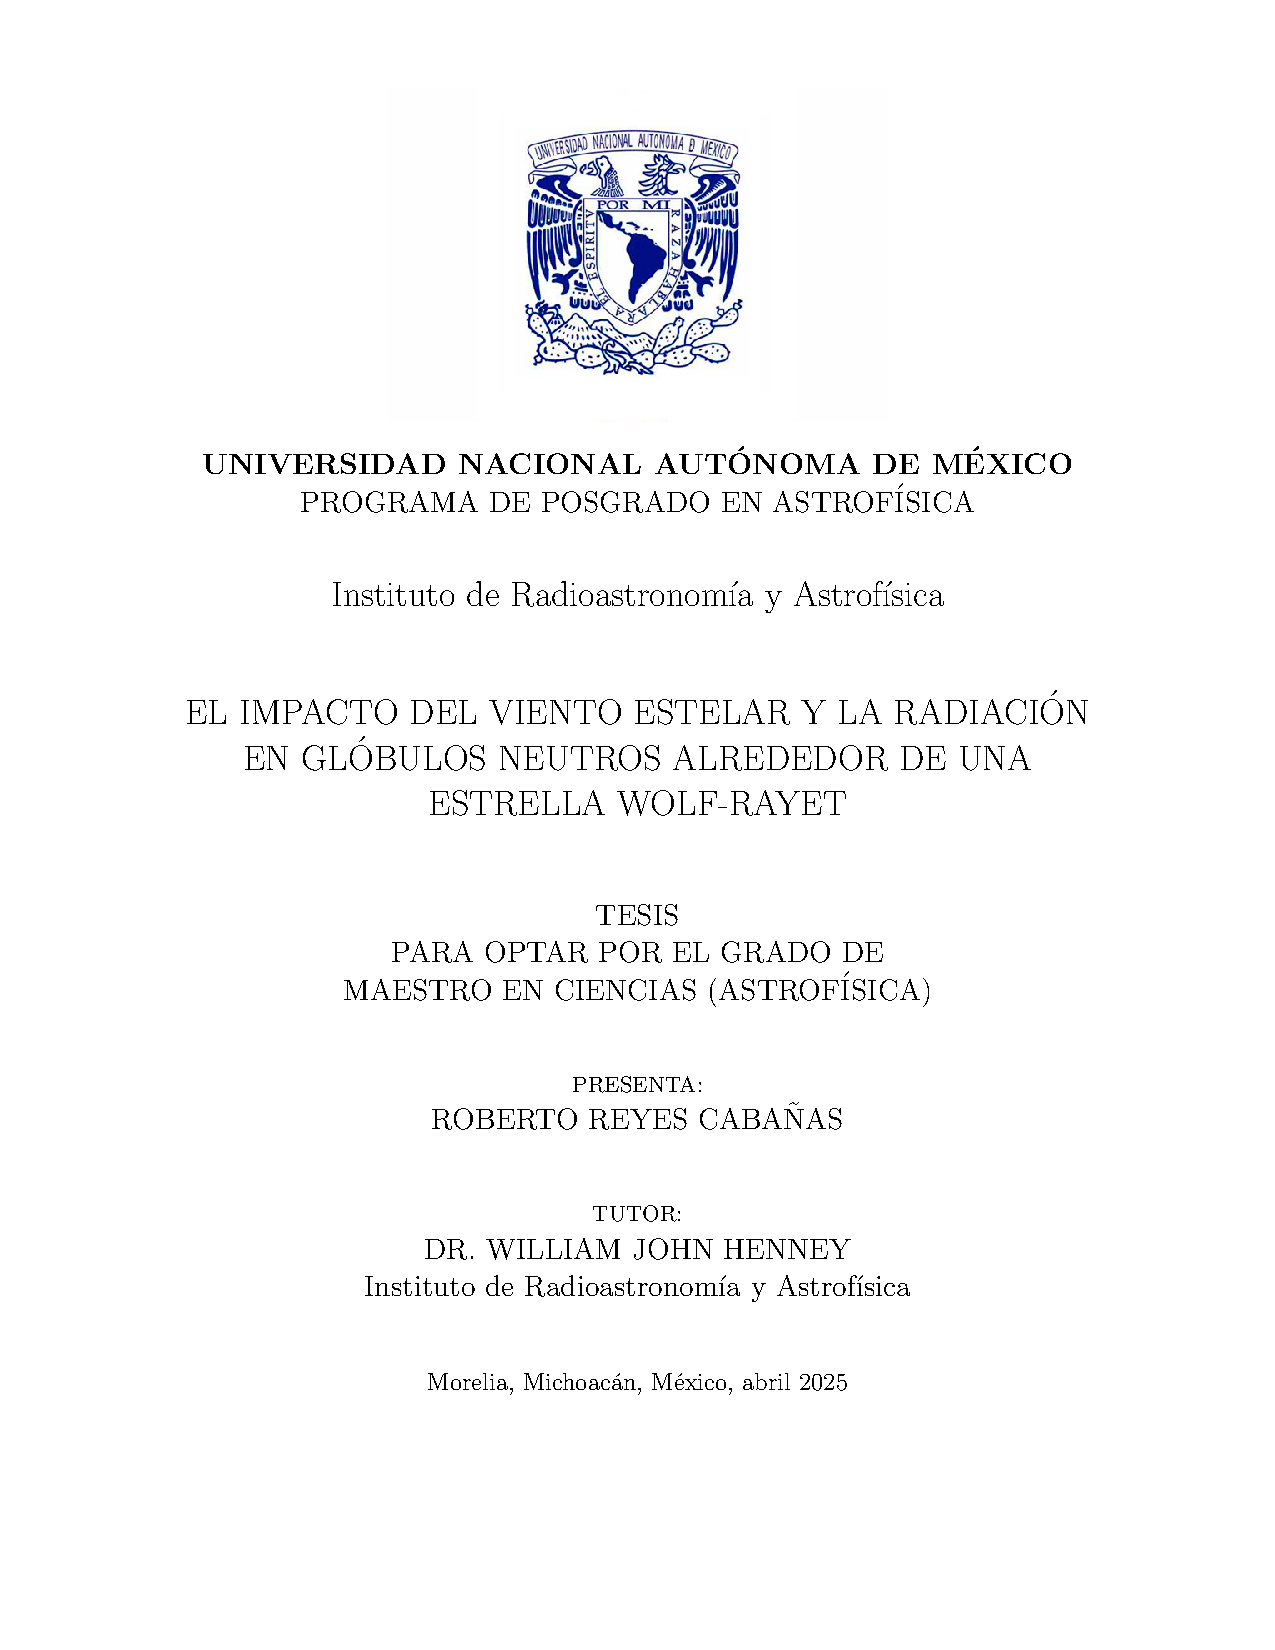
\includepdf[scale=1,pagecommand={}]{Portada_final.pdf}
\end{titlepage}


\chapter*{Abstract}

The circumstellar nebula M1-67 around the Wolf–Rayet star WR~124
contains hundreds of small neutral globules, as revealed by recent
images from the \textit{James Webb Space Telescope} (JWST). The
ionized emission of the nebula displays an intricate pattern of shells
and filaments, many of which appear associated with the globules but
displaced toward the central star. We propose a simple model for the
nebula in which photoevaporative flows from the irradiated surfaces of
the globules interact with the stellar wind of the Wolf–Rayet star to
form hemispherical emission shells. We test this model against JWST
and H$\alpha$ images of the nebula obtained with the \textit{Hubble Space
  Telescope} (HST), finding good agreement for the best-observed and
most isolated globules. The model provides a physical explanation for
the observed morphology of the nebula and globules, and suggests that
the globules are hydrodynamically shielded from the stellar wind by
the photoevaporative flows. We derive an independent estimate of the
stellar wind strength, which is consistent with values previously
obtained from stellar atmosphere modeling. We are also able to
constrain the three-dimensional distribution of the globules.

% \chapter*{Agradecimientos}

% A la persona que más me gustaría darle las gracias es a mi asesor,
% el Dr. Will. Él me supo guiar durante toda la maestría y estuvo ahí
% para mí siempre, sobre todo en los momentos más difíciles. Gracias a
% él, mi aventura en el mundo de la astronomía ha sido la más
% maravillosa que he tenido. Gracias doctor por toda su paciencia,
% apoyo y conocimiento que me compartió.

% También quisiera agradecer a la UNAM en general. Por aceptarme en el
% posgrado, lo cual para mí fue todo un reto. Por darme todas las
% comodidades para llevar a cabo mis estudios y compartirlo con la
% gente. Al campus Morelia porque ahí conocí a mi maestra de baile
% Lupita y a todos mis amiguitos, a quienes aprecio con toda mi alma.
% Con ustedes aprendí que no es necesario voltear al cielo para ver
% las estrellas, y menos si es para verlas bailar. Al IRyA por darme
% todo su apoyo incondicional, y sobre todo a los de divulgación, que
% aunque no lo crean, en sus eventos yo siempre me emocionaba tanto
% como los niños. A mamá Karin por toda su paciencia y cariño. También
% a mis compañeros de clase quienes siempre estuvieron ahí,
% literalmente.

% Quiero agradecer a mis sinodales por su tiempo, sugerencias y
% comentarios. Con su ayuda mejoré mucho mi trabajo. Gracias Toala! ya
% que por tu culpa me divertí mucho con este proyecto que tanto me
% fascinó.

% Agradezco a CONAHCYT por el apoyo financiero brindado para mis
% estudios e investigaciones. También al proyecto PAPIIT IN109823 de
% DGAPA por el apoyo financiero para hacer posible este trabajo.

% Finalmente, Gracias Dra. Gloria por coincidir en esta vida y
% mostrarme lo maravilloso que es este universo.

\chapter*{Acknowledgements}

The person I most wish to thank is my advisor, Dr.~Will. He guided me
throughout the entire master’s program and was always there for me,
especially in the most difficult moments. Thanks to him, my adventure
in the world of astronomy has been the most wonderful I have ever
experienced. Thank you, Doctor, for all the patience, support, and
knowledge you shared with me.

I would also like to thank UNAM in general: for accepting me into the
graduate program, which for me was quite a challenge; for providing
all the facilities I needed to carry out my studies; and for giving me
the chance to share them with others. To the Morelia campus, because
there I met my dance teacher Lupita and all my dear friends, whom I
cherish with all my heart. With you I learned that it is not necessary
to look up at the sky to see the stars—especially if it is to watch
them dance. To IRyA for giving me its unconditional support, and
especially to the outreach team, because although you may not believe
it, at your events I was always as excited as the children. To mamá
Karin for all her patience and affection. Also to my classmates, who
were always there—literally.

I want to thank my committee members for their time, suggestions, and
comments. With your help I greatly improved my work. Thanks,
Toalá!—since it was your fault that I had so much fun with this
project that fascinated me so much.

I am grateful to CONAHCYT for the financial support provided for my
studies and research. Also to the PAPIIT project IN109823 of DGAPA for
the financial support that made this work possible.

Finally, thank you, Dra.~Gloria, for crossing paths with me in this
life and showing me how wonderful this universe is.

\newpage

\tableofcontents

\newpage

\chapter{Introduction}\label{Capitulo 1:introduccion}

\textit{Globules} are dense concentrations of gas and dust in the
interstellar medium that are thought to form through thermal
instabilities, gravitational collapse, or turbulence
\citep{Ballesteros:2011,Padoan:2002}. These globules can arise in
regions of massive star formation or in nebulae around evolved stars,
such as planetary nebulae \citep{O'Dell:2007}.

In general, globules show a wide range of sizes. For example, when we
refer to globules in regions of massive star formation, they are
commonly large, $\sim$\SI{0.1}{pc} \citep{Schenider:2016}, whereas in
nebulae around evolved stars they are smaller, $\sim$\SI{e-2}{pc}
\citep{GFGahm:2013}.

The first globules were observed by Bart Bok in 1940. As we can see in
Figure \ref{fig:Banard}, because the background stars are reddened by
dust, these globules appear as dark clouds, given their large amounts
of neutral gas and dust. The globules contain primarily molecular
hydrogen in their interiors, and may also harbor other molecules
\citep{Amin:2005, DFrancesco:2002}. Although star formation can occur
inside them, the ionizing radiation from such stars cannot be observed
because it is absorbed by the neutral hydrogen (both molecular and
atomic) and the dust between the stars and the observer. For this
reason, they appear dark.

When globules are found in regions of massive star formation, they can
interact with the ultraviolet (UV) radiation from nearby young massive
stars, or with the radiation of the central star if the globules are
in a circumstellar nebula. In such cases the ionization front can be
seen as a bright rim of emission (see Figures \ref{fig:Pillars} and
\ref{fig:nudos}).

\begin{figure}[htb]
    \centering
    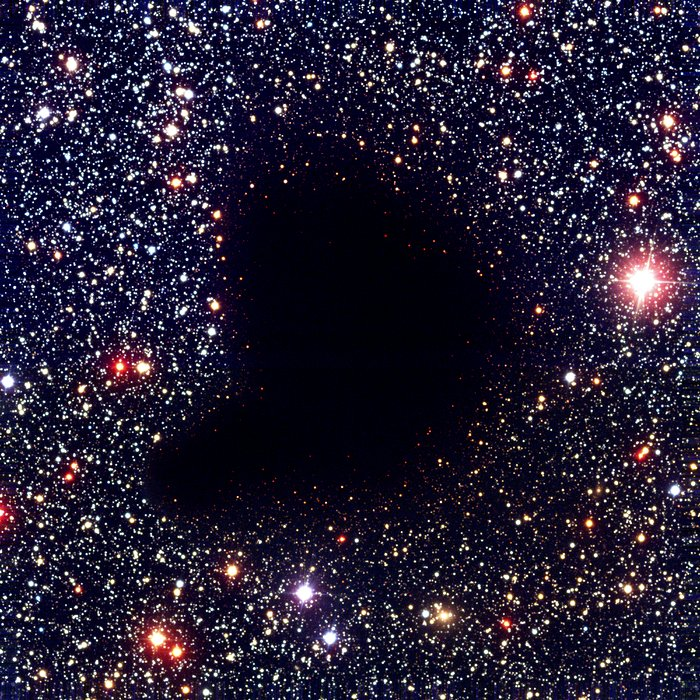
\includegraphics[width=0.85\textwidth]{images Chapter 1/C1_Bok_globule.jpg}
    \caption{Example of a Bok globule. Image of Barnard 68 taken with
      the Very Large Telescope FORS1 at 440 nm, 557 nm, and 768 nm,
      with an angular size of \ang{;6.83;}$\times$\ang{;6.83;}. A dark
      region can be seen, which is the globule itself, together with
      the apparent reddening of stars caused by dust on the globule’s
      surface. In this image there is no evidence of external
      photoevaporation from nearby stars \citep{Alves:2001}.}
    \label{fig:Banard}
\end{figure}

This interaction between stars and globules can occur on different
scales, giving rise to a wide variety of structures. Among the largest
are those that resemble columns, pillars, or “elephant trunks,” as
they are known in the literature. These can reach sizes of
$\sim$\SI{1}{pc} and densities of order \SI{e3}{cm^{-3}}. Such
interactions can also occur within H\,{\sc ii} regions, as shown in
Figure \ref{fig:Pillars}.

\begin{figure}[htb]
    \centering
    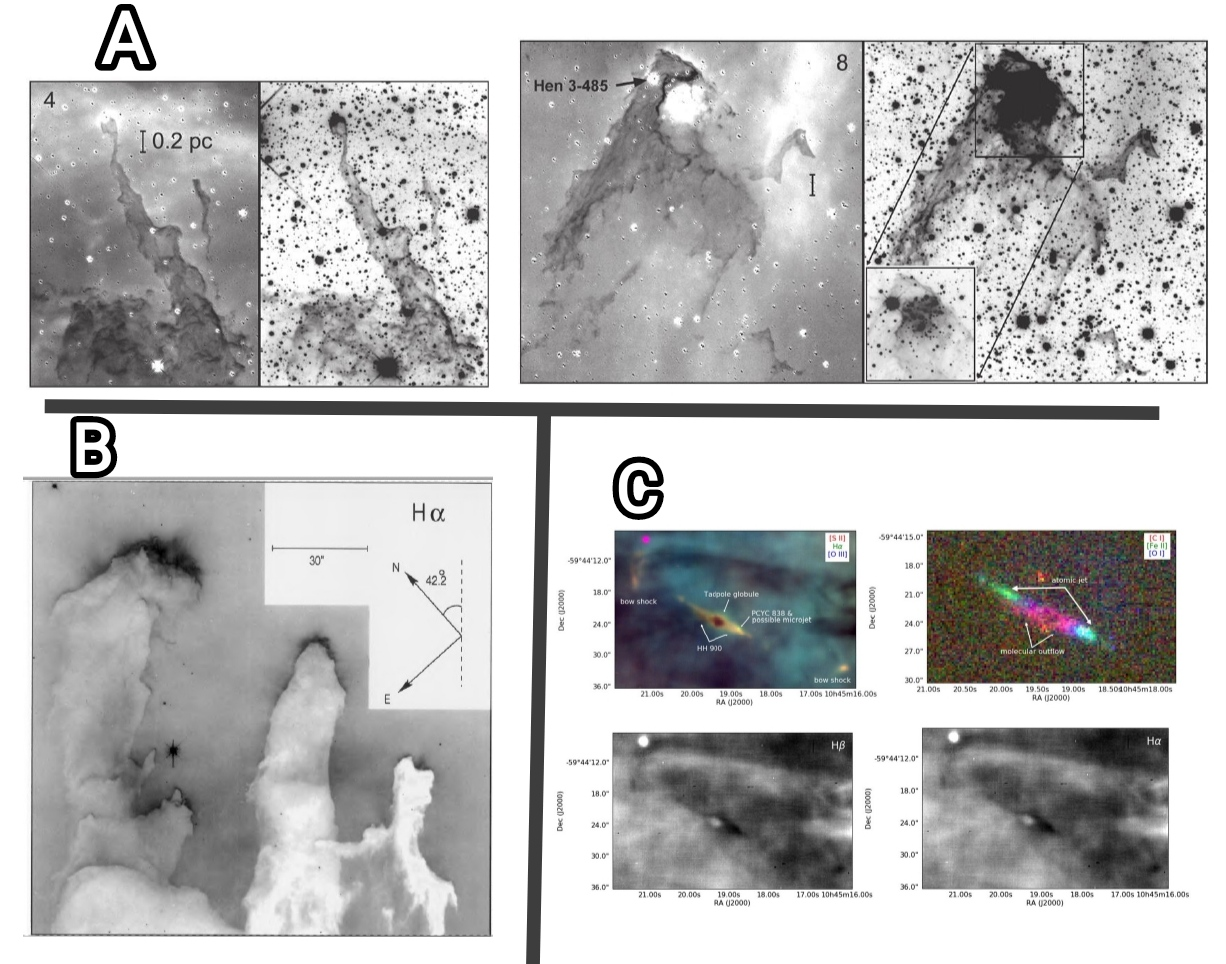
\includegraphics[width=1 \textwidth]{images Chapter 1/C1_Pillars.jpg}
    \caption{\textbf{A:} Two examples of pillars. In each case, the
      right-hand image is observed at \SI{2.12}{\mu m} (\SI{}{H_2})
      and the left-hand image shows \SI{}{H_2-Br_{\gamma}}
      \citep{Hartigan:2015}. \textbf{B:} An example of an elephant
      trunk. This is an image of M16 taken with WFPC2 using the F656N
      filter; the \SI{30}{\arcsecond} bar corresponds to
      \SI{9e17}{cm} (\SI{0.29}{pc}) \citep{JJHester:1996}. \textbf{C:}
      The outflow of the Tadpole globule, consisting of the HH900
      jet+outflow system. The lower panel shows the object in
      \SI{}{H\alpha} with the continuum \citep{MeganReiter:2019}.}
    \label{fig:Pillars}
\end{figure}

On smaller scales are the so-called EGGs (Evaporating Gaseous
Globules), which have sizes of $\sim$\SI{e-2}{pc}, and the proplyds,
which are $\le\SI{e-2}{pc}$. These globules are found not only in star
forming regions, but also in nebulae around evolved stars, where they
are more commonly known as \textit{knots}. An example of this is panel
\textbf{D} in Figure \ref{fig:nudos}. In this work we will study in
greater detail the knots present in a nebula surrounding a particular
evolved star.

\begin{figure}[htb]
    \centering
    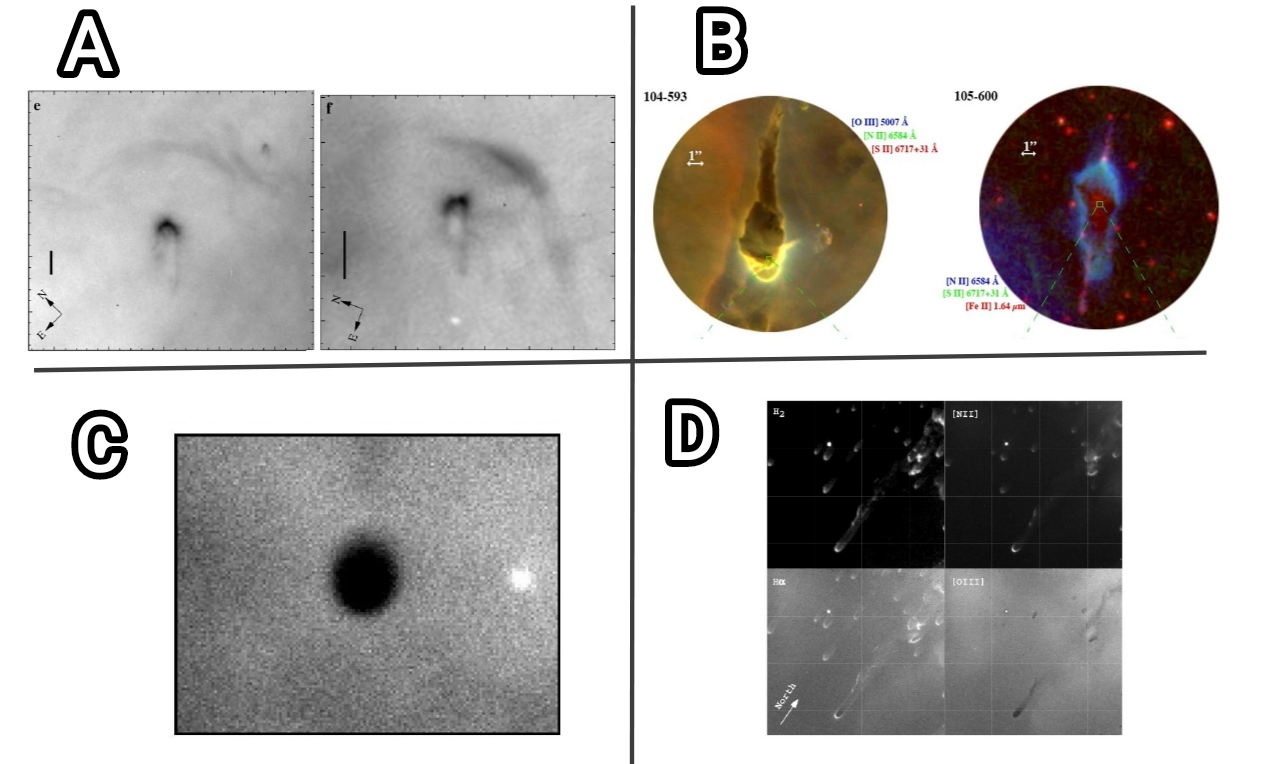
\includegraphics[width=1 \textwidth]{images Chapter 1/C1_Globulettes.jpg}
    \caption{\textbf{A:} Proplyds with their bow shocks in Orion,
      observed with the HST Planetary Camera. The black bar indicates
      a length of \SI{1}{\arcsecond}, corresponding to 430 AU
      (\SI{2e-3}{pc}) \citep{Garcia-Arredondo:2001}. \textbf{B:}
      Examples of EGGs in Carina, observed with WFC3, ACS, and WFPC2.
      The white bars of \SI{1}{\arcsecond} correspond to a physical
      size of \SI{e-2}{pc} \citep{Mesa-Delgado:2016}. \textbf{C:} The
      dense globulette RN88 seen in \SI{}{H\alpha} with a diameter of
      \SI{6}{\arcsecond} (\SI{4e-2}{pc}) in the Rosette Nebula
      \citep{GFGahm:2013}. \textbf{D:} Examples of knots in the Helix
      Nebula. The mosaics cover \SI{47.5}{\arcsecond}$\times$
      \SI{44.8}{\arcsecond} (\SI{4.76e-2}{pc}$\times$\SI{4.49e-2}{pc})
      \citep{O'Dell:2007}.}
    \label{fig:nudos}
\end{figure}

% \section{Flujos de fotoevaporación ionizada} \label{Sec:fluijos fotoevaporativos}

% Todos los ejemplos de las Figuras \ref{fig:Banard}, \ref{fig:Pillars}
% y \ref{fig:nudos} se encuentran ya sea en regiones de formación
% estelar o en nebulosas alrededor de estrellas evolucionadas. Lo
% interesante en todos estos ejemplos es la forma que toman al
% interaccionar con las estrellas más masivas que se encuentran cerca,
% esto para los glóbulos que se encuentran en regiones de formación
% estelar. Mientras que los que se encuentran en nebulosas planetarias
% interactúan con la estrella evolucionada. Durante estas interacciones,
% en algunos casos podemos ver lo que se conoce como \textit{flujos
%   fotoevaporativos}, los cuales explicaremos mejor a continuación.

% Cuando la radiación ionizante incide en la superficie del glóbulo,
% este comienza a ionizar el gas neutro. A este flujo de gas ionizado
% que sale de la base del glóbulo y que viaja en dirección a la fuente
% ionizante se le conoce como flujo fotoevaporativo.

% En el caso de las regiones de formación estelar podemos considerar una
% estrella masiva y una nube densa de gas neutro. Por lo que para poder
% ver el flujo fotoevaporativo es necesario que la estrella sea masiva,
% o que tenga un gran flujo ionizante como para poder ionizar el gas
% neutro, de lo contrario no podremos ver el flujo fotoevaporativo.
% Recordemos que en las regiones de formación estelar hay muchas
% estrellas nuevas de baja masa que emiten principalmente en radio o
% infrarrojo, por lo que no todas las estrellas nuevas pueden ionizar el
% gas neutro.

% \cite{OortySpitzer_1955} explican de manera detallada como es la
% interacción entre una estrella tipo O y una nube interestelar de gas
% neutro. La cual se puede observar en regiones de formación estelar
% masiva. Ellos consideran tres elementos importantes para esto: La
% estrella ionizante, la nube interestelar de gas neutro y la región que
% hay entre la estrella y la nube interestelar. La nube interestelar
% debe ser mucho más densa y fría que la región que hay entre la
% estrella y la nube como vemos en la Figura \ref{kahn_zones}.

% \begin{figure}[htb]
%     \centering
%     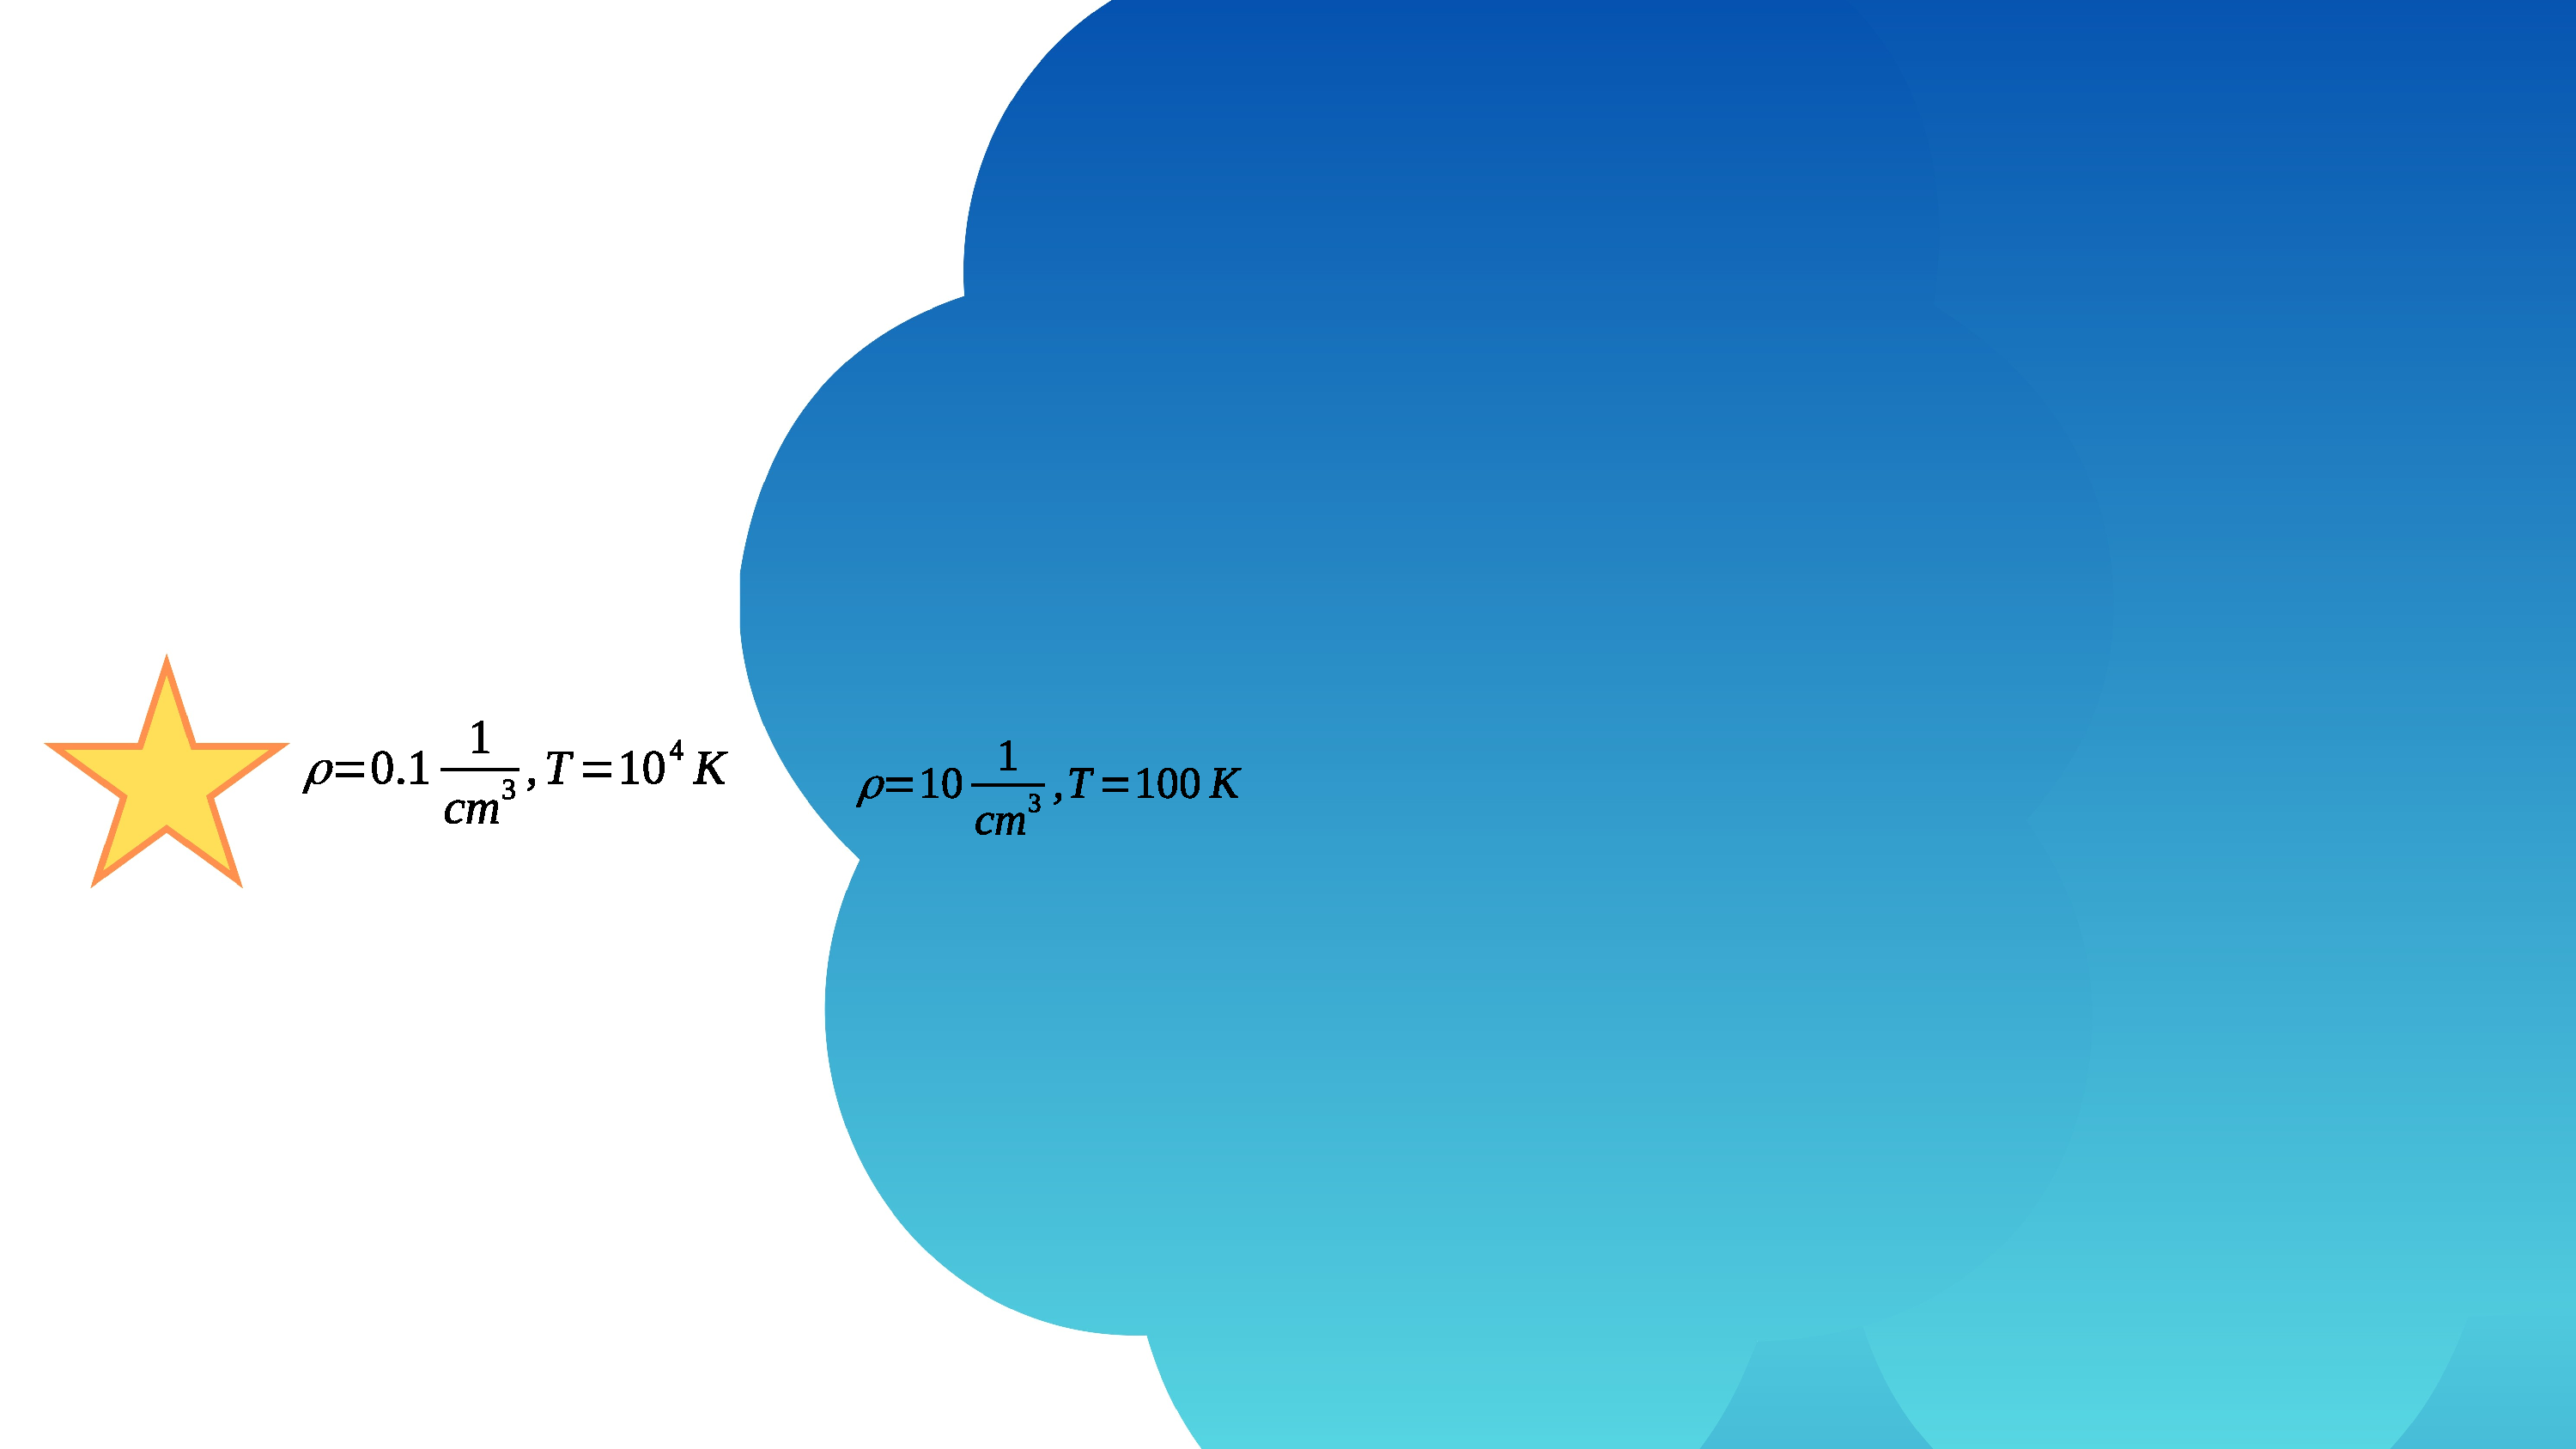
\includegraphics[width= \textwidth]{artesanales/ImgFi01-5.pdf}
%     \caption{Esquema inicial utilizado en \cite{OortySpitzer_1955},
%       donde podemos apreciar que la nube es más fría y densa que la
%       región que hay entre la nube y la estrella.}
%     \label{kahn_zones}
% \end{figure}

% Cuando la radiación UV comienza a calentar el gas de la nube, el gas
% ionizado comienza a expandirse en dirección a la estrella, esto ya que
% en esta dirección la densidad es menor que la de la nube y puede
% expandirse libremente (Figura \ref{fig:evolucion de la nube}).

% \begin{figure}[htb]
%     \centering
%     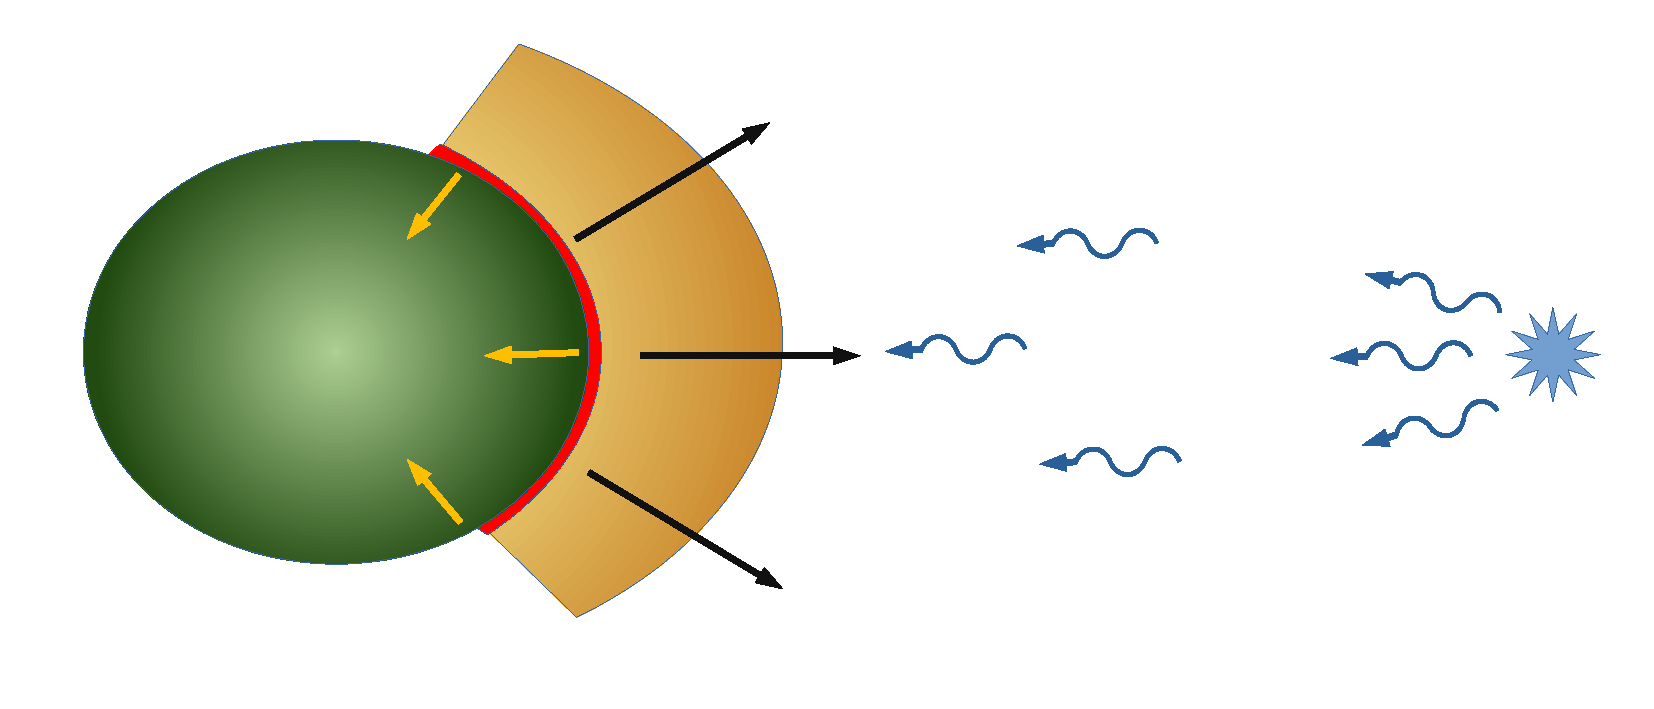
\includegraphics[width= \textwidth]{ultimos/implosion_inicial.pdf}
%     \caption{Esquema de la implosión inicial. Cuando la radiación
%       ionizante (flechas azules) inciden en el glóbulo (color verde)
%       produce que el gas ionizado (color naranja) viaje en dirección a
%       la estrella como lo muestran las flechas negras. En esta fase se
%       produce un choque interno que hará que la nube se comprima.
%       Tanto el choque como el frente de ionización (color rojo) viajan
%       hacia el centro del glóbulo como lo muestran las flechas
%       amarillas.}
%     \label{fig:evolucion de la nube}
% \end{figure}

% En un inicio esta radiación ioniza el gas neutro de la nube a una tasa
% muy rápida. Esto causa que una gran cantidad partículas ionizadas,
% provenientes de la nube, viajen en dirección a la estrella. Conforme
% esto va evolucionando se va formando una capa aislante alrededor de la
% nube \citep{OortySpitzer_1955}. Esta capa aislante esta conformada por
% el gas ionizado, y puede proteger a la nube de flujos o vientos
% externos, así como de la radiación.

% Durante esta interacción tenemos tanto un frente de ionización como un
% choque interno que viajan a través de la nube a la parte trasera (ver
% Figura \ref{fig:evolucion de la nube}). Al inicio estos dos tienen una
% velocidad similar de $\sim\SI{10}{km.s^{-1}}$, pero una vez que las
% recombinaciones se vuelven importantes en la capa aislante, el frente
% de ionización comienza a desacelerar. Mientras que el choque interno
% hace que la nube se comprima \citep{Bertoldi_1989}.

% No siempre podemos ver un flujo fotoevaporativo por parte de las nubes
% en este tipo de interacción, para esto \cite{Bertoldi_1989} nos dice
% que si el parámetro de ionización, definido como
% \begin{equation}
%     \Gamma  \equiv \frac{F_\mathrm{i}}{n_0 c}
% \end{equation}
% donde $F_\mathrm{i}$ es el flujo incidente del continuo de Lyman,
% $n_0$ la densidad del gas neutro, y $c$ la velocidad de la luz, es
% menor que \SI{e-7}{}, entonces la radiación ionizante incidente no
% tendrá un efecto dinámico sobre la nube por lo que no tendremos un
% flujo fotoevaporativo por parte de la nube. Por otro lado, si
% \begin{equation}
%     \delta'\equiv\frac{F_\mathrm{i}}{2\alpha_\mathrm{i} r_0 n_0^2}>1
% \end{equation}
% donde $\alpha_\mathrm{i}$ es el coeficiente de recombinación a todos los
% estados, excepto al nivel base y $r_0$ el radio de la nube, entonces
% la nube se ionizará por completo, esto ya que el flujo ionizante es
% mayor que las recombinaciones.

\section{Ionized photoevaporative flows} 
\label{Sec:fluijos fotoevaporativos}

All the examples in Figures \ref{fig:Banard}, \ref{fig:Pillars}, and
\ref{fig:nudos} occur either in regions of star formation or in
nebulae around evolved stars. What is interesting in all these cases
is the way they interact with the most massive stars in their
vicinity, for globules found in star-forming regions, or with the
evolved central star in planetary nebulae. During these interactions,
in some cases we can see what are known as \textit{photoevaporative
  flows}, which we explain in more detail below.

When ionizing radiation strikes the surface of a globule, it begins to
ionize the neutral gas. The resulting flow of ionized gas that streams
away from the base of the globule and travels toward the ionizing
source is known as a photoevaporative flow.

In the case of star-forming regions, we can consider a massive star
and a dense cloud of neutral gas. In order to observe a
photoevaporative flow, the star must be massive, or must have a large
ionizing flux capable of ionizing the neutral gas. Otherwise, the
photoevaporative flow will not be visible. Recall that in star-forming
regions there are many new low-mass stars that emit mainly in radio or
infrared, so not all young stars are capable of ionizing the neutral
gas.

\cite{OortySpitzer_1955} give a detailed explanation of the
interaction between an O-type star and a cloud of neutral interstellar
gas, as observed in regions of massive star formation. They consider
three key elements: the ionizing star, the neutral interstellar cloud,
and the region between the star and the cloud. The interstellar cloud
must be much denser and colder than the intervening region, as shown
in Figure \ref{kahn_zones}.

\begin{figure}[htb]
    \centering
    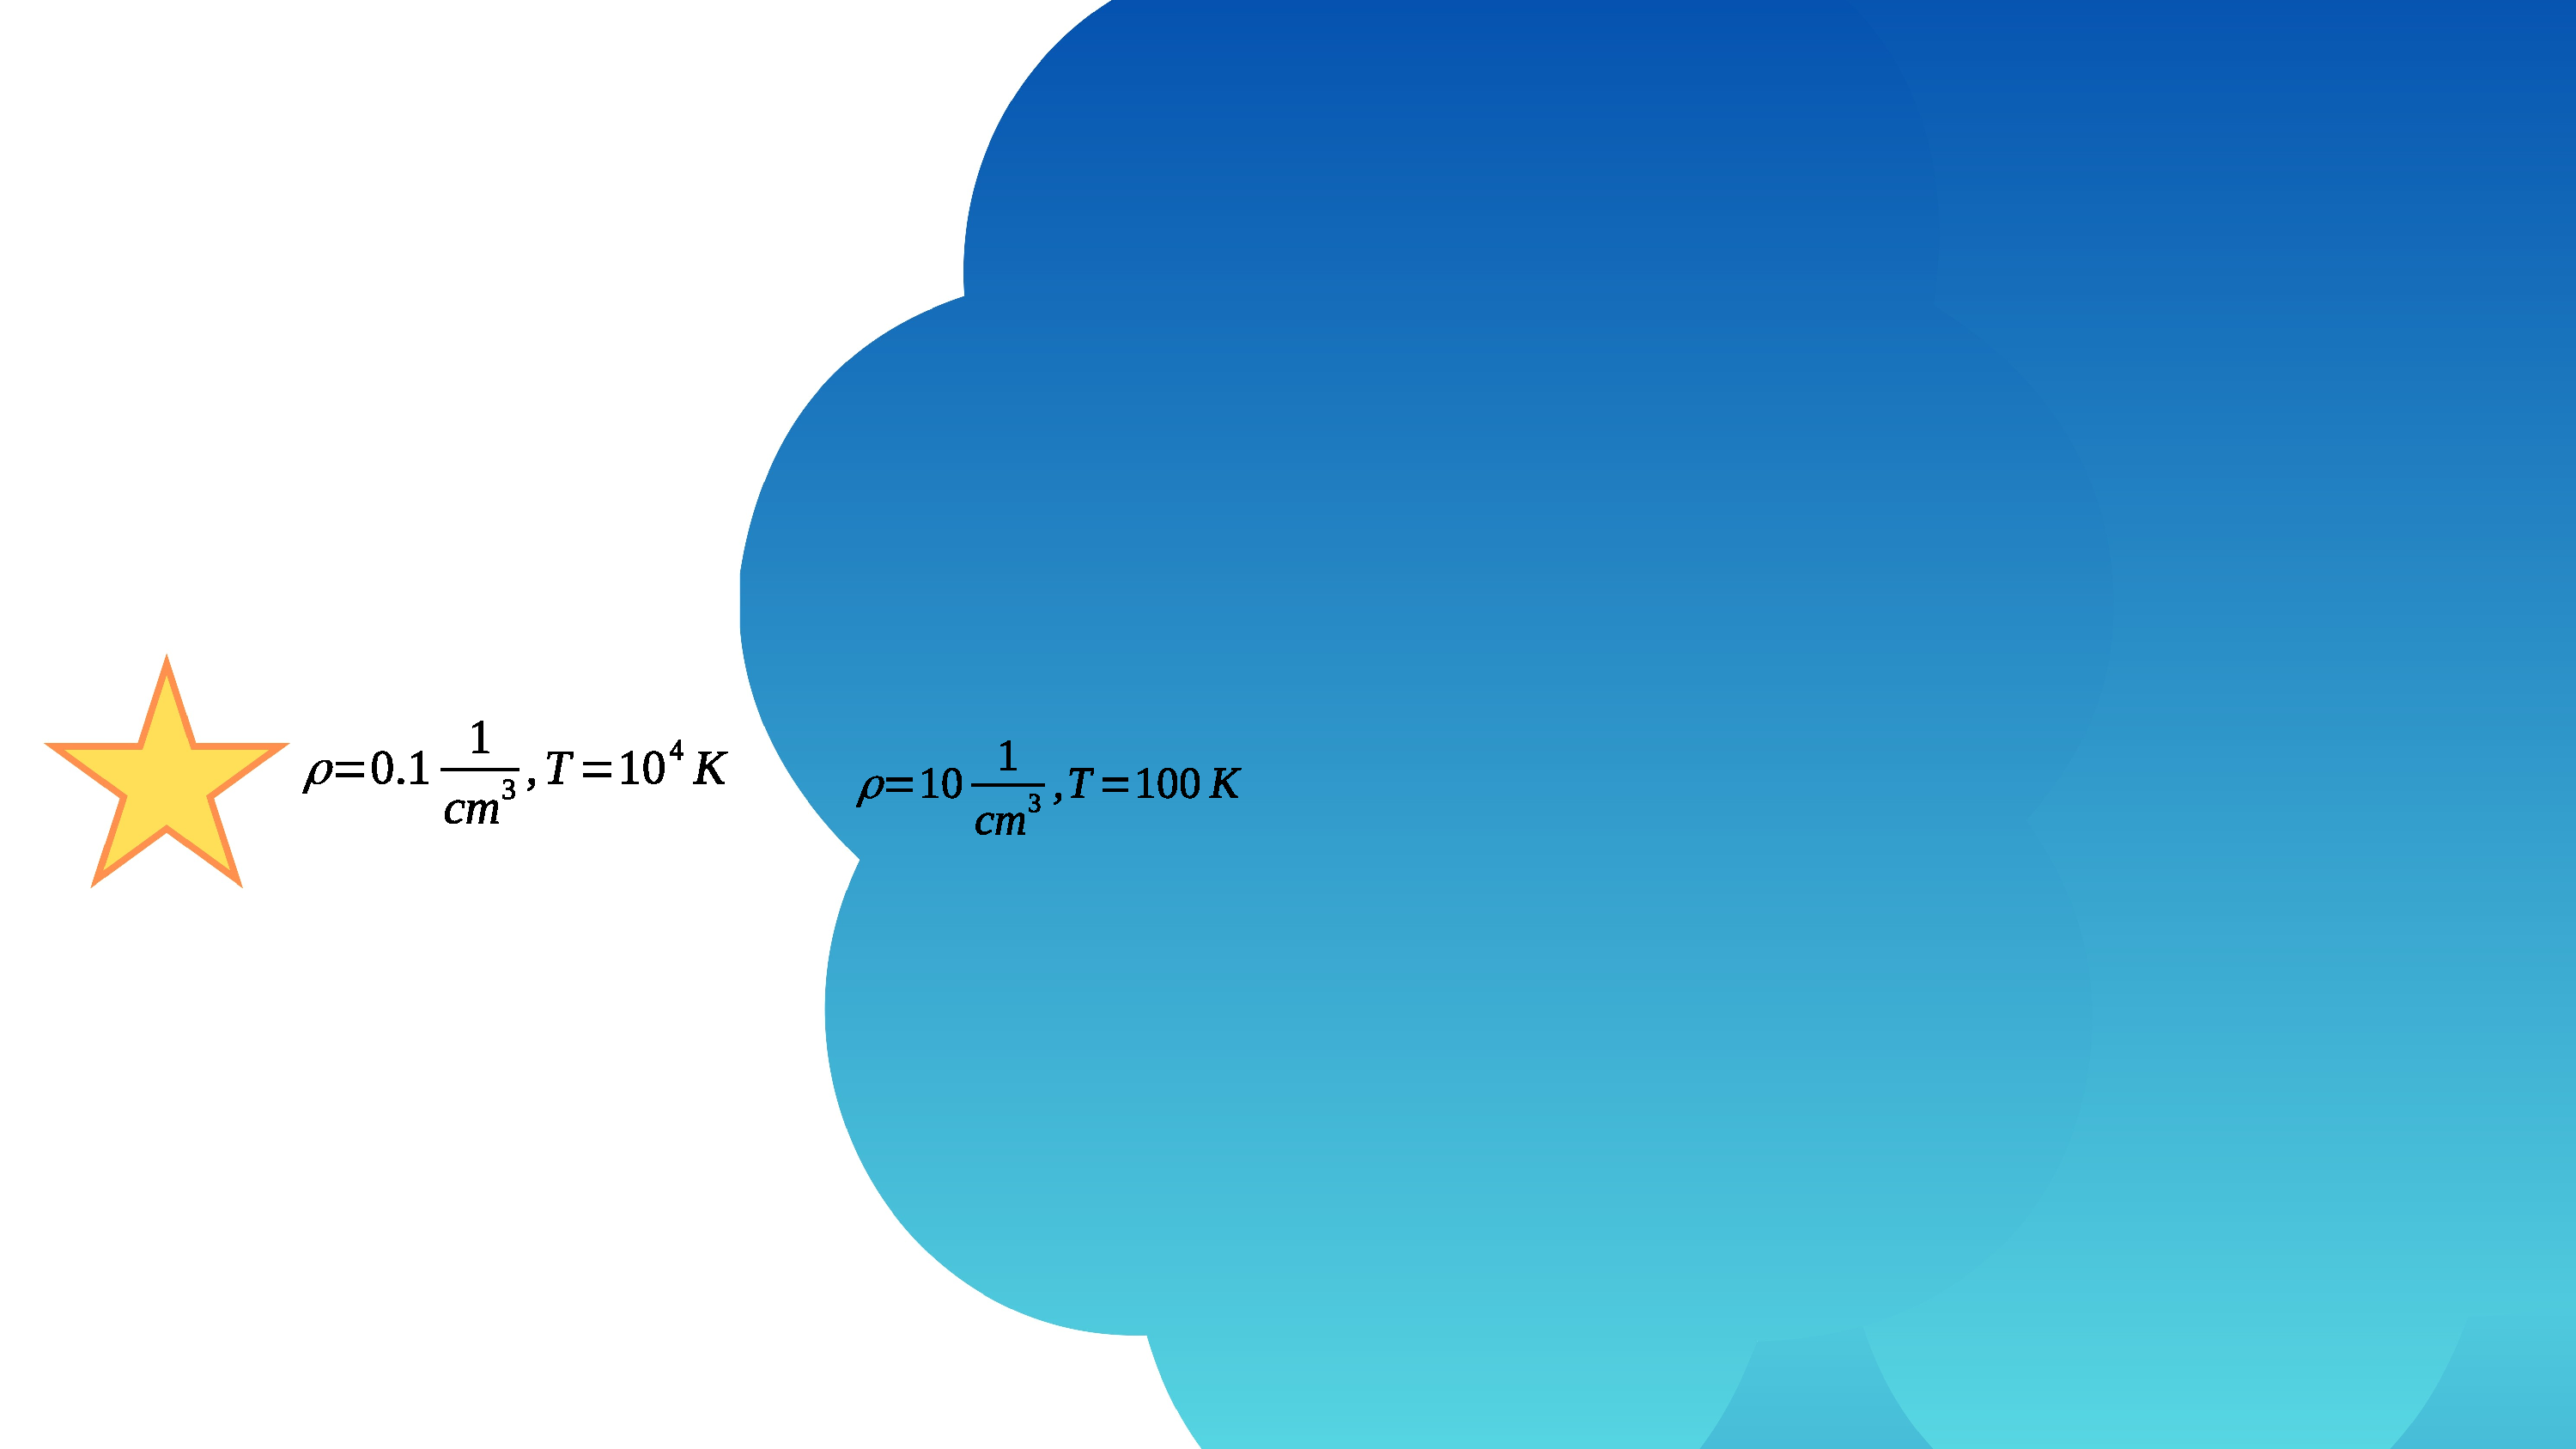
\includegraphics[width= \textwidth]{artesanales/ImgFi01-5.pdf}
    \caption{Initial schematic used in \cite{OortySpitzer_1955}, in
      which the cloud is colder and denser than the region between the
      cloud and the star.}
    \label{kahn_zones}
\end{figure}

When UV radiation begins to heat the gas in the cloud, the ionized gas
expands toward the star, since in that direction the density is lower
than in the cloud and the gas can expand freely (see Figure
\ref{fig:evolucion de la nube}).

\begin{figure}[htb]
    \centering
    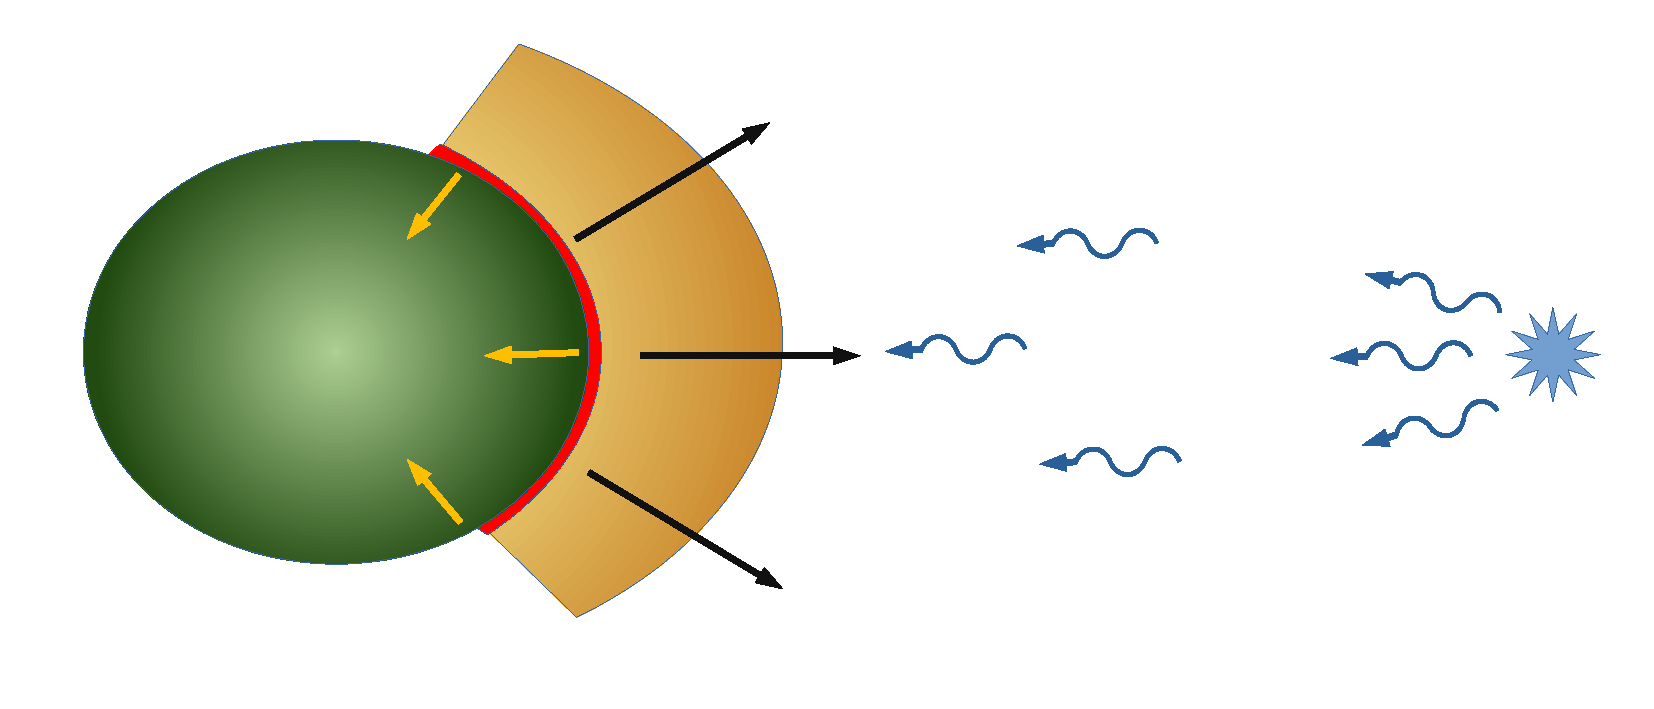
\includegraphics[width= \textwidth]{ultimos/implosion_inicial.pdf}
    \caption{Schematic of the initial implosion. When ionizing
      radiation (blue arrows) strikes the globule (green), it causes
      ionized gas (orange) to flow toward the star, as shown by the
      black arrows. In this phase an internal shock is produced that
      compresses the cloud. Both the shock and the ionization front
      (red) travel toward the center of the globule, as indicated by
      the yellow arrows.}
    \label{fig:evolucion de la nube}
\end{figure}

At first this radiation ionizes the neutral gas of the cloud at a very
rapid rate. As a result, a large number of ionized particles, coming
from the cloud, flow toward the star. As the process evolves, an
insulating layer forms around the cloud \citep{OortySpitzer_1955}.
This insulating layer is composed of ionized gas and can protect the
cloud from external flows or winds, as well as from radiation.

During this interaction there are both an ionization front and an
internal shock that travel through the cloud toward the rear (see
Figure \ref{fig:evolucion de la nube}). Initially, these two have a
similar velocity of $\sim\SI{10}{km.s^{-1}}$, but once recombinations
in the insulating layer become important, the ionization front begins
to decelerate. Meanwhile, the internal shock compresses the cloud
\citep{Bertoldi_1989}.

It is not always possible to observe a photoevaporative flow from
clouds in this type of interaction. For this,
\cite{Bertoldi_1989} note that if the ionization parameter, defined as
\begin{equation}
    \Gamma  \equiv \frac{F_\mathrm{i}}{n_0 c}
\end{equation}
where $F_\mathrm{i}$ is the incident flux of Lyman continuum photons,
$n_0$ is the density of neutral gas, and $c$ is the speed of light, is
less than \SI{e-7}{}, then the incident ionizing radiation will have
no dynamical effect on the cloud, and no photoevaporative flow will be
produced. On the other hand, if
\begin{equation}
    \delta'\equiv\frac{F_\mathrm{i}}{2\alpha_\mathrm{i} r_0 n_0^2}>1
\end{equation}
where $\alpha_\mathrm{i}$ is the recombination coefficient to all
states except the ground state, and $r_0$ is the radius of the cloud,
then the cloud will be completely ionized, since the ionizing flux is
greater than the recombinations.


\section{Wolf--Rayet stars and their winds}

Wolf--Rayet (WR) stars are the evolved descendants of massive stars,
such as O-type stars. These WR stars typically have masses of
10--\SI{25}{\msun} and are characterized by intense emission lines and
free--free emission at IR--mm--cm wavelengths \citep{crowther:2007}.
They also have high mass-loss rates, $\sim$2--\SI{10e-5}{\msun/yr},
driven by their strong stellar winds, which can reach velocities of
$\sim$\SI{1000}{km/s}, producing their broad emission lines
\citep{Hamman:2006}. They were named after Charles Wolf and Georges
Rayet, who first identified three stars in Cygnus with broad emission
lines of C, N, O, and He---the characteristic features of this class
\citep{WR:ref}.

These stars are classified according to the relative strengths of
their characteristic emission lines. \cite{VanDerHutch:2001} classify
them mainly as type WN when He and N are abundant, type WC when He and
C dominate, and type WO when He and O are abundant. Although many of
these stars show no hydrogen in their atmospheres, in some cases a
significant amount of H is detected, in which case the designation ``h''
is added \citep{SSM:1996}.

\section{The nebula M1-67}

M1-67 is the circumstellar nebula around the WR~124 star, which is of
type WN8h. Several studies have been carried out on the M1-67 nebula,
including three-dimensional models of its structure based on long-slit
spectroscopy \citep{Zavala:2022}. \cite{Marcel:2021} used the
$[\mathrm{S \scriptstyle{II}}]\lambda6717$ and $\lambda6731$ lines to
find that the electron density decreases with radius: close to the
star the electron density is $\sim$\SI{2000}{cm^{-3}}, while farther
away, at about \SI{40}{\arcsecond} (\SI{1.05}{pc}), it drops to
$\sim\SI{500}{cm^{-3}}$. \cite{Grosdidier:1998} found that the
H$\alpha$ surface brightness also decreases with radius as $r^{-0.8}$.
\cite{Mancherko:2010} measured an expansion velocity of
\SI{46}{km.s^{-1}} for the nebula using observations from 1997
\citep{Grosdidier:1998} and 2008, consistent with the measurement of
\cite{Zavala:2022}.

Figures \ref{fig:M1-67HST} and \ref{fig:M1-67JWST} show that this
nebula has a very complex structure. \cite{Grosdidier:1998} detected
some very bright and dense knots, but their nature was not clear. In
Chapter \ref{Chapter : 3} we will discuss in detail how these bright
and dense points are in fact globules located throughout much of the
nebula. These globules were revealed thanks to images from the James
Webb Space Telescope (JWST), which has higher resolution than the
Hubble Space Telescope (HST), and also offers a much greater variety
of filters.

Throughout this thesis we will use the data in Table
\ref{tab:parametros WR-124}. With the distance to the star, $D$, we
can derive physical distances as
\begin{equation}
    \left[\frac{R}{\mathrm{AU}}\right]=\left[\frac{D}{\mathrm{pc}}\right]\left[\frac{\theta}{\mathrm{arcsec}}\right]
\end{equation}
where $R$ is the desired physical distance and $\theta$ is the
separation measured directly from the observations in arcseconds. The
mass-loss rate, $\dot{M}$, and the terminal velocity of the stellar
wind, $v_\infty$, allow us to calculate the hydrodynamic (RAM)
pressure of the stellar wind, while the rate of ionizing photons from
the star is used to calculate the radiation pressure.

\begin{table}[htb]
    \centering
    \begin{tabular}{c c c}
        \toprule
        \multicolumn{3}{c}{Parameters of WR~124} \\ \midrule
         $D$ & 5.429$\pm$\SI{.54}{kpc} & J. Arthur, priv.~comm.\\
         $v_\infty$ & \SI{710}{km/s}  & \cite{Hamman:2006}\\
         $\dot{M}$ & $10^{-4.7}$\unit{M_\odot/yr}  & \cite{Crowther:1999}\\
         $S_*$ & \SI{1.25e49}{s^{-1}} & \cite{crowther:2007}  \\
         %$F_{H_\alpha}$ & \SI{3e-14}{erg.cm^{-2}.s^{-1}} & \cite{Grosdidier:1998}\\
         \bottomrule
    \end{tabular}
    \caption{Parameters of WR~124.}
    \label{tab:parametros WR-124}
\end{table}

\subsection{HST observations}

For the Hubble Space Telescope (HST) observations we used data from
the Hubble Legacy Archive. These are FITS images at calibration level
3, meaning they are mosaics created by combining multiple images to
cover a region of the sky\footnote{For more details see
  \url{https://hla.stsci.edu/hla_faq.html\#productlevels}}. We used
the F656N filter\footnote{Appendix \ref{App: Filtros} shows the range
  covered by this filter.} with the Wide Field and Planetary Camera 2
(WFPC2) to observe \unit{H\alpha} emission. We used the 1997 data from
proposal ID 6787, with a total exposure time of \SI{10 216}{s} from a
combination of 10 exposures. The 2008 data from proposal ID 11137 have
a total exposure time of \SI{4200}{s} from a combination of 8
exposures.

\begin{figure}[htb]
    \centering
    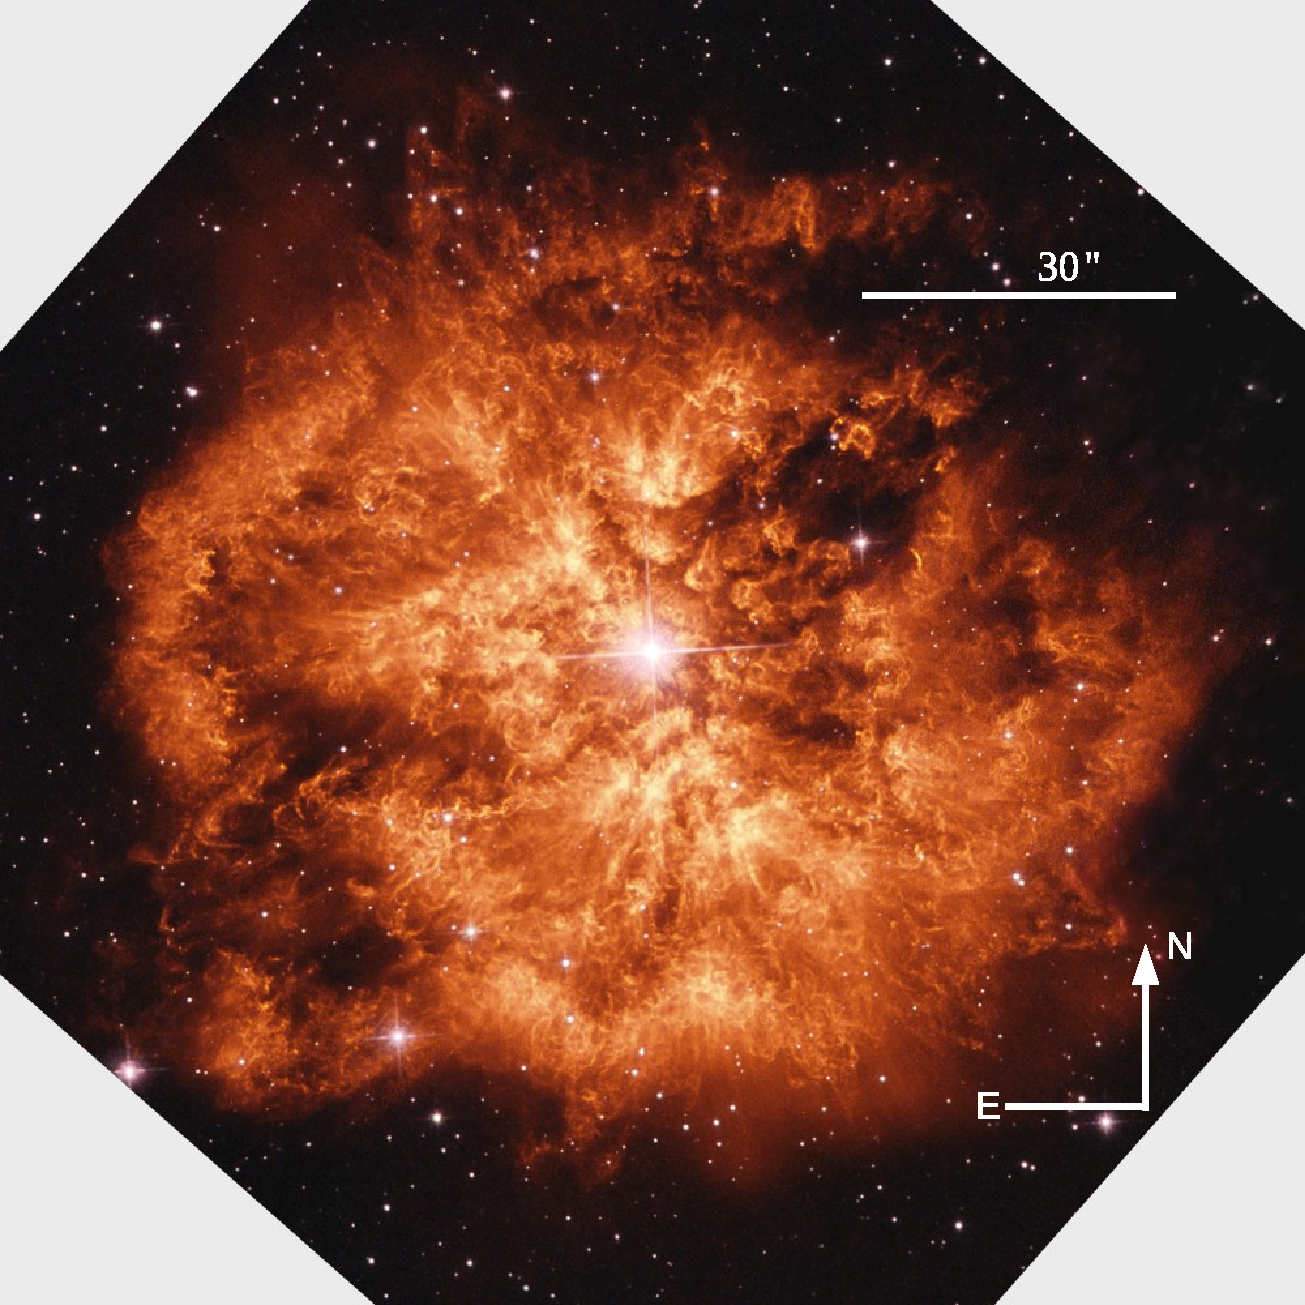
\includegraphics[width=0.9\textwidth]{ultimas correcciones/WR124_HST.pdf}
    \caption{Image of M1-67 in the \unit{H\alpha} filter
      \citep{Grosdidier:1998}. The \SI{30}{\arcsecond} scale
      corresponds to \SI{0.78}{pc}.
      https://esawebb.org/images/weic2307f/. The image has been
      rotated so that North is up and East is to the left.}
    \label{fig:M1-67HST}
\end{figure}

\subsection{JWST observations}

For the James Webb Space Telescope (JWST) observations we used data
obtained by Klaus M. Pontoppidan, proposal ID 2730. We used the NIRCam
filters F090W, F150W, F210M, F335M, F444W, and
F470N\footnote{Appendix \ref{App: Filtros} shows the wavelength range
  of each of these filters.}, with a total exposure time of
\SI{2662.72}{s}. These are level 3 images---mosaics combining multiple
exposures to cover a region of the sky---in FITS format.

The wide variety of JWST filters allows us to combine them to observe
different emission mechanisms, and its high resolution makes it
possible to resolve the detailed structures.

Unlike the H$\alpha$ image, the JWST observations use broad-band
filters. These bands include contributions from different emission
mechanisms: stellar continuum, some nebular emission lines, continuum
scattered by dust, thermal dust emission, and also emission from
polycyclic aromatic hydrocarbon (PAH) bands.

\begin{figure}[htb]
    \centering
    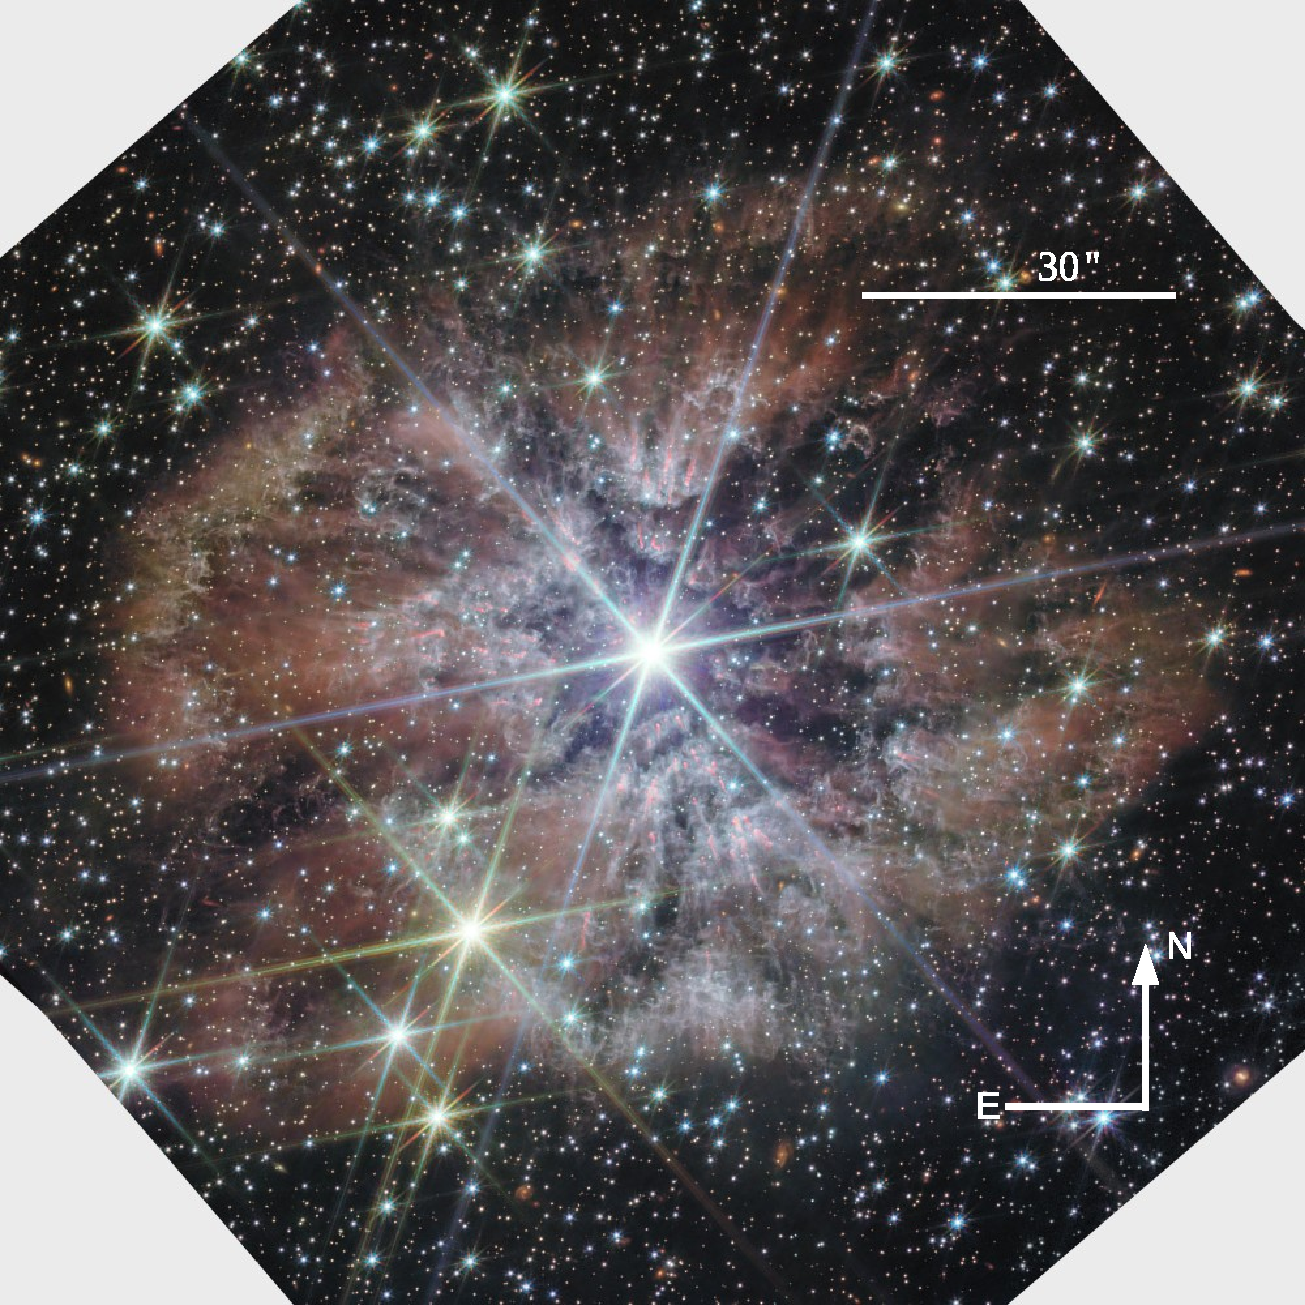
\includegraphics[width=0.9\textwidth]{ultimas correcciones/WR124_JWST.pdf}
    \caption{Image of M1-67 with JWST. Composite of filters f444w
      (gray), f335m (red), f210m (green), f150w (turquoise green), and
      f090w (blue). The \SI{30}{\arcsecond} scale corresponds to
      \SI{0.78}{pc}.
      https://www.flickr.com/photos/geckzilla/52757287572/. The image
      has been rotated so that North is up and East is to the left.}
    \label{fig:M1-67JWST}
\end{figure}

\section{Structure of the thesis}

In this thesis we propose a simple model to explain how the transonic
photoevaporative flow from a globule interacts with an external
pressure. We will apply this model to the knots in the M1-67 nebula,
and describe how the photoevaporative flow interacts with the
hydrodynamic (RAM) pressure of the stellar wind of WR~124.

In Chapter 2 we will see how the interaction between two supersonic
flows creates a thin shocked shell. Based on this, we describe a
steady-state hydrodynamic model in which the photoevaporative flow of
a globule interacts with an external pressure. In this interaction a
shocked shell can also be seen.

In Chapter 3 we will describe how we identified the knots in the M1-67
nebula, as well as observational evidence of the interaction between
the photoevaporative flow of the knots and the stellar wind of WR~124.

In Chapter 4 we will apply this model to the knots found in the
nebula. We will fit the radial brightness profiles in order to measure
the knots and their shocked shells. In addition, we can derive the
density of the ionized gas from the emission measure.

In Chapter 5 we will compare these results with the theoretical values
predicted by the proposed model. This comparison provides a clearer
understanding of the distribution of the knots in the nebula.

% \chapter{Modelos analíticos de flujos fotoevaporativos interactuando
%   con una presión externa}
% \chaptermark{Modelo analítico}\label{Chapter : Modelo}

% En este capítulo vamos a describir el modelo que se propone para
% explicar la interacción que hay entre el flujo fotoevaporativo de un
% glóbulo y una presión externa. Esta presión externa puede ser ejercida
% por la misma estrella que esta foto evaporando al glóbulo. Este modelo
% en principio se puede aplicar a cualquier tipo de glóbulo como los que
% se mencionaron en el Capítulo \ref{Capitulo 1:introduccion}.

% En este trabajo en especial vamos a tratar la interacción del flujo
% fotoevaporativo de los glóbulos\footnote{Llamaremos glóbulos a los
% nudos que hay en la nebulosa por simplicidad.} en la nebulosa M1-67 y
% la presión RAM por parte del viento estelar de la estrella WR 124. En
% el Capítulo \ref{Chapter : 3} hablaremos más acerca de cómo
% encontramos estos glóbulos en la nebulosa M1-67, por ahora nos
% enfocaremos solo en el modelo.

% Para esto hemos considerado que ya han pasado todas las fases
% mencionadas en la Sección \ref{Sec:fluijos fotoevaporativos} y ahora
% estamos en un equilibrio de ionización. La forma del glóbulo en este
% modelo será esférico por simplicidad.

% En esta interacción entre el flujo fotoevaporativo y el viento
% estelar, los cuales son supersónicos, se producen dos zonas chocadas y
% entre estas dos zonas una discontinuidad de contacto como se describe
% en la Figura \ref{fig:zones}. De estas zonas esperamos ver solo el
% flujo fotoevaporativo chocado y no el viento estelar chocado ya que
% este último es menos denso además de que es no radiativo y su longitud
% de enfriamiento (zona 3) es más grande que la región de interacción
% (zona 2).

% \begin{figure}[htb]
%     \centering    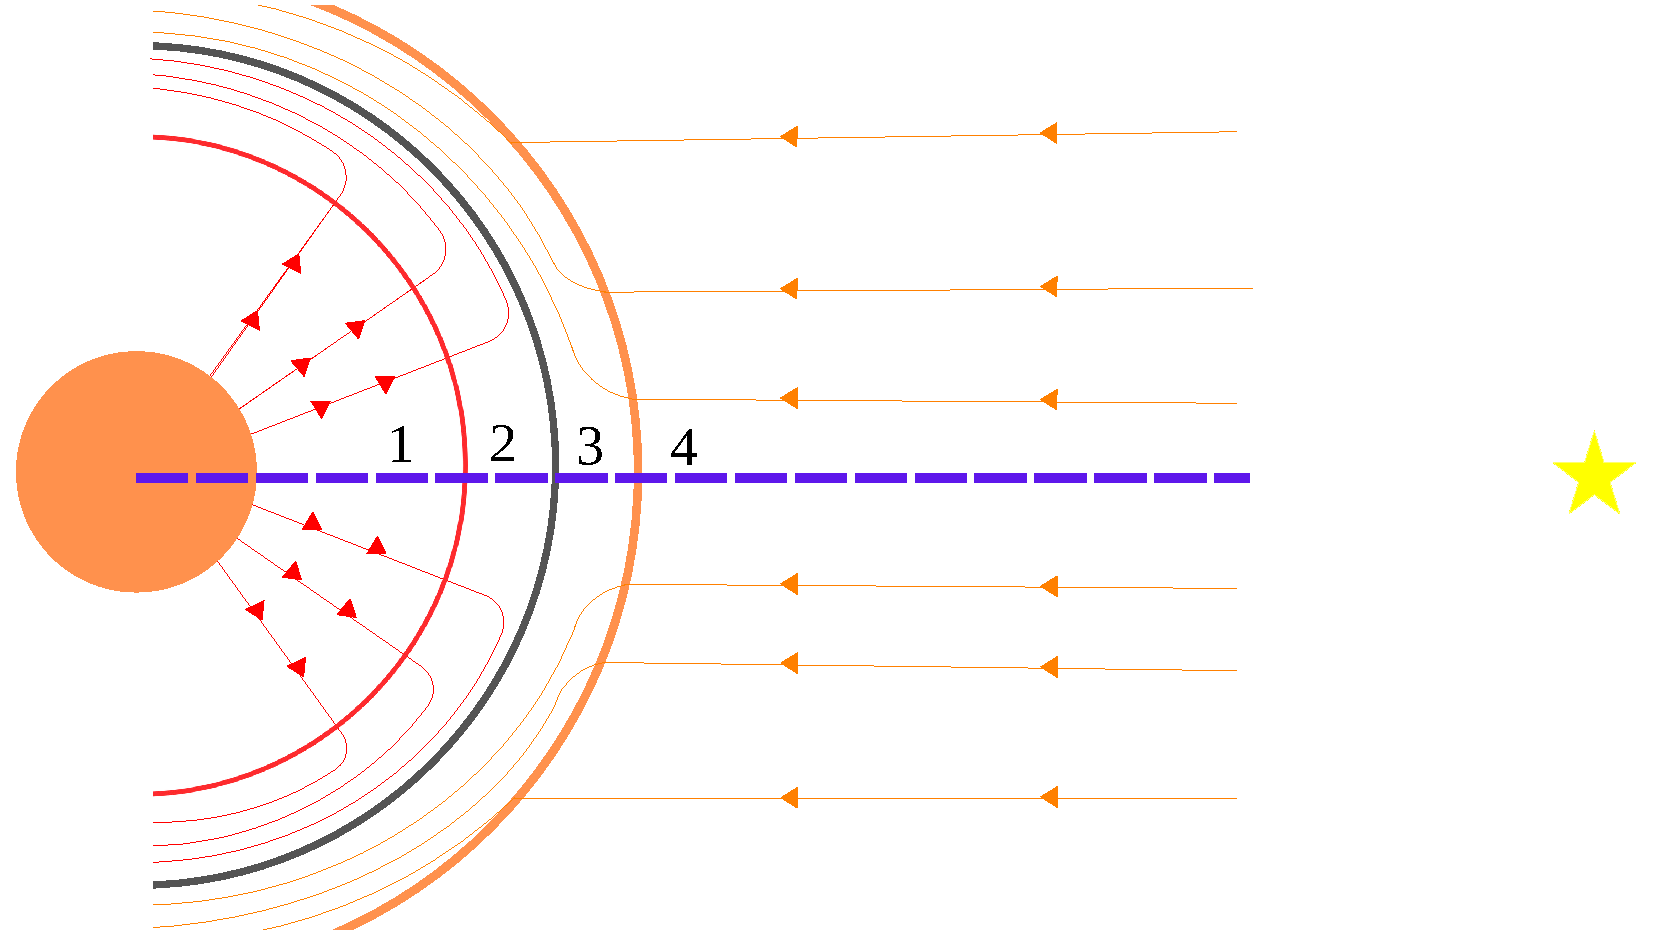
\includegraphics[width=\textwidth]{imagenes_corregidas/Arreglo 01.pdf}
%     \caption{La interacción entre el flujo fotoevaporativo y el viento
%       estelar de una estrella forma 4 zonas. El círculo naranja es el
%       glóbulo. La línea punteada azul que une el centro del glóbulo
%       con el centro de la estrella es el eje de simetría que vamos a
%       considerar en el modelo, la estrella se localiza en el otro
%       extremo de la línea punteada. Vemos como en este eje de simetría
%       tanto el viento estelar (líneas naranjas) como la radiación
%       inciden de forma perpendicular a la base del glóbulo y en
%       dirección contraria viaja el flujo fotoevaporativo (líneas
%       rojas). La zona 1 es donde el flujo fotoevaporativo sale de la
%       superficie del glóbulo con un número de Mach igual a 1 y va
%       aumentando. La zona 2 es el flujo fotoevaporativo chocado con el
%       viento estelar, la cual esperamos ver en las observaciones como
%       una cáscara y nos vamos a referir a ella como la cáscara
%       chocada. La zona 3 es el viento estelar chocado con el flujo
%       fotoevaporativo y la zona 4 es donde viaja el viento estelar
%       supersónico, el cual es menos denso que el flujo
%       fotoevaporativo. La discontinuidad de contacto se da entre las
%       zonas 2 y 3, la línea gris.}
%     \label{fig:zones}
% \end{figure}

% \begin{figure}[htb]
%     \centering    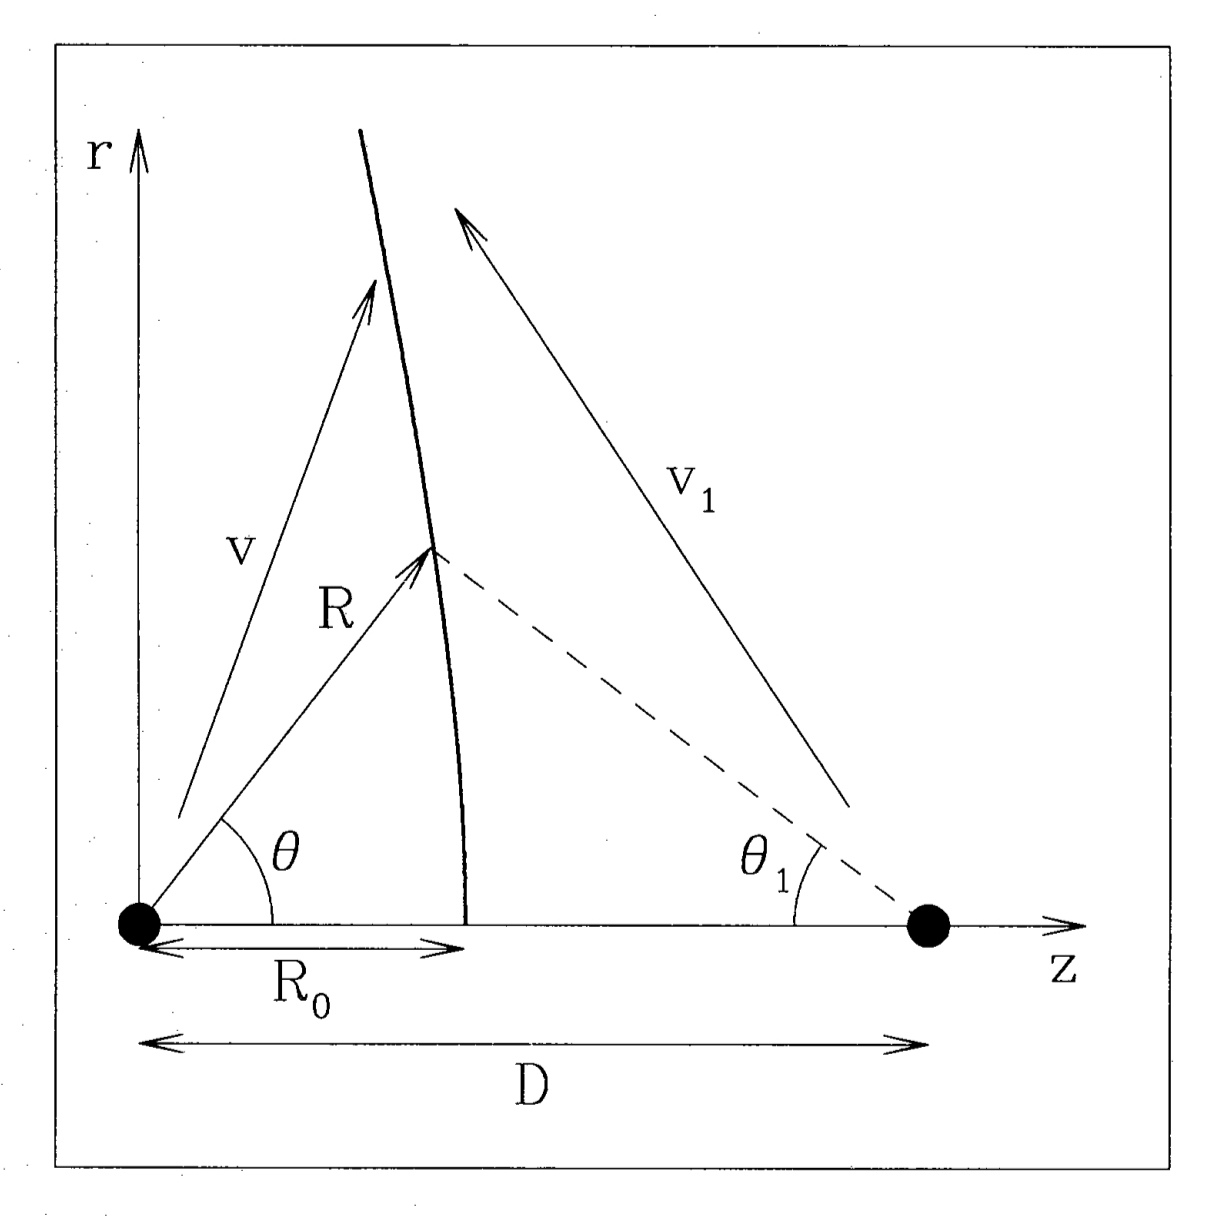
\includegraphics[width=0.8\textwidth]{images Chapter 2/C2_Canto.jpg}
%     \caption{Interacción de dos flujos supersónicos las cuales son
%       producidas por dos fuentes (puntos negro en el eje z) a una
%       distancia $D$. En esta interacción se produce una cáscara
%       delgada $R(\theta)$ cuando los flujos llegan a un equilibrio. Para
%       este problema se considera simetría cilíndrica
%       \citep{Canto:1996}.}
%     \label{fig:Canto1}
% \end{figure}

% \begin{figure}[htb]
%     \centering    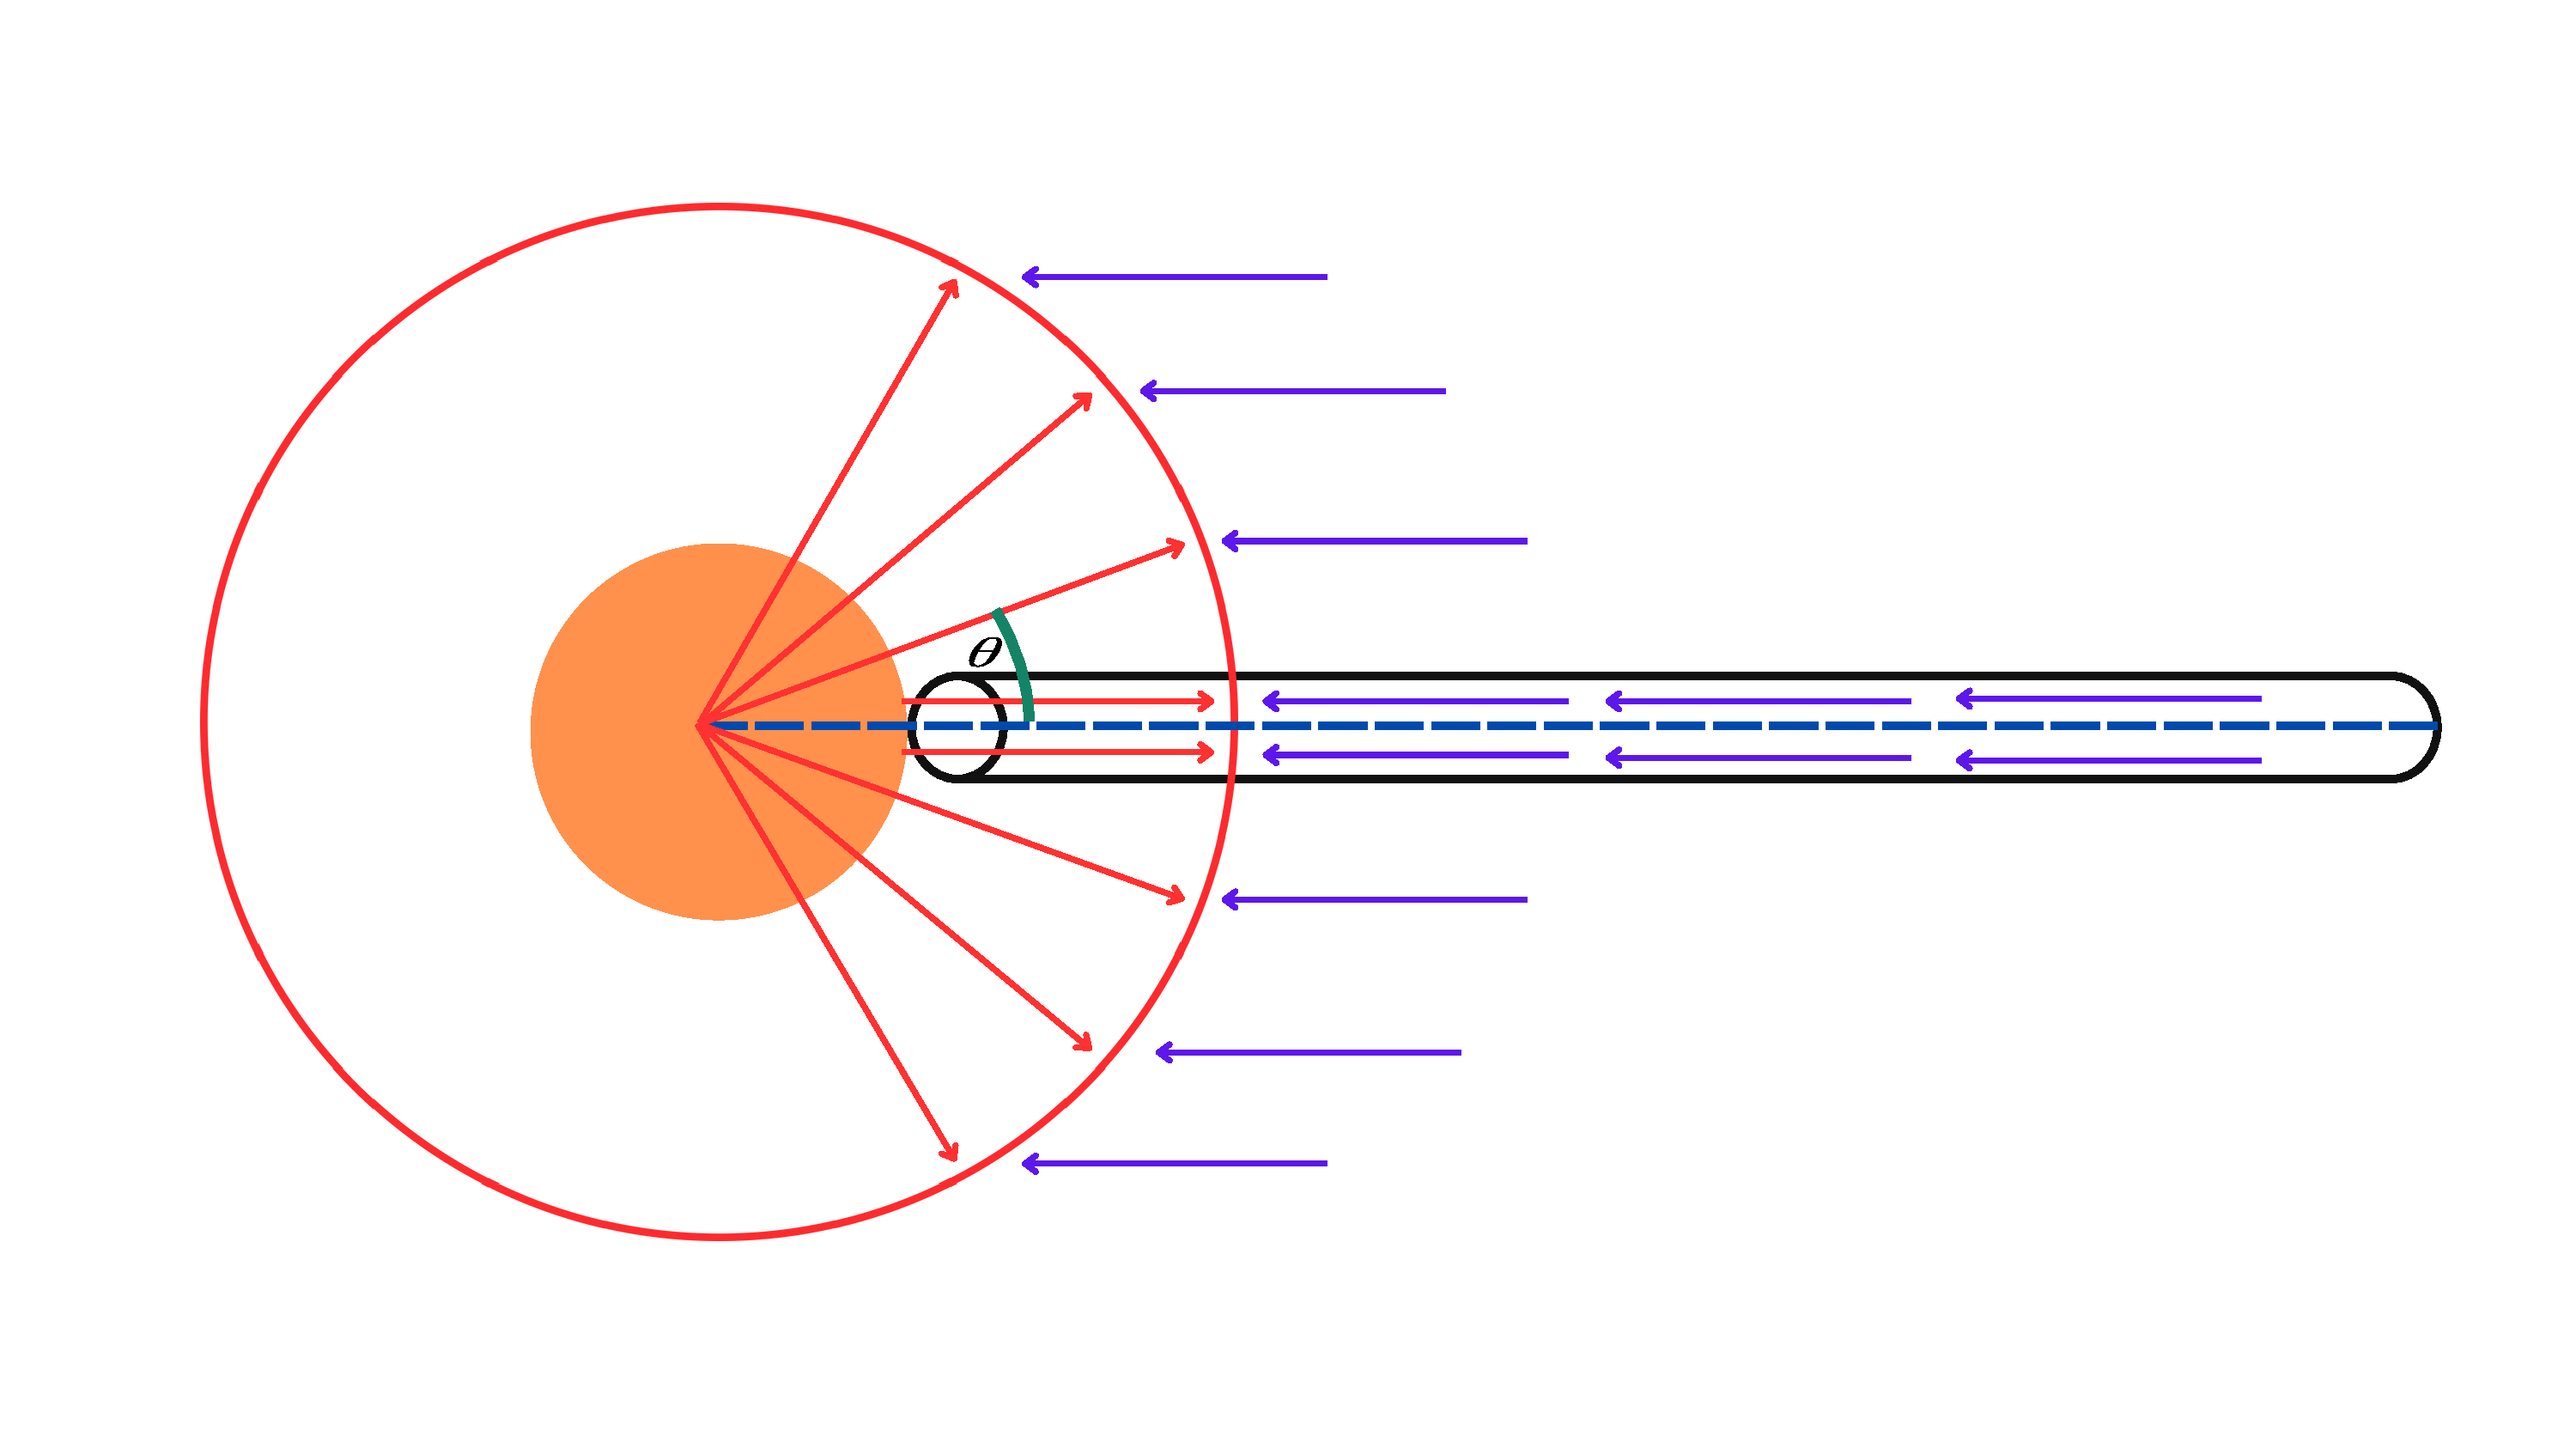
\includegraphics[width=\textwidth]{artesanales/ImgFi01-2.pdf}
%     \caption{La radiación y el viento estelar viajan hacia el glóbulo
%       como lo indican las flechas azules y vemos que inciden de manera
%       perpendicular a la superficie del glóbulo en el eje de simetría.
%       Mientras que el flujo fotoevaporativo por parte del glóbulo
%       viaja como lo indican las flechas rojas, y por lo tanto en la
%       interacción entre este flujo fotoevaporativo y el viento estelar
%       debemos considerar cierto ángulo si no estamos en el eje de
%       simetría.}
%     \label{fig:cilindross}
% \end{figure}

% \cite{Canto:1996} trata de una manera más detallada la interacción
% entre dos flujos hipersónicos en la cual considera dos fuentes
% separadas a una distancia $D$. En este análisis suponen que se forma
% una cáscara delgada cuando estos dos flujos llegan a un equilibrio de
% presiones como se puede ver en la Figura \ref{fig:Canto1}. En nuestro
% caso también esperamos que la zona 2 de la Figura \ref{fig:zones} sea
% delgada \citep{Wil:2019}.

% \section{Modelo hidrodinámico estacionario}

% Para nuestro modelo es importante mencionar que no estamos
% considerando ninguna fuerza de gravedad por parte de la estrella o del
% mismo glóbulo, así como tampoco ninguna otra fuerza externa (ver
% Apéndice \ref{App:fuerzas}). Vamos a considerar que solo el glóbulo
% está dominado por un campo magnético, mientras que para el gas
% ionizado no vamos a considerar ningún campo magnético.

% Para este trabajo en particular solo vamos a considerar como presión
% externa la presión RAM del viento estelar por parte de la estrella WR
% 124. Tomando en cuenta que el tiempo en el que ocurren las fases
% mencionadas en la Sección \ref{Sec:fluijos fotoevaporativos} es muy
% corto comparado con el tiempo de interacción que hay entre el flujo
% fotoevaporativo y el viento estelar, vamos a suponer que la capa
% aislante producida por la radiación UV ya se ha formado y ahora
% estamos en equilibrio de ionización. Por lo que vamos a considerar
% este modelo como estacionario, es decir, que los tamaños del glóbulo y
% de la cáscara chocada los vamos a tomar como constantes ya que no
% cambiaran sus tamaños de manera significativa.

% En la Figura \ref{fig:cilindross} vemos que podemos simplificar este
% problema si ponemos un cilindro de radio pequeño alrededor del eje de
% simetría. En este cilindro podemos ignorar los movimientos
% transversales ya que los gradientes en estas direcciones son muy
% pequeños si los comparamos con los gradientes en la dirección axial.
% Alrededor del eje de simetría podemos ver como tanto la radiación UV y
% el viento estelar inciden de manera perpendicular a la base del
% glóbulo y viajan en dirección contraria el flujo fotoevaporativo por
% parte del glóbulo. Por lo que primero vamos a resolver este problema
% solo en el eje de simetría, ya que aquí se vuelve unidimensional. Más
% adelante vamos a considerar qué pasaría si resolvemos este problema
% considerando un ángulo $\theta$ con respecto al eje de simetría.

% \section{Ecuación de estado y equilibrio de ionización}

% Para este caso vamos a considerar que el gas que está interaccionando
% con el viento estelar de la estrella es un gas ideal, por lo que
% nuestra ecuación de estado será
% \begin{equation}
%     PV = Nk_\mathrm{B}T,
% \end{equation} 
% donde $P$ es la presión del gas, $V$ su volumen, $N$ es el número de
% partículas, $k_\mathrm{B}$ la constante de Boltzman y $T$ es la
% temperatura. De aquí tenemos que \begin{equation} P = nk_\mathrm{B}T =
%   \frac{\rho k_\mathrm{B} T}{\bar{m}}
% \end{equation}
% donde $n$ es la densidad numérica, $\rho$ la densidad de masa y
% $\bar{m}$ es la masa promedio de las partículas en el gas. En este
% caso estamos considerando que el gas contiene principalmente hidrógeno
% un $90\%$ de todo el gas y una pequeña fracción de helio, por lo que
% vamos a considerar una masa promedio de
% $\bar{m}=\frac{0.9 m_\mathrm{p}+0.1\times4m_\mathrm{p}}{2}\approx0.6
% m_{\mathrm{p}}$ en el gas ionizado.

% En este gas ideal vamos a tomar la velocidad del sonido isotérmica, la
% cual está dada por
% \begin{equation}
%     c_\mathrm{s}  = \sqrt{\frac{k_\mathrm{B} T}{\bar{m}}}
% \end{equation} 
% de esta manera vemos que la velocidad del sonido en el gas ionizado
% solo depende de su temperatura. En este tipo de gases la velocidad del
% sonido es típicamente del orden de \SI{e6}{cm.s^{-1}}.

% Considerando que todas las fases mencionadas en la Sección
% \ref{Sec:fluijos fotoevaporativos} ya han sucedido, por lo que vamos a
% considerar que el flujo incidente de fotones ionizantes, $F_0$ está en
% equilibrio con las recombinaciones por unidad de área
% \begin{equation}
%     F_0 = n_\mathrm{e}n_\mathrm{i}h_1\alpha_\mathrm{B}
% \end{equation} 
% donde $h_1$ es la anchura efectiva y $\alpha_\mathrm{B}$ es el coeficiente
% de recombinación para el caso B (ver Apéndice \ref{App : tasa de
%   fotoionizacion}). Este coeficiente de recombinación para el caso B
% toma en cuenta las recombinaciones a todos los niveles, excepto al
% nivel base, esto ya que el fotón liberado en esta recombinación puede
% volver a ionizar algún otro átomo que se encuentre muy cerca
% \citep{Dyson:book:1980}.

\chapter{Analytical models of photoevaporative flows interacting
  with an external pressure}
\chaptermark{Analytical model}\label{Chapter : Modelo}

In this chapter we describe the model proposed to explain the
interaction between the photoevaporative flow from a globule and an
external pressure. This external pressure can be exerted by the very
same star that is photoevaporating the globule. In principle, the
model can be applied to any kind of globule like those mentioned in
Chapter \ref{Capitulo 1:introduccion}.

In this work we focus on the interaction between the globules’
photoevaporative flow\footnote{For simplicity we will refer to the
knots in the nebula as globules.} in the M1-67 nebula and the RAM
pressure of the stellar wind from the star WR~124. In Chapter
\ref{Chapter : 3} we will discuss in more detail how we identified
these globules in the M1-67 nebula; for now, we concentrate solely on
the model.

For this purpose, we assume that all the phases described in Section
\ref{Sec:fluijos fotoevaporativos} have already taken place and that
the system is now in ionization equilibrium. For simplicity, the
globule is taken to be spherical in this model.

In the interaction between the (supersonic) photoevaporative flow and
the stellar wind, two shocked zones are produced, with a contact
discontinuity between them, as depicted in Figure \ref{fig:zones}. Of
these zones, we expect to observe only the shocked photoevaporative
flow and not the shocked stellar wind, since the latter is less dense,
non-radiative, and has a cooling length (zone 3) larger than the
interaction region (zone 2).

\begin{figure}[htb]
    \centering    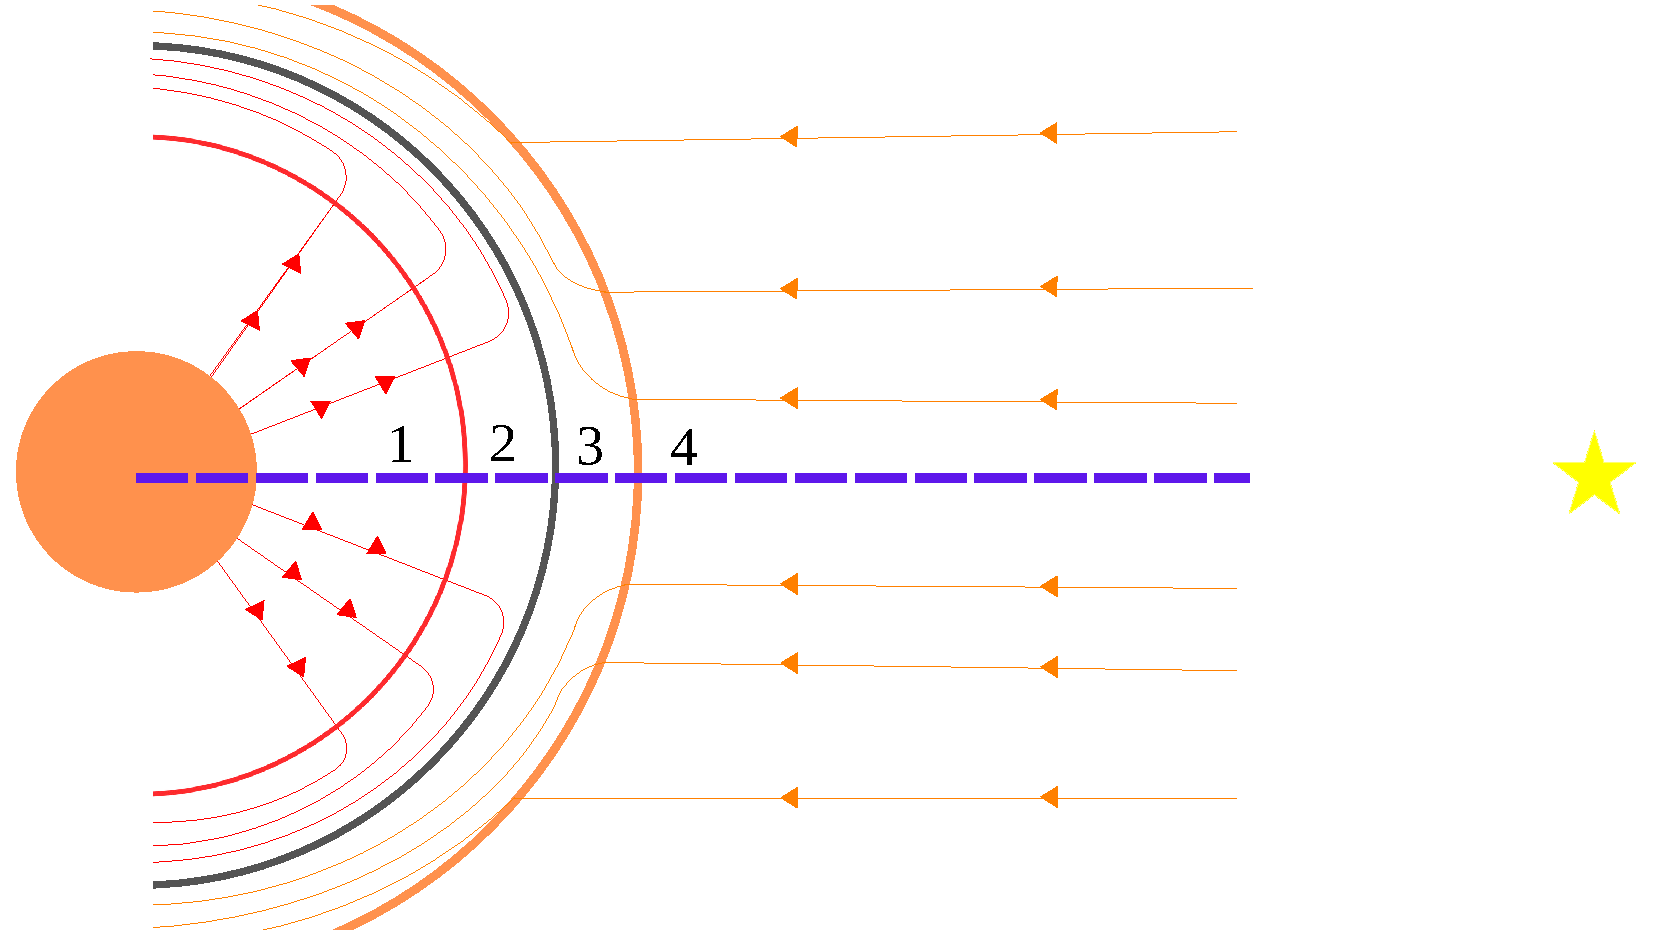
\includegraphics[width=\textwidth]{imagenes_corregidas/Arreglo 01.pdf}
    \caption{The interaction between the photoevaporative flow and the
      stellar wind of a star forms four zones. The orange circle is
      the globule. The blue dashed line joining the center of the
      globule to the center of the star is the symmetry axis adopted
      in the model; the star lies at the opposite end of the dashed
      line. Along this symmetry axis both the stellar wind (orange
      lines) and the radiation strike the base of the globule
      perpendicularly, while the photoevaporative flow (red lines)
      travels in the opposite direction. Zone 1 is where the
      photoevaporative flow emerges from the surface of the globule
      with Mach number equal to 1 and then increases. Zone 2 is the
      photoevaporative flow shocked by the stellar wind, which we
      expect to observe as a shell and to which we refer as the
      shocked shell. Zone 3 is the stellar wind shocked by the
      photoevaporative flow, and zone 4 is where the supersonic
      stellar wind travels, which is less dense than the
      photoevaporative flow. The contact discontinuity lies between
      zones 2 and 3 (gray line).}
    \label{fig:zones}
\end{figure}

\begin{figure}[htb]
    \centering    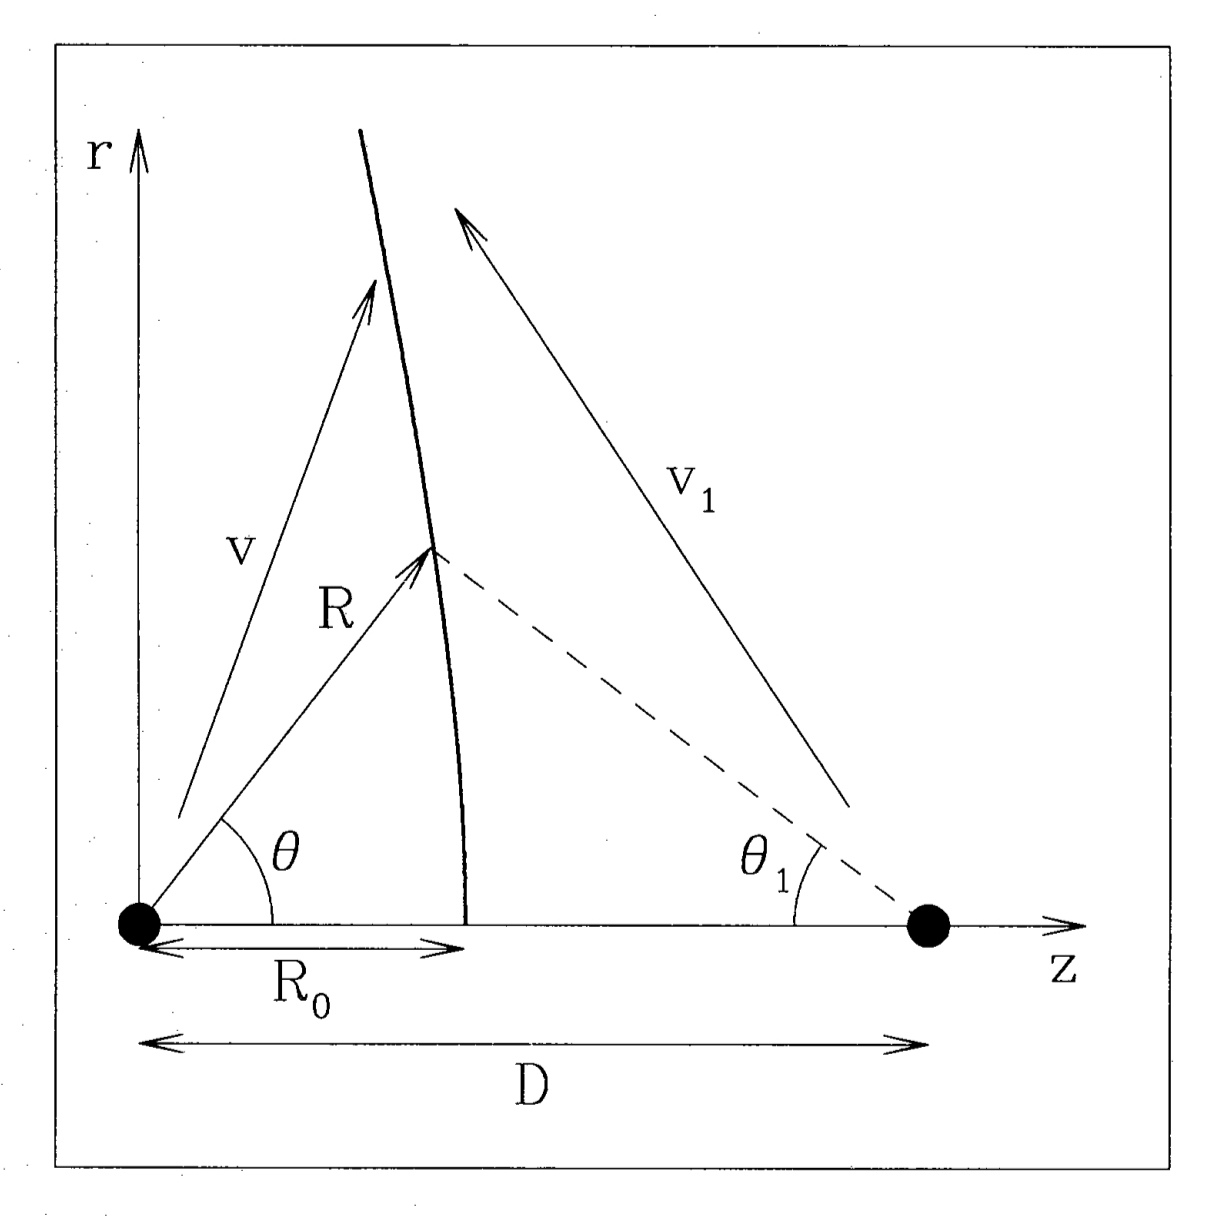
\includegraphics[width=0.8\textwidth]{images Chapter 2/C2_Canto.jpg}
    \caption{Interaction of two supersonic flows produced by two
      sources (black points on the $z$ axis) separated by a distance
      $D$. A thin shell $R(\theta)$ forms in this interaction when the
      flows reach equilibrium. Cylindrical symmetry is assumed for
      this problem \citep{Canto:1996}.}
    \label{fig:Canto1}
\end{figure}

\begin{figure}[htb]
    \centering    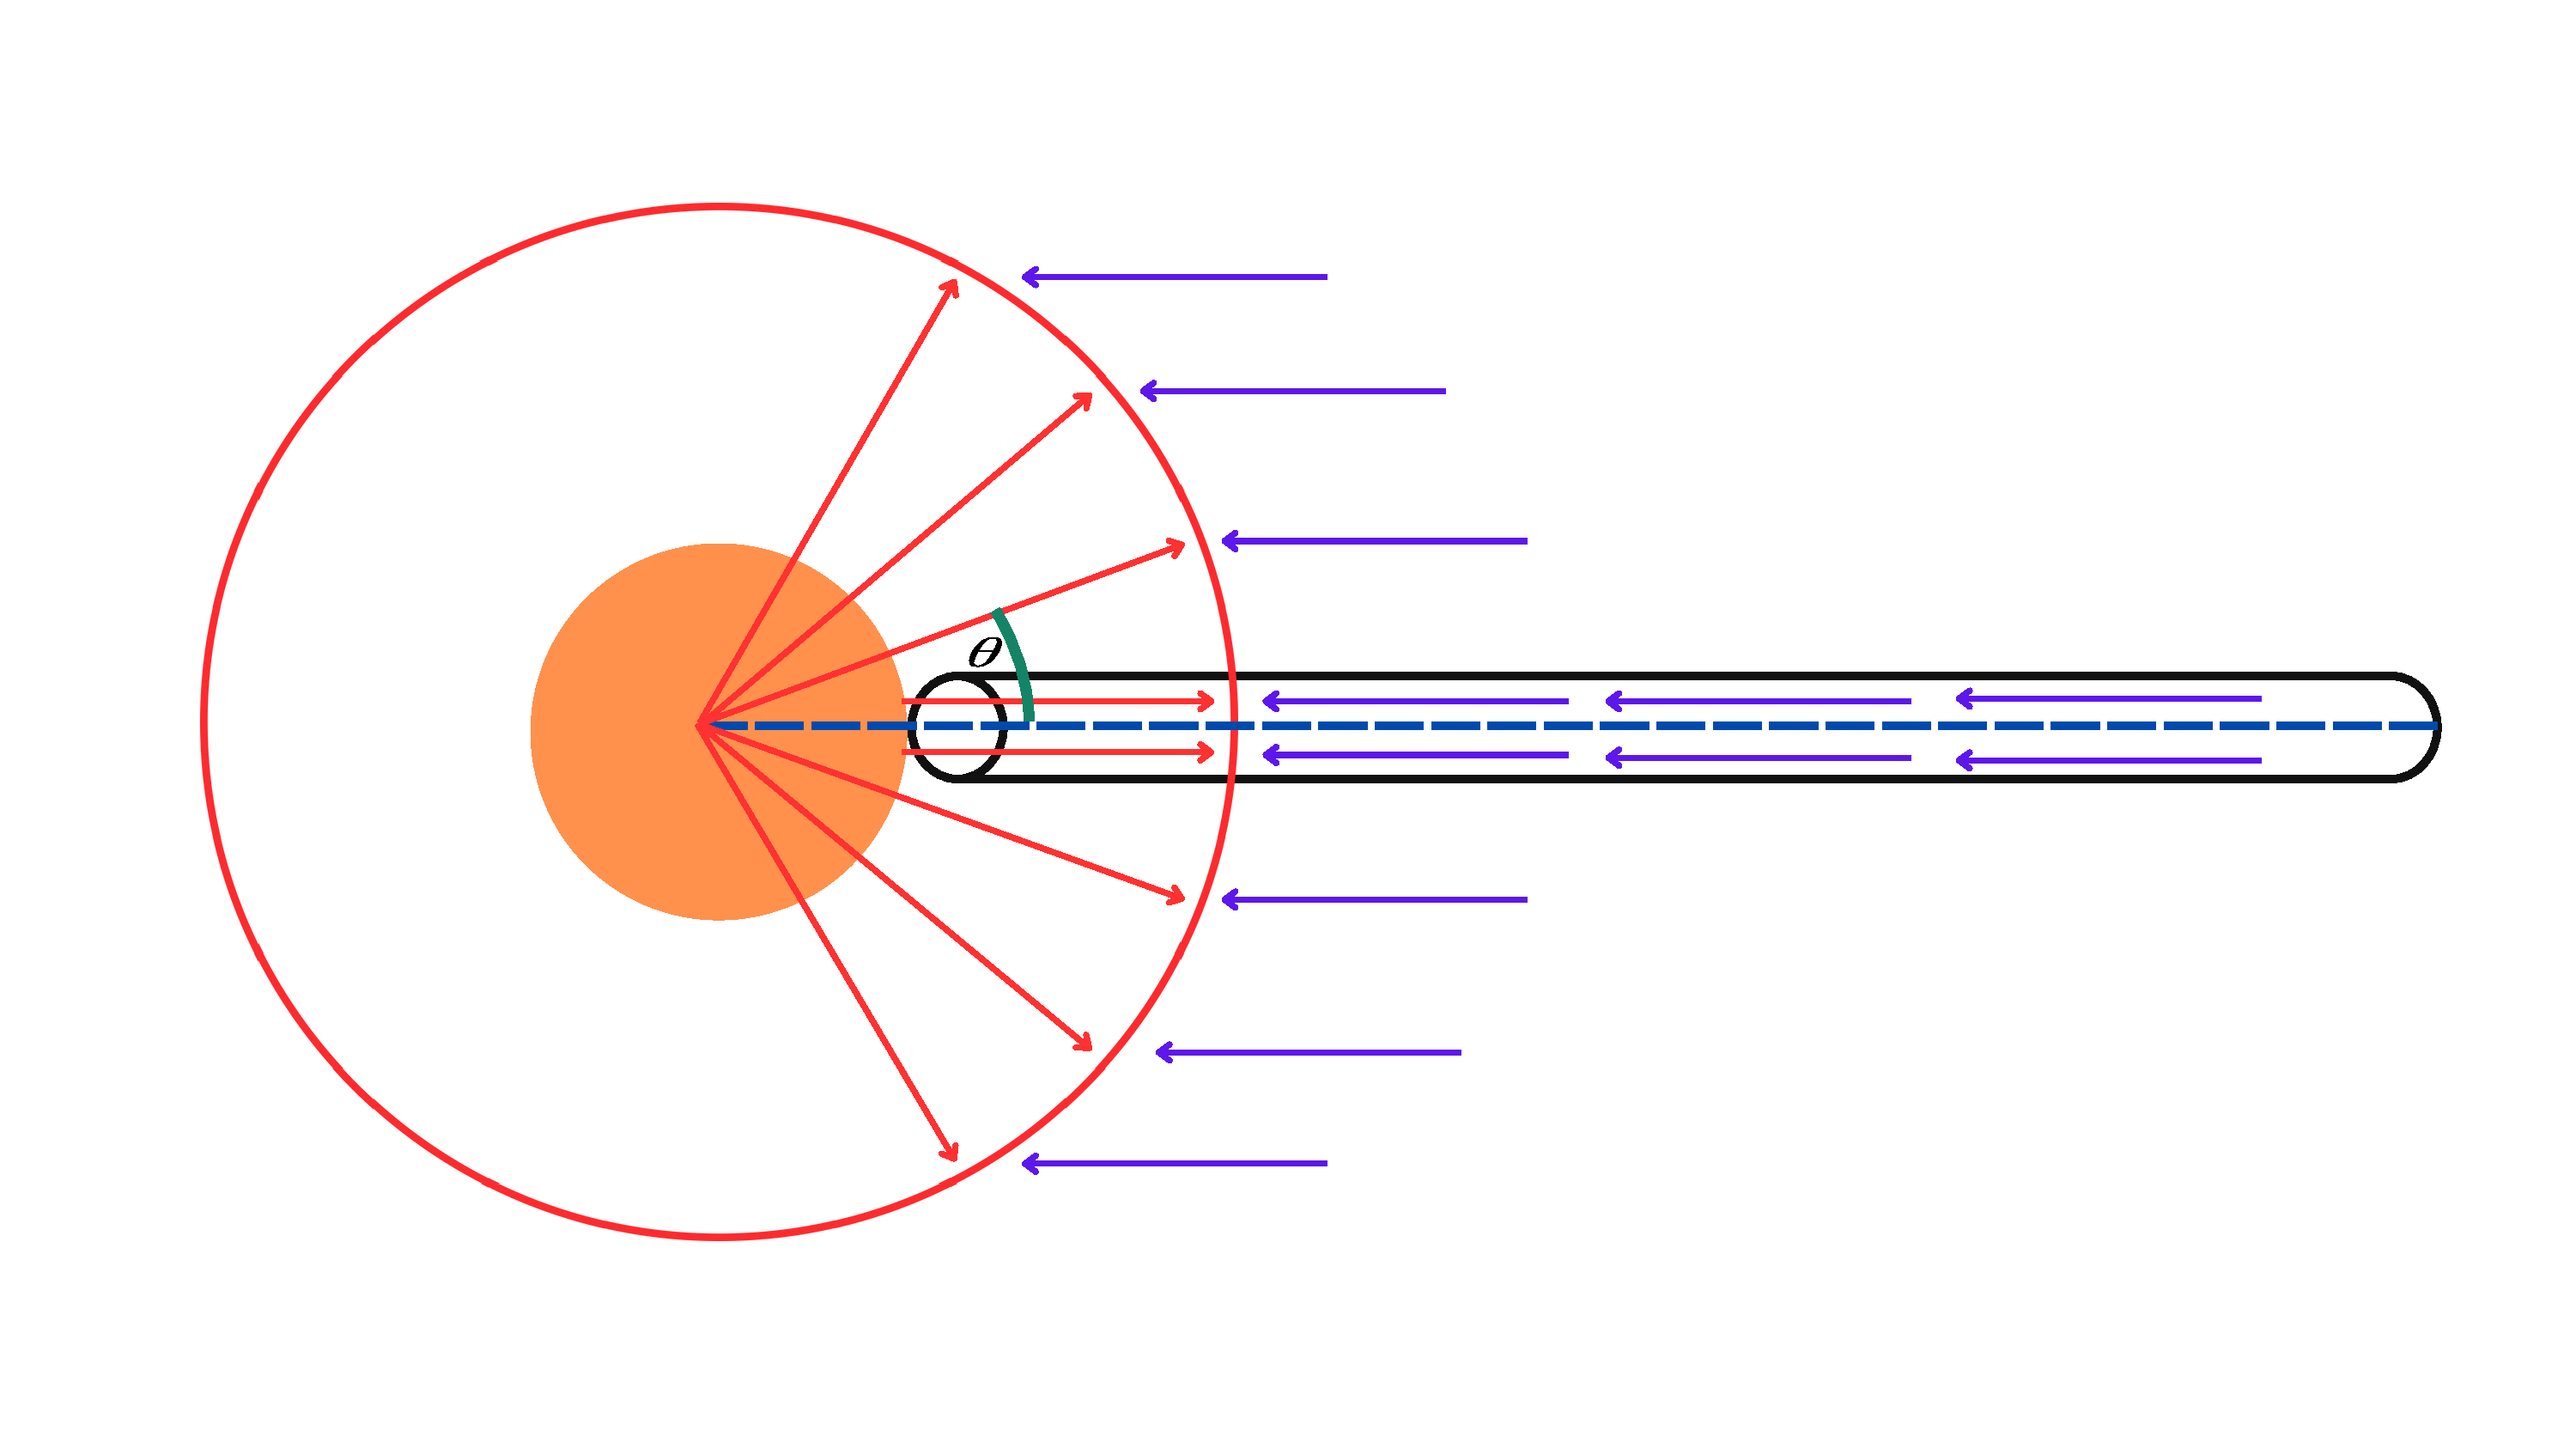
\includegraphics[width=\textwidth]{artesanales/ImgFi01-2.pdf}
    \caption{Radiation and stellar wind travel toward the globule as
      indicated by the blue arrows and strike the surface of the
      globule perpendicularly along the symmetry axis. The
      photoevaporative flow from the globule travels as shown by the
      red arrows; therefore, away from the symmetry axis the
      interaction between this photoevaporative flow and the stellar
      wind must be considered at a finite angle.}
    \label{fig:cilindross}
\end{figure}

\cite{Canto:1996} treat in greater detail the interaction between two
hypersonic flows produced by two sources separated by a distance $D$.
In their analysis they assume that a thin shell forms when these two
flows reach pressure equilibrium, as shown in Figure \ref{fig:Canto1}.
In our case we likewise expect zone 2 of Figure \ref{fig:zones} to be
thin \citep{Wil:2019}.

\section{Steady hydrodynamic model}

For our model it is important to note that we do not consider any
gravitational force from the star or from the globule itself, nor any
other external force (see Appendix \ref{App:fuerzas}). We assume that
only the globule is dominated by a magnetic field, while for the
ionized gas we neglect magnetic fields.

In this work we consider as the only external pressure the RAM
pressure of the stellar wind from WR~124. Given that the timescale for
the phases mentioned in Section \ref{Sec:fluijos fotoevaporativos} is
very short compared to the interaction timescale between the
photoevaporative flow and the stellar wind, we assume that the
insulating layer produced by the UV radiation has already formed and
that the system is now in ionization equilibrium. We therefore treat
the model as steady: the sizes of the globule and of the shocked shell
are taken as constant, since they will not change significantly.

Figure \ref{fig:cilindross} shows that we can simplify the problem by
placing a small-radius cylinder around the symmetry axis. Within this
cylinder we can ignore transverse motions, since gradients in those
directions are much smaller than the axial gradients. Near the symmetry
axis both the UV radiation and the stellar wind strike the base of the
globule perpendicularly, while the photoevaporative flow from the
globule travels in the opposite direction. We therefore first solve
the problem \emph{on the symmetry axis only}, where it becomes
one-dimensional. We then consider how the solution changes at an angle
$\theta$ with respect to the symmetry axis.

\section{Equation of state and ionization equilibrium}

In this case we take the gas interacting with the stellar wind to be
an ideal gas, so that our equation of state is
\begin{equation}
    PV = Nk_\mathrm{B}T,
\end{equation}
where $P$ is the gas pressure, $V$ its volume, $N$ the number of
particles, $k_\mathrm{B}$ Boltzmann’s constant, and $T$ the
temperature. From this we have
\begin{equation}
  P = nk_\mathrm{B}T = \frac{\rho k_\mathrm{B} T}{\bar{m}}
\end{equation}
where $n$ is the number density, $\rho$ the mass density, and
$\bar{m}$ the mean particle mass in the gas. Here we assume the gas is
composed mainly of hydrogen, $90\%$ of the total, with a small
fraction of helium, so we adopt a mean mass
$\bar{m}=\frac{0.9 m_\mathrm{p}+0.1\times4m_\mathrm{p}}{2}\approx0.6
m_{\mathrm{p}}$ in the ionized gas.

For this ideal gas we take the isothermal sound speed,
\begin{equation}
    c_\mathrm{s}  = \sqrt{\frac{k_\mathrm{B} T}{\bar{m}}},
\end{equation}
so the sound speed in the ionized gas depends only on its temperature.
In such gases the sound speed is typically of order
\SI{e6}{cm.s^{-1}}.

Since all the phases mentioned in Section
\ref{Sec:fluijos fotoevaporativos} have already occurred, we assume
that the incident flux of ionizing photons, $F_0$, is in equilibrium
with the recombinations per unit area,
\begin{equation}
    F_0 = n_\mathrm{e}n_\mathrm{i}h_1\alpha_\mathrm{B},
\end{equation}
where $h_1$ is the effective thickness and $\alpha_\mathrm{B}$ is the
case-B recombination coefficient (see Appendix \ref{App : tasa de
  fotoionizacion}). This case-B recombination coefficient accounts for
recombinations to all levels except the ground state, since the photon
emitted in such a recombination can reionize a nearby atom
\citep{Dyson:book:1980}.

% \section{Estructura del flujo fotoevaporativo}\label{Estructura}

% En este modelo estamos considerando un frente de ionización D-crítico
% \citep{Shuu:1992}, esto es, dentro del glóbulo vamos a tener una
% expansión subsónica del gas desde el punto de vista del frente de
% ionización y una expansión supersónica en el gas ionizado desde el
% punto de vista del frente de ionización, por lo que tendremos un punto
% sónico el cual está justo detrás del frente de ionización. En este
% caso por simplicidad vamos a considerar el frente de ionización como
% una discontinuidad en el que pasamos de tener gas no ionizado a tener
% un gas totalmente ionizado, por lo que tomaremos que el punto sónico
% se da justo en $r_0$, que es el radio del glóbulo (ver Figura
% \ref{fig:parameters}). Así que vamos a considerar que el gas tiene un
% número de Mach igual a 1 en $r_0$ y este va a ir aumentando conforme
% atraviesa toda la zona 1 de la Figura \ref{fig:zones} ya que se va
% expandiendo libremente. En principio podríamos considerar que tanto el
% radio del glóbulo como la densidad en su superficie son parámetros
% libres, pero con las observaciones podemos medir el radio y la
% densidad la podemos calcular ya que esta debe ser consistente por
% haber considerado equilibrio de ionización.

% Con este modelo se pretende ver hasta donde llegamos a un equilibrio
% de presión entre la presión por parte del flujo fotoevaporativo y la
% presión RAM del viento estelar. Para el caso de la presión del flujo
% fotoevaporativo vamos a considerar tanto la presión térmica como la
% hidrodinámica, por lo que la presión total en la base del glóbulo está
% dada por
% \begin{equation}\label{eq: Presion total}
%     P_\mathrm{tot}=P_\mathrm{ter}+P_\mathrm{hid}=n\bar{m}c_\mathrm{s}^2+n\bar{m}u^2=\rho c_\mathrm{s}^2(1+M^2),
% \end{equation}
% donde $u$ es la velocidad del gas en la parte ionizada y $M$ es el
% número de Mach.

% \begin{figure}[htb]
%     \centering 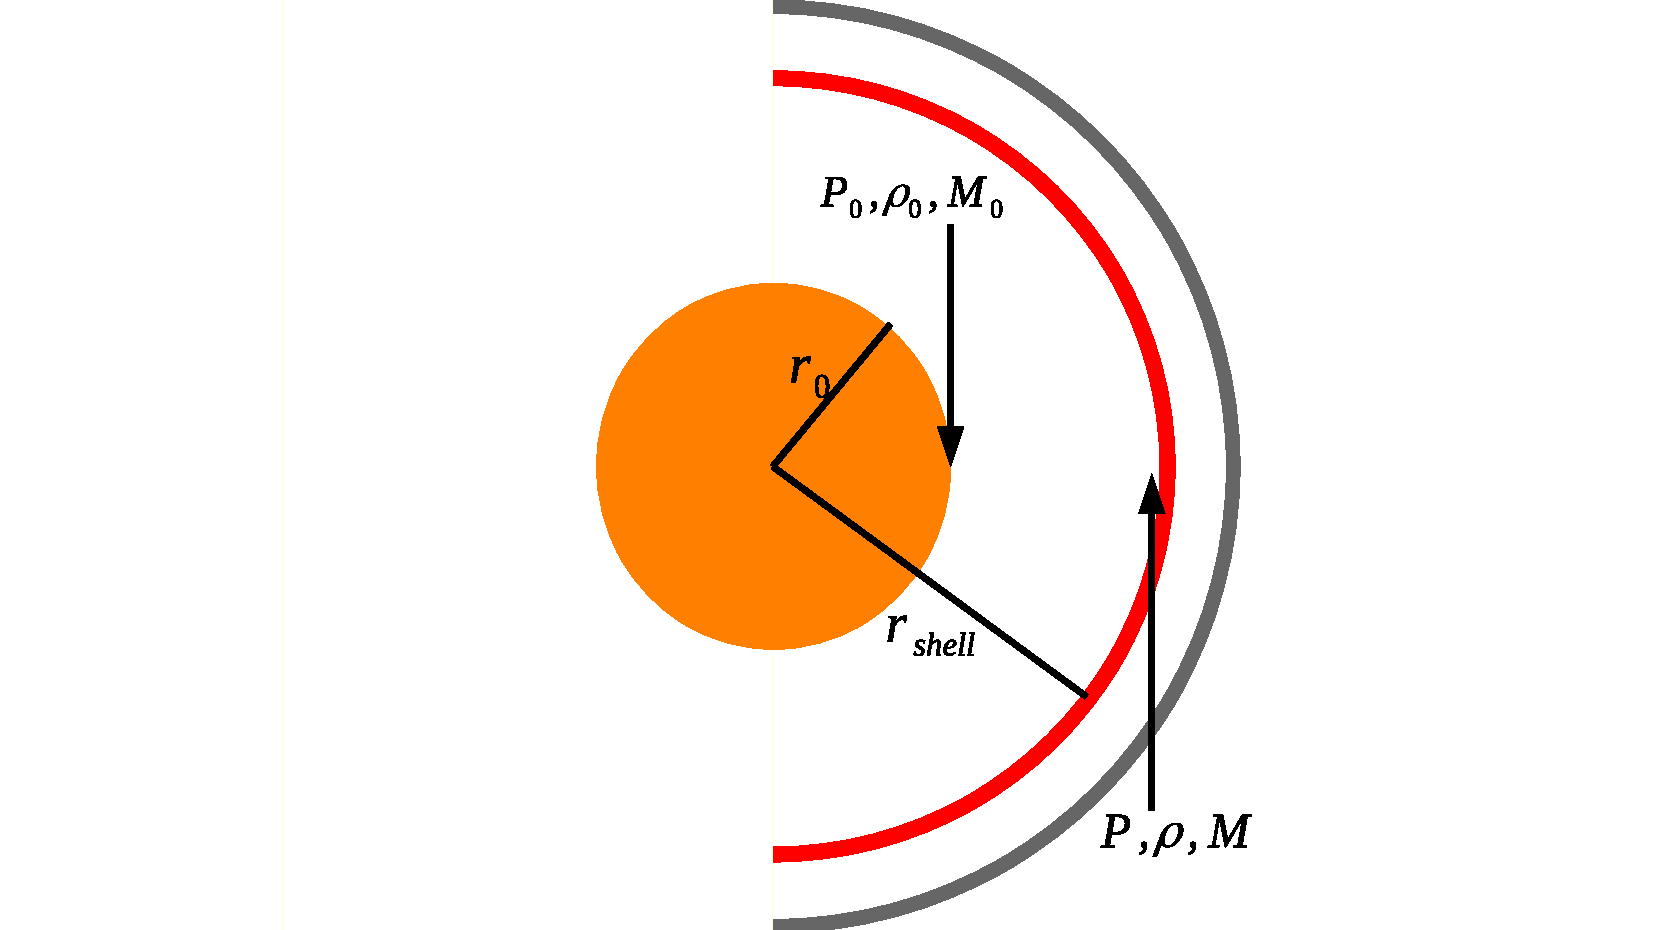
\includegraphics[width=\textwidth]{imagenes_corregidas/Arreglo 02_n.pdf}
%     \caption{En este diagrama esquemático $r_0$ es el radio del
%       glóbulo neutro, mientras que $\rho_0,M_0$ y $P_0$ son los valores
%       que tenemos en la superficie del glóbulo y varían con dirección
%       a la estrella hasta tener diferentes valores en
%       $r_\mathrm{shell}$, que es el radio del centro del glóbulo hasta
%       la base del flujo fotoevaporativo chocado, $\rho,M$ y $P$ son los
%       valores que tendrán en la base del flujo fotoevaporativo
%       chocado.}
%     \label{fig:parameters}
% \end{figure}

% Este equilibrio de presión se logrará a un radio $r_\mathrm{shell}$
% que es donde la presión del flujo fotoevaporativo ha disminuido una
% fracción $f$ de lo que era la presión inicial. Por lo que la presión
% cambia como
% \begin{equation}\label{eq : 1}
% f=\frac{P}{P_0}=\frac{\rho c_\mathrm{s}^2(1+M^2)}{\rho_0 c_\mathrm{s}^2(1+1)}=\frac{\rho}{\rho_0}\frac{1+M^2}{2},
% \end{equation}
% donde $P_0$ es la presión en la base del glóbulo, recordemos que aquí
% estamos considerando el punto sónico, por lo que $M_0=1$. $P$ es la
% presión del flujo fotoevaporativo justo antes de $r_\mathrm{shell}$.
% Considerando la ecuación para la conservación de masa tenemos que
% \begin{equation}\label{eq : 2}
% \rho r^2M	=\rho_0 r_0^2.
% \end{equation}
% Finalmente, si consideramos la ecuación de Bernoulli isotérmica 
% \begin{equation}
% \frac{v^2}{2}+c_\mathrm{s}^2\ln\rho=\text{constante}
% \end{equation}
% en la Ecuación (\ref{eq: Presion total}) tenemos que \citep{Dyson:1968}
% \begin{equation}\label{eq ; 3} \frac{r}{r_0}=M^{-1/2}e^{\frac{M^2-1}{4}}.
% \end{equation}
% Combinando las ecuaciones (\ref{eq : 1}), (\ref{eq : 2}) y (\ref{eq ;
%   3}) tenemos la ecuación
% \begin{equation}
%     f=\frac{1+M^2}{2}exp\left(\frac{1-M^2}{2}\right),
% \end{equation}
% la cual solo depende de $M$ y podemos resolver de manera
% numérica\footnote{En nuestro caso usamos la función fsolve de la
%   paquetería scipy.optimize, la documentación se encuentra en
%   \url{https://docs.scipy.org/doc/scipy-1.12.0/reference/generated/scipy.optimize.fsolve.html}}
% dándole diferentes valores a $f$. Una vez que resolvemos esta ecuación
% podemos saber los valores de las incógnitas $\rho/\rho_0$ y $r/r_0$ usando
% las ecuaciones (\ref{eq : 2}) y (\ref{eq ; 3}). Obteniendo así, que
% tanto la presión como la densidad decaen con el radio, mientras que el
% número de Mach aumenta como vemos en la Figura \ref{fig:grafica_C2}.
% Cabe mencionar que la Figura \ref{fig:grafica_C2} se obtiene
% resolviendo las ecuaciones (\ref{eq : 1}), (\ref{eq : 2}) y (\ref{eq ;
%   3}) en el eje de simetría. Pero esto cambiaría si consideramos
% cierto ángulo $\theta\neq 0 $ ya que tanto la presión como la densidad escalan
% con el ángulo como $\cos^{1/2}\theta$, pero $M$ no \citep{Tarango:2018}.

% \begin{figure}[htb]
%     \centering    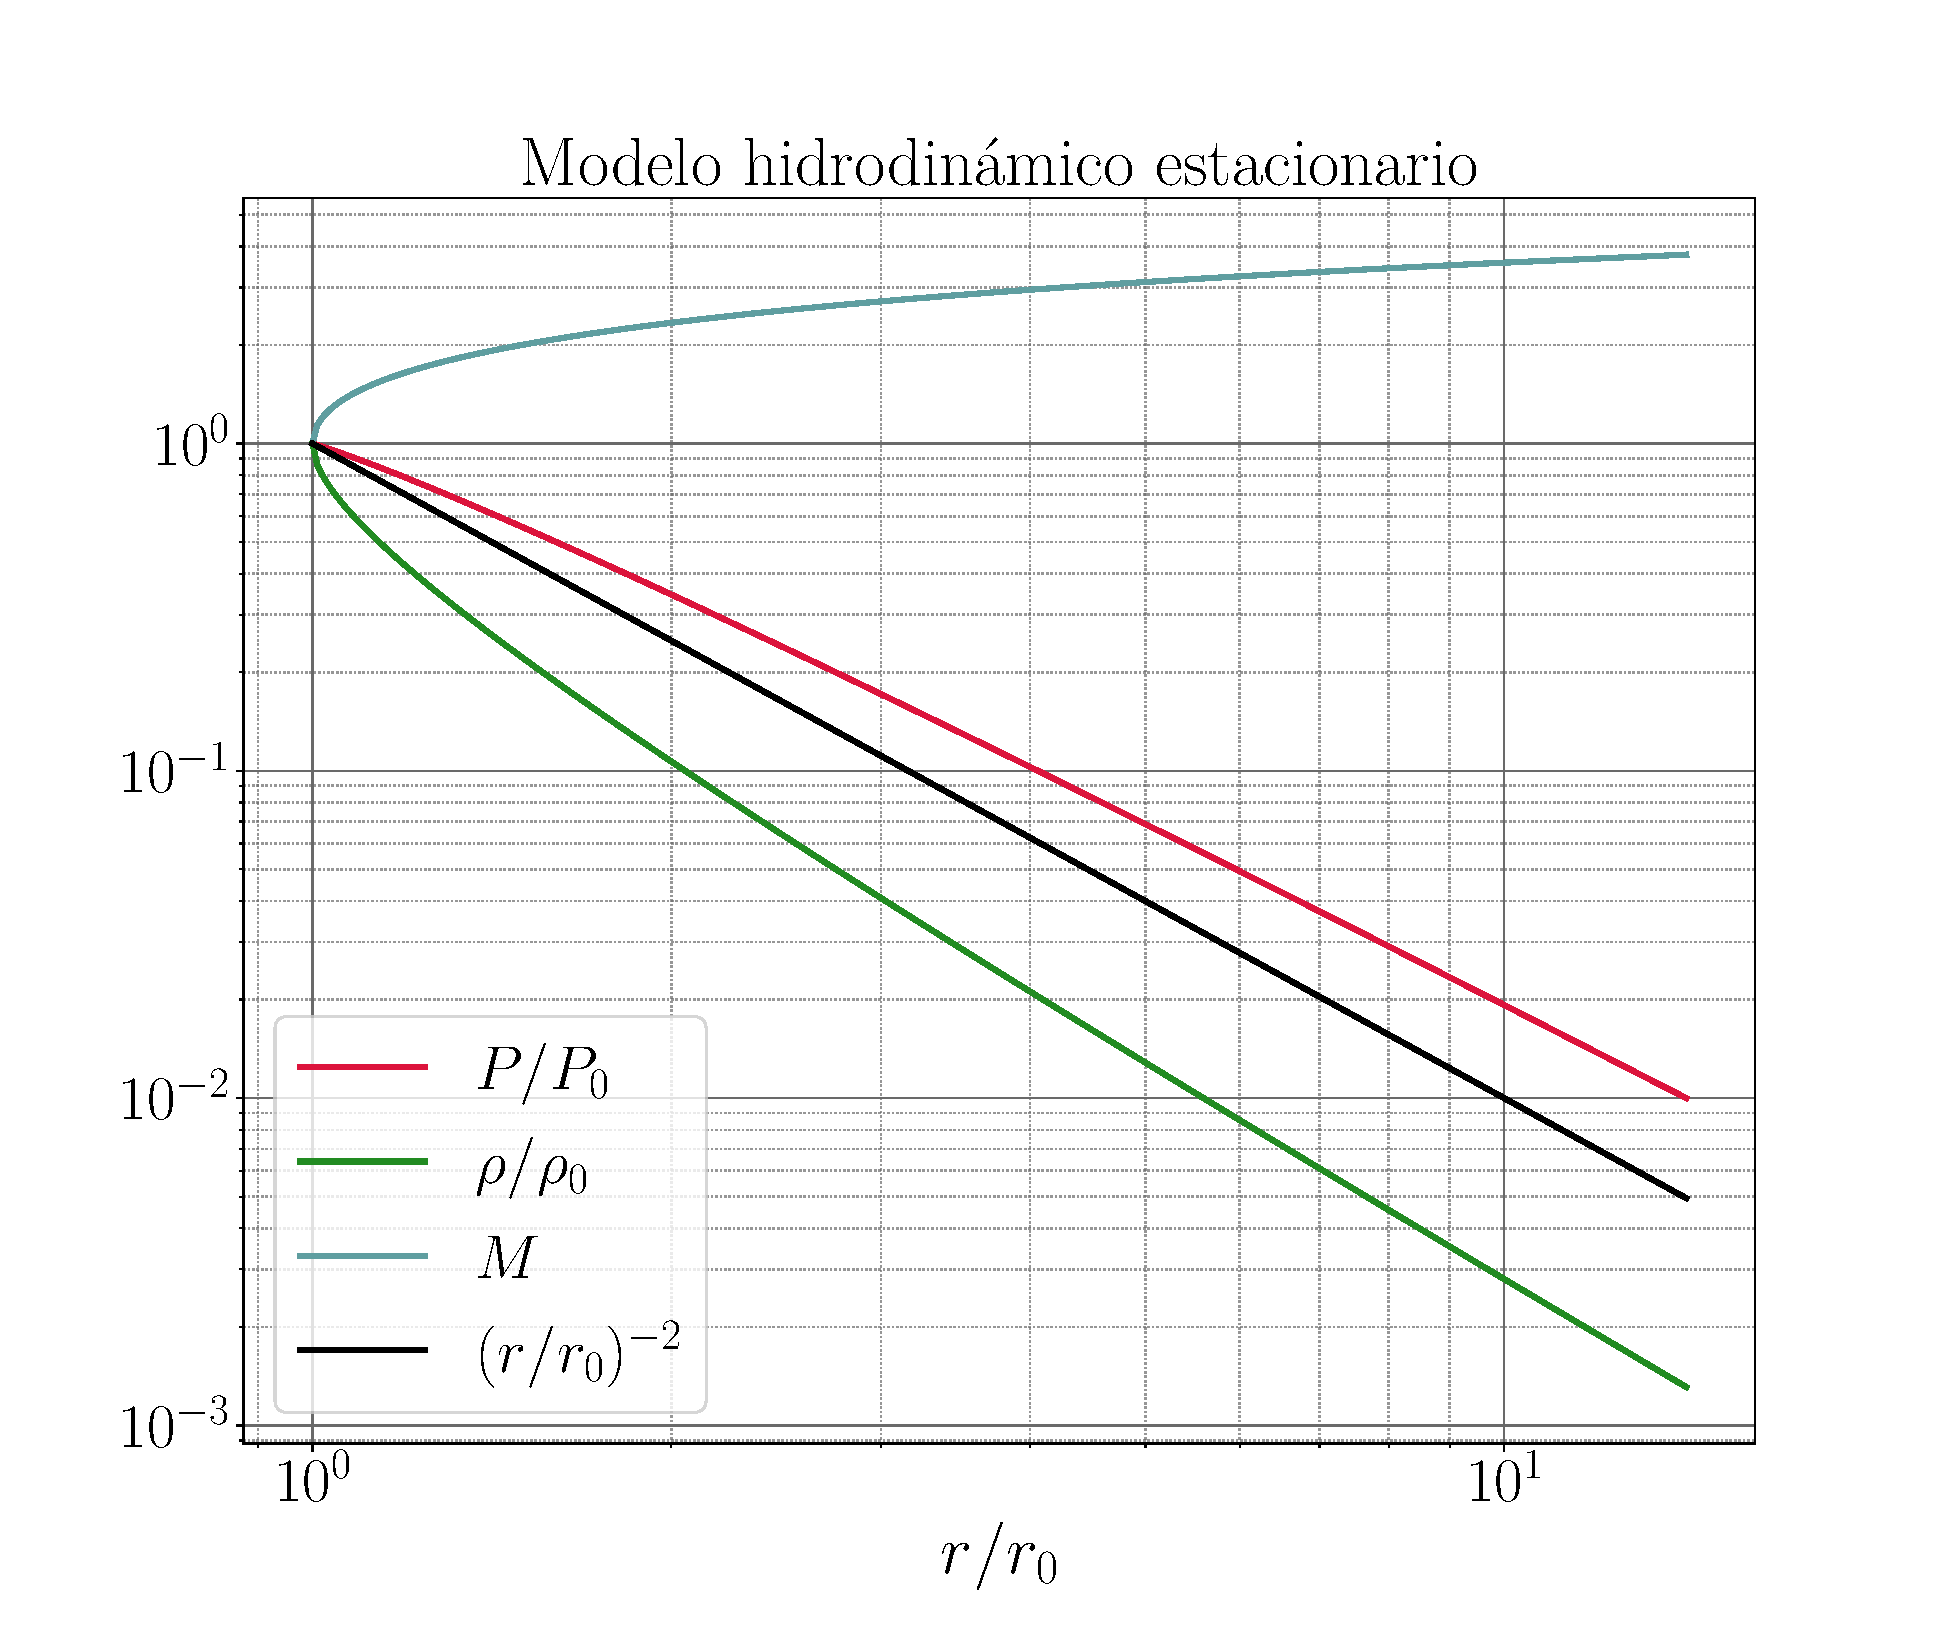
\includegraphics[width=\textwidth]{Nuevas imagenes finales/C2_estructura.pdf}
%     \caption{Gráfica del número de Mach $M$, densidad $\rho$ y la presión
%       total $P$ normalizados como función de $r/r_0$. También podemos
%       ver una caída que va como $\sim r^{-2}$ (línea negra). Podemos
%       notar que la densidad cae más rápido que $r^{-2}$, mientras que
%       la presión total cae más lento, en ambos casos se debe a la
%       aceleración del flujo. }
%     \label{fig:grafica_C2}
% \end{figure}

\section{Structure of the photoevaporative flow}\label{Estructura}

In this model we consider a D-critical ionization front
\citep{Shuu:1992}; that is, inside the globule there is a subsonic
expansion of the gas as seen from the ionization front, while in the
ionized gas there is a supersonic expansion as seen from the
ionization front. Consequently there is a sonic point located just
behind the ionization front. For simplicity we treat the ionization
front as a discontinuity across which the gas jumps from neutral to
fully ionized, and we therefore take the sonic point to occur exactly
at $r_0$, the radius of the globule (see Figure \ref{fig:parameters}).
Thus we assume the gas has Mach number equal to 1 at $r_0$, increasing
as it traverses zone 1 of Figure \ref{fig:zones} owing to free
expansion. In principle the globule radius and the density at its
surface could be taken as free parameters, but with the observations
we can measure the radius, and the density can be computed because it
must be consistent with our assumption of ionization equilibrium.

With this model we aim to determine where pressure balance is attained
between the pressure of the photoevaporative flow and the stellar-wind
RAM pressure. For the photoevaporative-flow pressure we include both
thermal and hydrodynamic terms, so that the total pressure at the base
of the globule is
\begin{equation}\label{eq: Presion total}
    P_\mathrm{tot}=P_\mathrm{ter}+P_\mathrm{hid}=n\bar{m}c_\mathrm{s}^2+n\bar{m}u^2=\rho c_\mathrm{s}^2(1+M^2),
\end{equation}
where $u$ is the velocity of the ionized gas and $M$ is the Mach
number.

\begin{figure}[htb]
    \centering 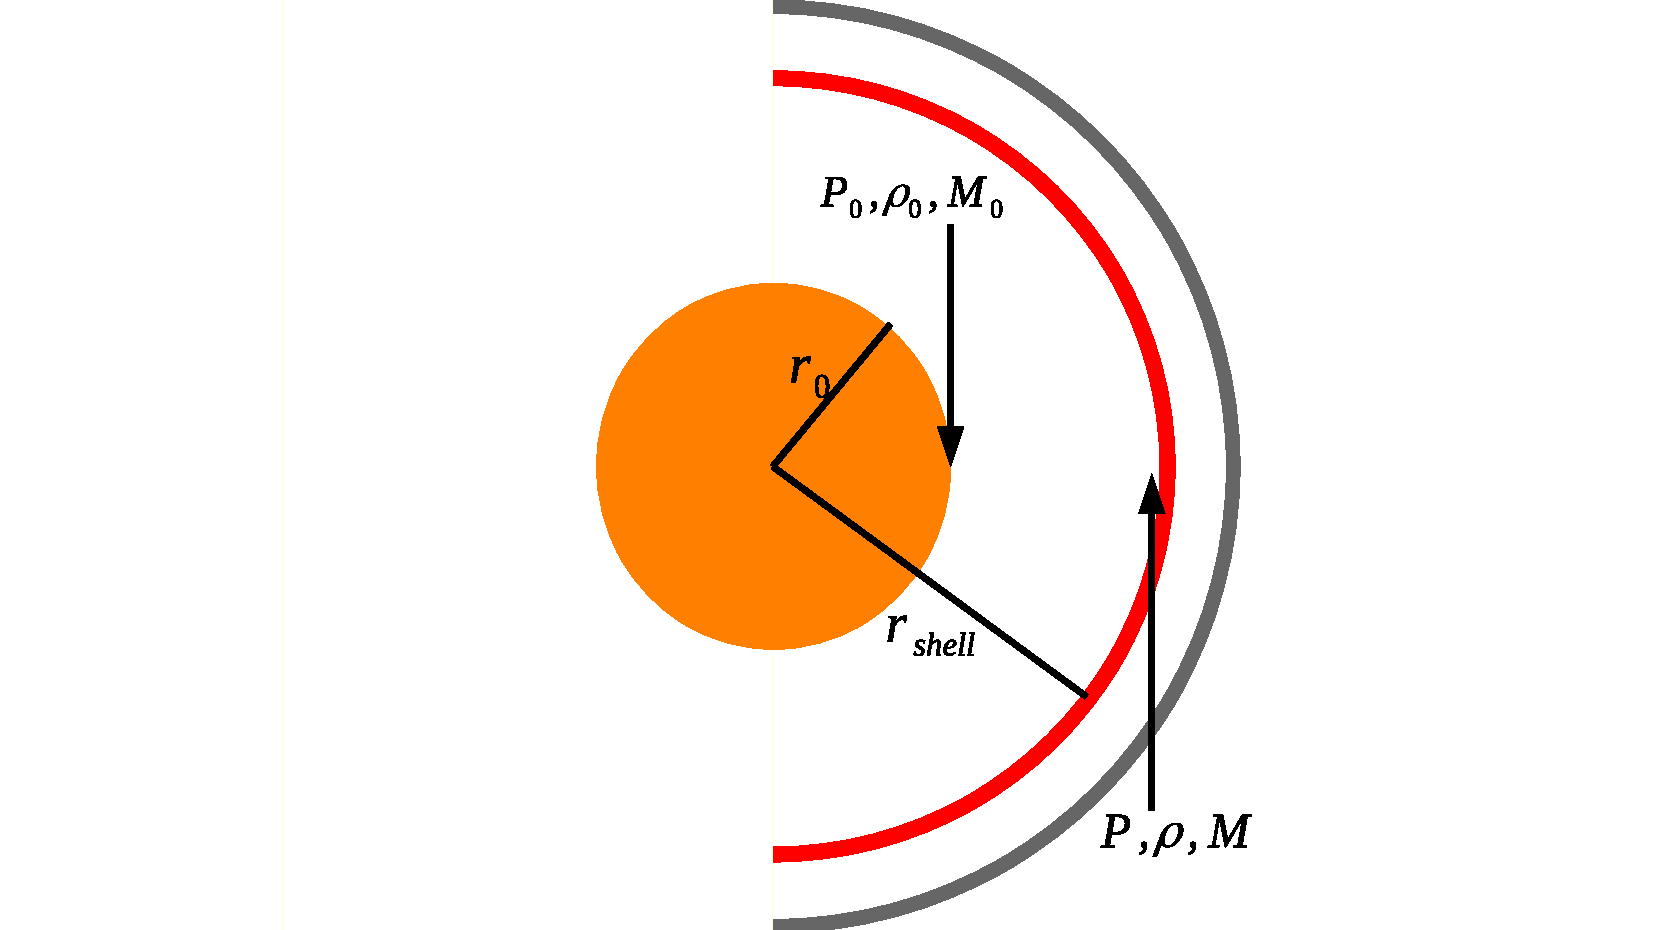
\includegraphics[width=\textwidth]{imagenes_corregidas/Arreglo 02_n.pdf}
    \caption{In this schematic, $r_0$ is the radius of the neutral
      globule, while $\rho_0$, $M_0$, and $P_0$ are the values at the
      globule surface, varying toward the star until they take on
      different values at $r_\mathrm{shell}$, the distance from the
      globule center to the base of the shocked photoevaporative flow.
      The quantities $\rho$, $M$, and $P$ are the corresponding values
      at the base of the shocked photoevaporative flow.}
    \label{fig:parameters}
\end{figure}

This pressure equilibrium is reached at a radius $r_\mathrm{shell}$,
where the pressure of the photoevaporative flow has dropped to a
fraction $f$ of its initial value. Hence the pressure varies as
\begin{equation}\label{eq : 1}
f=\frac{P}{P_0}=\frac{\rho c_\mathrm{s}^2(1+M^2)}{\rho_0 c_\mathrm{s}^2(1+1)}=\frac{\rho}{\rho_0}\frac{1+M^2}{2},
\end{equation}
where $P_0$ is the pressure at the base of the globule. Recall that we
are taking the sonic point there, so $M_0=1$. $P$ is the pressure of
the photoevaporative flow just upstream of $r_\mathrm{shell}$. From
mass conservation we have
\begin{equation}\label{eq : 2}
\rho r^2M	=\rho_0 r_0^2.
\end{equation}
Finally, adopting the isothermal Bernoulli equation,
\begin{equation}
\frac{v^2}{2}+c_\mathrm{s}^2\ln\rho=\text{constant},
\end{equation}
equation (\ref{eq: Presion total}) yields \citep{Dyson:1968}
\begin{equation}\label{eq ; 3} \frac{r}{r_0}=M^{-1/2}e^{\frac{M^2-1}{4}}.
\end{equation}
Combining equations (\ref{eq : 1}), (\ref{eq : 2}), and (\ref{eq ; 3})
we obtain
\begin{equation}
    f=\frac{1+M^2}{2}\,exp\left(\frac{1-M^2}{2}\right),
\end{equation}
which depends only on $M$ and can be solved numerically\footnote{In
  our case we use the function \texttt{fsolve} from
  \texttt{scipy.optimize}; see the documentation at
  \url{https://docs.scipy.org/doc/scipy-1.12.0/reference/generated/scipy.optimize.fsolve.html}.}
for different values of $f$. Once this equation is solved, the
unknowns $\rho/\rho_0$ and $r/r_0$ can be obtained from equations
(\ref{eq : 2}) and (\ref{eq ; 3}). In this way we find that both the
pressure and the density decrease with radius, while the Mach number
increases, as shown in Figure \ref{fig:grafica_C2}. Note that Figure
\ref{fig:grafica_C2} is obtained by solving equations (\ref{eq : 1}),
(\ref{eq : 2}), and (\ref{eq ; 3}) on the symmetry axis. This would
change if we consider a finite angle $\theta\neq 0$, since both the
pressure and the density scale with angle as $\cos^{1/2}\theta$,
whereas $M$ does not \citep{Tarango:2018}.

\begin{figure}[htb]
    \centering    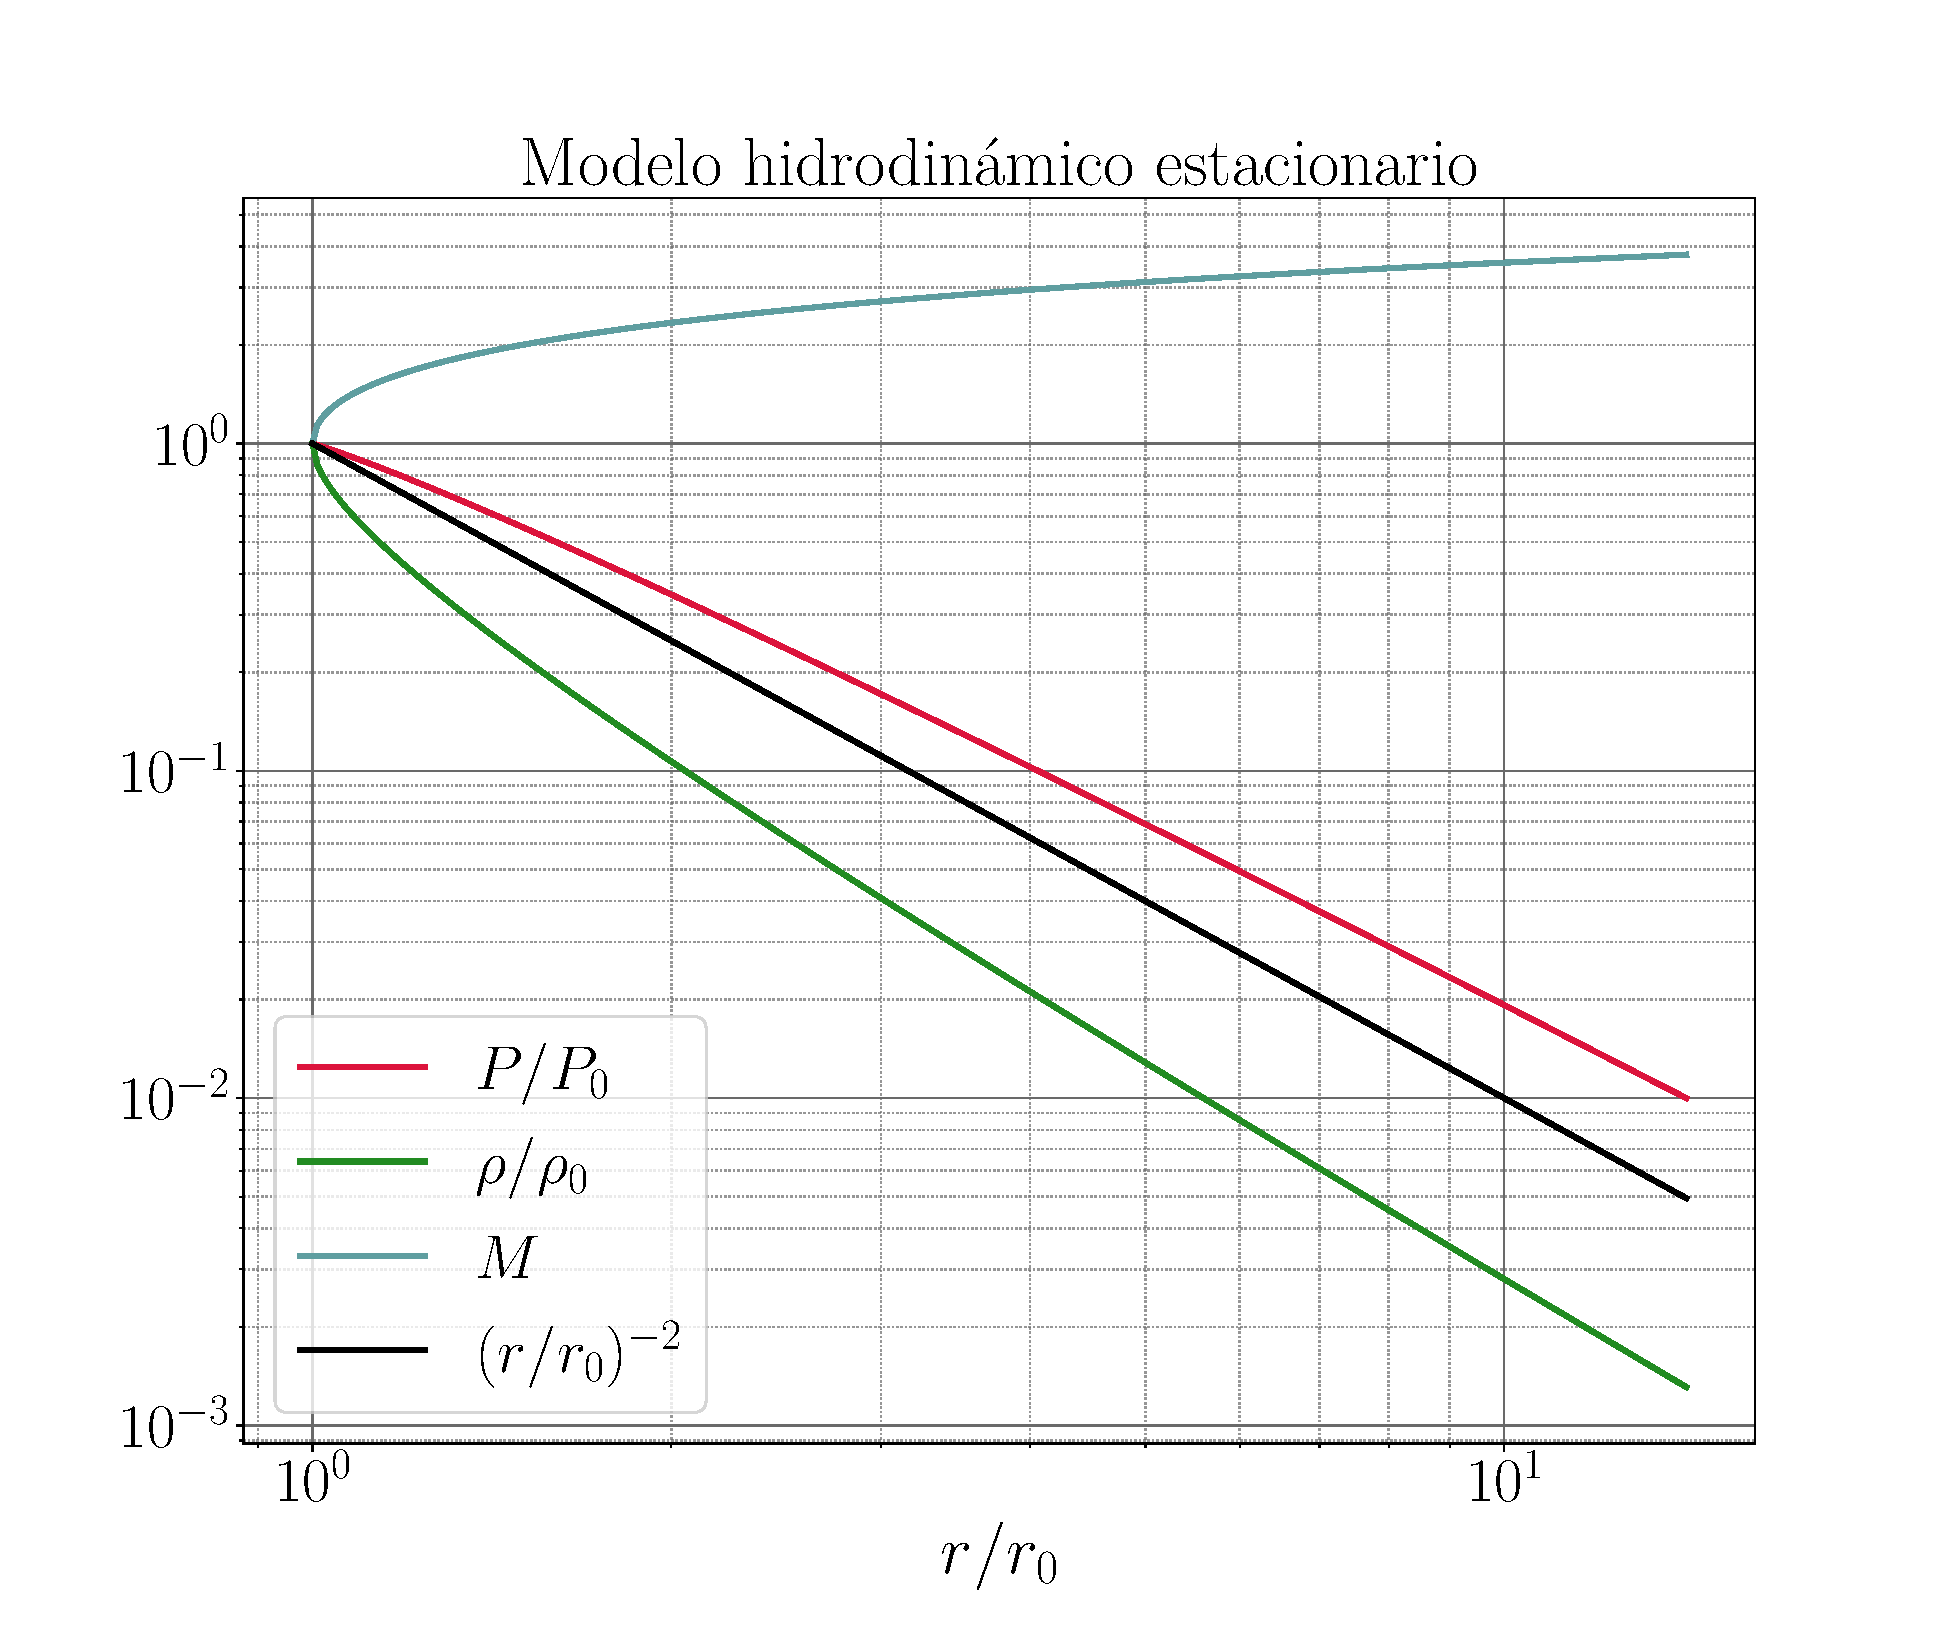
\includegraphics[width=\textwidth]{Nuevas imagenes finales/C2_estructura.pdf}
    \caption{Normalized Mach number $M$, density $\rho$, and total
      pressure $P$ as functions of $r/r_0$. A reference decline
      $\sim r^{-2}$ is also shown (black line). Note that the density
      falls more steeply than $r^{-2}$, while the total pressure
      declines more slowly; in both cases this is due to the
      acceleration of the flow.}
    \label{fig:grafica_C2}
  \end{figure}
  
% \section{Condiciones para la cáscara chocada}

% \cite{Canto:1996} en su descripción para interacción de dos flujos
% hipersónicos da la solución a distintos parámetros
% $\beta=(\dot{M}^0_\mathrm{w}
% v_\mathrm{w})/(\dot{M}^0_\mathrm{w1}v_\mathrm{w1})$, el cual es la
% razón de los momentos de los flujos $\mathrm{w}$ y $\mathrm{w1}$. Esto
% se puede ver en la Figura \ref{fig:Canto2} en la cual notamos que
% cuando el momento de un flujo es muy grande comparado con el otro, la
% cáscara chocada se vuelve muy curva y está más cerca de la fuente cuyo
% flujo tiene menor momento.

% \begin{figure}[htb]
%     \centering    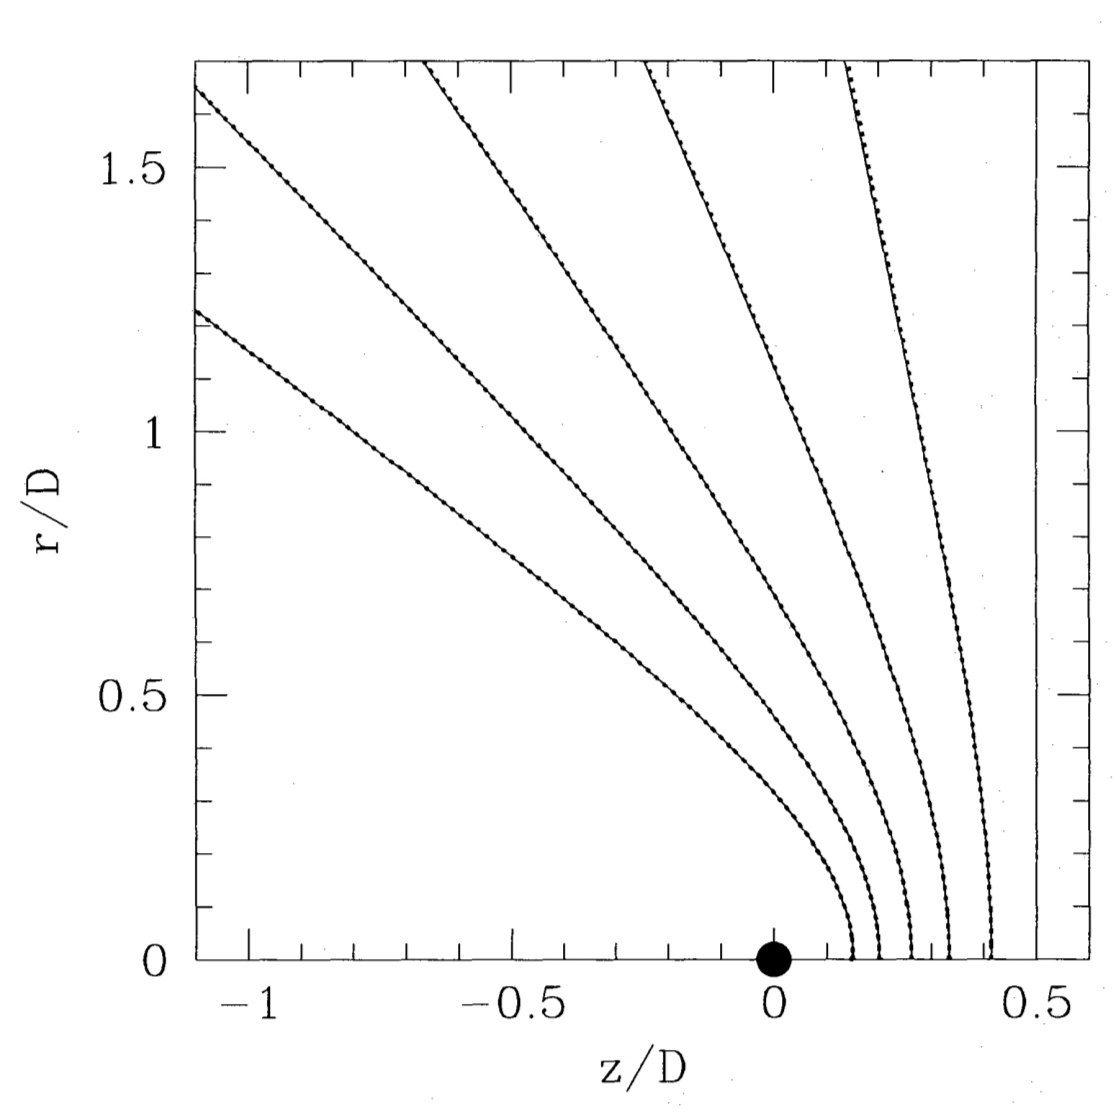
\includegraphics[width=0.8\textwidth]{images Chapter 2/C2_Canto2.jpg}
%     \caption{Formas de las distintas cáscaras chocadas a diferentes
%       parámetros $\beta$. La línea vertical en z/D=0.5 corresponde a un
%       parámetro $\beta=1$ y las demás curvas corresponden a valores de
%       0.5, 0.25, 0.125, 0.0625 y 0.03125, entre más pequeño es $\beta$ más
%       curva se vuelve la cáscara chocada. La otra fuente se encuentra
%       en z/D=1 \citep{Canto:1996}.}
%     \label{fig:Canto2}
% \end{figure}

% En la Figura \ref{fig:zones_presiones} vemos los diferentes tipos de
% presiones que hay en cada zona en esta interacción entre flujos
% supersónicos. En la zona de discontinuidad, la línea gris en la Figura
% \ref{fig:zones_presiones}, será la suma de la presión RAM del viento
% estelar, $P_\mathrm{RAM}$, y de la presión térmica del viento estelar.
% Dado que los vientos estelares en estrellas Wolf-Rayet llegan a ser
% del orden de \SI{1e3}{km.s^{-1}} podríamos llegar a tener un número de
% Mach del orden de 100 para el viento estelar, por lo que vamos a
% considerar que $P_\mathrm{DC}=P_\mathrm{RAM}$. Por otro lado, para la
% cáscara chocada, la zona 2 de la Figura \ref{fig:zones}, tenemos que
% esta debe estar en doble equilibrio de presión. Por un lado, la
% presión de la cáscara chocada, $P_\mathrm{shell}$ debe ser igual a la
% presión del flujo fotoevaporativo justo antes del choque, es decir,
% $P_\mathrm{shell}=P$. Por el otro lado, la presión de la cáscara
% chocada debe ser igual a la presión RAM del viento estelar chocado.

% \begin{figure}[htb]
%     \centering    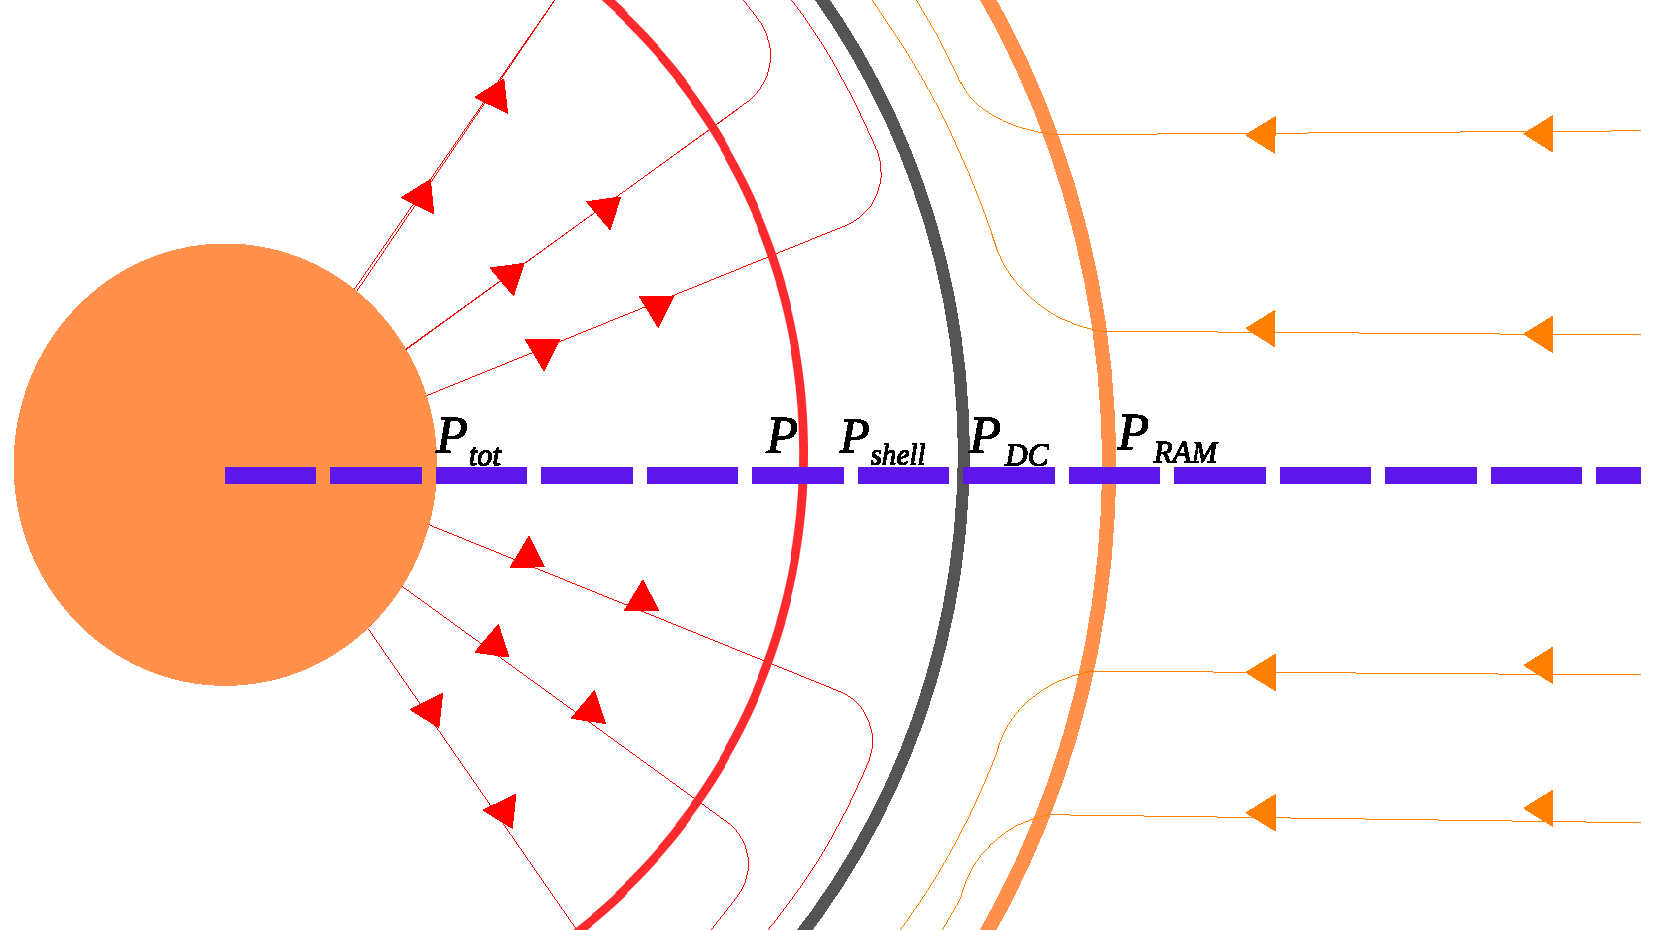
\includegraphics[width=\textwidth]{imagenes_corregidas/Arreglo 03.pdf}
%     \caption{La base del glóbulo está dominada por la presión total,
%       ecuación (\ref{eq: Presion total}). En la línea roja, que es la
%       parte más interna de la cáscara chocada, tenemos que domina la
%       presión térmica del flujo fotoevaporativo $P$. En la línea
%       naranja domina la presión RAM del viento estelar
%       $P_\mathrm{RAM}$, la cual es la única presión externa que
%       estamos considerando. En la zona de discontinuidad tenemos una
%       presión $P_\mathrm{DC}$, la cual es la suma de la presión RAM
%       del viento estelar y la presión térmica del viento estelar
%       chocado. }
%     \label{fig:zones_presiones}
% \end{figure}

\section{Conditions for the shocked shell}

In their description of the interaction between two hypersonic flows,
\cite{Canto:1996} derive solutions for different parameters
$\beta=(\dot{M}^0_\mathrm{w}
v_\mathrm{w})/(\dot{M}^0_\mathrm{w1}v_\mathrm{w1})$, which is the
ratio of the momentum fluxes of flows $\mathrm{w}$ and $\mathrm{w1}$.
This can be seen in Figure \ref{fig:Canto2}, where we note that when
the momentum of one flow is much greater than that of the other, the
shocked shell becomes highly curved and lies closer to the source with
the weaker momentum flux.

\begin{figure}[htb]
    \centering    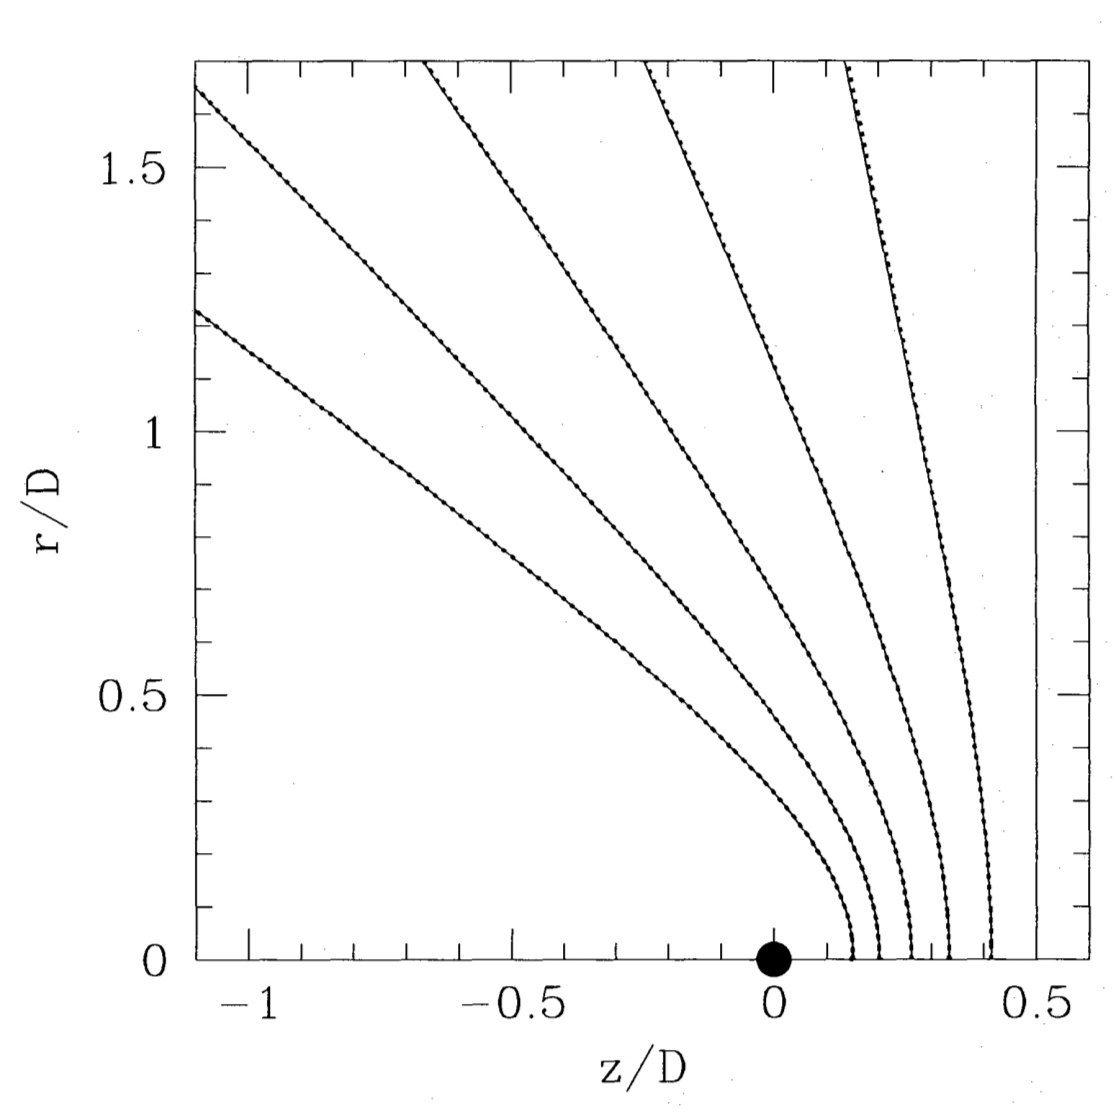
\includegraphics[width=0.8\textwidth]{images Chapter 2/C2_Canto2.jpg}
    \caption{Shapes of shocked shells for different values of the
      parameter $\beta$. The vertical line at $z/D=0.5$ corresponds to
      $\beta=1$, while the other curves correspond to 0.5, 0.25,
      0.125, 0.0625, and 0.03125. The smaller the $\beta$, the more
      curved the shocked shell becomes. The other source is located at
      $z/D=1$ \citep{Canto:1996}.}
    \label{fig:Canto2}
\end{figure}

Figure \ref{fig:zones_presiones} shows the different types of
pressures in each zone of this interaction between supersonic flows.
At the discontinuity (the gray line in Figure
\ref{fig:zones_presiones}), the pressure is the sum of the stellar
wind RAM pressure, $P_\mathrm{RAM}$, and the thermal pressure of the
stellar wind. Since the stellar winds of Wolf--Rayet stars can reach
velocities of order \SI{1e3}{km.s^{-1}}, the Mach number of the
stellar wind can be of order 100, so we will assume that
$P_\mathrm{DC}=P_\mathrm{RAM}$. On the other hand, for the shocked
shell (zone 2 of Figure \ref{fig:zones}), double pressure equilibrium
must hold. First, the pressure in the shocked shell,
$P_\mathrm{shell}$, must equal the pressure of the photoevaporative
flow immediately upstream of the shock, i.e.,
$P_\mathrm{shell}=P$. Second, the pressure in the shocked shell must
equal the RAM pressure of the shocked stellar wind.

\begin{figure}[htb]
    \centering    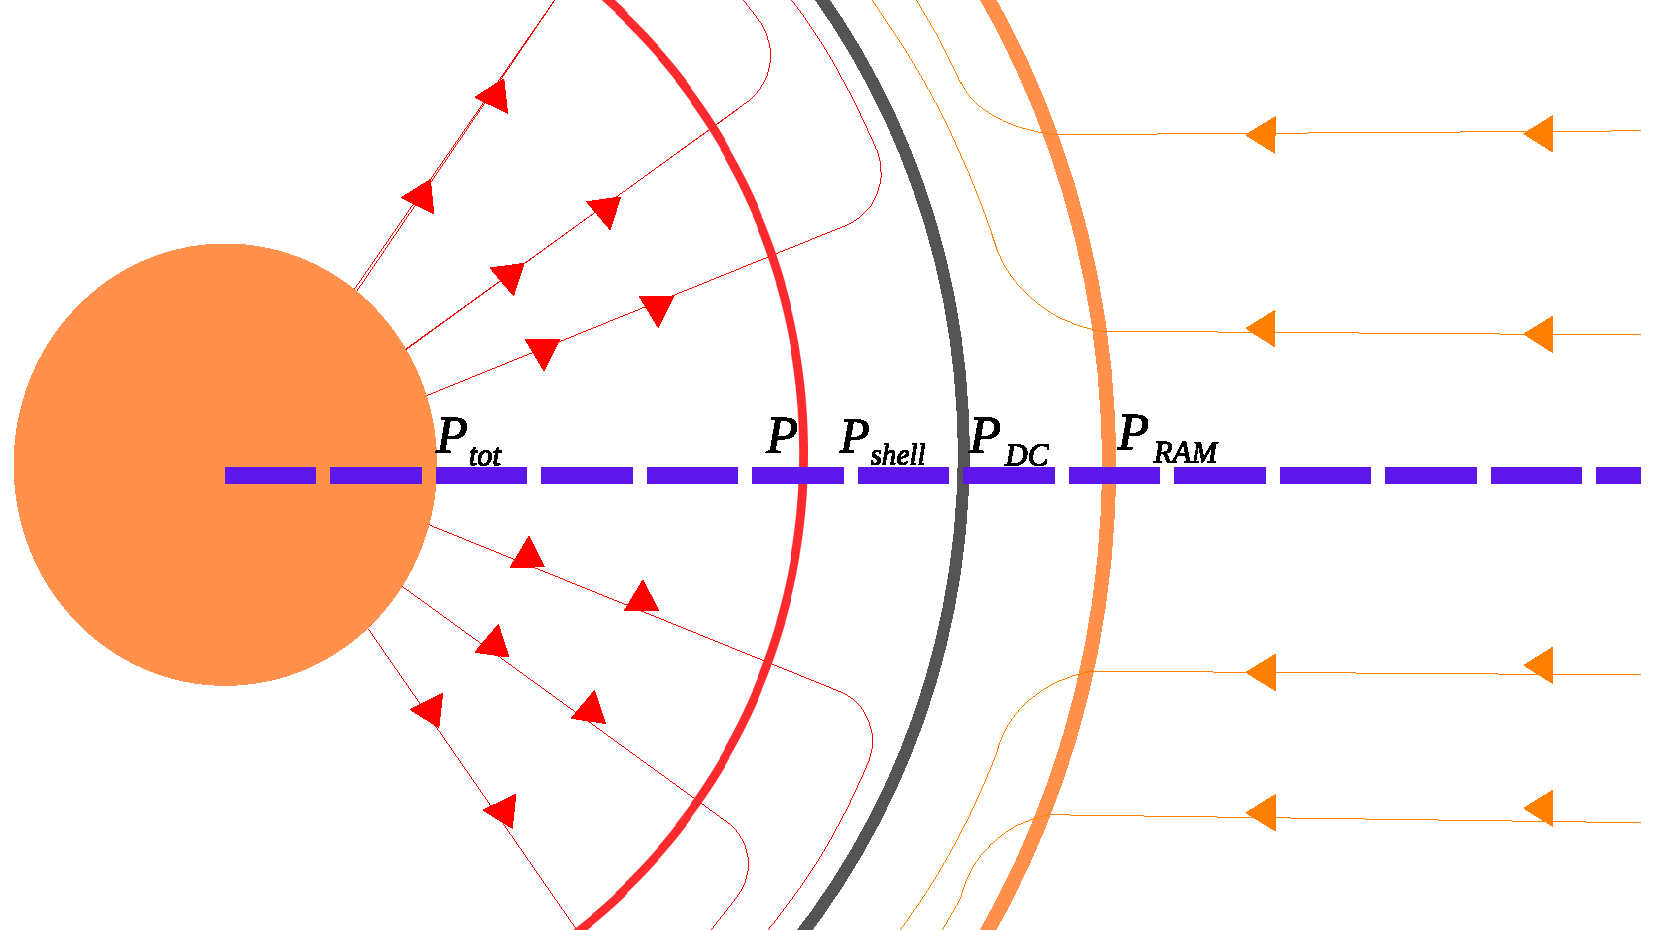
\includegraphics[width=\textwidth]{imagenes_corregidas/Arreglo 03.pdf}
    \caption{The base of the globule is dominated by the total
      pressure, equation (\ref{eq: Presion total}). Along the red
      line, which is the innermost part of the shocked shell, the
      pressure is dominated by the thermal pressure of the
      photoevaporative flow, $P$. Along the orange line the pressure
      is dominated by the RAM pressure of the stellar wind,
      $P_\mathrm{RAM}$, which is the only external pressure we are
      considering. At the discontinuity there is a pressure
      $P_\mathrm{DC}$, which is the sum of the stellar wind RAM
      pressure and the thermal pressure of the shocked stellar wind.}
    \label{fig:zones_presiones}
\end{figure}





% \chapter{Glóbulos en la nebulosa M1-67} \label{Chapter : 3}

% Ahora vamos a describir cómo encontramos estos glóbulos en la nebulosa
% M1-67. En la Figura \ref{fig:nudos WR124} vemos del lado derecho cómo
% estos glóbulos los podemos identificar de manera visual por tres
% componentes importantes. El glóbulo lo vemos como un círculo de color
% blanco, su estela de color rosa que se encuentra justo detrás del
% glóbulo en dirección opuesta a la estrella, y su cáscara chocada que
% se ve de color gris. De esta manera, se pudieron localizar visualmente
% 168 glóbulos en total.

% De las observaciones vemos que estos glóbulos tienen tamaños típicos
% de 200--300 mili segundos de arco (5--\SI{7e-3}{pc}) de diámetro que son
% relativamente pequeños si los comparamos con la nebulosa circunestelar
% que es de unos $\sim\SI{60}{\arcsecond}$ (\SI{1.57}{pc}).

% \begin{figure}[htb]
%     \centering
%     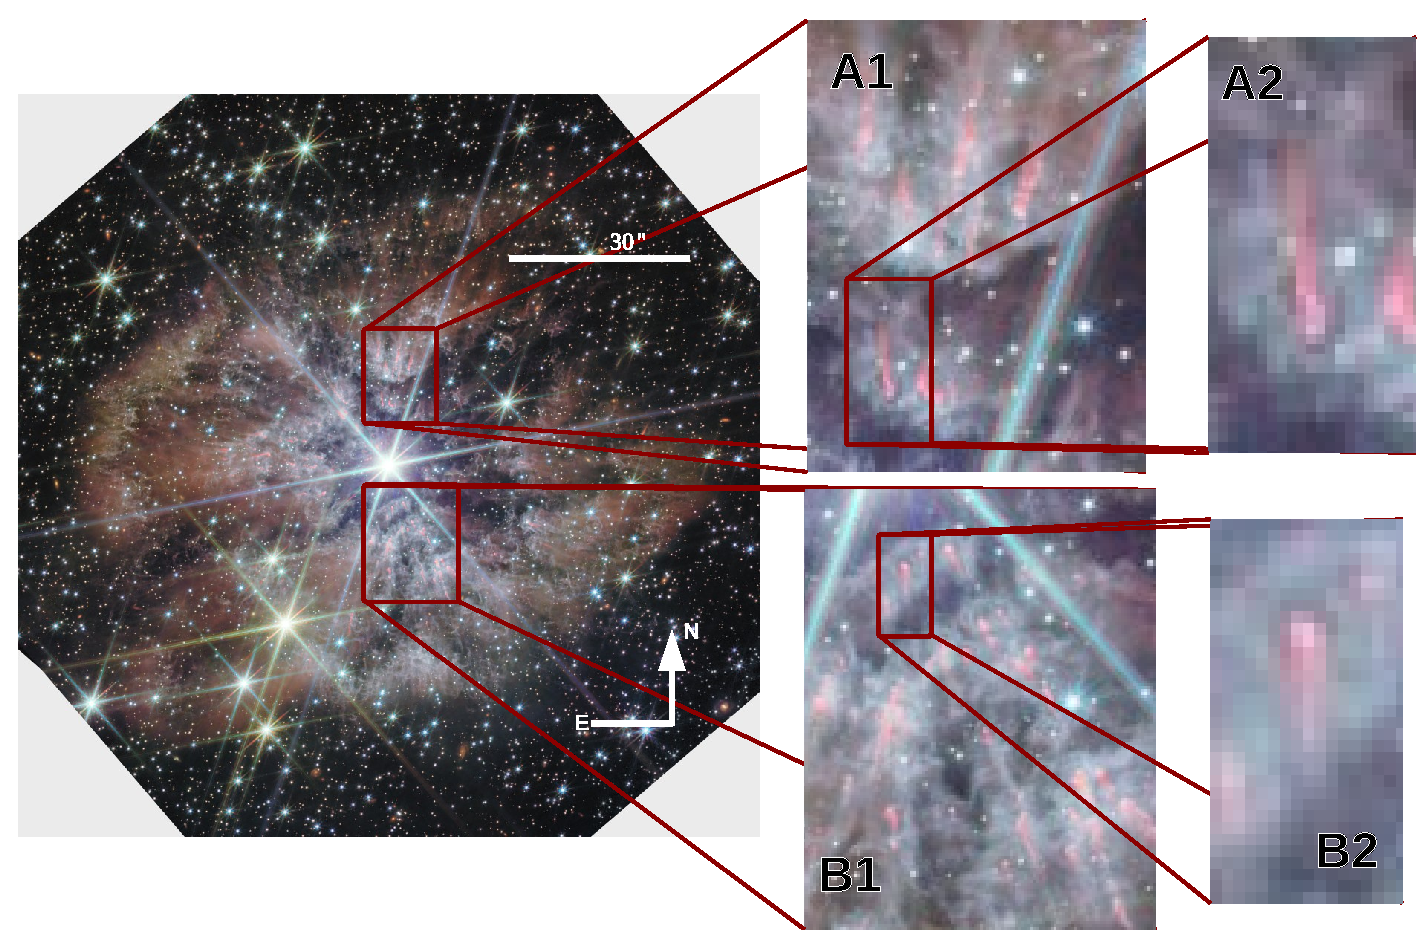
\includegraphics[width=\textwidth]{ultimas correcciones/WR124_glo_ej.pdf}
%     \caption{En esta imagen capturada con el JWST vemos la nebulosa
%       M1-67 y en ella la presencia de glóbulos en casi toda la
%       nebulosa. Haciendo zoom en estos glóbulos (la emisión en color
%       blanco y rosa), vemos como puede ser su morfología en la parte
%       neutra debido a la emisión de PAHs. Mientras que en color gris
%       vemos lo que parece ser su interacción con la estrella y su
%       viento estelar. Las figuras A1, A2, B1 y B2 tienen medidas de
%       $\SI{11.86}{\arcsecond}\times\SI{15.65}{\arcsecond}$
%       ($\SI{0.31}{pc}\times\SI{.41}{pc}$),
%       $\SI{2.94}{\arcsecond}\times\SI{5.76}{\arcsecond}$
%       ($\SI{0.07}{pc}\times\SI{0.15}{pc}$),
%       $\SI{15.82}{\arcsecond}\times\SI{19.21}{\arcsecond}$
%       ($\SI{0.41}{pc}\times\SI{0.5}{pc}$) y
%       $\SI{2.42}{\arcsecond}\times\SI{4.53}{\arcsecond}$
%       ($\SI{0.06}{pc}\times\SI{0.11}{pc}$), respectivamente.}
%     \label{fig:nudos WR124}
% \end{figure}

% A estos glóbulos los podemos localizar por su posición angular y
% separación con respecto a la estrella. La posición angular es el
% ángulo $\phi$ que tiene con respecto a la línea roja de la Figura
% \ref{fig:ejemplo_PA_Sep}, esta línea roja representa la posición
% angular a $0^\circ$, y el ángulo $\phi$ es tomado en sentido contrario a las
% manecillas del reloj. La separación entre el glóbulo y la estrella es
% medido directamente de las observaciones. En la Figura
% \ref{fig:ejemplo_PA_Sep} vemos un ejemplo de como podemos conocer la
% posición angular y separación para cada glóbulo.

% \begin{figure}[htb]
%     \centering
%     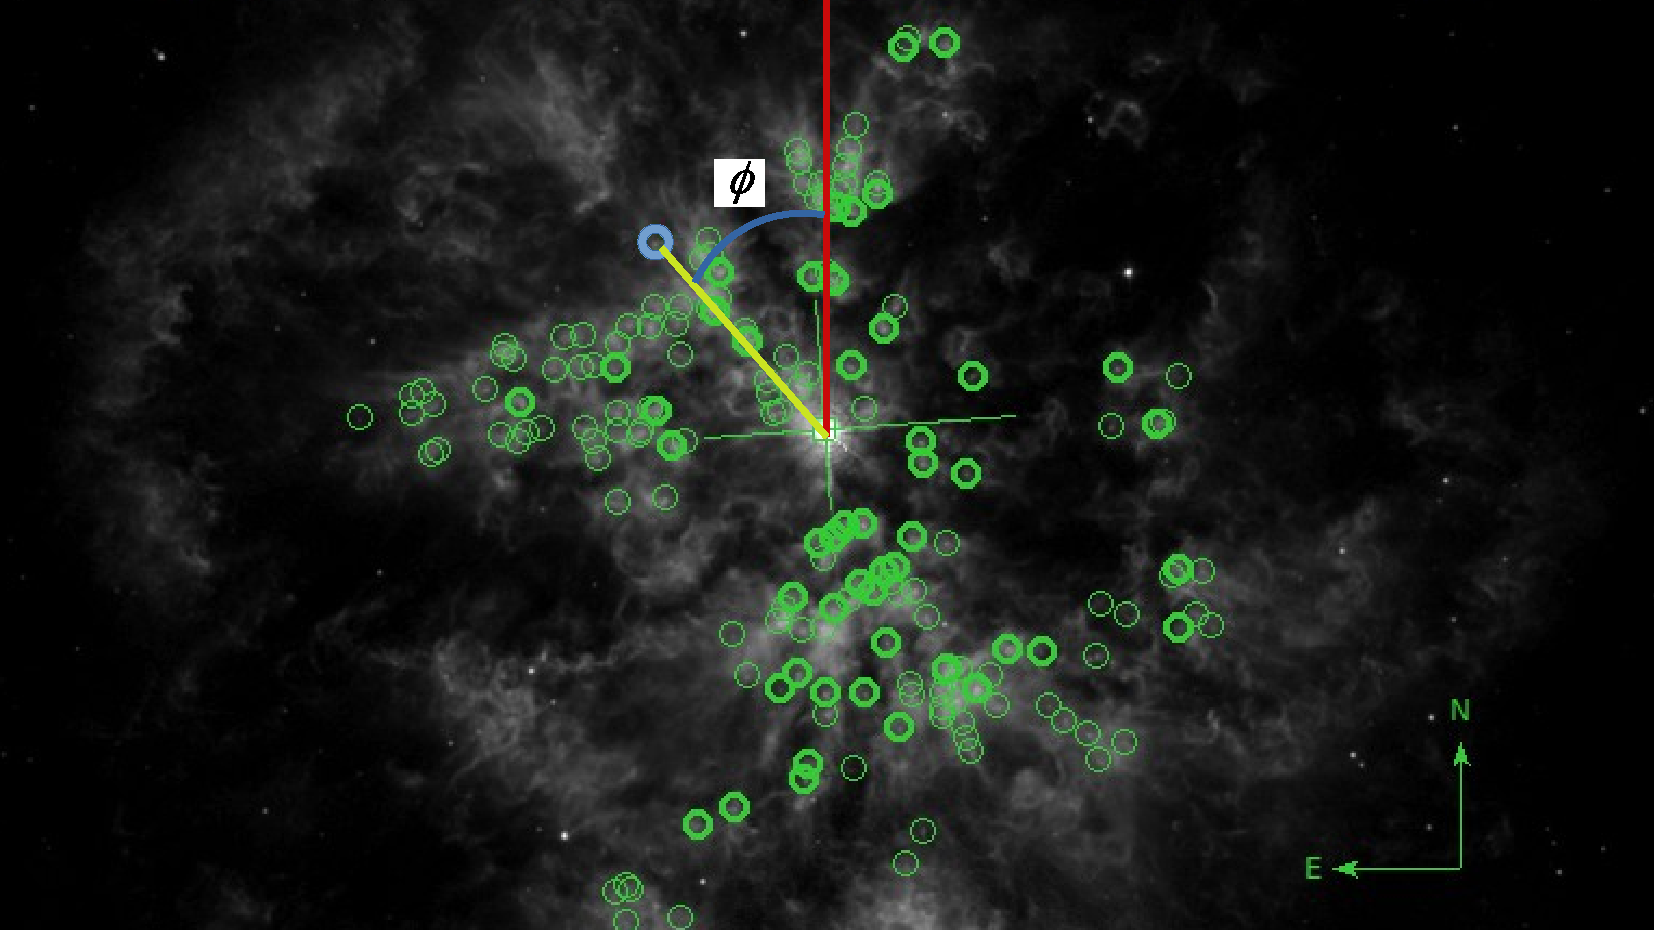
\includegraphics[width=\textwidth]{ultimas correcciones/M167_PA.pdf}
%     \caption{En esta imagen vemos un ejemplo de como obtuvimos la
%       posición angular y la separación con respecto a la estrella. El
%       círculo azul es el glóbulo que tomaremos como ejemplo, el ángulo
%       $\phi$ con respecto a la línea roja es la posición angular y es
%       tomada en sentido anti horario, la separación es la longitud de
%       la línea amarilla, la cual une al glóbulo (círculo azul) con la
%       estrella, la cual se encuentra en el centro de la imagen. Los
%       puntos verdes marcan donde se localizan los otros glóbulos.}
%     \label{fig:ejemplo_PA_Sep}
% \end{figure}

% En la Figura \ref{fig:dis_nudos} vemos del lado izquierdo la
% localización de los glóbulos en la nebulosa, donde los puntos verdes
% son los glóbulos que encontramos y la línea roja es nuestra referencia
% para encontrar su posición angular. En el lado derecho vemos como
% estos se distribuyen considerando su separación y posición angular. En
% estas distribuciones podemos encontrar ciertas simetrías, por ejemplo,
% en el histograma superior de la imagen izquierda vemos que muchos de
% estos glóbulos se concentran en dos posiciones angulares en
% particular, a $\sim90^\circ$ y $\sim200^\circ$, mientras que a
% $120^\circ$ y $300^\circ$ no tenemos casi glóbulos. Por otro lado, en el
% histograma del lado derecho vemos cómo en separación pareciera haber
% una distribución bimodal con picos a \SI{11}{\arcsecond}
% (\SI{.28}{pc)} y \SI{17}{\arcsecond} (\SI{.44}{pc}). Esta distribución
% nos dice que la cantidad de glóbulos decae con la distancia de manera
% no constante, mientras que los grupos de glóbulos encontrados parecen
% ser los causantes de los picos de la distribución.

% \begin{figure}[htb]
%     \centering  
%     \begin{subfigure}[b]{0.45\linewidth}
%         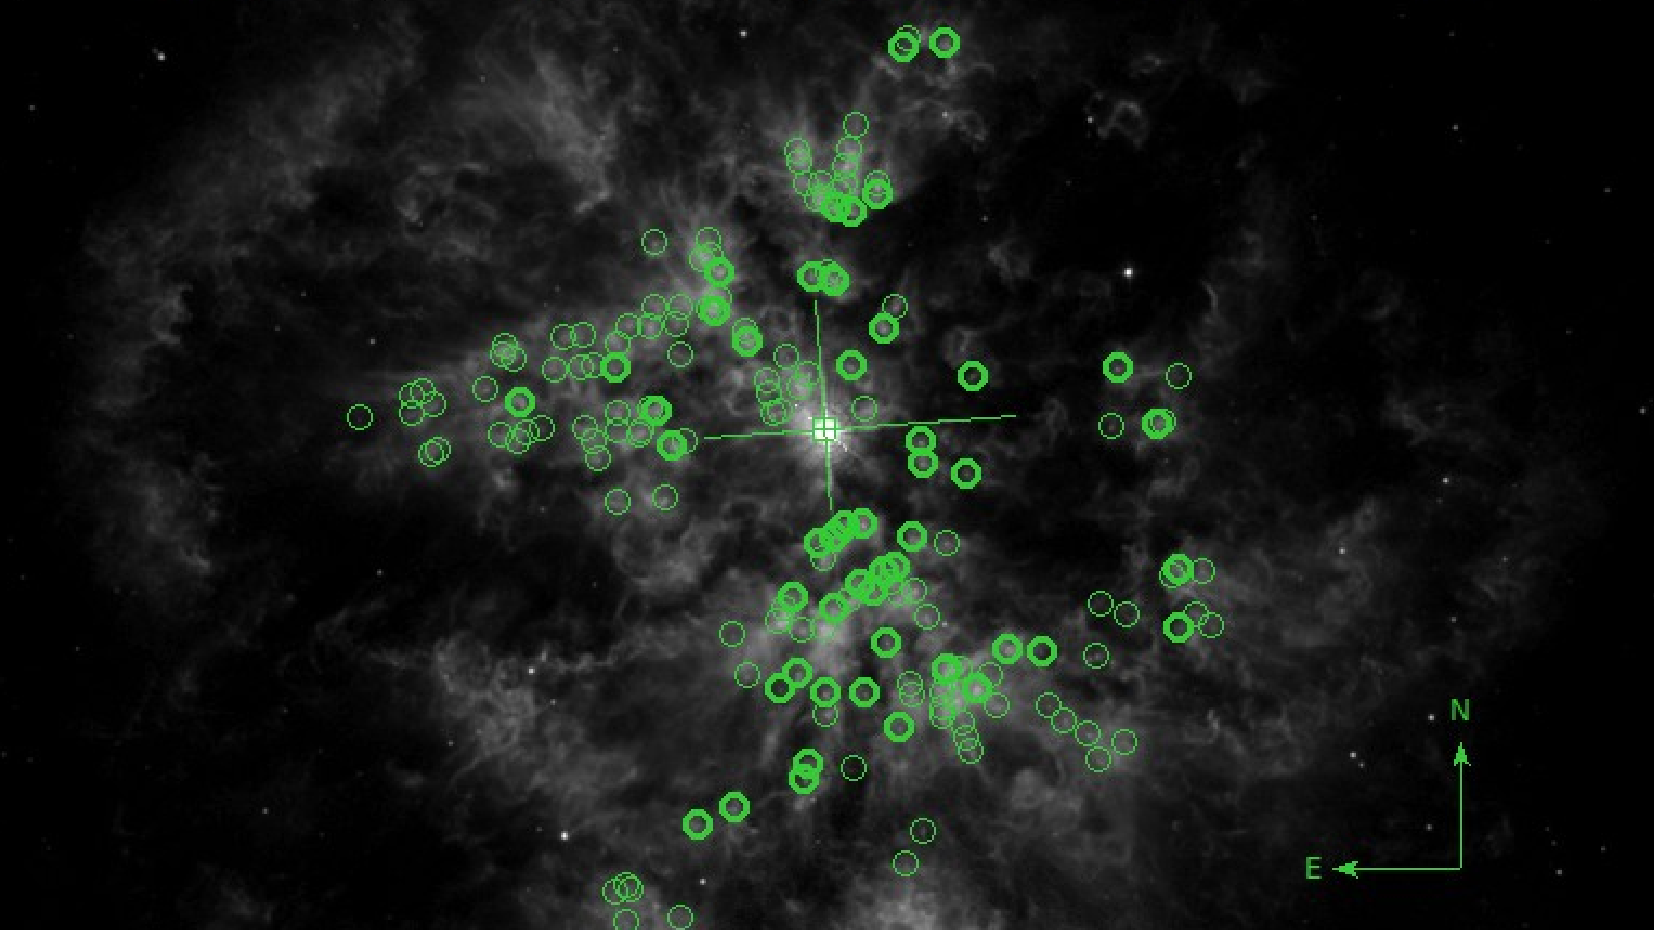
\includegraphics[width=\textwidth]{ultimas correcciones/M167_glo.pdf}
%     \end{subfigure}
%     \begin{subfigure}[b]{0.45\linewidth}
%         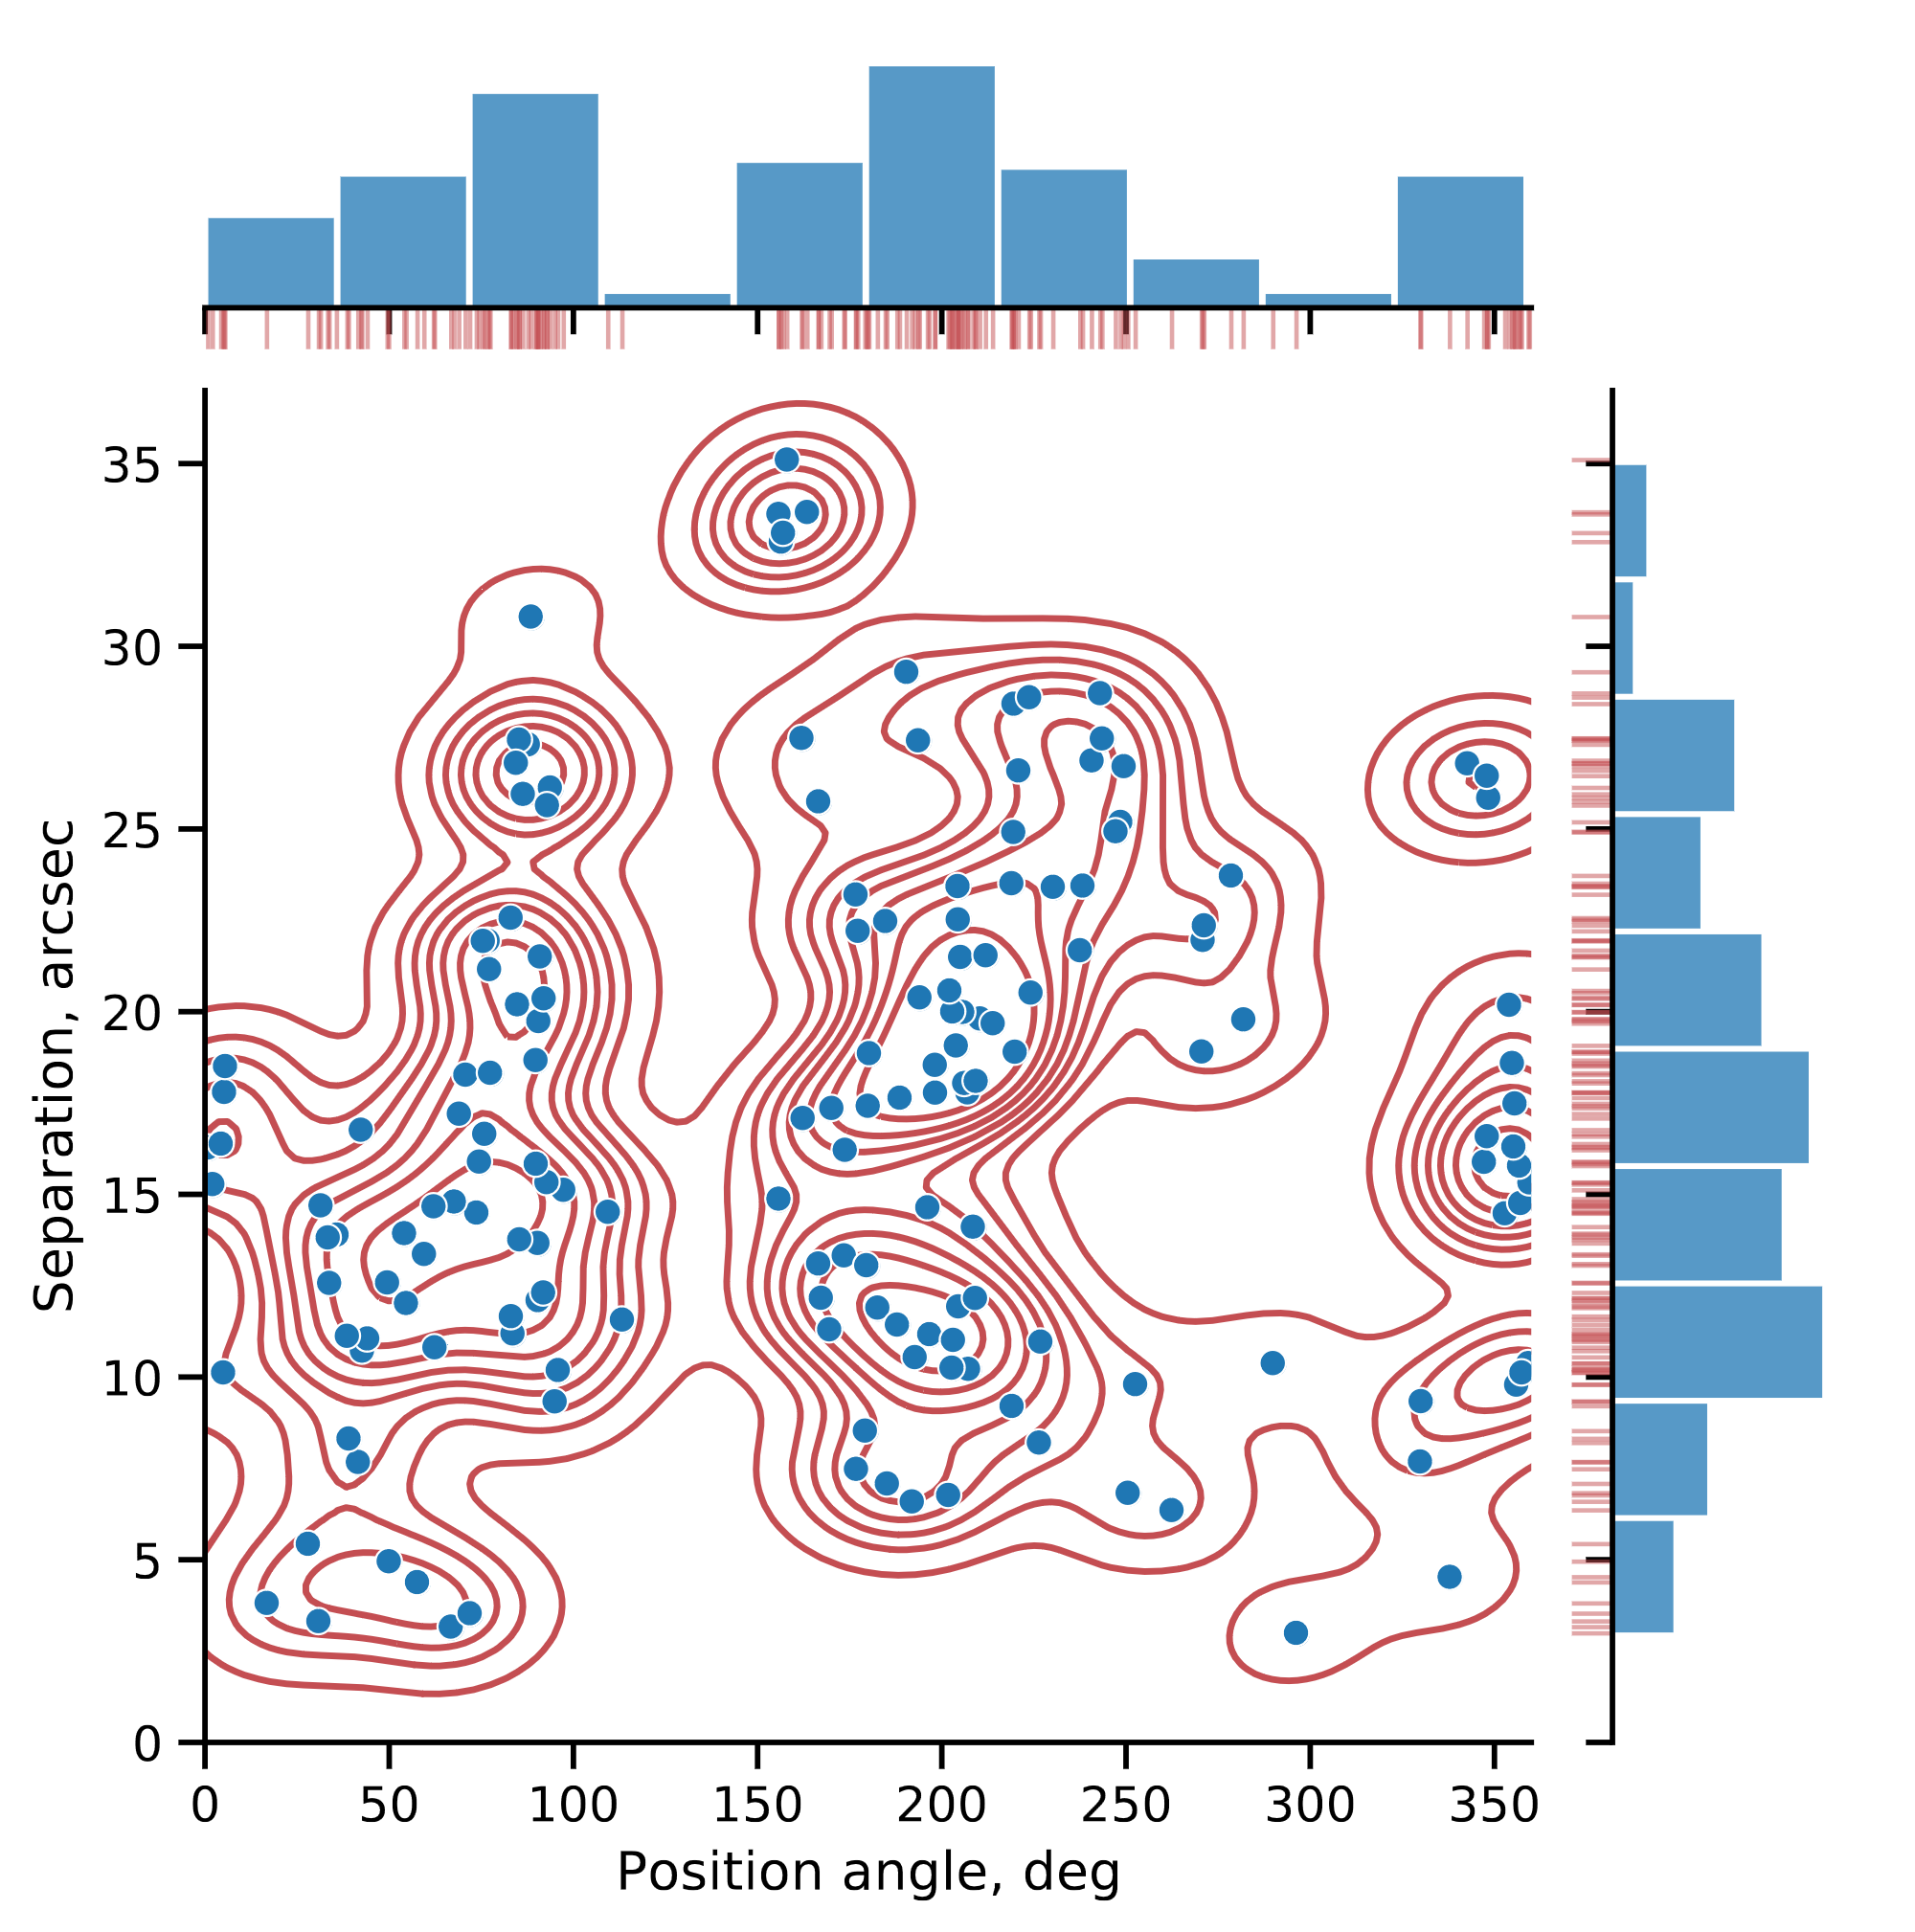
\includegraphics[width=\textwidth]{images Chapter 2/C2_nudos_distribucion.png}
%     \end{subfigure}
%     \caption{En la imagen izquierda vemos en puntos verde la
%       localización de los glóbulos en la nebulosa M1-67 y la línea
%       roja es la que usamos para conocer la posición angular de cada
%       glóbulo. En la imagen derecha vemos como es la distribución de
%       estos glóbulos (puntos azules) en separación y posición angular.
%       En la parte superior de la imagen derecha vemos el histograma de
%       la posición angular y del lado derecho el histograma de la
%       separación de los glóbulos. Las líneas rojas son los
%       isocontornos de la densidad suavizada de la distribución de los
%       puntos.}
%     \label{fig:dis_nudos}
% \end{figure}

% En la Figura \ref{fig:filters WR124} vemos una gran variedad de
% glóbulos en una zona pequeña y sus diferentes morfologías que
% presentan en los diferentes filtros.

% Como ya hemos mencionado anteriormente, la interacción entre el flujo
% fotoevaporativo de los glóbulos y el viento estelar nos produce una
% cáscara chocada, la cual podemos ver debido a las recombinaciones, por
% lo que la podemos ver como emisión en algunos filtros. Por ejemplo, en
% el filtro f656n del HST y en los filtros f090w y f444w del JWST
% podemos ver esta cáscara chocada que rodea los glóbulos. También se
% realizó una combinación de filtros para poder ver solo la emisión de
% gas ionizado (ver Apéndice \ref{AP: combos}). Por lo que en la imagen
% de gas ionizado tenemos una imagen más clara del gas ionizado que se
% encuentra en la cáscara chocada.

% En el filtro f1130w del JWST se puede observar lo que parecen ser
% parte de las estelas de los glóbulos. Algunos parecen ser más pequeños
% que otros. También se pude notar que en algunos casos cuando los
% glóbulos están muy cerca los unos de los otros sus estelas parecen
% juntarse, incluso en algunos casos pareciera que estas estelas están
% interaccionando con otros glóbulos. En este filtro también se puede
% ver de manera muy tenue lo que pareciera ser la interacción del flujo
% fotoevaporativo por parte del gas y el viento estelar.

% También se hizo una combinación de filtros para poder ver solo la
% emisión de gas neutro (ver Apéndice \ref{AP: combos}. En este caso se
% puede observar mejor como es la morfología del glóbulo, por lo que
% aquí podemos conocer mejor sus propiedades.

% Con la gran variedad de imágenes que tenemos podemos hacer muchas
% comparaciones y ver los glóbulos en diferentes filtros y resoluciones,
% lo cual nos da muchas ventajas. Por ejemplo, las observaciones del
% JWST tienen mayor resolución, mientras que en el caso del filtro f656n
% del HST, debido a que es un filtro muy angosto, no se ve muy afectado
% por la emisión de las estrellas, a diferencia de las observaciones con
% el JWST.

% \begin{figure}[htb]
%     \centering
%     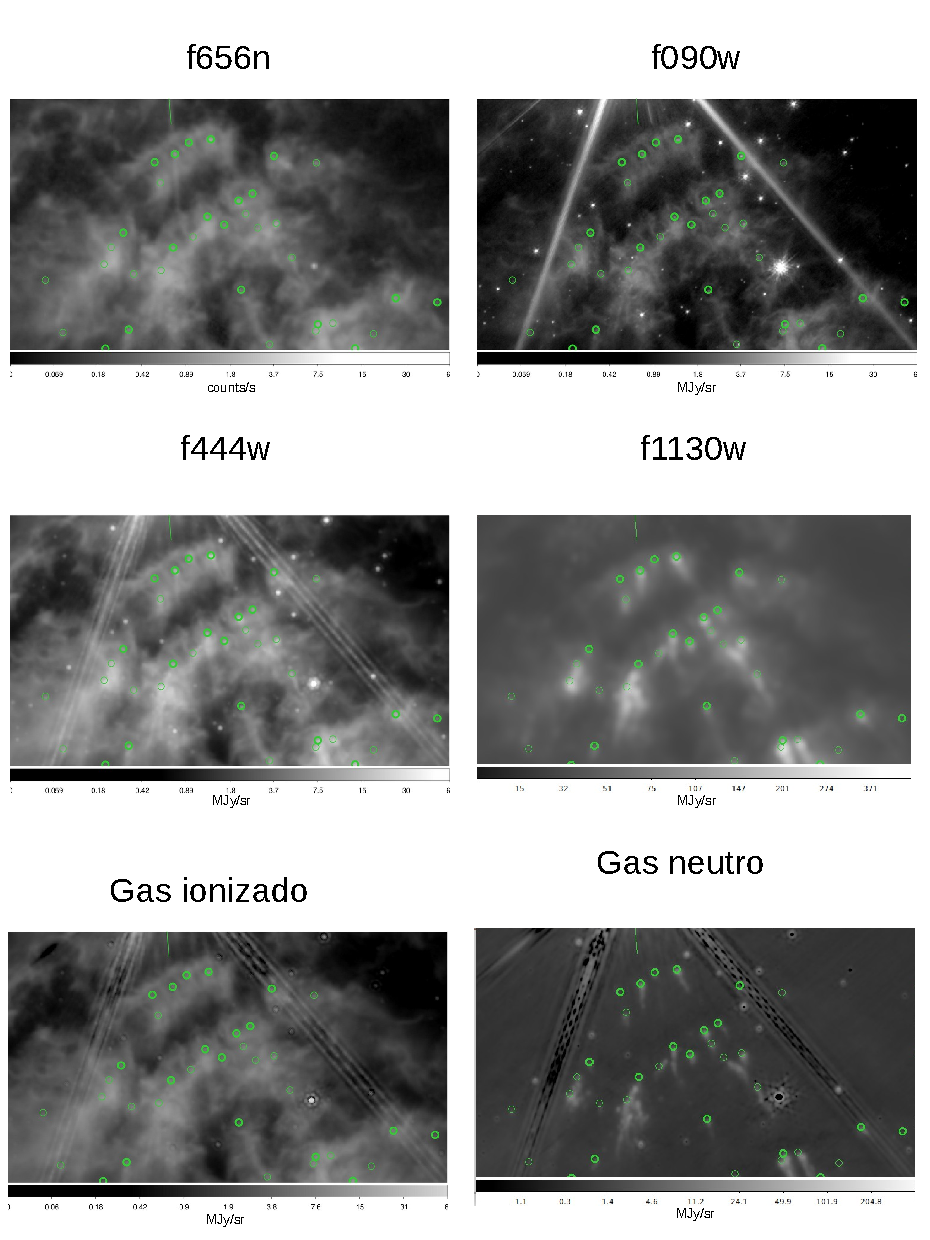
\includegraphics[width=\textwidth]{imagenes_corregidas/Arreglo_04.pdf}
%     \caption{La imagen del filtro f656n (esquina superior izquierda)
%       es la emisión de H$\alpha$ por parte del HST. Las demás imágenes son
%       utilizando los filtros del JWST. Para el caso del gas ionizado
%       se usó la siguiente combinación de filtros
%       f44w-0.43\,f335m-0.16(f150w-0.6\,f210m), mientras que para la
%       emisión de gas neutro se utilizó la combinación
%       1.4(f150w-0.6\;f210m)+f335m-0.95\;f210m. Los círculos verdes son
%       de los glóbulos.}
%     \label{fig:filters WR124}
% \end{figure}

\chapter{Globules in the M1-67 nebula} \label{Chapter : 3}

We now describe how we identified the globules in the M1-67 nebula. In
Figure \ref{fig:nudos WR124} (right panel) we see how these globules
can be visually recognized by three key components: the globule itself
appearing as a white circle; its pink tail, located immediately behind
the globule in the direction opposite to the star; and its shocked
shell, visible in gray. In this way we were able to identify a total
of 168 globules.

From the observations we see that these globules have typical sizes of
200--300 milliarcseconds (5--\SI{7e-3}{pc}) in diameter, which are
relatively small compared to the circumstellar nebula as a whole,
whose size is $\sim\SI{60}{\arcsecond}$ (\SI{1.57}{pc}).

\begin{figure}[htb]
    \centering
    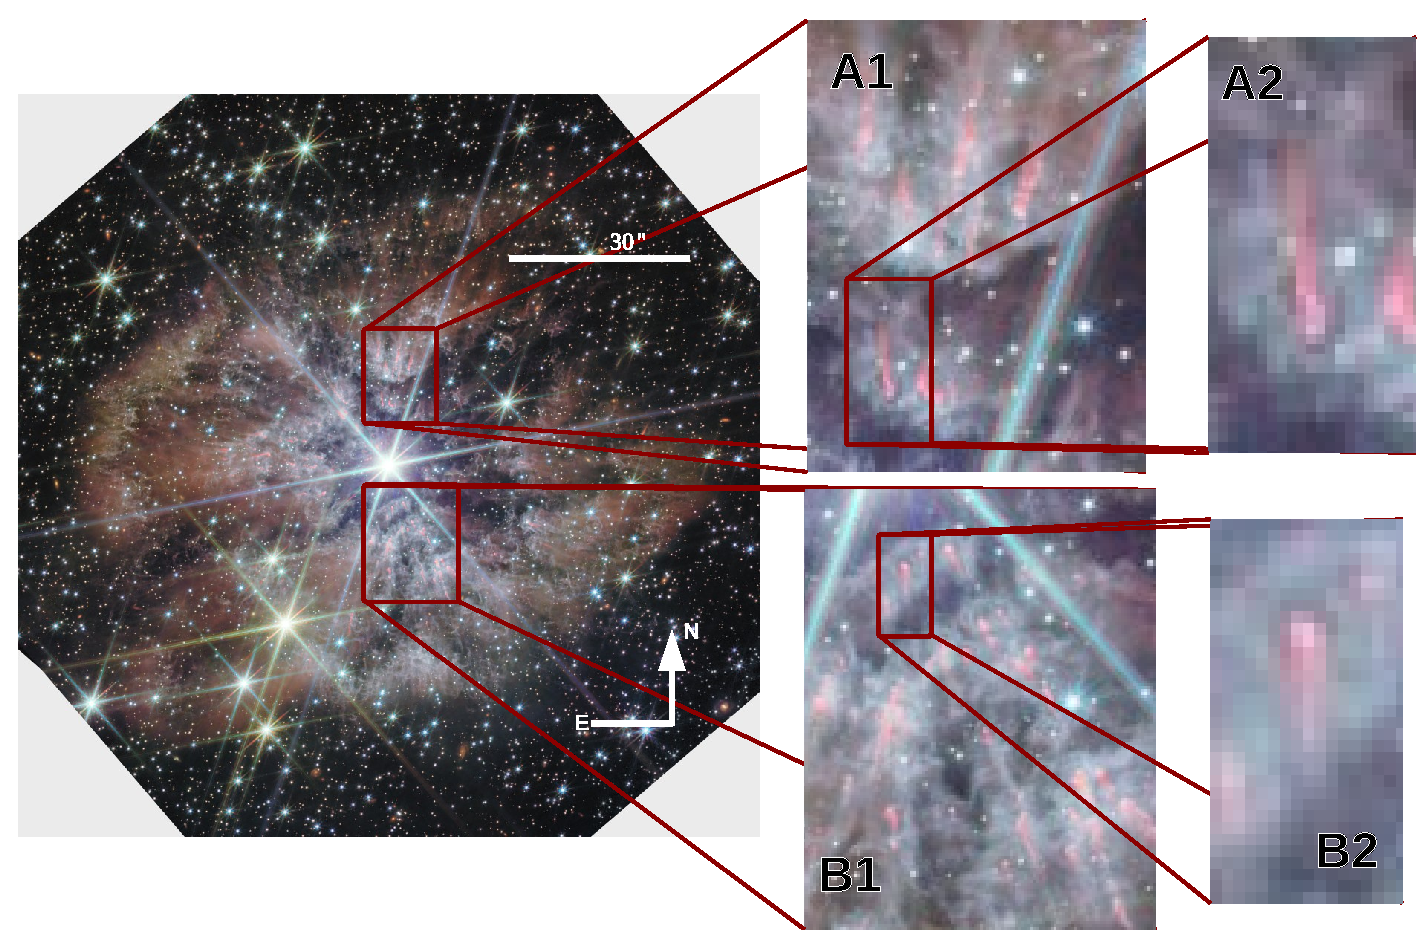
\includegraphics[width=\textwidth]{ultimas correcciones/WR124_glo_ej.pdf}
    \caption{Image of the M1-67 nebula captured with JWST showing
      globules throughout most of the nebula. Zooming in on individual
      globules (white and pink emission) reveals their morphology in
      the neutral component, traced by PAH emission, while the gray
      color indicates their interaction with the star and its stellar
      wind. Insets A1, A2, B1, and B2 have dimensions of
      $\SI{11.86}{\arcsecond}\times\SI{15.65}{\arcsecond}$
      ($\SI{0.31}{pc}\times\SI{.41}{pc}$),
      $\SI{2.94}{\arcsecond}\times\SI{5.76}{\arcsecond}$
      ($\SI{0.07}{pc}\times\SI{0.15}{pc}$),
      $\SI{15.82}{\arcsecond}\times\SI{19.21}{\arcsecond}$
      ($\SI{0.41}{pc}\times\SI{0.5}{pc}$), and
      $\SI{2.42}{\arcsecond}\times\SI{4.53}{\arcsecond}$
      ($\SI{0.06}{pc}\times\SI{0.11}{pc}$), respectively.}
    \label{fig:nudos WR124}
\end{figure}

The globules can be located by their angular position and separation
from the star. The angular position is the angle $\phi$ measured with
respect to the red line in Figure \ref{fig:ejemplo_PA_Sep}, which
defines the zero-degree reference. The angle $\phi$ is measured
counterclockwise. The separation between the globule and the star is
measured directly from the observations. Figure
\ref{fig:ejemplo_PA_Sep} shows an example of how we determine the
angular position and separation for each globule.

\begin{figure}[htb]
    \centering
    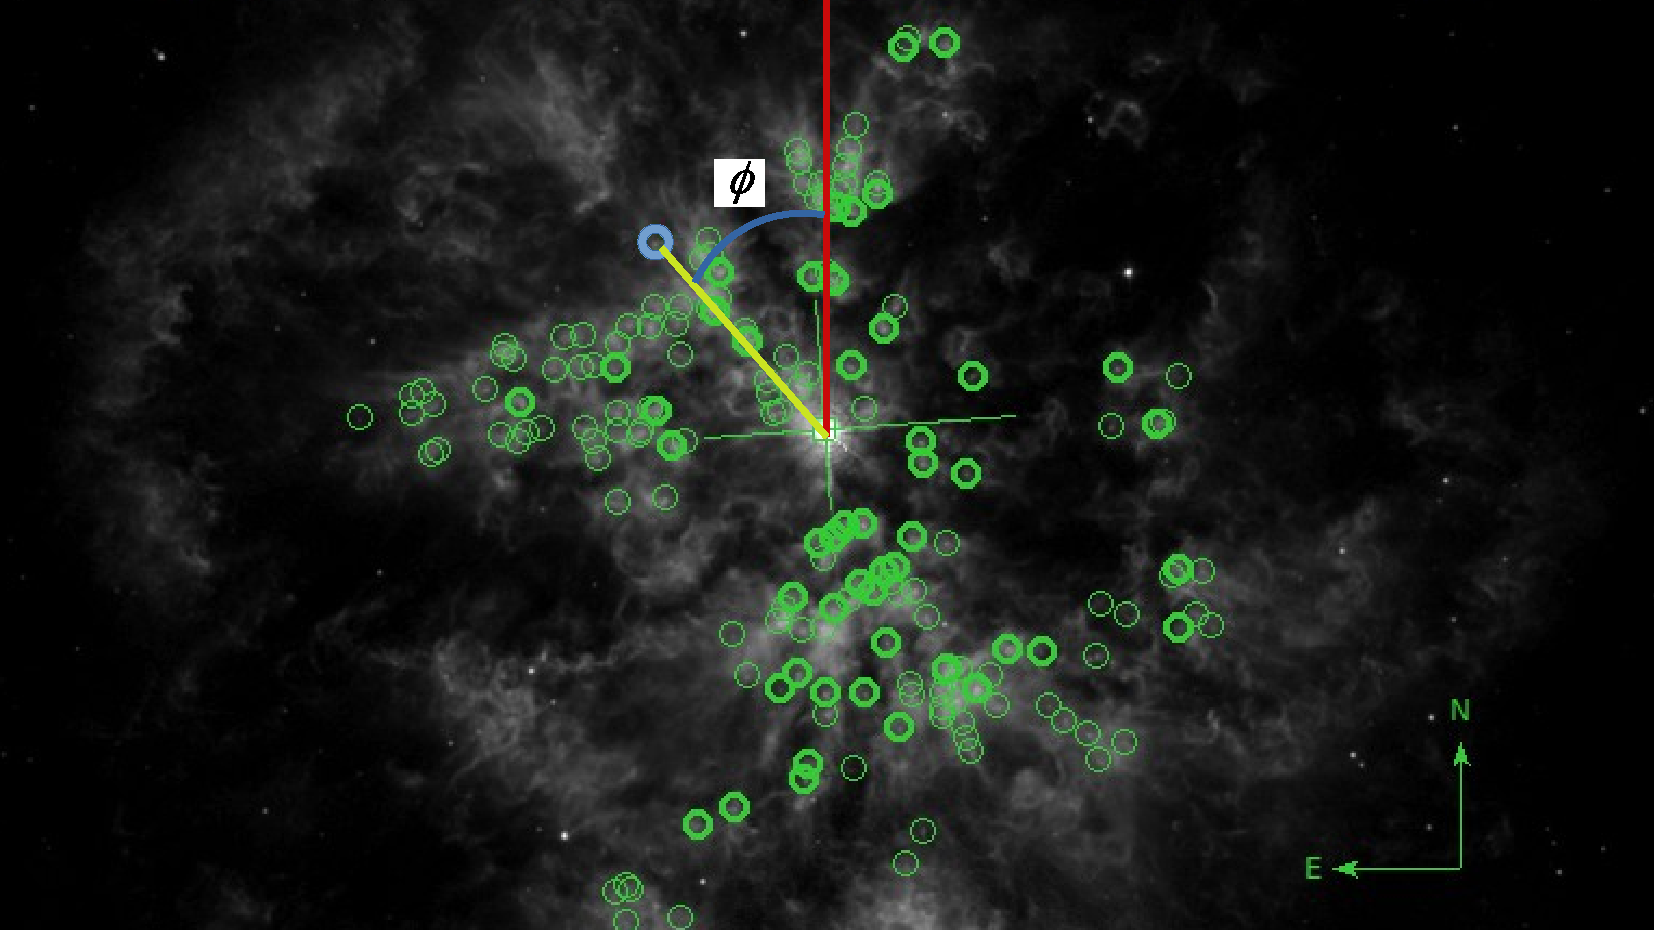
\includegraphics[width=\textwidth]{ultimas correcciones/M167_PA.pdf}
    \caption{Example of how we obtained the angular position and
      separation with respect to the star. The blue circle marks the
      globule used as an example; the angle $\phi$ with respect to the
      red line is the angular position, measured counterclockwise. The
      separation is the length of the yellow line connecting the
      globule (blue circle) with the star, located at the center of
      the image. The green points mark the positions of the other
      globules.}
    \label{fig:ejemplo_PA_Sep}
\end{figure}

In Figure \ref{fig:dis_nudos} (left) we see the spatial distribution
of the globules in the nebula: green points are the globules we
identified, and the red line is the reference used for angular
position. On the right we show their distribution as a function of
separation and angular position. Certain symmetries can be discerned.
For example, in the histogram at the top of the right-hand panel many
globules are concentrated at two particular angular positions,
$\sim90^\circ$ and $\sim200^\circ$, whereas at $120^\circ$ and
$300^\circ$ almost no globules are found. In the histogram on the
right we see an apparently bimodal distribution in separation, with
peaks at \SI{11}{\arcsecond} (\SI{.28}{pc}) and \SI{17}{\arcsecond}
(\SI{.44}{pc}). This distribution indicates that the number of
globules does not decline smoothly with distance, but instead that
groups of globules are responsible for the peaks in the distribution.

\begin{figure}[htb]
    \centering  
    \begin{subfigure}[b]{0.45\linewidth}
        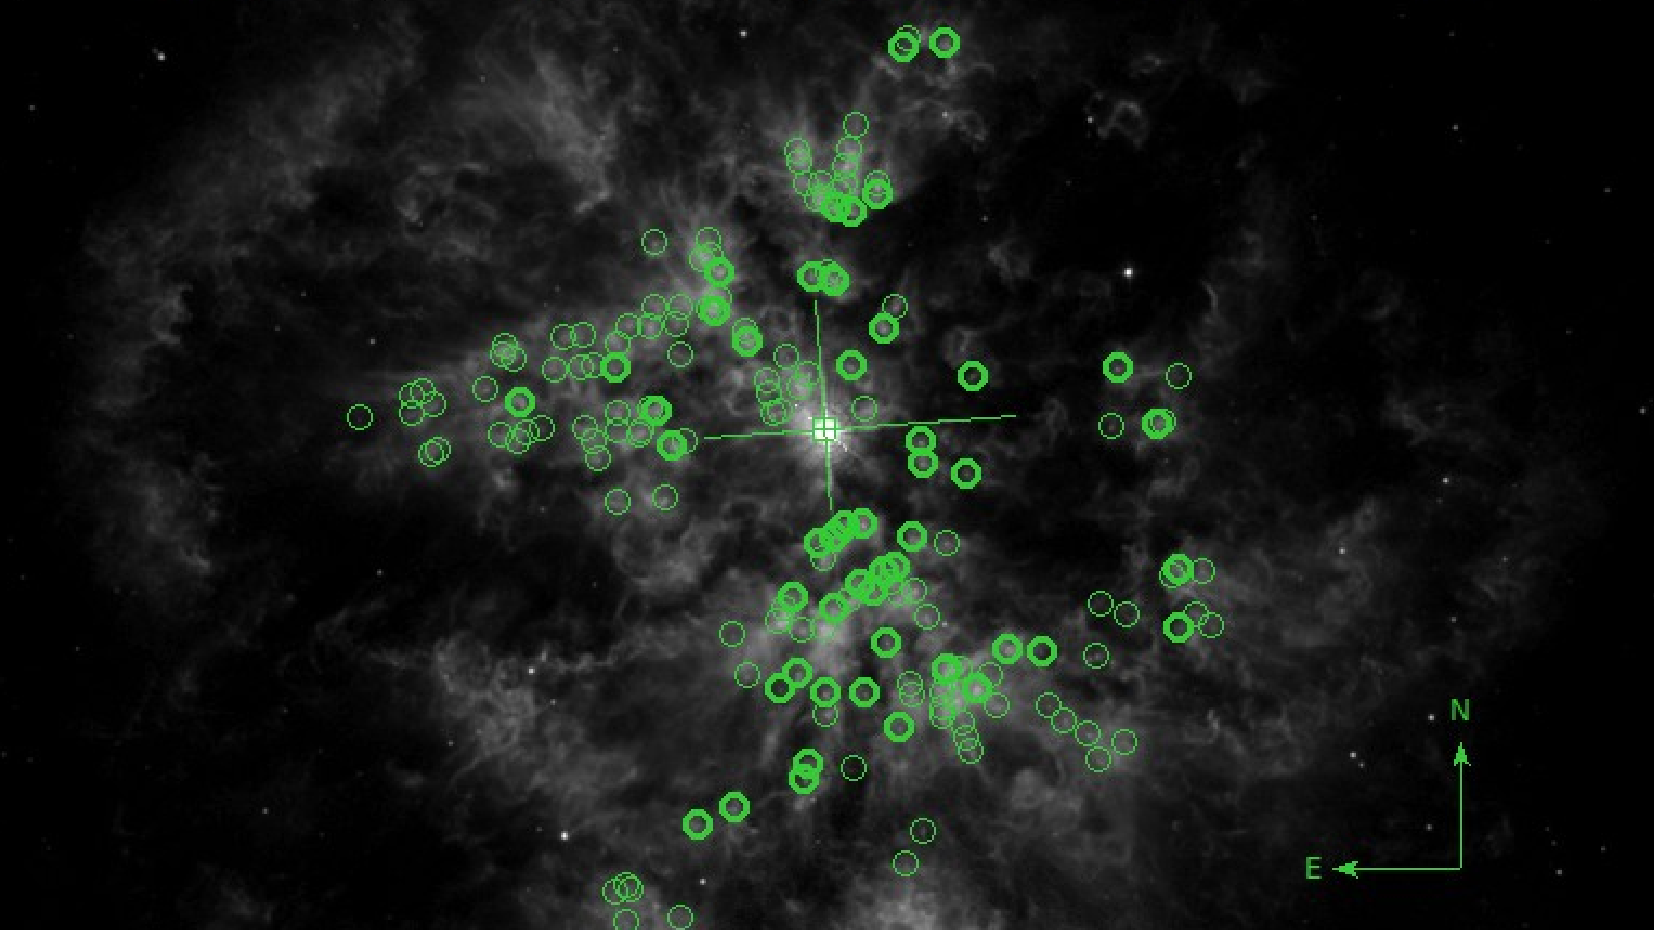
\includegraphics[width=\textwidth]{ultimas correcciones/M167_glo.pdf}
    \end{subfigure}
    \begin{subfigure}[b]{0.45\linewidth}
        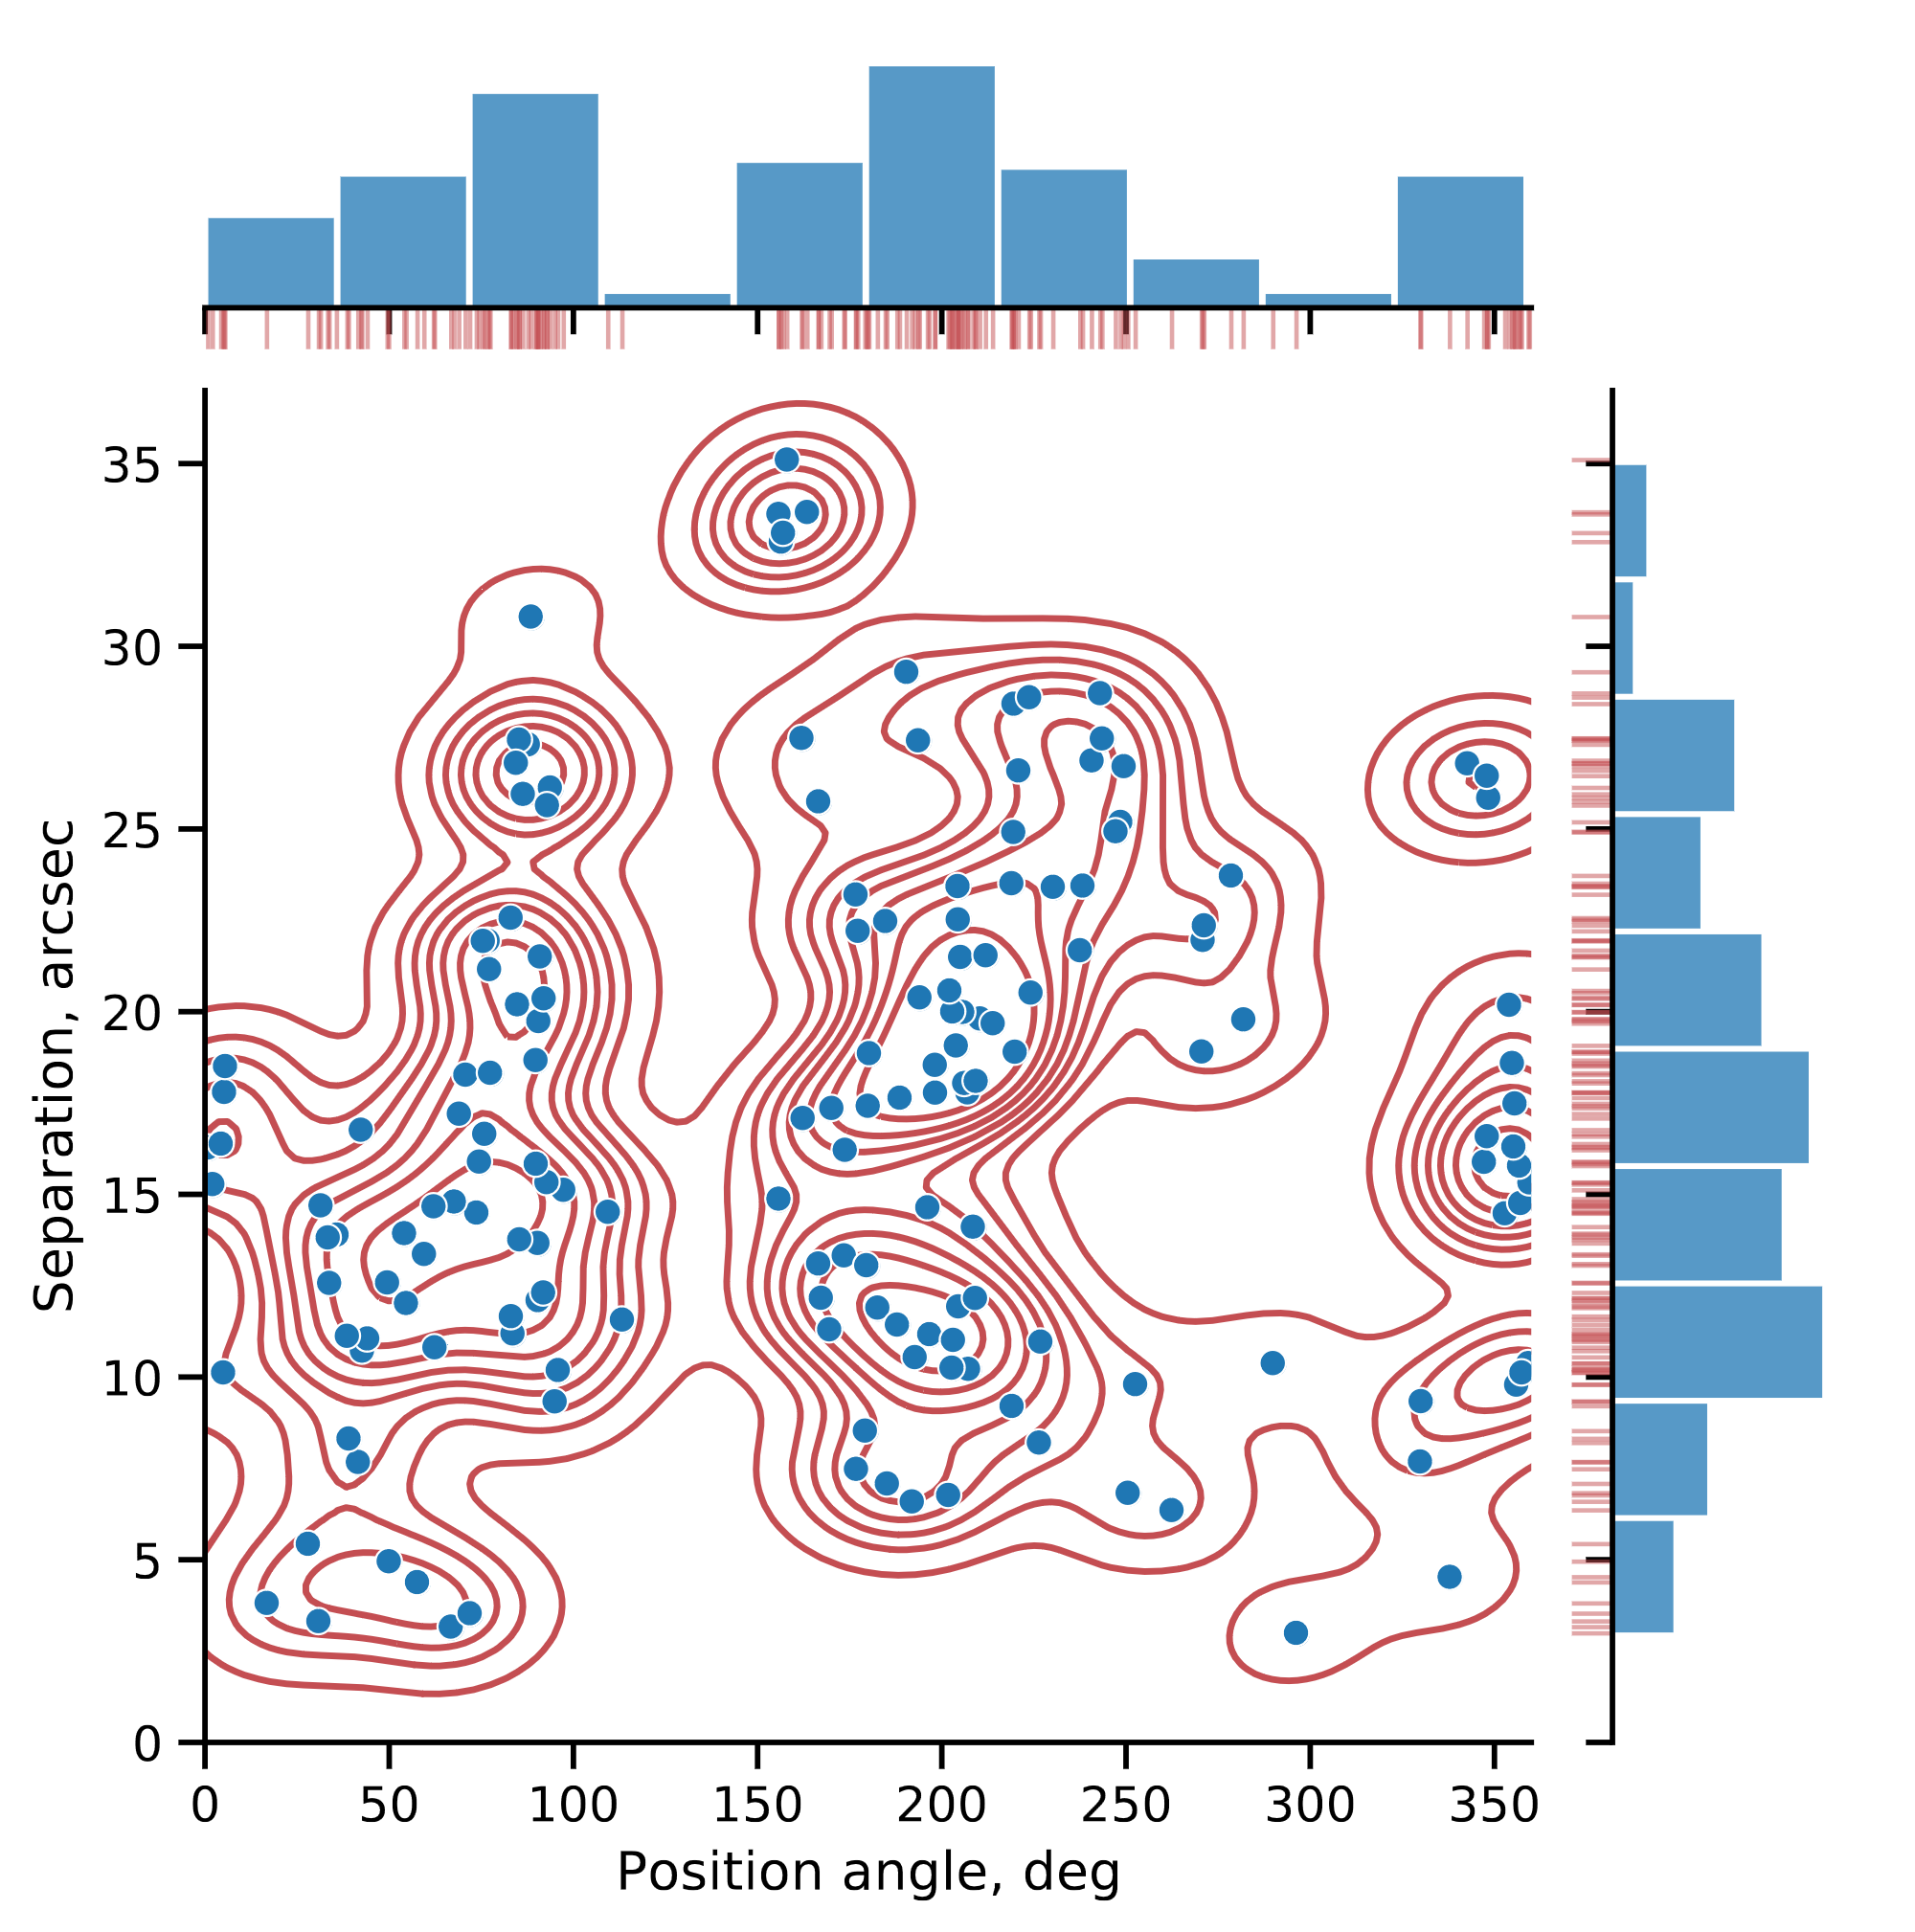
\includegraphics[width=\textwidth]{images Chapter 2/C2_nudos_distribucion.png}
    \end{subfigure}
    \caption{Left: positions of the globules in the M1-67 nebula (green
      points). The red line is the reference used to define the
      angular position of each globule. Right: distribution of the
      globules (blue points) as a function of separation and angular
      position. The upper panel shows the histogram of angular
      positions, while the right panel shows the histogram of
      separations. The red contours are smoothed density isocontours
      of the point distribution.}
    \label{fig:dis_nudos}
\end{figure}

Figure \ref{fig:filters WR124} shows a variety of globules in a small
region, illustrating the different morphologies they present in
different filters.

As noted earlier, the interaction between the globules’
photoevaporative flows and the stellar wind produces a shocked shell,
which we can see owing to recombinations, appearing as emission in
some filters. For example, the shocked shells around the globules are
visible in the HST F656N filter and in the JWST F090W and F444W
filters. We also constructed composite images to isolate the emission
from ionized gas (see Appendix \ref{AP: combos}). In the ionized-gas
image, the shocked shell is more clearly visible.

In the JWST F1130W filter we can see what appear to be parts of the
globule tails. Some appear smaller than others. In some cases, when
globules are very close together, their tails seem to merge, and in
some instances the tails appear to interact with other globules. In
this filter we can also faintly see what may be the interaction
between the ionized gas flow and the stellar wind.

We also created a composite to isolate the emission from neutral gas
(see Appendix \ref{AP: combos}). In this case the morphology of the
globules is revealed more clearly, allowing us to better determine
their properties.

With the wide variety of images available we can make many
comparisons, viewing the globules in different filters and at
different resolutions, which offers several advantages. For example,
JWST observations provide higher spatial resolution, whereas the HST
F656N filter, being very narrow, is less affected by stellar emission,
unlike the JWST observations.

\begin{figure}[htb]
    \centering
    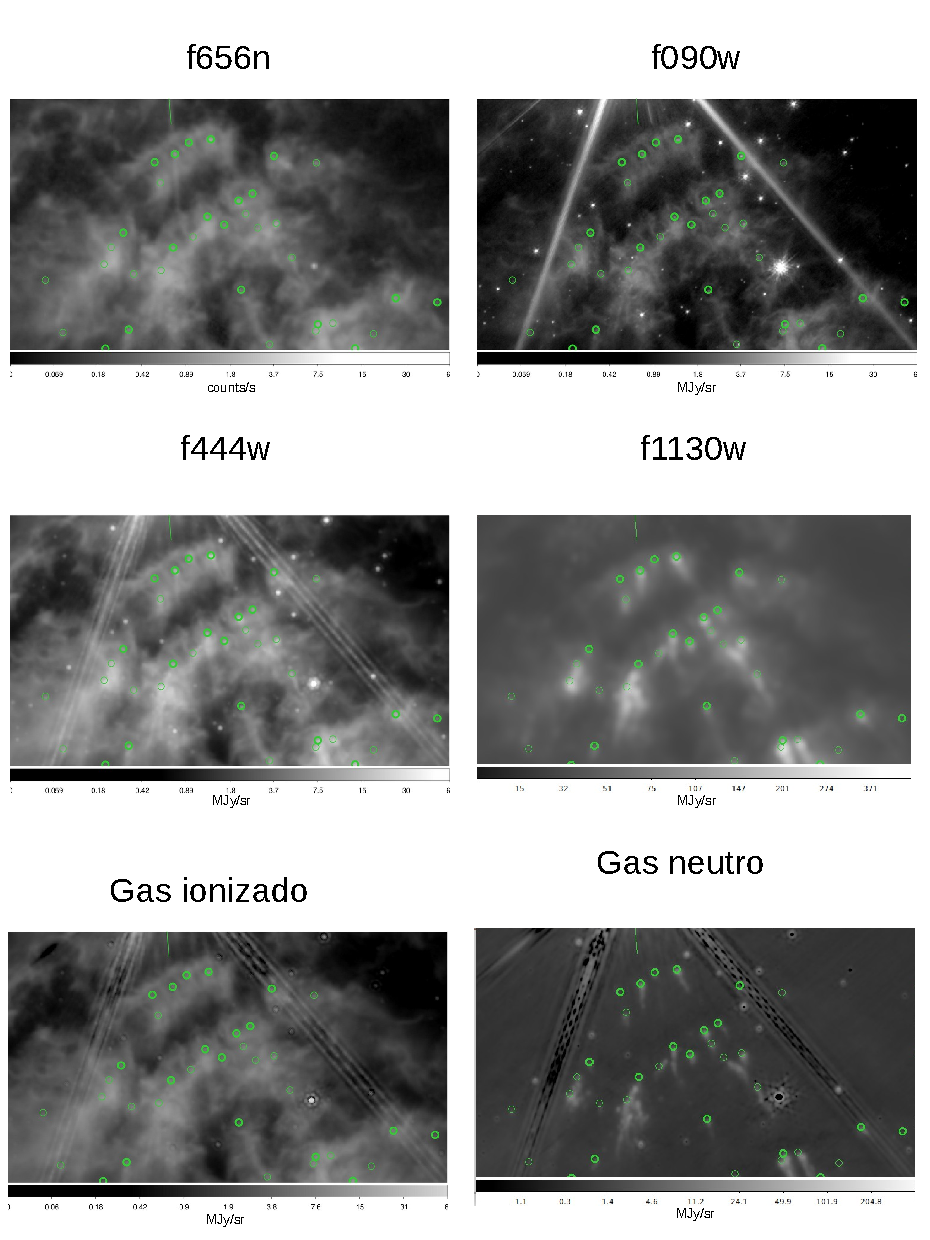
\includegraphics[width=\textwidth]{imagenes_corregidas/Arreglo_04.pdf}
    \caption{Top left: HST image of H$\alpha$ emission with the F656N
      filter. The other panels are JWST images with different filters.
      For ionized gas the following composite was used:
      f44w-0.43\,f335m-0.16(f150w-0.6\,f210m). For neutral gas the
      composite used was
      1.4(f150w-0.6\;f210m)+f335m-0.95\;f210m. Green circles mark the
      globules.}
    \label{fig:filters WR124}
  \end{figure}
  
% \section{Estimando la presión RAM del viento estelar}

% Para este trabajo solo vamos a considerar la presión RAM del viento
% estelar por parte de la estrella WR 124 como la única presión externa
% de confinamiento para las cáscaras chocadas de interacción de los
% glóbulos, la cual la vamos a tomar como
% \begin{equation}
%  P_\mathrm{RAM}= \frac{\dot{M}v_\infty}{4\pi R^2}    
% \end{equation}
% donde $\dot{M}$ es la tasa de pérdida de masa de la estrella,
% $v_\infty$ la velocidad terminal del viento y $R$ la distancia del glóbulo
% a la estrella. Los dos primeros datos están dados en la tabla
% \ref{tab:parametros WR-124} y para $R$ vamos a considerar el rango de
% separación de 0.1--\SI{0.9}{pc}, esto ya que las separaciones entre los
% glóbulos y la estrella caen en este rango considerando que
% \begin{equation}
%     \Big[\frac{R}{\mathrm{UA}}\Big] = \Big[\frac{D}{\mathrm{pc}}\Big]\,\Big[\frac{\theta}{\mathrm{arcsec}}\Big],
% \end{equation}
% donde $\theta$ es la separación que medimos directamente de las
% observaciones en arcsec y $D$ es la distancia de nosotros a la
% estrella. En la Figura \ref{P_RAM} vemos como es esta presión RAM del
% viento como función de la distancia.

% \begin{figure}[htb]
%     \centering    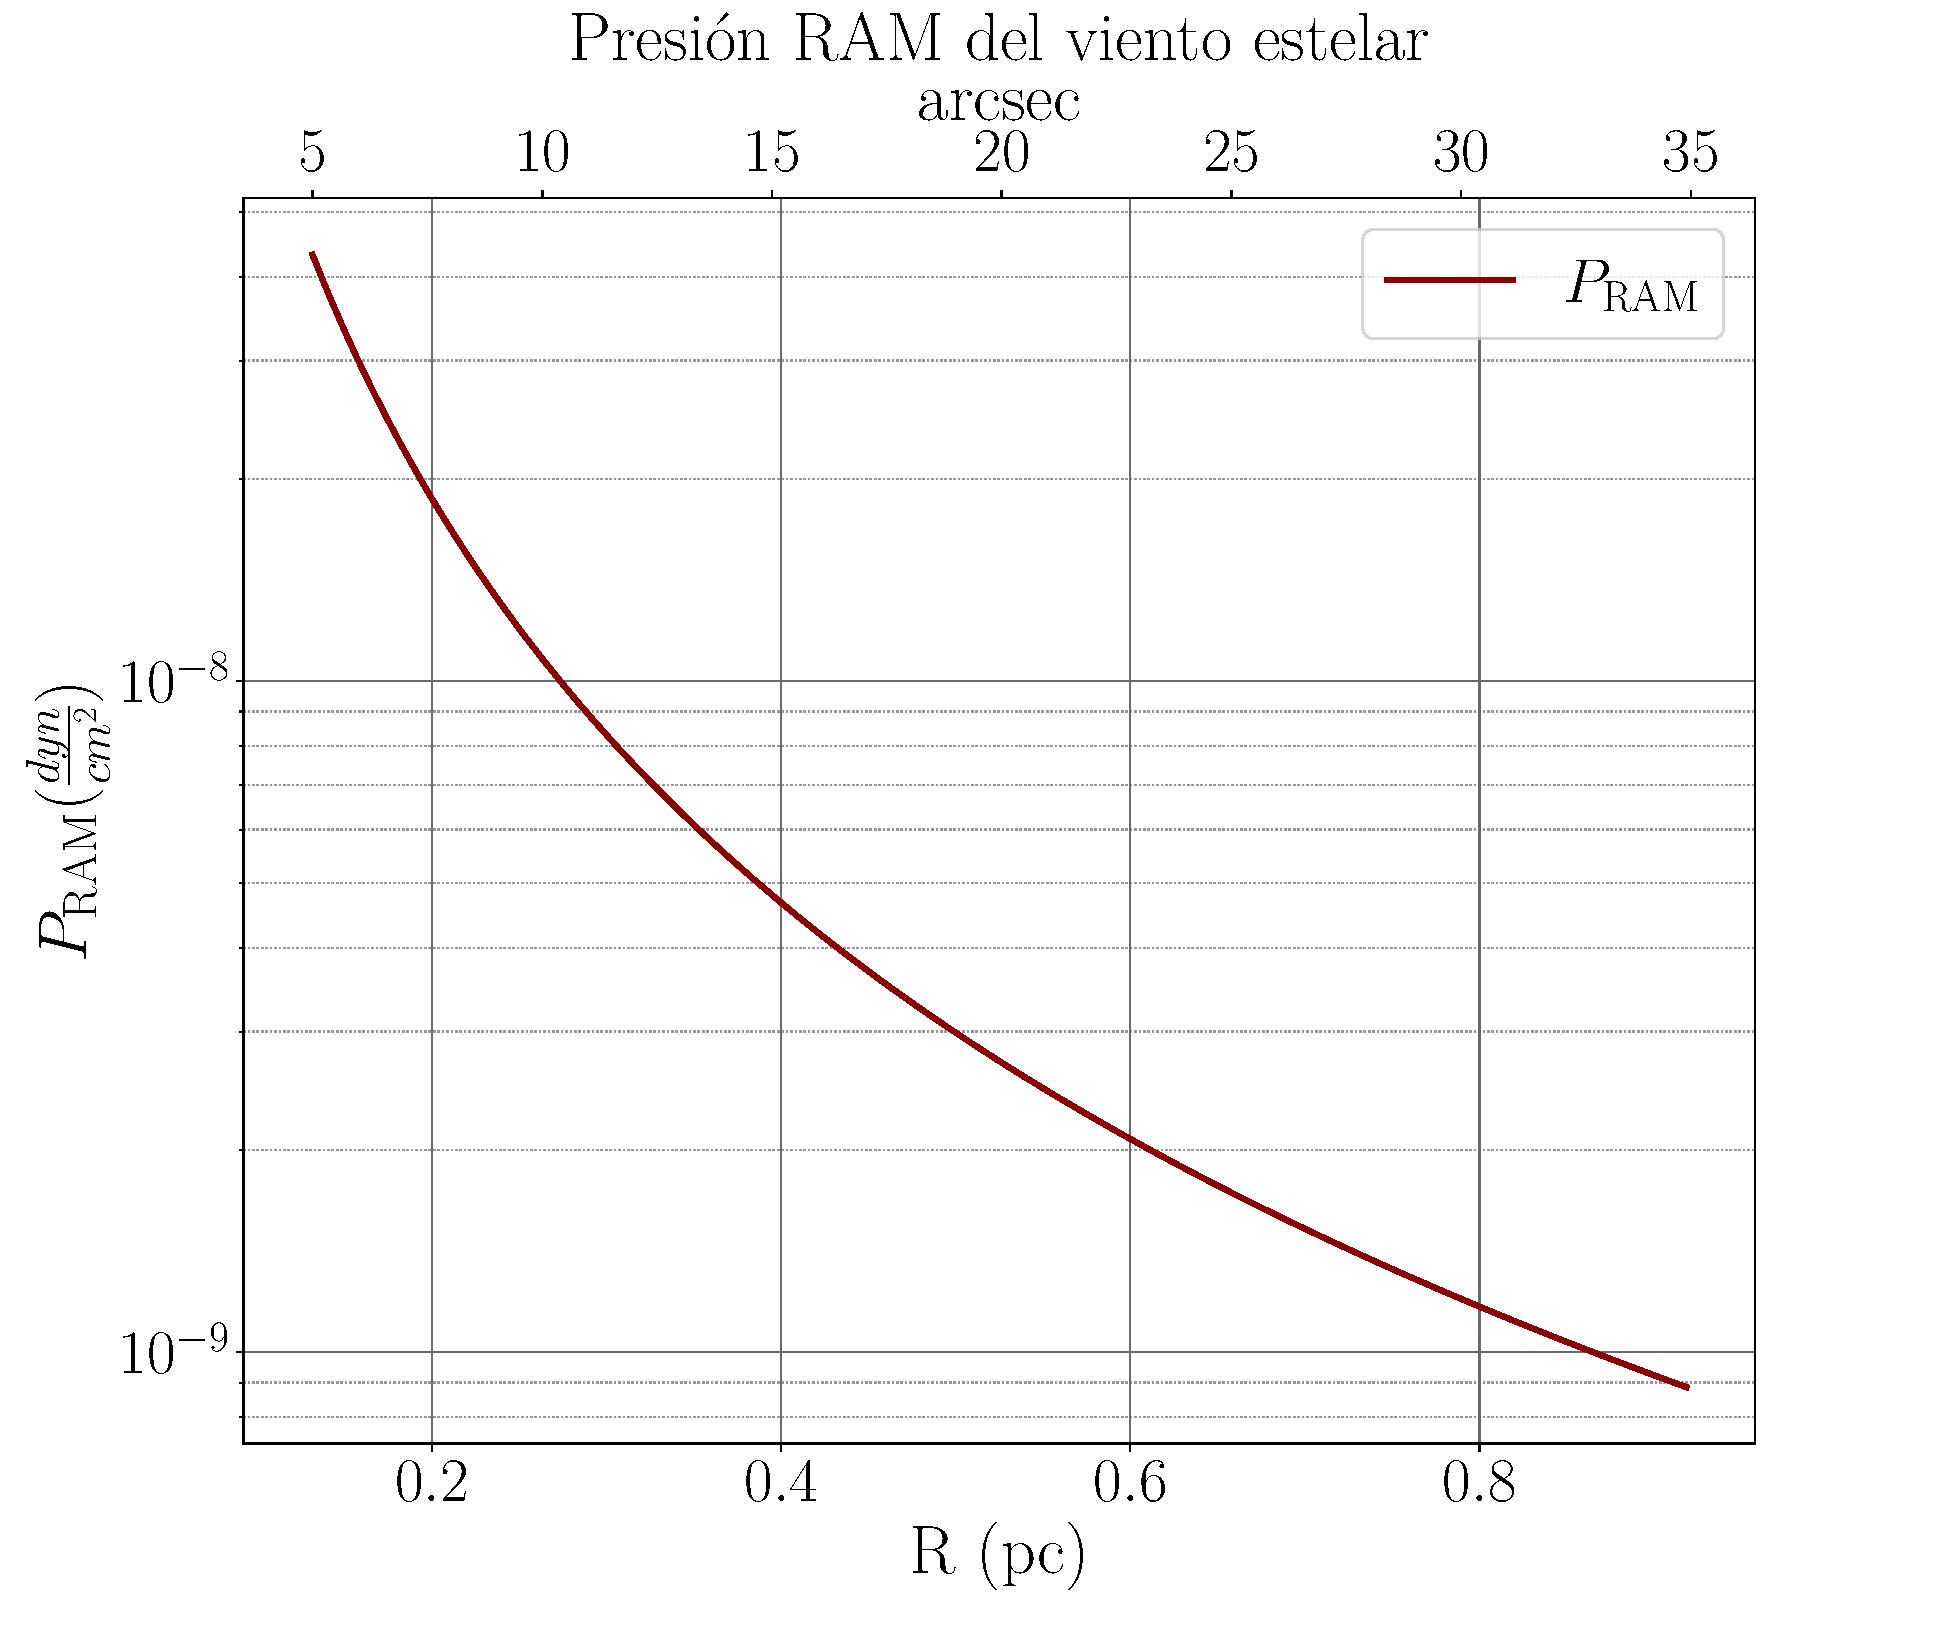
\includegraphics[width=\textwidth]{Nuevas imagenes finales/PRAMcgs_n.pdf}
%     \caption{Presión RAM del viento estelar de la estrella WR 124 como función de la distancia en parsec}
%     \label{P_RAM}
% \end{figure}

  \section{Estimating the RAM pressure of the stellar wind}

In this work we consider only the RAM pressure of the stellar wind
from WR~124 as the external confining pressure for the shocked shells
surrounding the interacting globules. We write this as
\begin{equation}
 P_\mathrm{RAM}= \frac{\dot{M}v_\infty}{4\pi R^2},    
\end{equation}
where $\dot{M}$ is the stellar mass-loss rate, $v_\infty$ the terminal
wind velocity, and $R$ the distance from the globule to the star. The
first two parameters are given in Table \ref{tab:parametros WR-124},
and for $R$ we consider the separation range 0.1--\SI{0.9}{pc}, since
the measured separations of the globules from the star fall within
this interval. The distance is obtained as
\begin{equation}
    \Big[\frac{R}{\mathrm{AU}}\Big] = \Big[\frac{D}{\mathrm{pc}}\Big]\,\Big[\frac{\theta}{\mathrm{arcsec}}\Big],
\end{equation}
where $\theta$ is the angular separation measured directly from the
observations and $D$ is the distance from us to the star. Figure
\ref{P_RAM} shows how the RAM pressure of the stellar wind varies as a
function of distance.

\begin{figure}[htb]
  \centering    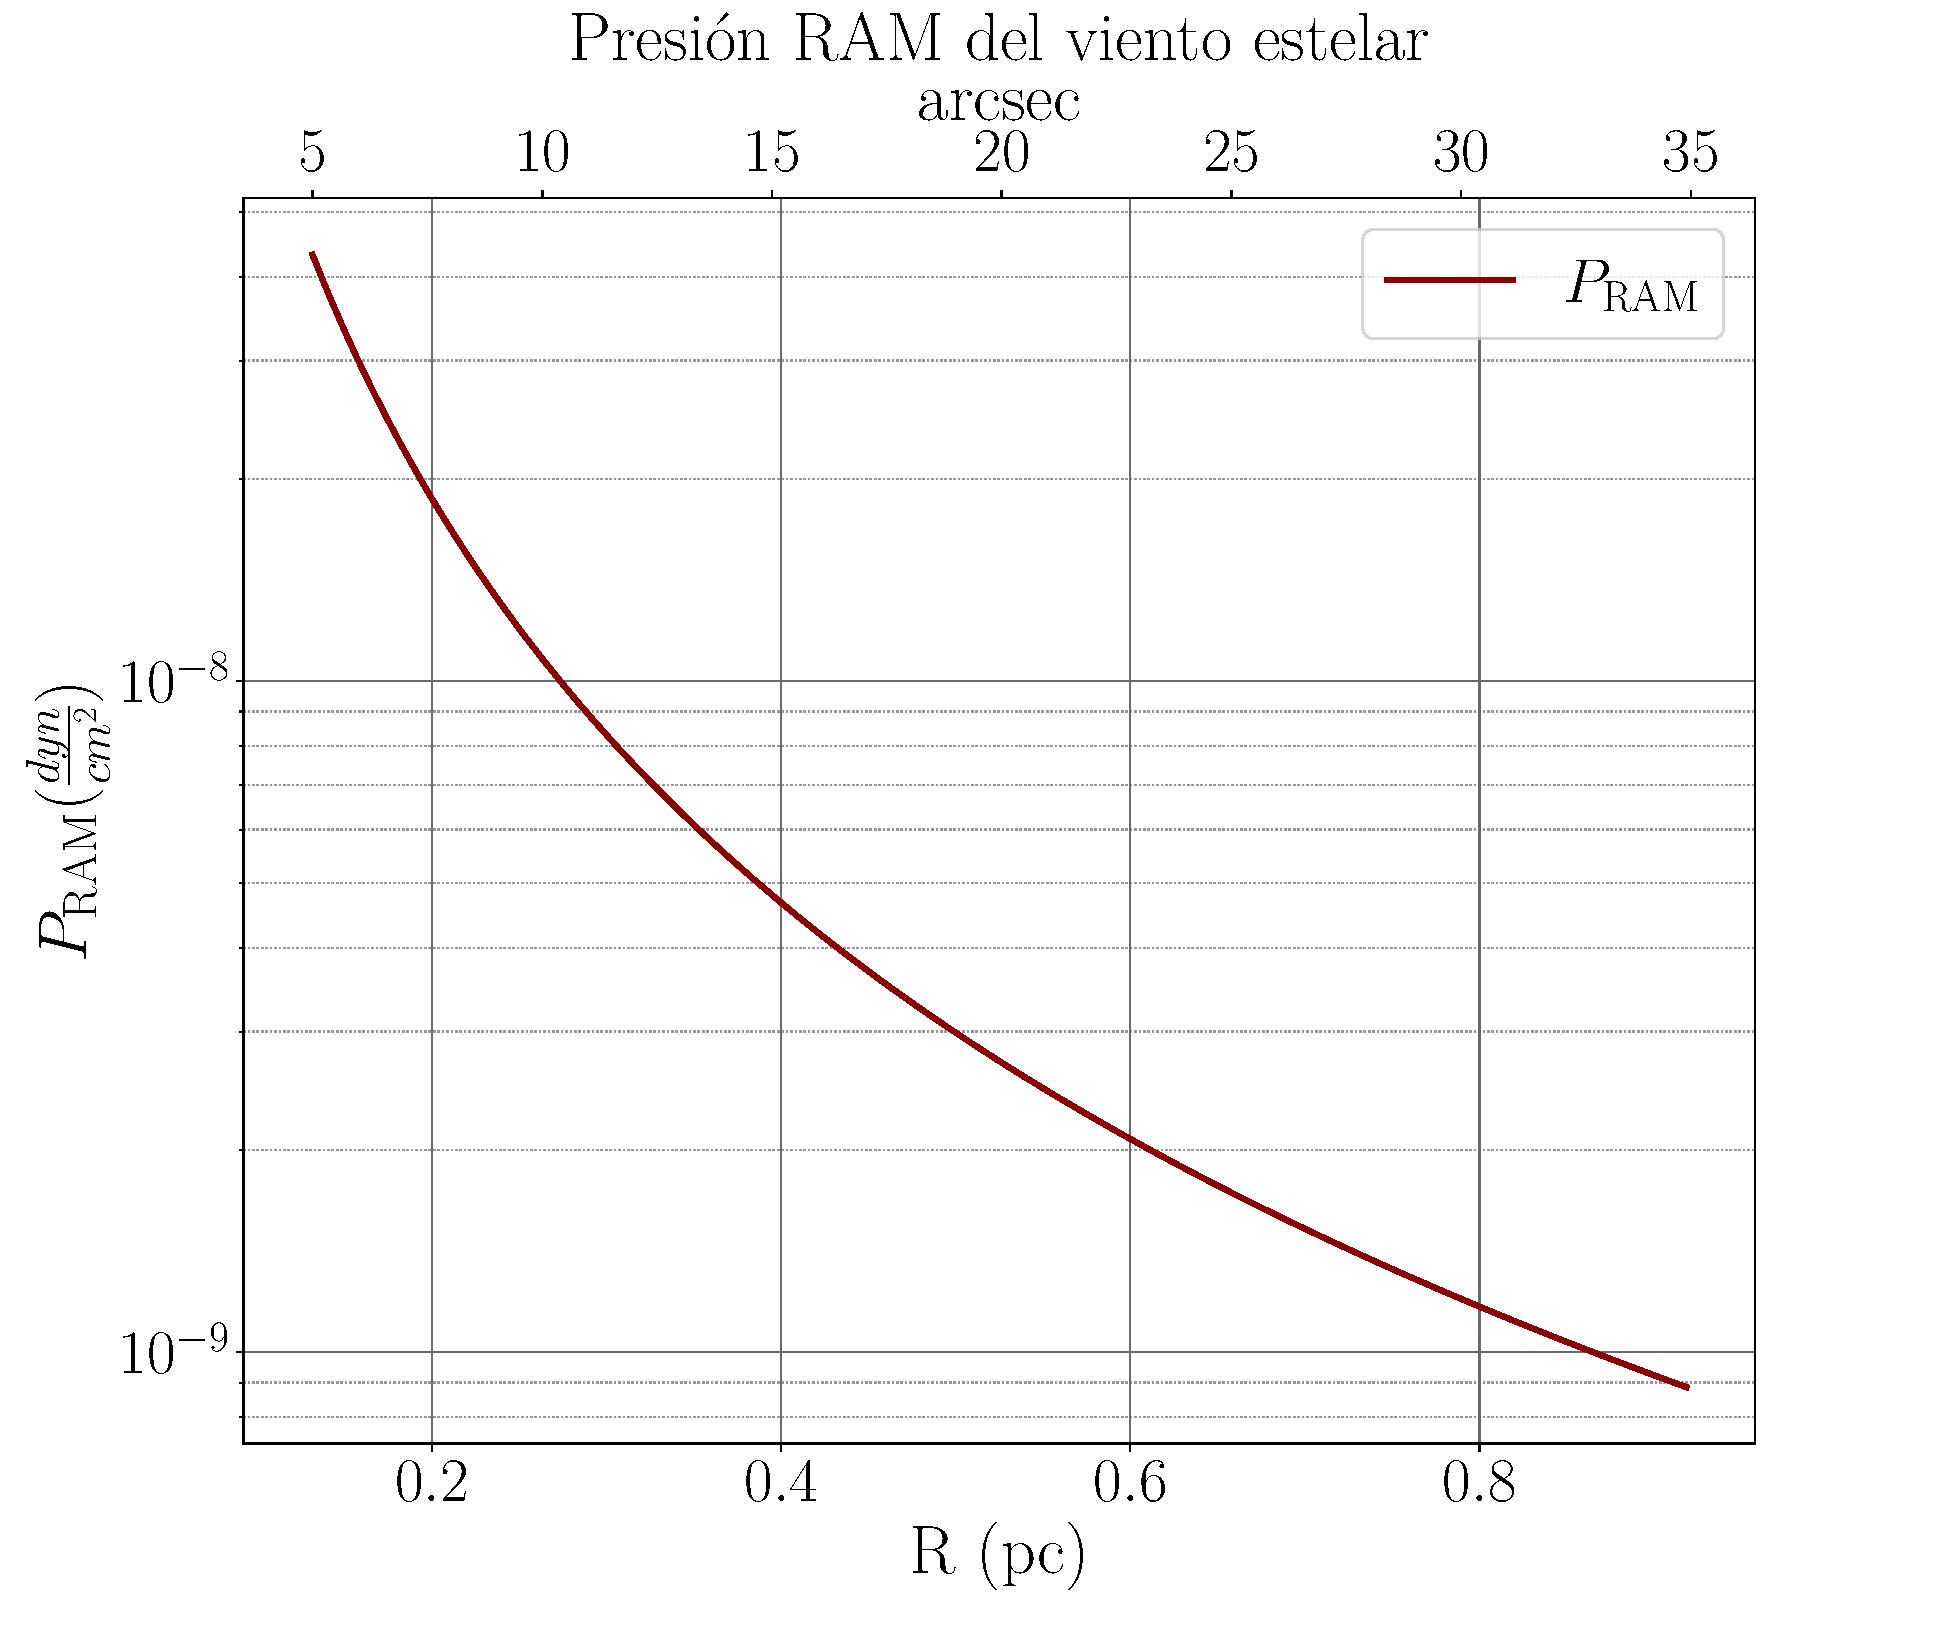
\includegraphics[width=\textwidth]{Nuevas imagenes finales/PRAMcgs_n.pdf}
  \caption{RAM pressure of the stellar wind from WR~124 as a function
    of distance in parsecs.}
  \label{P_RAM}
\end{figure}


  
\chapter{Model fitting to brightness profiles}
\chaptermark{Model fitting}\label{Chapter : Ajuste}

In this chapter we use the various observations to measure the sizes
of the globules, their shocked shells, and the widths of those shells.
We can also measure the brightness at the center of the globule and in
the shocked shell, which will later allow us to estimate the density
of the ionized gas in the shocked shell.

The measurements of the different parameters for the 168 identified
globules are carried out as follows. Once the globule positions are
known, we locate the peak of H$\alpha$ emission, which we define as the
center of the globule\footnote{In the ionized-gas observations we have
only an estimate of the globule size; in Section \ref{Sec : radio
  neutro} we obtain a more realistic measurement of the globule size
using neutral gas.}. We then define the symmetry axis of the model
(Figure \ref{fig:zones}) as the line connecting the center of the
globule with the star. Since our main interest is to describe the
globule and its shocked shell, we apply a mask to isolate these two
components. This mask ensures that our measurements are not affected
by the complex structure of the nebula or by nearby globules. The mask
is defined as follows: we take only those pixels lying within
\SI{0.2}{\arcsecond} of the globule center, and those within a maximum
distance of \SI{1.5}{\arcsecond} and a maximum angle of $60^\circ$
with respect to the symmetry axis. With these values the globules and
their shocked shells are always included in the mask, and the chosen
parameters yield reliable results for the different measurements.

We then plot the brightness of each pixel within the mask as a
function of distance from the globule center, as shown in Figure
\ref{ejemplo mascara}. To these points we fit two Gaussians and a
constant.

\begin{figure}[htb]
  \begin{subfigure}[b]{0.5\textwidth}
    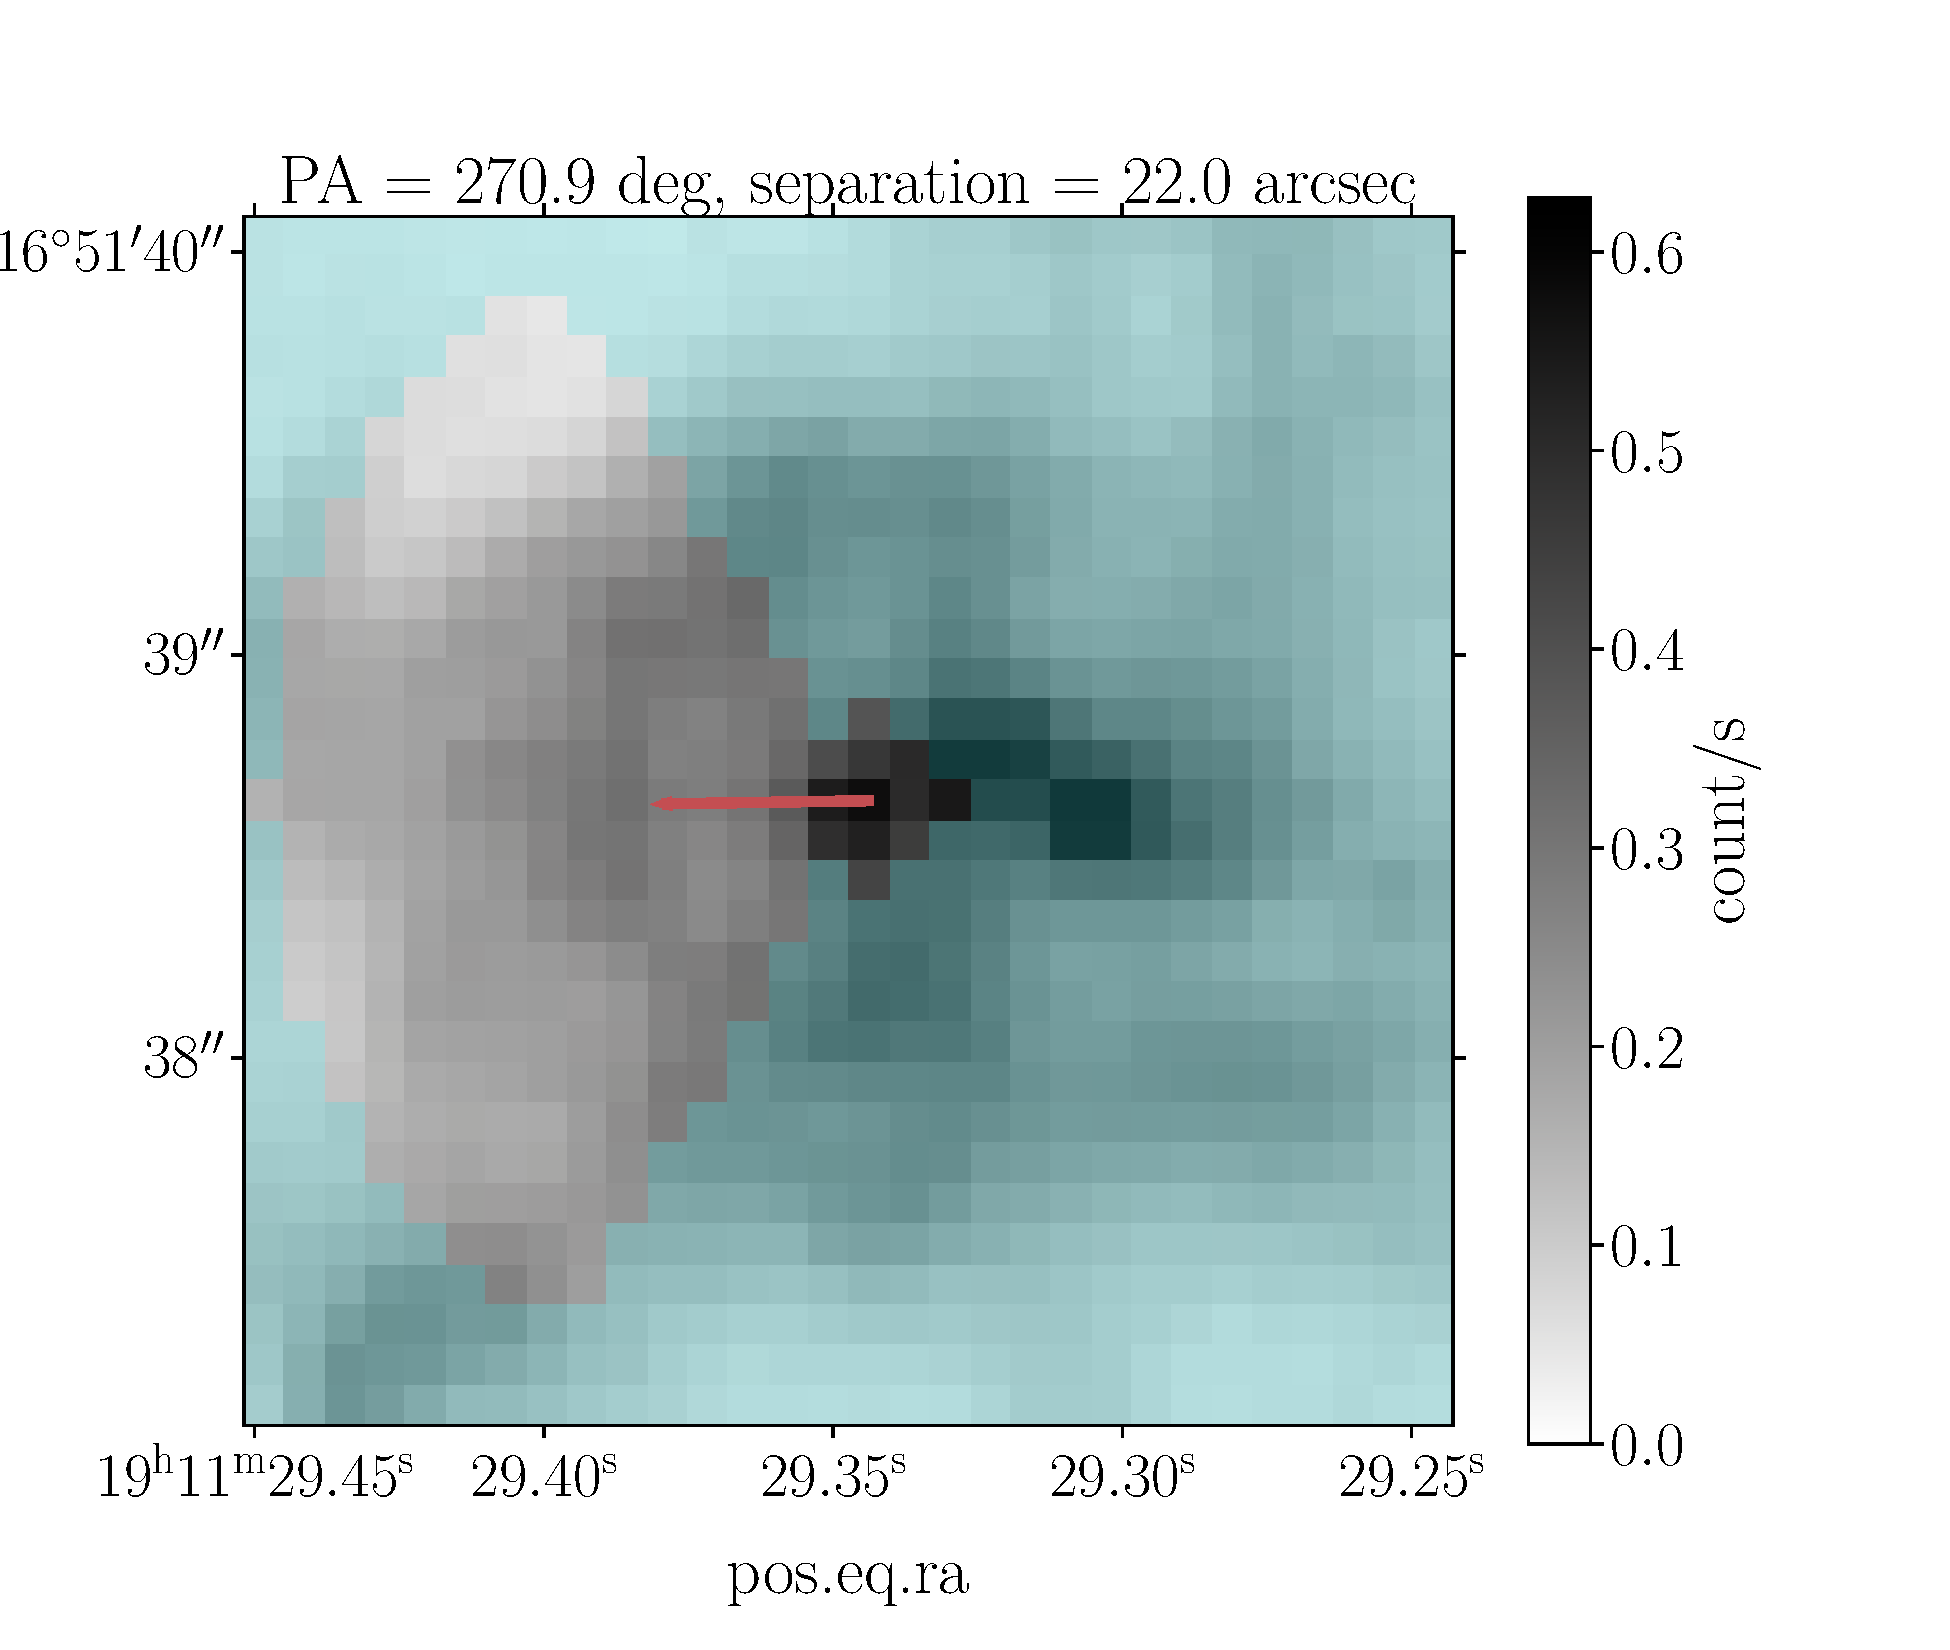
\includegraphics[width=\textwidth, height=0.9\textwidth]{Nuevas imagenes finales/F_4_1_A.pdf}
    \caption{Example of a mask used for the globules. The mask is
      defined by the gray-scale pixels.}
    \label{fig:f1}
  \end{subfigure}
  \hfill
  \begin{subfigure}[b]{0.5\textwidth}
    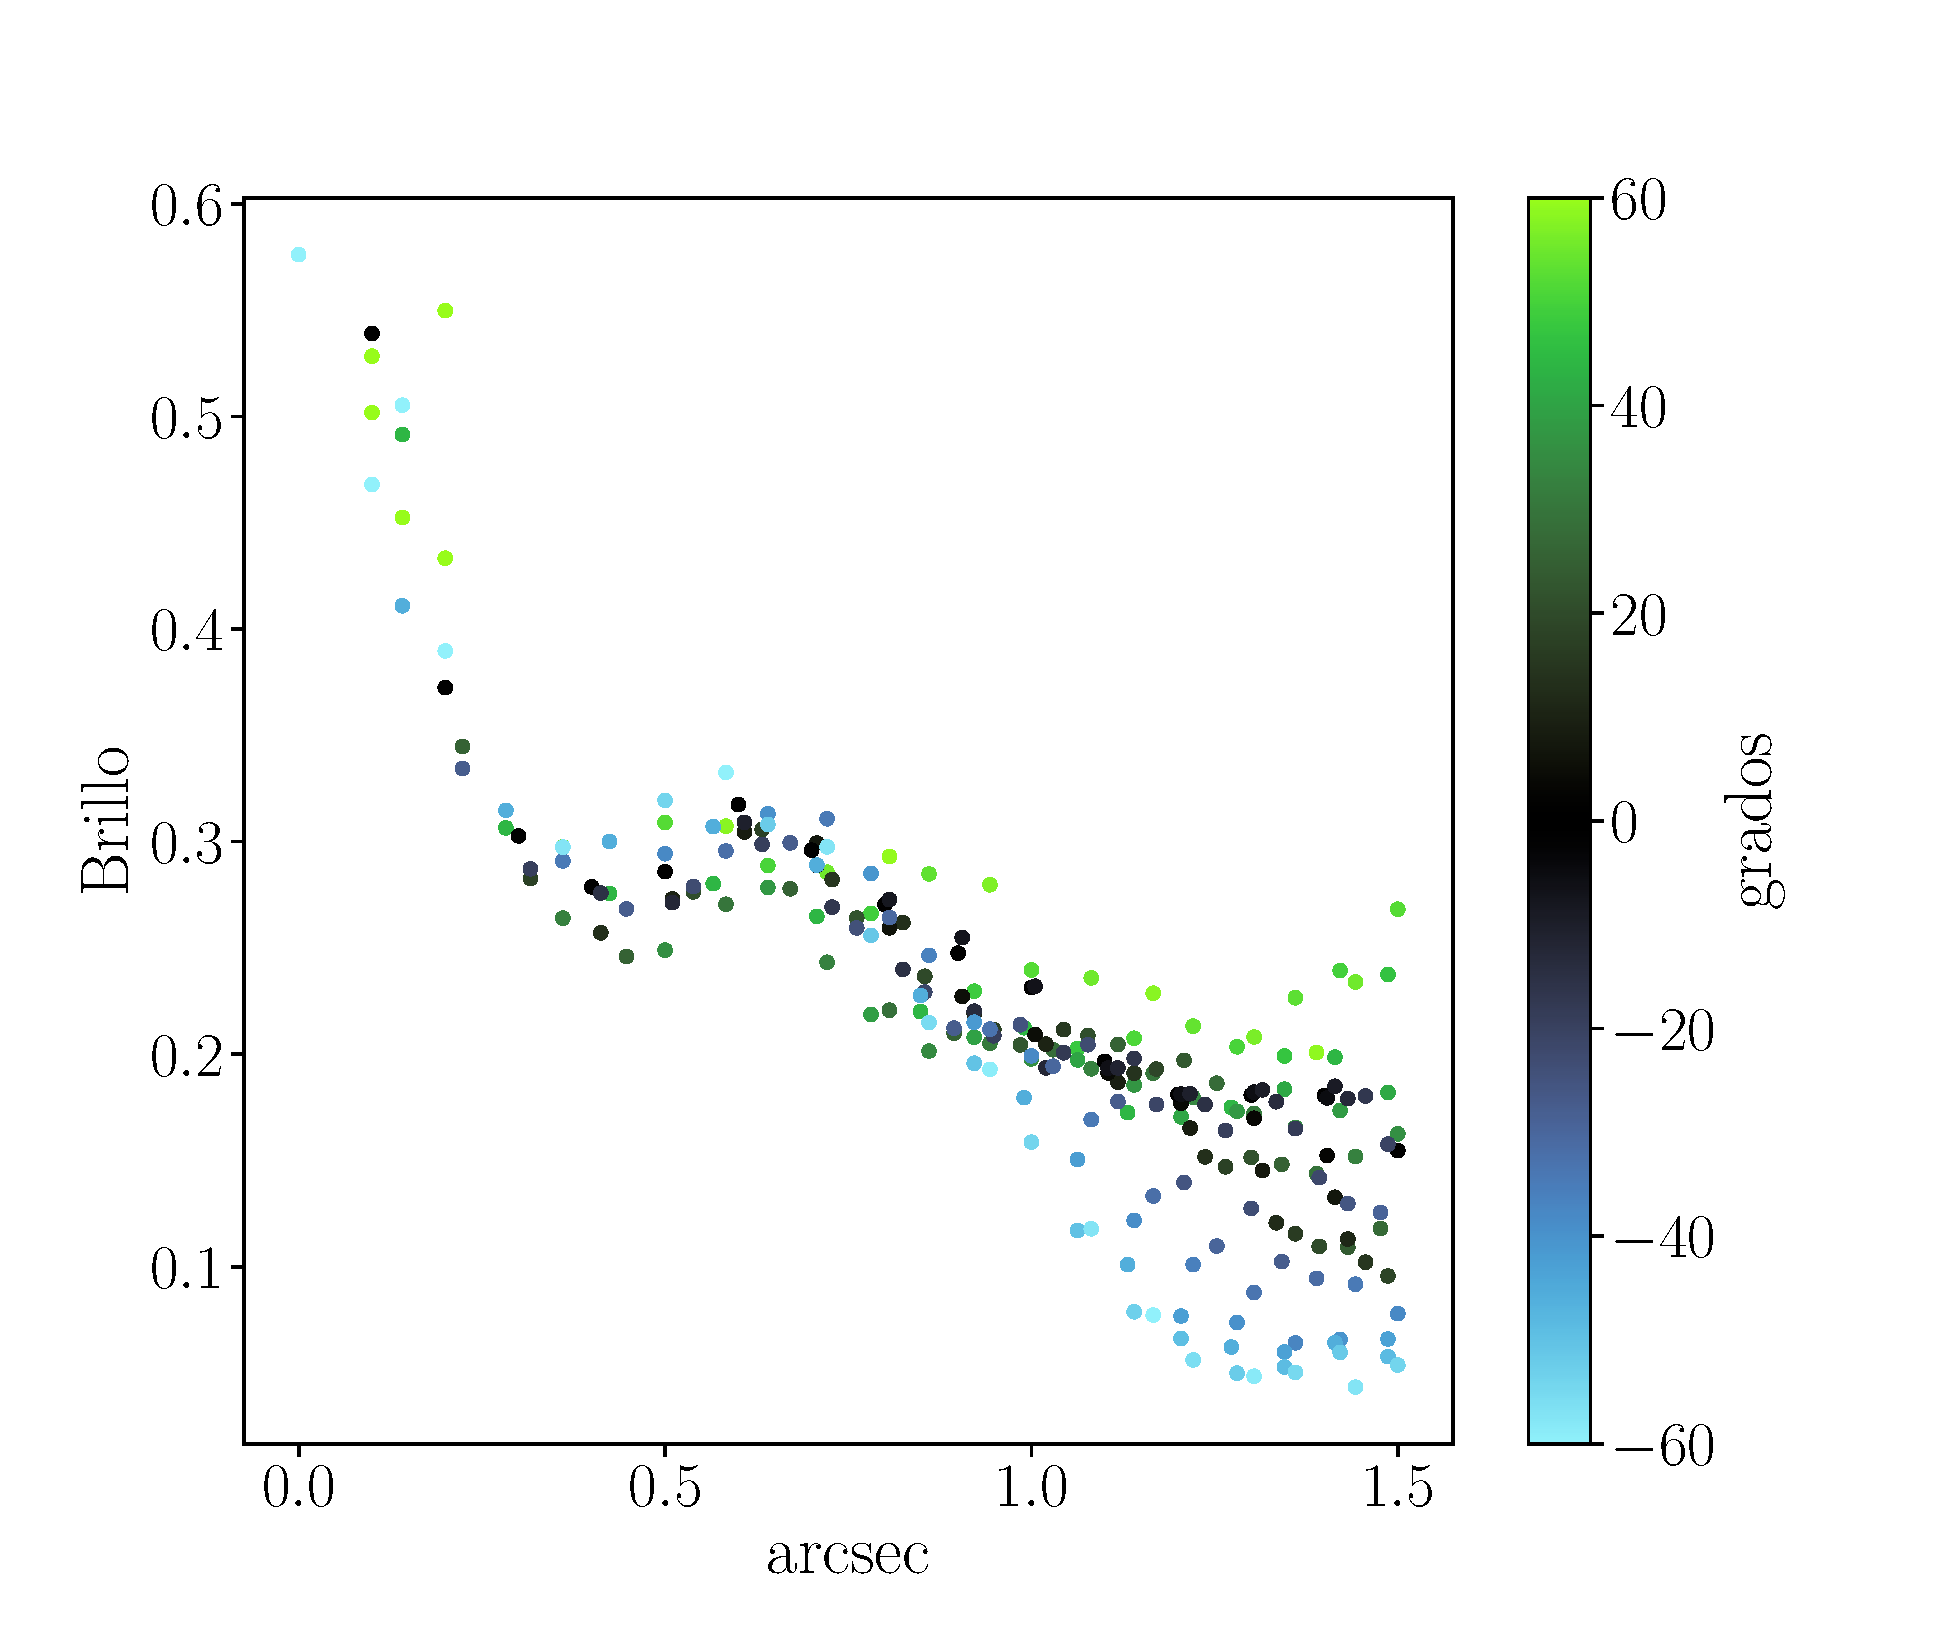
\includegraphics[width=\textwidth, height=0.9\textwidth]{Nuevas imagenes finales/F_4_1_B.pdf}
    \caption{Brightness within the mask as a function of distance from
      the globule center, measured along the symmetry axis.}
    \label{fig:f2}
  \end{subfigure}
  \caption{Left: example of the mask used for fitting brightness
    profiles (gray-scale pixels), here using HST observations. The
    globule center is at the image center. The red line connects the
    globule center to the star (off to the left), defining the
    symmetry axis. Pixels within a circle of \SI{0.2}{\arcsecond}
    around the globule center are included, as well as those within
    \SI{1.5}{\arcsecond} and within $60^\circ$ of the symmetry axis.
    Right: brightness of the pixels included in the mask as a function
    of distance from the globule center and angle with respect to the
    symmetry axis. Green points correspond to pixels in the lower part
    of the left panel, blue points to pixels in the upper part within
    the mask.}
  \label{ejemplo mascara}
\end{figure}

The fit is motivated as follows. The width of the first Gaussian,
centered at zero, gives the size of the globule, assuming that the
emission peak coincides with the globule center. The second Gaussian
indicates the location and width of the shocked shell. We expect an
emission peak in the shocked shell due to recombinations, hence the
second Gaussian. The distance between the peaks of the two Gaussians
gives the radius of the shocked shell. Finally, the constant
represents the mean background brightness in the region. In the fit we
assign lower weight to pixels farther from the globule center and to
those with larger angle from the symmetry axis, according to
\begin{equation}\label{eq: peso}
    w = \frac{\cos^2(\theta)}{(0.3+r)^2},
\end{equation}
where $\theta$ is the angle relative to the symmetry axis and $r$ is
the distance from the globule center. The fit is performed with the
\verb|fitting.LevMarLSQFitter|\footnote{Documentation:
  \url{https://docs.astropy.org/en/latest/api/astropy.modeling.fitting.LevMarLSQFitter.html}}
package of \verb|astropy.modeling|. A clearer example of these fits is
shown in Figure \ref{ejemplo ajuste}.

\begin{figure}[htbp]
    \centering
    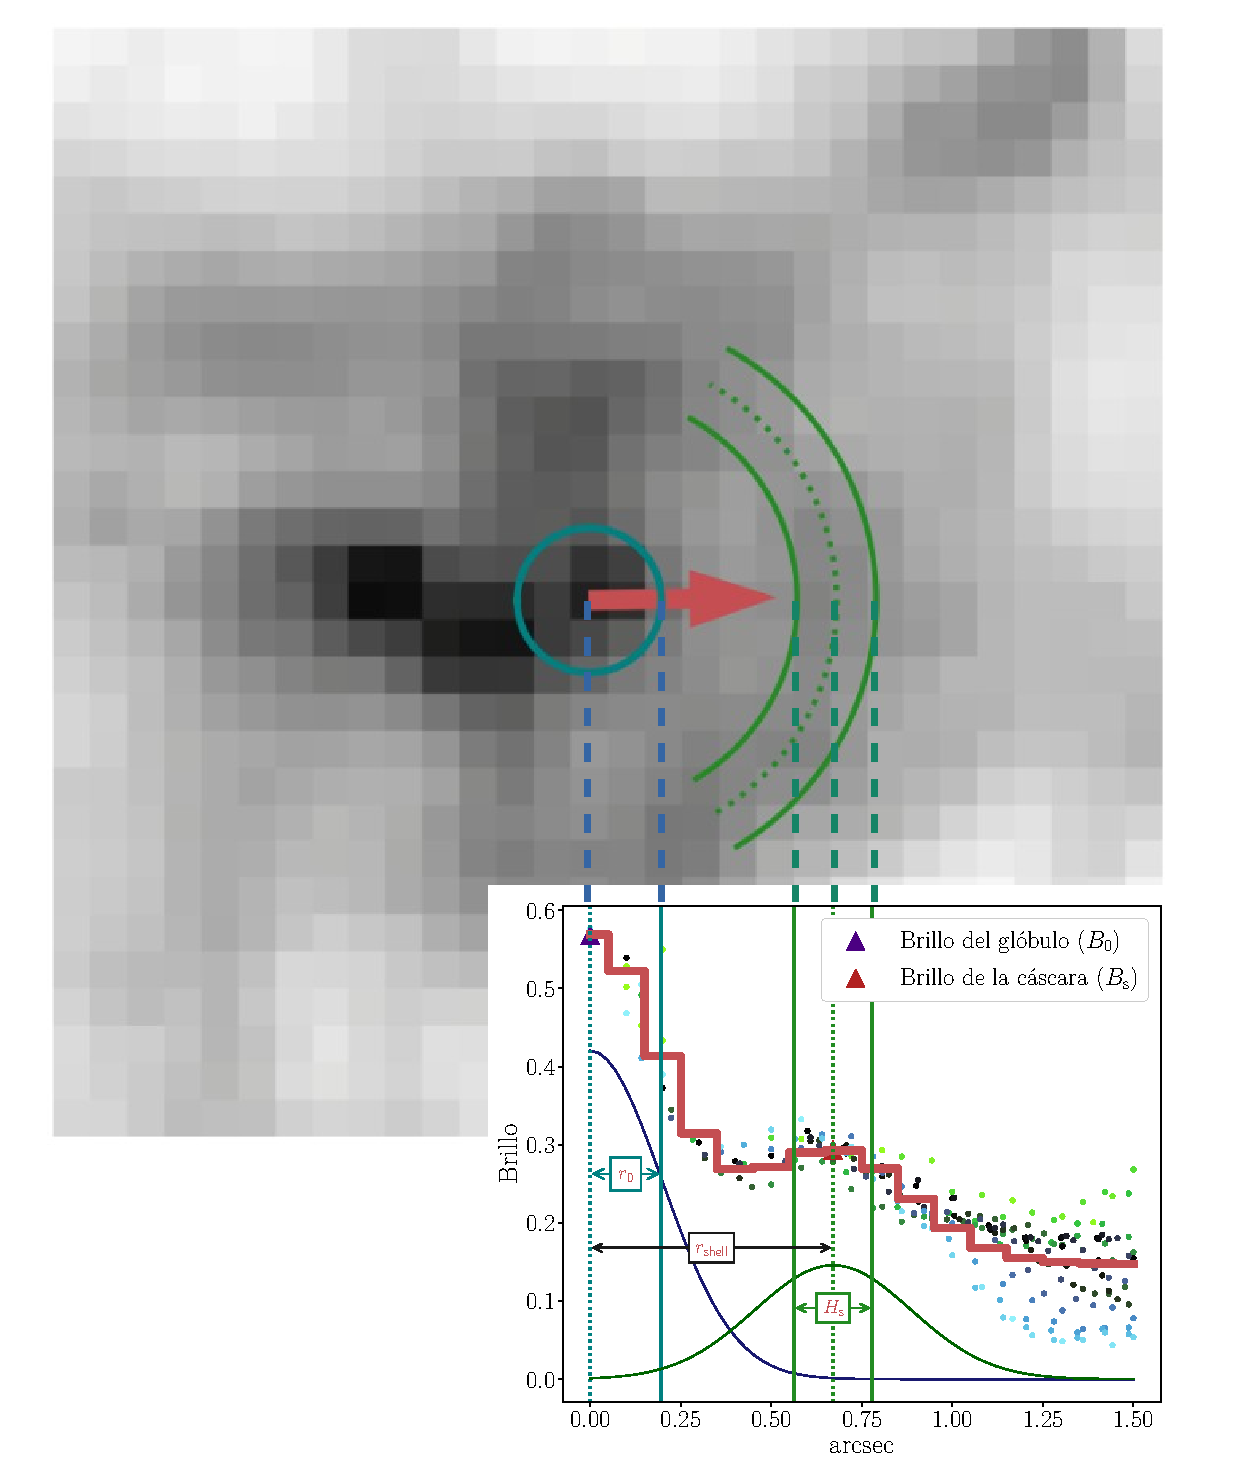
\includegraphics[width=\textwidth]{imagenes_corregidas/Ejemplo_ajuste_final.pdf}
    \caption{Example of the fit of two Gaussians plus a constant to
      the brightness profiles. This example is the same as in Figure
      \ref{ejemplo mascara}, but for visualization the globule image
      has been rotated $180^\circ$. The internal and shell brightness
      values correspond to the peaks of the first and second
      Gaussians, respectively. The $\sigma$ of the first Gaussian
      centered at zero gives the size of the inner region. The shell
      width is obtained from the $\sigma$ of the second Gaussian. The
      shell radius is taken as the distance between the peaks of the
      two Gaussians. This fit is applied to the HST observations, and
      the figure shows how the fit appears directly on the image.}
    \label{ejemplo ajuste}
\end{figure}

The fitting procedure was applied to the HST observations and, for the
JWST, to the F090W filter and to the composite image isolating ionized
gas. In this way we obtained several independent measurements at
different resolutions, providing greater confidence that we are indeed
detecting a shell and measuring the sizes of the different fitted
parameters.

\section{Measuring the radius in the neutral component} 
\label{Sec : radio neutro}

The previous fitting procedure was performed using images of ionized
gas emission, so the measured radii did not accurately represent the
neutral component. To measure the neutral gas we used a combination of
the JWST filters F150W, F210M, and F335M to isolate neutral emission
(see Appendix \ref{AP: combos}). With this combination we avoid
contamination of our measurements by field stars or by shocked shells.

In this case we fit only a Gaussian and a constant to the brightness
profile, since the shocked shell is not visible here. The fitting was
carried out as follows. Given that the mean radius of the globules
from the previous fit was \SI{0.14}{\arcsecond} with a variation of
$\pm\SI{0.04}{\arcsecond}$, we placed a mask of
\SI{0.2}{\arcsecond} around the emission peak together with cones of
small opening angle. These cones are perpendicular to the symmetry
axis of the model and extend \SI{1.5}{\arcsecond}. With this mask we
expect the entire neutral emission to lie within the small circle,
while the cones serve to better constrain the constant background
level, since they are not affected by the wings of the globules.
Figure \ref{Medicion de r_0} shows how the globule falls inside the
mask without contamination from ionized gas emission or field stars.

With these fits we obtain the radius of the globules, $r_0$, the
radius of the shocked shell, $r_\mathrm{shell}$, and the width of the
shocked shell, $H_\mathrm{s}$. Since both $r_0$ and $H_\mathrm{s}$ are
measured using the $\sigma$ of the fitted Gaussian (i.e. the RMS width
of the profile), for comparison with instrumental widths our observed
width is given by
\begin{equation}
    W_\mathrm{obs}= 2\sqrt{2\ln{2}} \, \sigma_\mathrm{obs},
\end{equation}
where $\sigma_\mathrm{obs}$ is the measured value from the
observations. Considering the point spread function (PSF) of each
telescope, the intrinsic width is then
\begin{equation}
    W_\mathrm{real} = \frac{\sqrt{W_\mathrm{obs}^2-\Delta^2}}{2},
\end{equation}
where $\Delta$ is the PSF of the telescope. For HST
$\Delta=\SI{0.067}{\arcsecond}$, and for JWST
$\Delta=\SI{0.145}{\arcsecond}$ (for the filter combination used to
observe only the ionized gas). In this way we obtain more realistic
measurements of these two quantities.

\begin{figure}[htb]
  \centering
  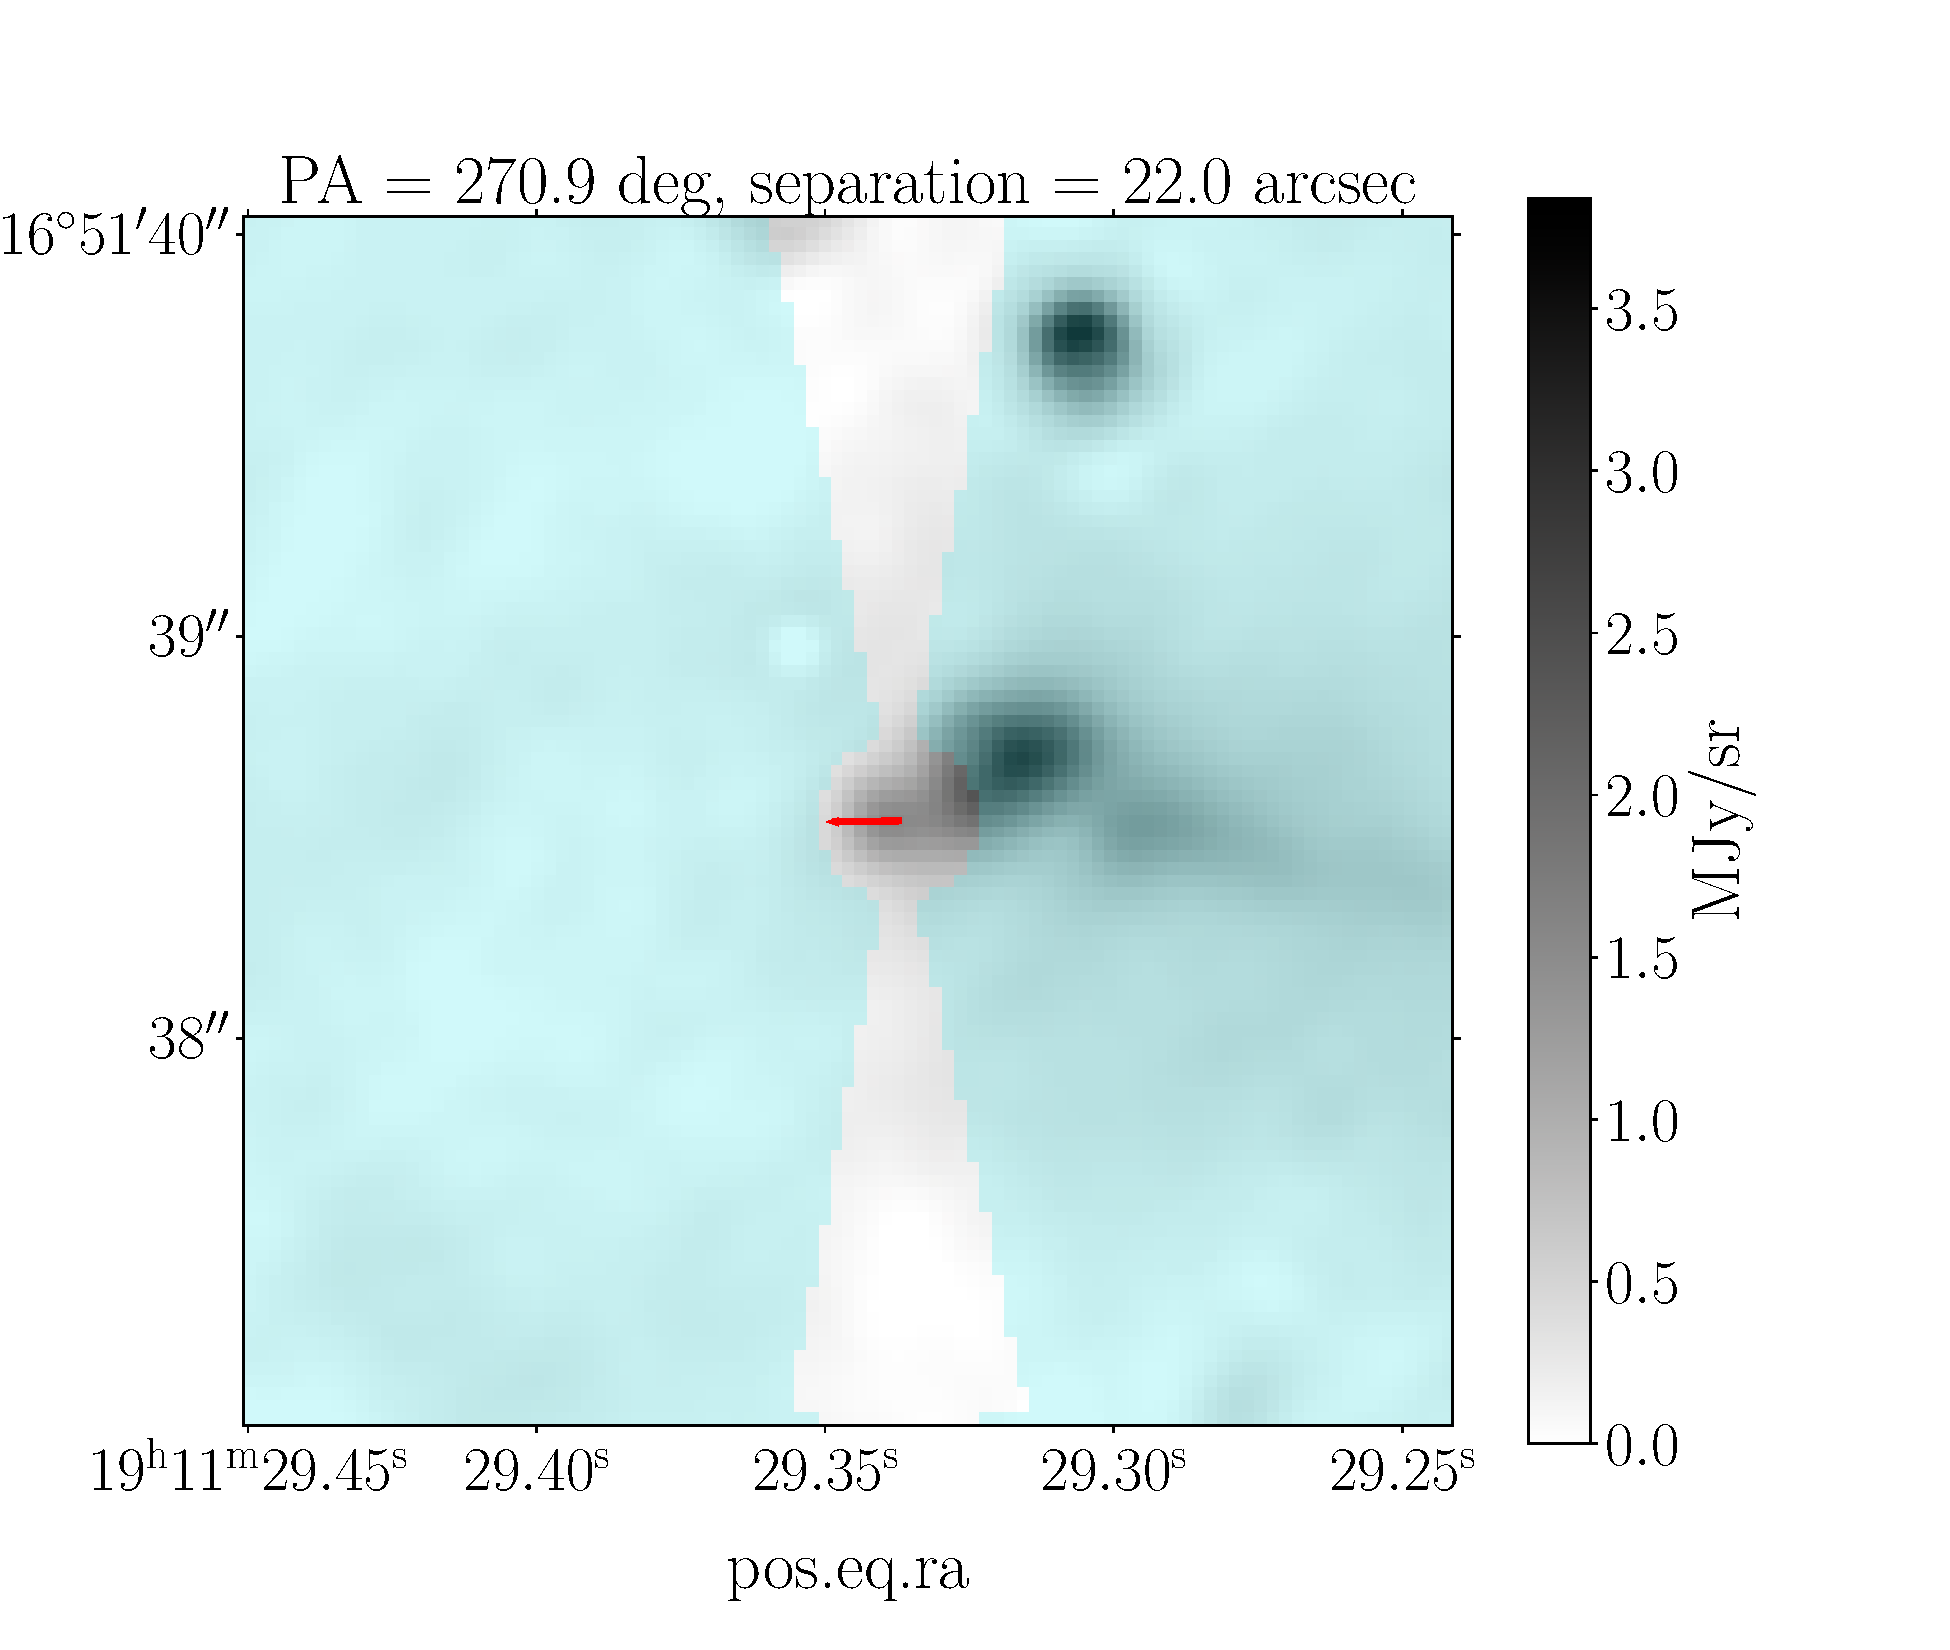
\includegraphics[width=0.8\textwidth]{Nuevas imagenes finales/r_0_.pdf}
  \caption{Example of the mask used to measure the radius of the
    neutral component of a globule. The mask is defined by the
    gray-scale pixels. To observe only neutral gas emission (PAHs),
    we used the combination of filters F150W, F210M, and F335M. The
    data are JWST observations.}
  \label{Medicion de r_0}
\end{figure}
  
\section[Observational errors]{Estimating uncertainties in the observational parameters}

For the uncertainties we consider that they arise from inhomogeneities
in the nebular brightness, unrelated to the globule or its shocked
shell, or from systematic effects due to the limitations of the model,
and not from photon noise. We therefore estimate these errors by
comparing different measurements, assuming they are independent.

\subsection{\boldmath Uncertainties in $r_\mathrm{shell}$ and $H_\mathrm{s}$}
\label{sec:error-shell}

For the radius and width of the shell, $r_\mathrm{shell}$ and
$H_\mathrm{s}$, respectively, we note that they follow a consistent
trend (see Figure \ref{fgi: Radios de la cascara}) when comparing the
measurements obtained with HST and JWST. For these measurements we
adopt the RMS uncertainty
\begin{equation}
    \sigma=\frac{\sqrt{\mathrm{Var}(x_\mathrm{J}-x_\mathrm{H})}}{\sqrt{2}},
\end{equation}
where $x_\mathrm{J}$ are the measurements from JWST using the ionized
gas composite, and $x_\mathrm{H}$ are the measurements from HST in
H$\alpha$ (see Appendix \ref{AP: errores r_s H_s}).

\begin{figure}[htb]
    \centering
    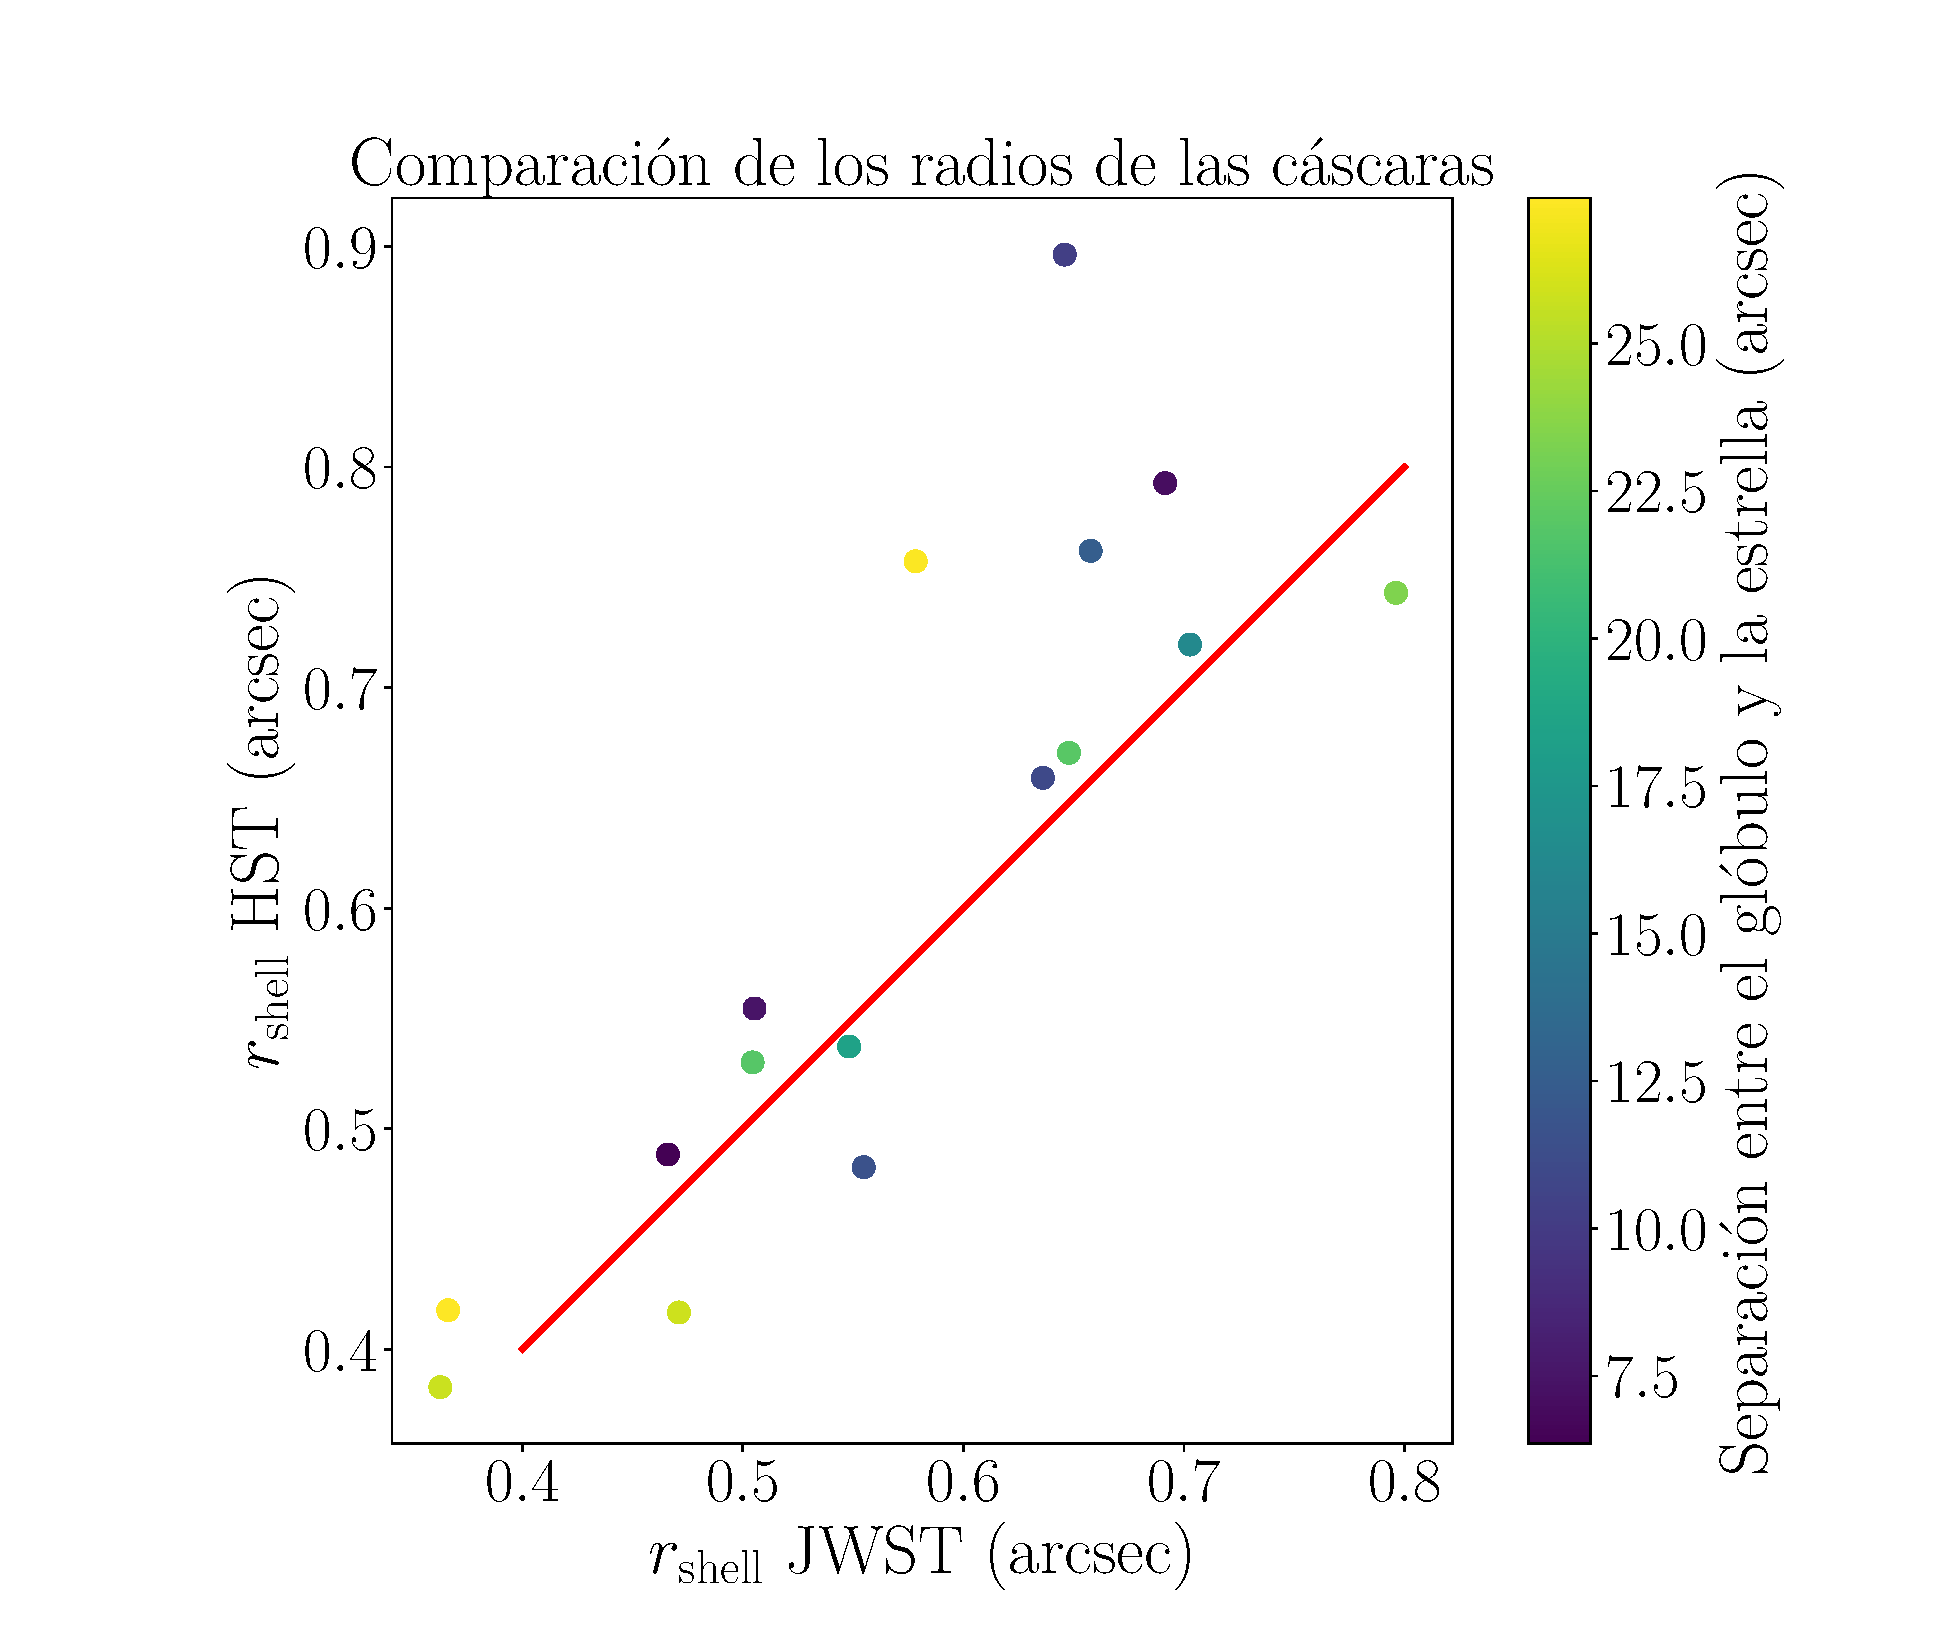
\includegraphics[width=\textwidth]{imagenes_corregidas/rshell.pdf}
    \caption{Comparison of shell radii (colored points) obtained from
      fits to both telescopes. Each point represents a globule for
      which a shell was detected in both instruments. The HST
      measurements are in the F656N filter, and the JWST measurements
      use the ionized-gas composite. The red line shows the 1:1
      relation, indicating that the two sets of measurements are very
      similar.}
    \label{fgi: Radios de la cascara}
\end{figure}

\subsection{\boldmath Uncertainty in $r_0$}

For the inner region we have one measurement of the neutral radius
using a JWST filter combination, and an approximate measurement with
HST, since the latter traces only ionized gas while the globule is
mainly neutral. Although there is not a strong correlation between the
two measurements (see Figure \ref{fig:Rcore dis}), their mean values
and standard deviations are very similar. We therefore adopt a single
radius for all globules: \SI{0.135}{\arcsecond}, the average of the
two mean values. As the uncertainty we adopt the standard deviation of
both measurements, which is the same, $\pm\SI{.03}{\arcsecond}$ (see
Figure \ref{fig:Rcore dis}).

\begin{figure}[htb]
    \centering
    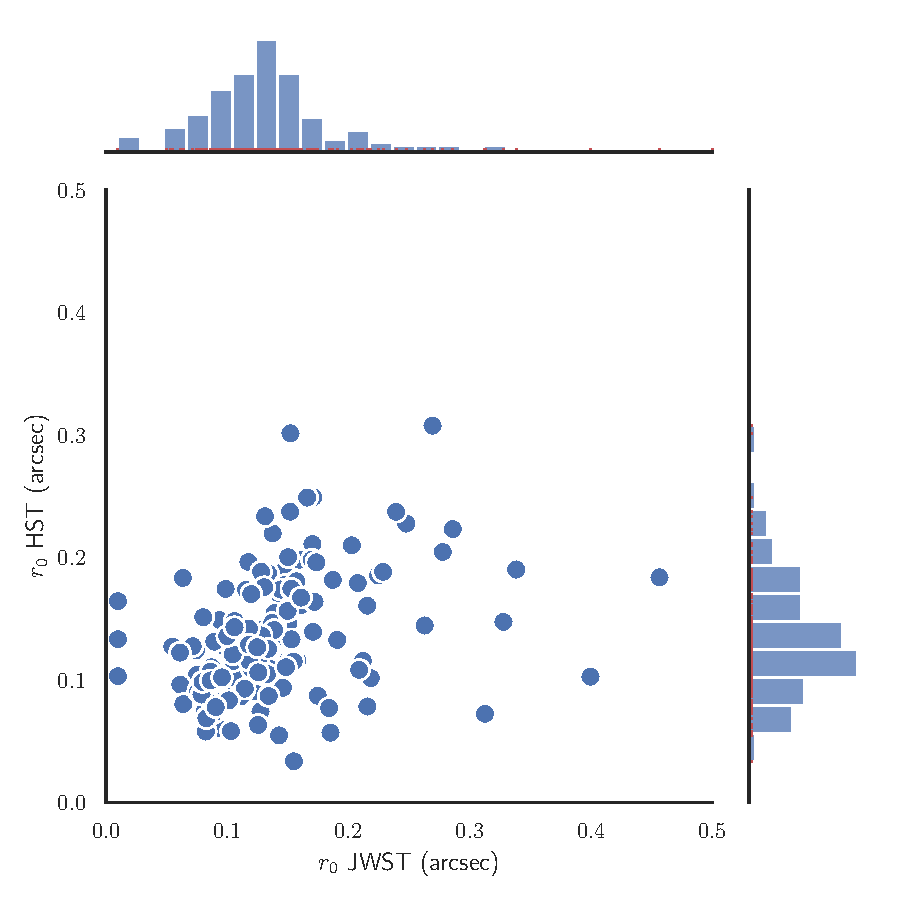
\includegraphics[width=0.8\textwidth]{imagenes_corregidas/r_0.pdf}
    \caption{Comparison of the radii of the neutral component measured
      with both instruments. The upper histogram shows the JWST
      measurements, with a mean value of \SI{0.15}{\arcsecond} and a
      standard deviation of \SI{0.03}{\arcsecond}. The right-hand
      histogram shows the HST measurements, with a mean of
      \SI{0.12}{\arcsecond} and a standard deviation of
      \SI{0.03}{\arcsecond}.}
    \label{fig:Rcore dis}
\end{figure}

\subsection{\boldmath Uncertainties in $B_\mathrm{s}$ and $B_0$}

For the surface brightnesses of the shocked shell and the globule,
$B_\mathrm{s}$ and $B_0$, respectively, we estimate the error as the
following standard deviation:
\begin{equation}
  \epsilon_{B}=\sqrt{\mathrm{Var}\Big(\overline{(y-\overline{y})^2},w*w_2\Big)}, 
\end{equation}
where $y$ is the brightness profile from the HST F656N filter minus
the fitted brightness profile, $w$ is the weight from the model
(equation \ref{eq: peso}), and $w_2$ is the fitted Gaussian
corresponding to the component in question. For the inner part $w_2$
is the first Gaussian centered at \SI{0}{\arcsecond}; for the shell
$w_2$ is the second Gaussian (see Figure \ref{ejemplo ajuste}).

With these uncertainty estimates we use the
\verb|uncertainties|\footnote{Documentation:
  \url{https://pythonhosted.org/uncertainties/}} package to compute
the error bars. This package calculates uncertainties using the theory
of linear error propagation, taking into account whether the data are
fully independent or correlated.

\section[\boldmath Estimating the ionized gas density from H$\alpha$
  surface brightness]{Estimating the ionized gas density from
  H$\alpha$ surface brightness}\label{Sec : estimacion de densidad}

To estimate the density of the ionized gas, we first use the
definition of the emission measure (EM):
\begin{equation}
\mathrm{EM}=\int_z n_\mathrm{i} n_\mathrm{e}\,dz,
\end{equation}
where $n_\mathrm{i}$ is the ion density, $n_\mathrm{e}$ the electron
density, and the integral is along the line of sight $(dz)$. If we
consider a fully ionized gas in which the electrons come only from
hydrogen, then $n_\mathrm{e}=n_\mathrm{i}=n$\footnote{There is in
  principle also a contribution from He, but we treat it as neutral
  because the star emits too few energetic photons to ionize He,
  compared to the ionizing photon rate for H
  \citep{Palmira:2020}.}. Thus $\mathrm{EM}=n^2 l$, where $n$ is the
RMS mean density and $l$ is the depth of the dense gas along the line
of sight.

\begin{figure}[htb]
    \centering
    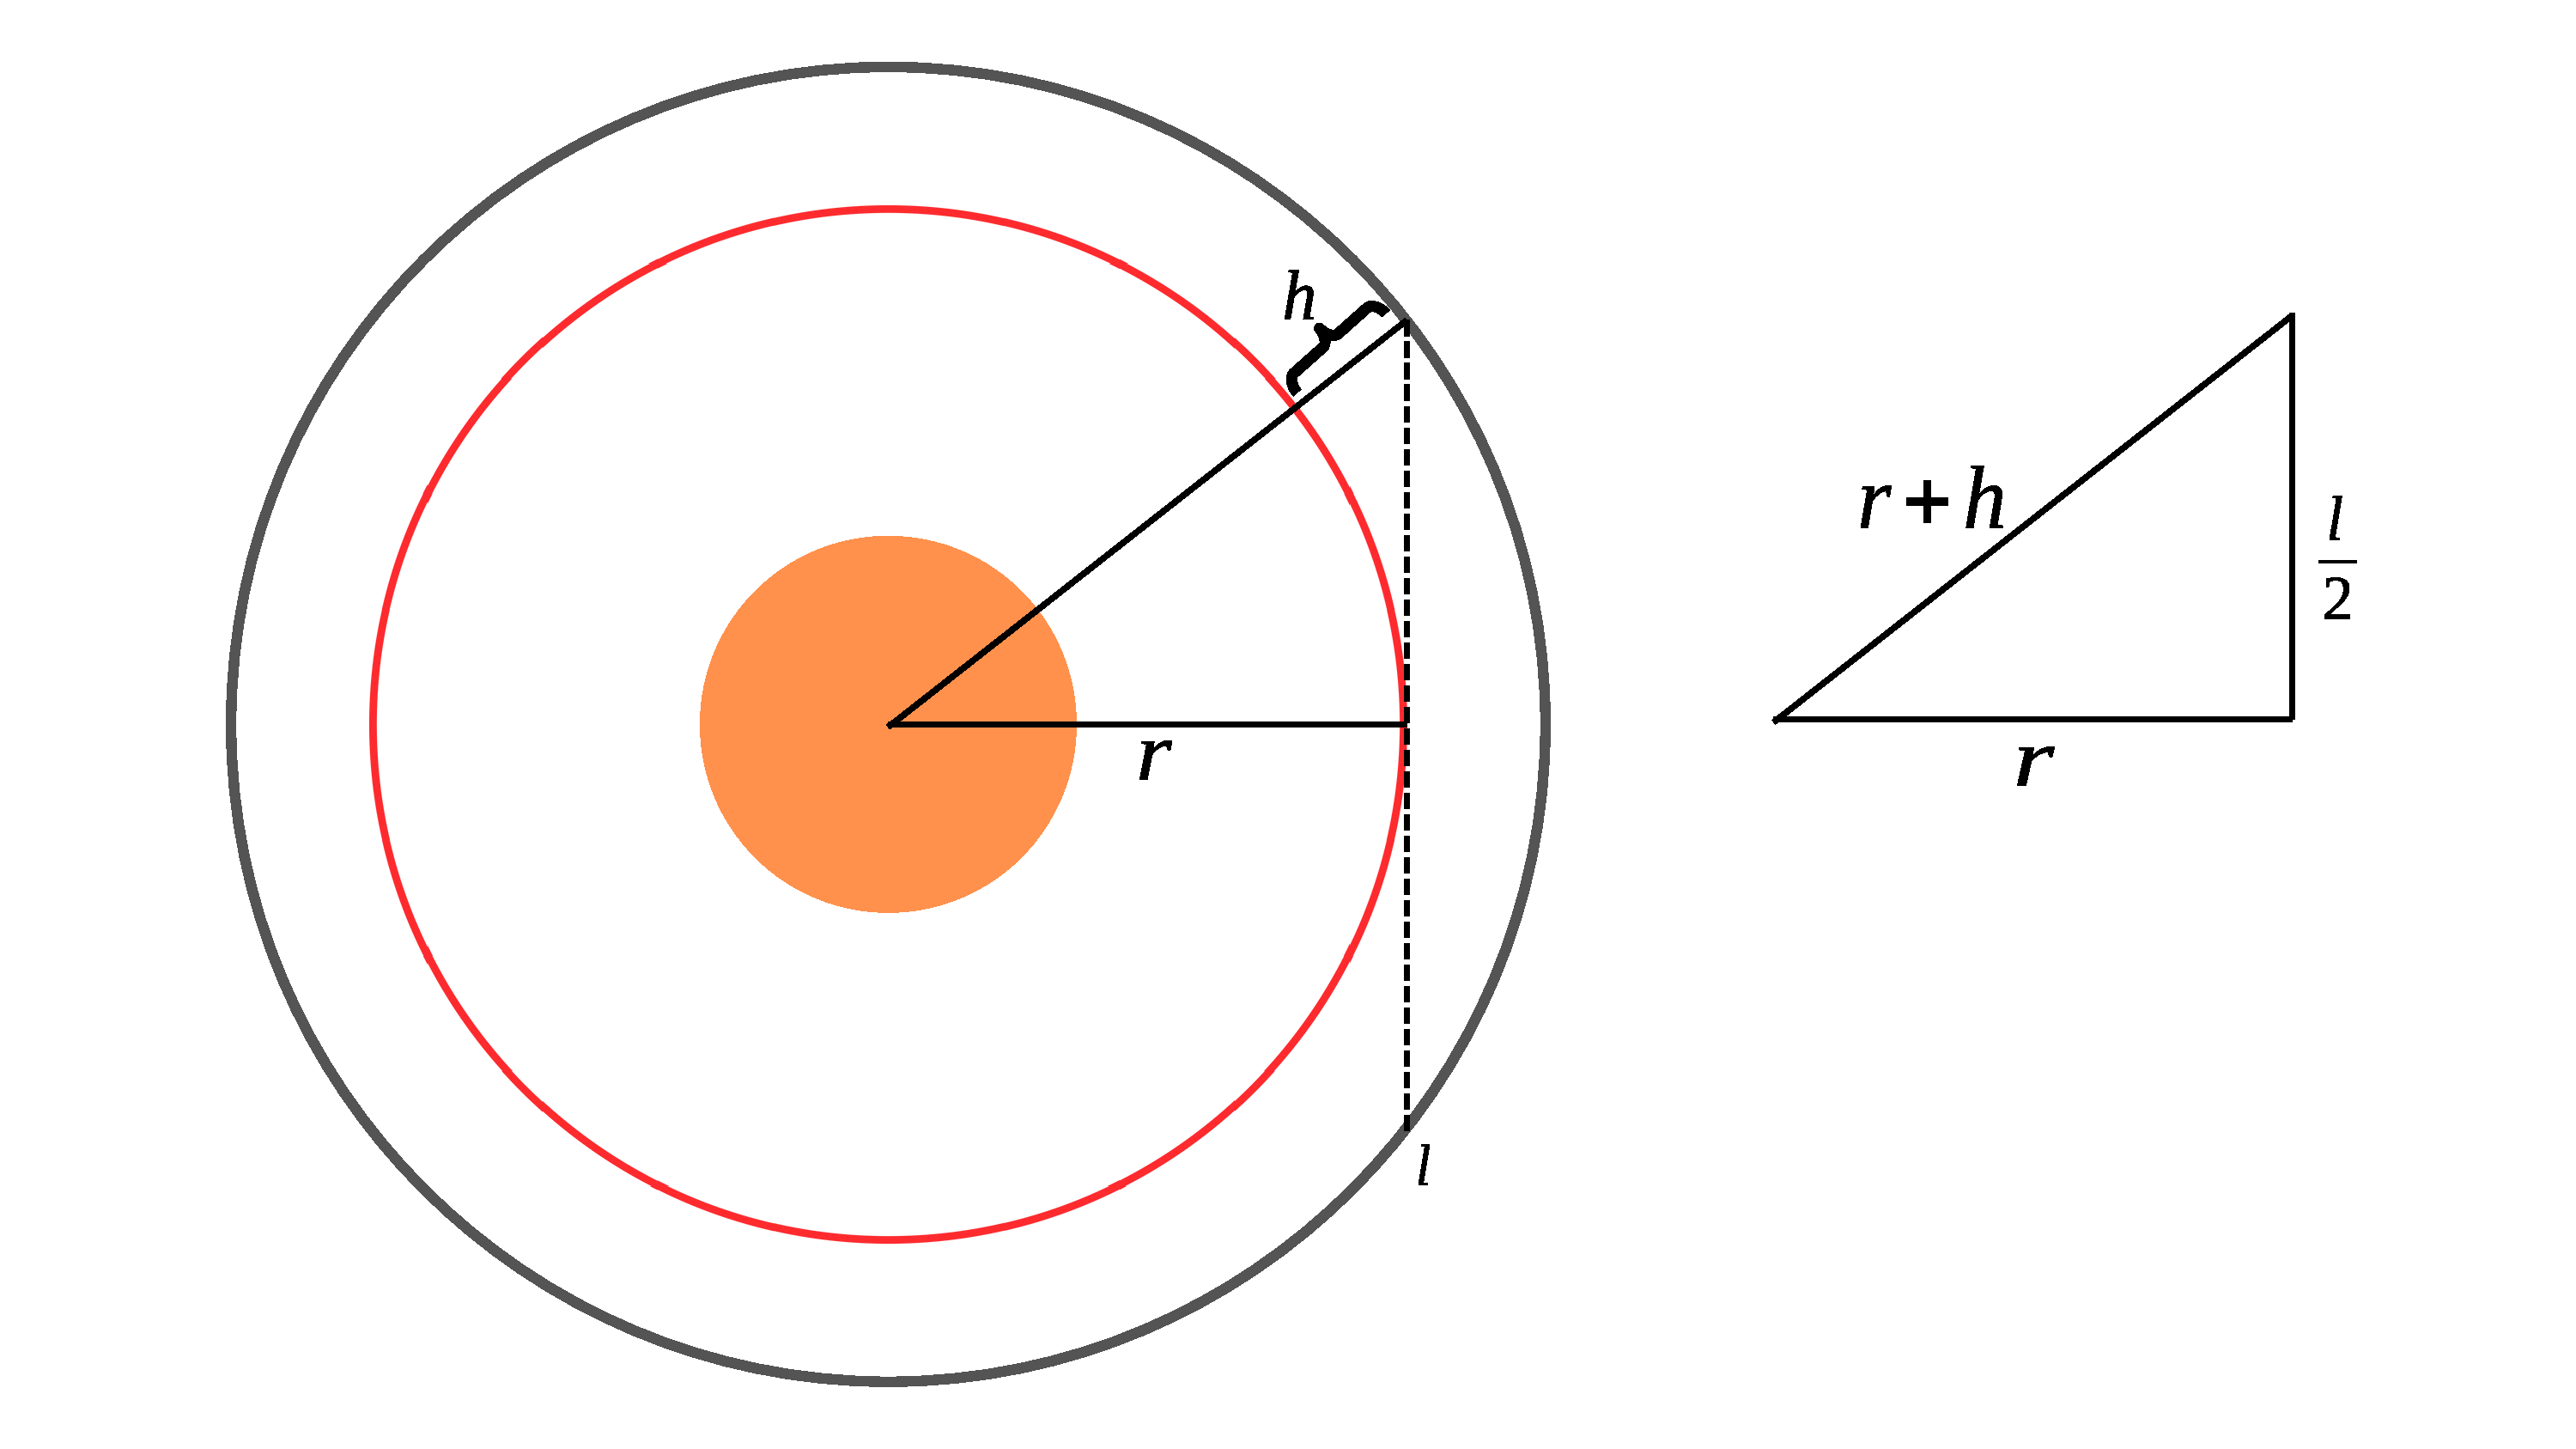
\includegraphics[width=\textwidth]{artesanales/ImgFi01-4.pdf}
    \caption{Schematic diagram showing a line of sight, with maximum
      path length $l$ (dashed line). Assuming spherical symmetry we
      obtain this configuration, where $h$ is the width of the shocked
      shell, $r$ is the radius from the globule center to the onset of
      the shocked photoevaporative flow, and $h<r$.}
    \label{fig:EM}
\end{figure}

Assuming a spherical shell of radius $r$, thickness $h$ with $h\ll r$,
and constant density, we obtain
\begin{equation}
  \mathrm{EM}=2\sqrt{2rh}\,n^2.
\end{equation}

From Figure \ref{fig:EM} we see that by geometry
$r^2+\Big(\frac{l}{2}\Big)^2=(r+h)^2=r^2+2rh+h^2\approx r^2+2rh$, hence
$l=2\sqrt{2rh}$. Therefore, using the EM we have
\begin{equation}
  n=\sqrt{\frac{\mathrm{EM}}{l}}=\sqrt{\frac{\mathrm{EM}}{2\sqrt{2rh}}}.
\end{equation}

In this work we apply this method to the detected shells, taking
$r=r_\mathrm{s}$ and $h=H_\mathrm{s}$.

\subsection{Using EM from the observations} \label{Subsec : EM}

In our HST observations the surface brightness is given in units of
\unit{counts.s^{-1}}. We use a conversion factor of 0.0137 to obtain
units of \unit{erg.s^{-1}.cm^{-2}.sr^{-1}} (see Appendix \ref{AP :
  conversion EM}). Dividing by the energy of an H$\alpha$ photon we
have
\begin{equation}
    B\frac{0.0137}{(h\nu)_{\mathrm{H}\alpha}}=\int \frac{f_{\mathrm{H}\alpha}\alpha_\mathrm{B} n_\mathrm{e} n_\mathrm{p}}{4\pi}\,dz,
\end{equation}
where $B$ is the observed surface brightness,
$(h\nu)_{\mathrm{H}\alpha}$ is the photon energy of H$\alpha$,
$f_{\mathrm{H}\alpha}$ is the fraction of all recombinations to levels
$n\geq 2$ that result in H$\alpha$ emission, $\alpha_\mathrm{B}$ is the
case B recombination coefficient, $n_\mathrm{e}$ is the electron
density, and $n_\mathrm{p}$ the ion density. The integral on the right
is along the line of sight.

If we take both $f_\mathrm{H\alpha}$ and the recombination coefficient
as constants, then
\begin{equation}
    B\frac{0.0137}{(h\nu)_{\mathrm{H}\alpha}}=\frac{f_{\mathrm{H}\alpha}\alpha_\mathrm{B}}{4\pi}\int n_\mathrm{e} n_\mathrm{p}\,dz,
\end{equation}
where the integral is the EM. Assuming
$f_\mathrm{H\alpha}=0.5$ and
$\alpha_\mathrm{B}=\SI{2.3e-13}{cm^{3}.s^{-1}}$, we obtain
$f_{\mathrm{H}\alpha}\alpha_\mathrm{B}=\SI{1.17e-13}{cm^3.s^{-1}}$. The
EM can then be derived directly from the observations as
\begin{equation}
    \mathrm{EM} = B\frac{0.0137}{(h\nu)_{\mathrm{H}\alpha}}\frac{4\pi}{\SI{1.17e-13}{cm^3.s^{-1}}},
\end{equation}
which yields EM in units of \unit{cm^{-5}} (cgs).

It is important to note that in deriving the density from EM and $l$,
we are assuming that $l$ is perpendicular to the symmetry axis of the
model.

In Figure \ref{fig:dens_angl} we show that the maximum density $n_1$
lies along the symmetry axis and decreases with angle as
$\cos^{1/2} i$ \citep{Tarango:2018}.

\begin{figure}[htb]
  \centering
  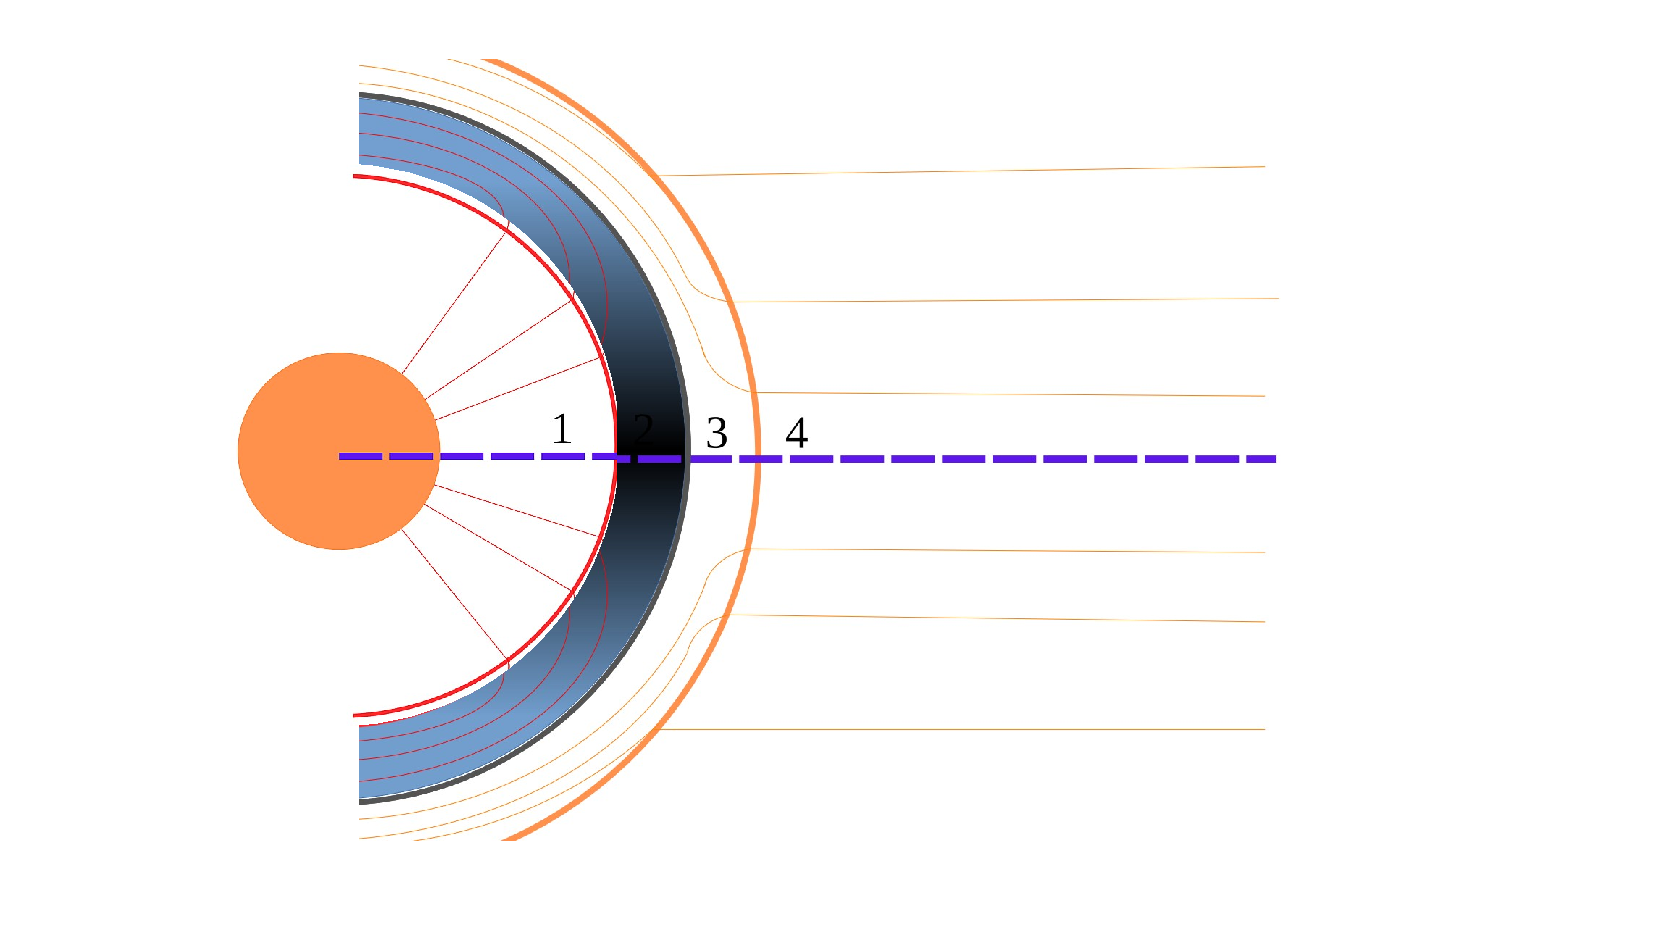
\includegraphics[width=\textwidth]{Nuevas imagenes finales/densi_angle.pdf}
  \caption{Along the symmetry axis the shocked shell has a maximum
    density $n_1$ (darker color), which decreases with increasing
    angle from the axis (lighter color).}
  \label{fig:dens_angl}
\end{figure}
  
\section{Good fits}\label{Good results}

For 16 globules we obtained good fits, since the measurements matched
both the globules and the shocked shells that could be visually
identified in the images. From these fits we now know $r_0$,
$r_\mathrm{shell}$, and $H_\mathrm{s}$. In addition, we have measured
the brightness both in the inner region and in the shocked shell, so
we can extract further information. In Section \ref{Sec : estimacion
  de densidad} we showed how to estimate the density in the shocked
shell from its brightness, which then allows us to determine the shell
pressure,
\begin{equation}
    P_\mathrm{shell}=\rho c_\mathrm{s}^2.
\end{equation}
This pressure can be compared with the RAM pressure of the stellar
wind. We can also estimate the internal pressure of the globule and
compare it directly with the model.

These well-fit globules span a wide range of separations from the
star, so they provide a representative view of the nebula and the
globules in general. Figure \ref{Goog G} shows examples of good fits,
where the globule and its shocked shell are clearly identifiable.

\begin{figure}[htb]
    \centering
    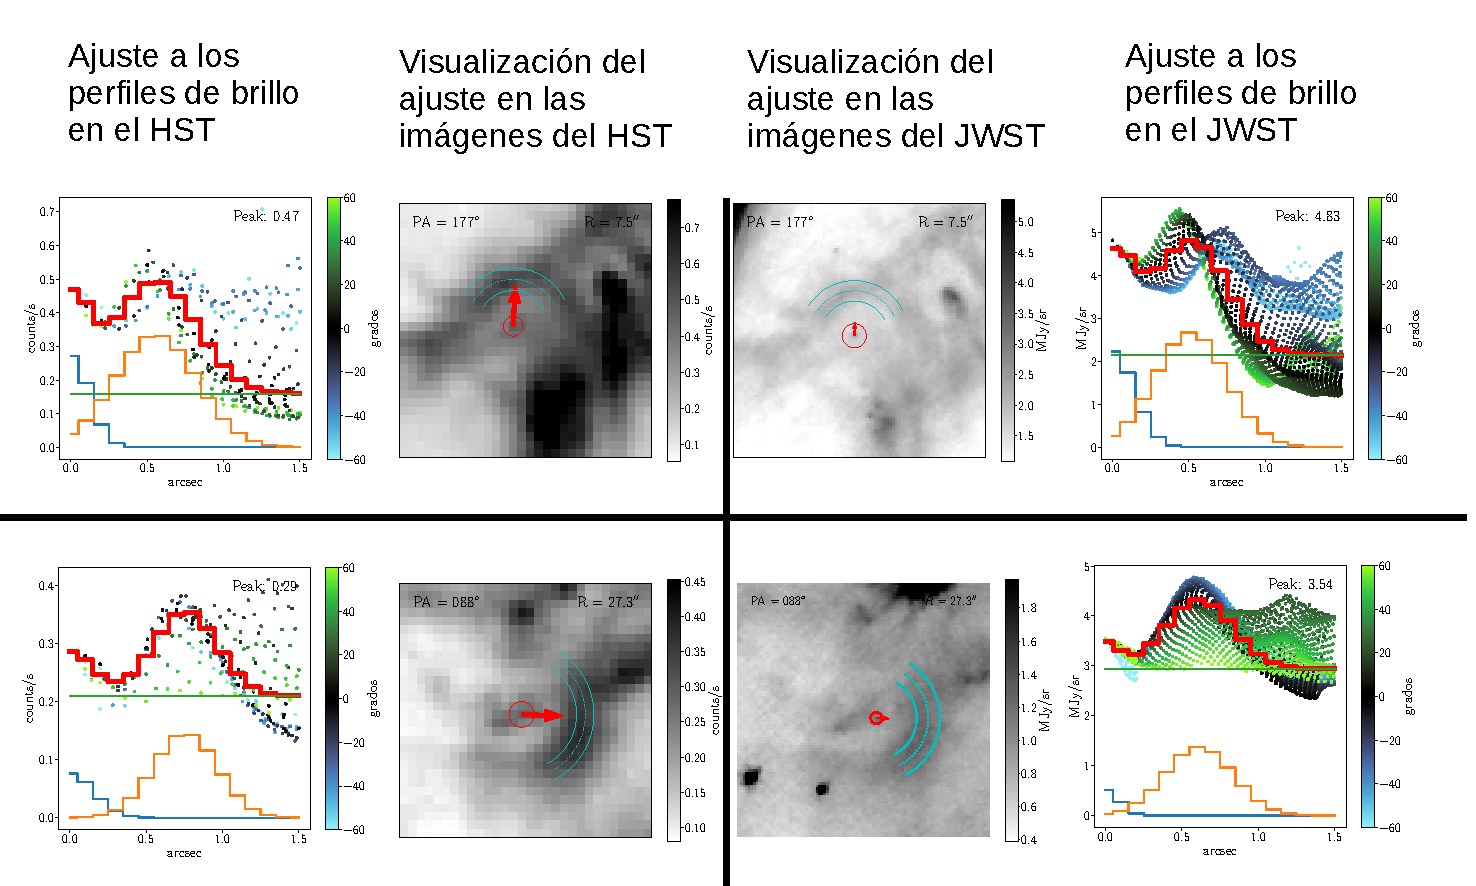
\includegraphics[width=\textwidth]{imagenes_corregidas/buenos_aj.pdf}
    \caption{Examples of good fits. Left panels: brightness-profile
      fits (left subpanel) and the corresponding HST image (right
      subpanel). Right panels: JWST data. The fits shown are for the
      ionized-gas composite (Figure \ref{fig:filters WR124}), but the
      visualizations are in the F090W filter, since its morphology is
      very similar to the HST images.}
    \label{Goog G}
\end{figure}

\section{Recovered fits}

By fitting the brightness profiles from two telescopes with different
resolutions, we obtained improved results. In some globules, even
though their shocked shells were visible by eye, our algorithm failed
to detect them in one of the two images.

Figure \ref{Recuperados Globulos} shows examples where a possible
shell can be seen visually, but the brightness-profile fit fails to
detect it in one telescope (top left and bottom right panels), due to
scatter in the data points or to too few points, as in the HST data.
Another reason for poor detection was that the shell often had very
low brightness.

In this way we increased the sample size beyond the initial set,
resulting in a final sample of 30 globules for which we know the
globule size, the shocked shell radius and width, and the surface
brightness at the globule center and in the shocked shell\footnote{All
  of these fits are shown in Appendix \ref{App : ajustes}}. With these
measurements we can compare the pressure of the shocked shells with
the RAM pressure of the stellar wind. Thus in Chapter \ref{Ch :
  balance de presiones} we will compare our model directly with the
observations.

\begin{figure}[htb]
    \centering
    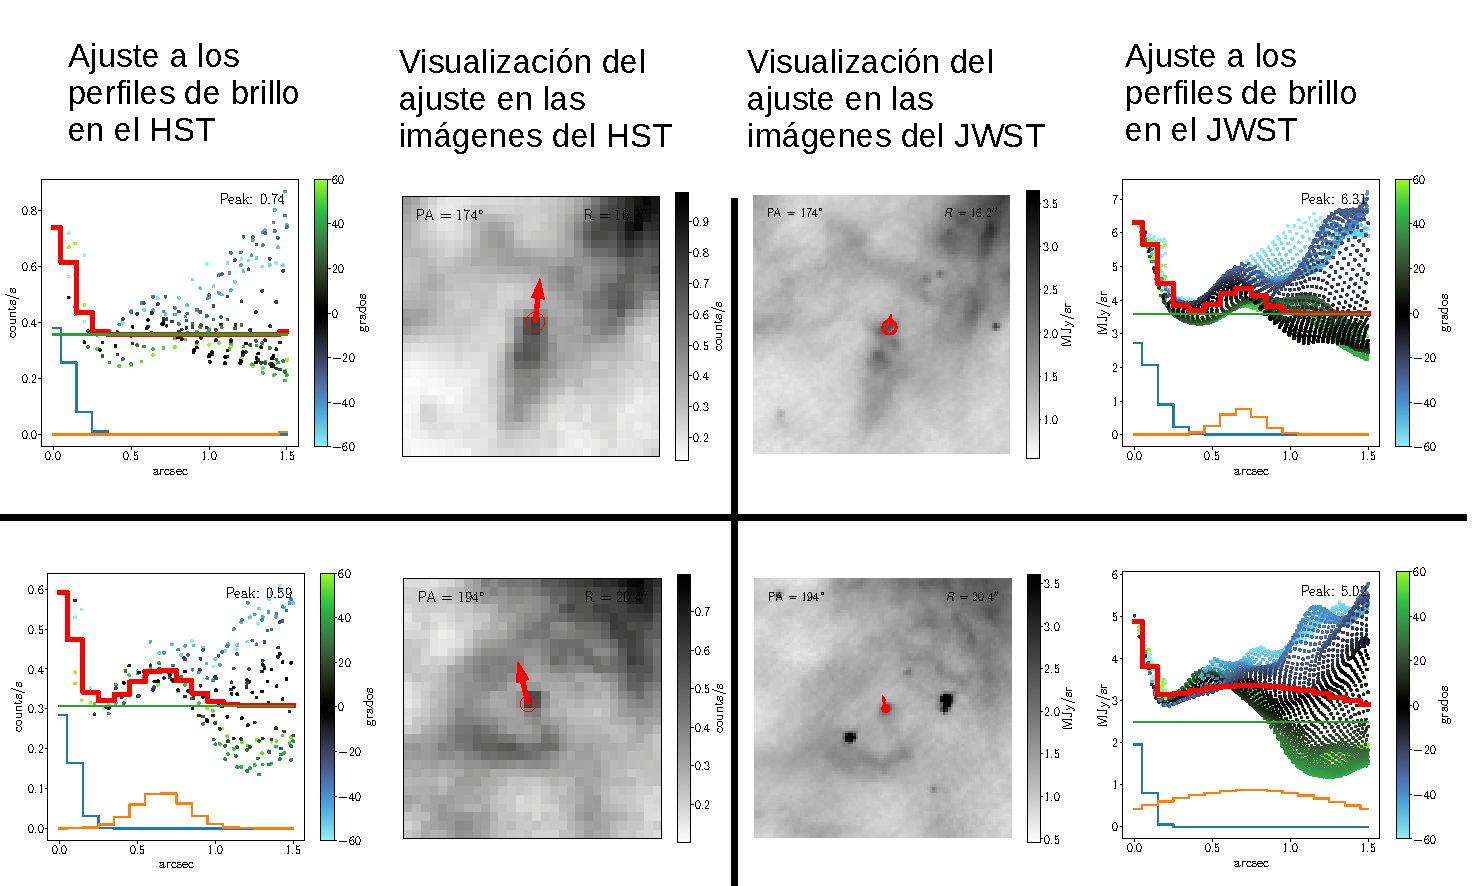
\includegraphics[width=\textwidth]{imagenes_corregidas/recuperados_aj.pdf}
    \caption{Examples of recovered fits. In these images the shell is
      visible by eye, but the brightness-profile fitting fails to
      detect the shocked shell in one telescope (top left and bottom
      right panels), due to scatter in the points.}
    \label{Recuperados Globulos}
\end{figure}

\section{Discarded globules}\label{Bad globules}

Despite having a substantial number of globules suitable for applying
the model, not all could be used. Some had poor fits due to the large
scale structure of the nebula, contamination by background stars, or
the diffraction spikes of bright stars. In such cases the neutral
region or the shocked shell could not be reliably detected, or their
sizes were incorrectly determined. Figure \ref{Bad Globules} shows
examples of globules whose shocked shells could not be reliably
measured.

\begin{figure}[htb]
    \centering
    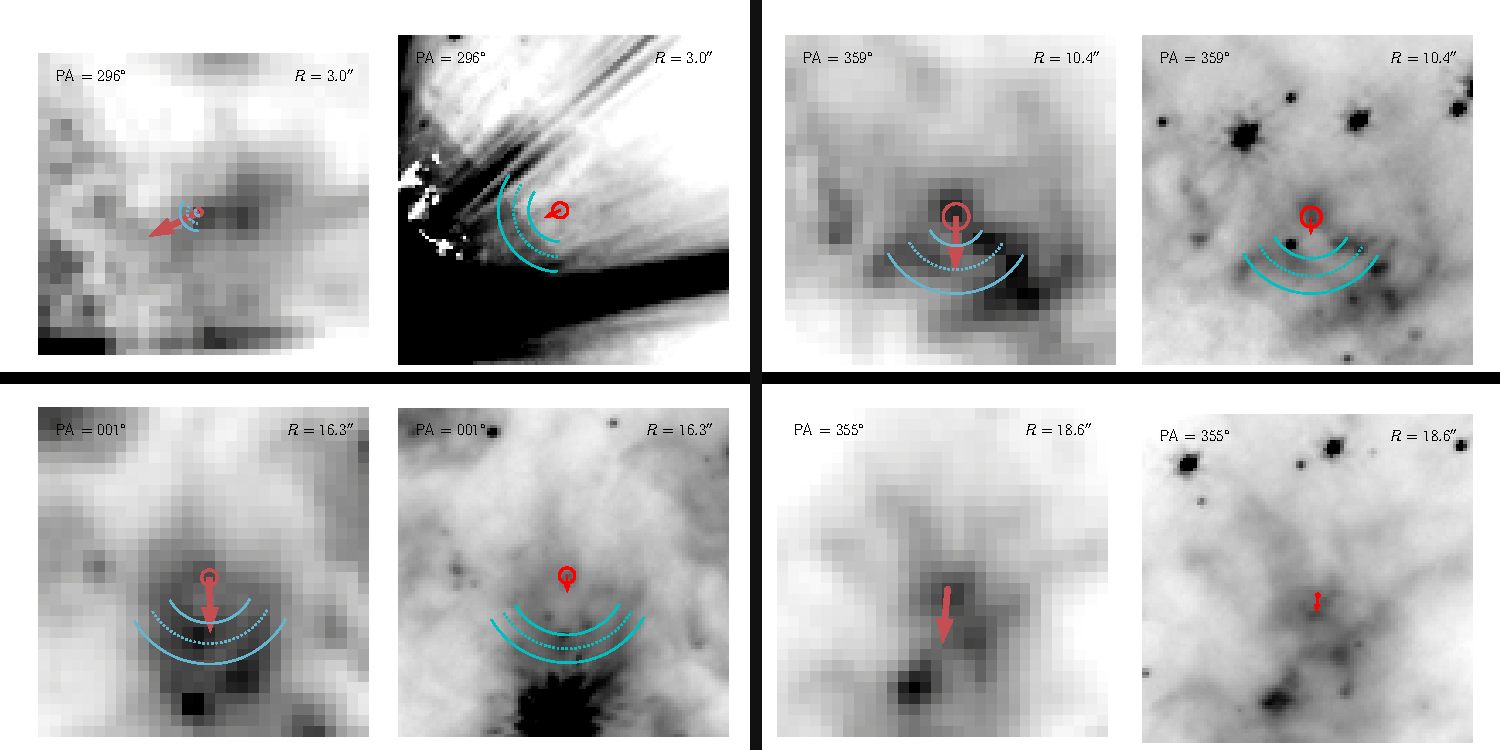
\includegraphics[width=\textwidth]{Nuevas imagenes finales/Malos_ajustes_final.pdf}
    \caption{Examples of discarded globules. Left: HST images; right:
      JWST F090W filter. The first globule is discarded because it is
      affected by telescope diffraction and by the large-scale nebular
      structure, likely due to its proximity to the central star. In
      the other examples, nearby sources compromise the measurements
      of possible shocked shells.}
    \label{Bad Globules}
\end{figure}

Table \ref{tab:mean} lists the mean values of the different measured
quantities, taking the scatter among the globules as the uncertainty.
The mean separation between the globules and the star is
$14.96\pm\SI{7.1}{\arcsecond}$. The globule radius and shell width are
both smaller than the shell radius. The density is typically of order
\SI{e3}{cm^{-3}}, while the shell pressures are of order
\SI{e-9}{dyn.cm^{-2}}. Finally, $n_\mathrm{i,0}$ is the ionized-gas
density at the ionization front of the globules, assuming ionization
equilibrium.

\begin{table}[htb]
  \centering
  \begin{tabular}{c c}
    \toprule
    \multicolumn{2}{c}{Results of the good fits} \\ \midrule
    Separation & 14.96$\pm$\SI{7.1}{\arcsecond}\\
    Globule radius $r_0$ & 0.135$\pm$\SI{0.03}{\arcsecond} \\
    Shell radius $r_\mathrm{shell}$& 0.62$\pm$\SI{0.13}{\arcsecond}\\
    Shell width $H_\mathrm{s}$ & 0.24$\pm$\SI{0.1}{\arcsecond}\\
    $n_\mathrm{shell}$ & 1.37$\pm$\SI{.05e3}{cm^{-3}}\\
    $n_\mathrm{i,0}$ & 5.01$\pm$\SI{.55e3}{cm^{-3}}\\
    $P_\mathrm{shell}$ & 1.89$\pm$\SI{.06e-9}{dyn.cm^{-2}}  \\
    $r_\mathrm{shell}/r_0$ & 4.4$\pm$1 \\\bottomrule
  \end{tabular}
  \caption{Mean values of the results obtained from the fits. The
    uncertainties are the scatter among different globules.}
  \label{tab:mean}
\end{table}
  
\chapter{Pressure balance in the shells}\label{Ch : balance de presiones}

In this chapter we use the measurements obtained from the various
observations of the globules in the M1-67 nebula. In this way we can
investigate the pressure balance between the photoevaporative flow
from the globules and the stellar-wind pressure, and finally compare
directly with the stationary hydrodynamic model that we propose. If
the observations are consistent with our model, then we will gain a
better understanding of the spatial distribution of the globules in
the M1-67 nebula.

We identified 168 globules in the nebula, distributed at distances of
3--\SI{35}{\arcsecond} (7--\SI{92e-2}{pc}) from the central star.
These globules appear either in groups or in isolation, as shown in
Figure \ref{fig:dis_nudos}.

Although we could not obtain good fits for all the globules, we still
have a very useful sample, as they are distributed over a wide range
of distances from the star and show a wide variety in the measured
parameters.

\section{Internal pressure balance}\label{Sec : comparacion-modelo}

We now compare directly with the model (see Figure
\ref{fig:grafica_C2}). Specifically, we compare the ratio of the
pressure in the shocked shell of the globule to that at the globule
surface against the ratio of the shell radius to the globule radius.
Recall that Figure \ref{fig:grafica_C2} shows $P/P_0$ as a function of
$r/r_0$.

Since we are considering a stationary model, the pressure in the
shocked shell—where we consider only the thermal pressure—must equal
the total pressure just before $r_\mathrm{shell}$. In Chapter
\ref{Chapter : Modelo} we showed that the model predicts $f$ as a
function of $r/r_0$, giving the pressure of the photoevaporative flow
just before the shock, normalized by the pressure at the globule base,
as a function of radius.

The ratio of the radii is straightforward, since we measured these
parameters directly for each globule. Because we have also measured
the brightness and sizes of both the globule and the shocked shell, we
can calculate their respective densities.

For the ratio of the pressures at the globule base and in the shocked
shell, recall from Section \ref{Subsec : EM} that
$\mathrm{B}\propto \mathrm{EM}=n^2l$, hence
\begin{equation}
\frac{\mathrm{B_\mathrm{s}}}{\mathrm{B_0}}=\frac{n_\mathrm{s}^2l_\mathrm{s}}{n_0^2l_0},
\end{equation}
where $\mathrm{B_\mathrm{s}}, \; n_\mathrm{s}$, and $l_\mathrm{s}$ are
the brightness, density, and line-of-sight depth (perpendicular to the
symmetry axis) for the shell (see Figure \ref{fig:EM}), and
$\mathrm{B_0}, \; n_0$, and $l_0$ are the corresponding quantities for
the inner region. For the observations we have
$f_\mathrm{obs} =
\frac{P_\mathrm{shell}}{P_0}=\frac{\rho_\mathrm{shell}}{2\rho_0}
\Rightarrow \frac{\rho_\mathrm{shell}}{\rho_0}=2f_\mathrm{obs}$, so
\begin{equation}
\frac{\mathrm{B_\mathrm{s}}}{\mathrm{B_0}}=4f_\mathrm{obs}^2\frac{l_\mathrm{s}}{l_0}
\;\;\Rightarrow\;\; f_\mathrm{obs}= \frac{1}{2}\Big(\frac{\mathrm{B_\mathrm{s}}/\mathrm{B_0}}{l_\mathrm{s}/l_0}\Big)^{1/2}.
\end{equation}
In this way we can compare directly with the model. Appendix
\ref{App:brillos} gives details of the brightness corrections.

Because the globules are very small, we take
$r_0\approx l_0$\footnote{From Section \ref{Subsec : EM} we have
  $l_0=2\sqrt{2hr}=2\sqrt{2h/r_0}r_0=0.98 r_0\approx r_0$, using
  $h/r_0\approx0.12$ (see Appendix \ref{App : tasa de
    fotoionizacion}).}. Thus the comparison with the model follows
directly from the observations.

\begin{figure}[htb]
    \centering
    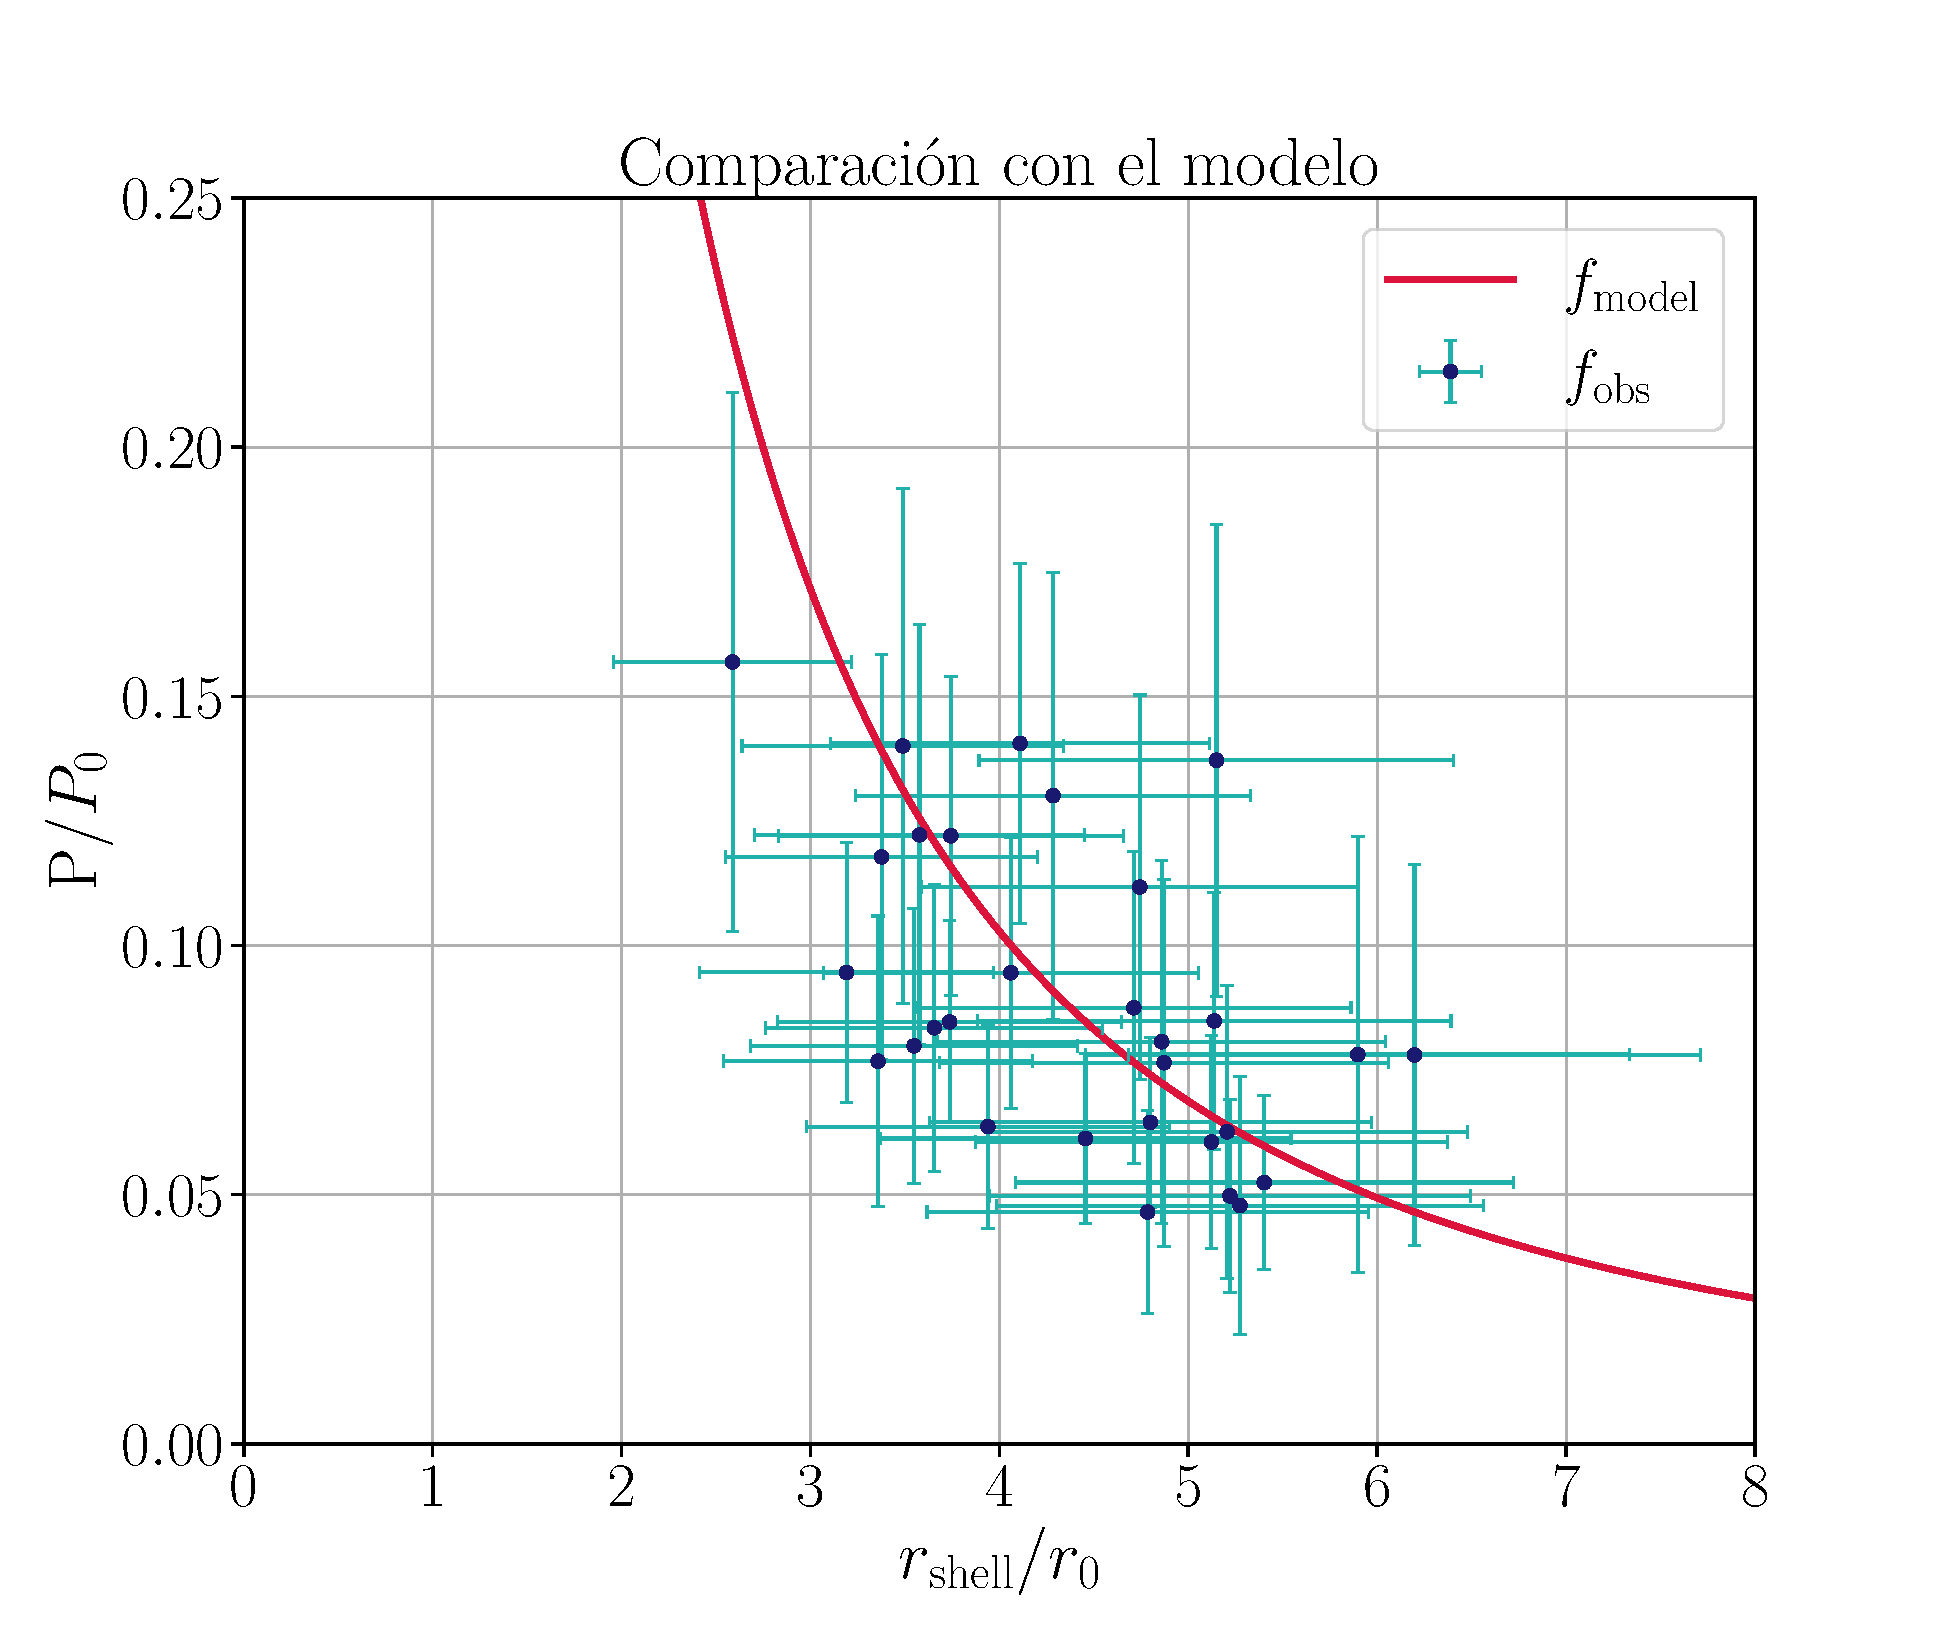
\includegraphics[width=\textwidth]{imagenes_corregidas/Model.pdf}
    \caption{$f_\mathrm{model}$ is the theoretical curve obtained from
      the proposed model, while $f_\mathrm{obs}$ is the ratio between
      the pressure in the shocked shell and the pressure at the
      globule surface from the observations.}
    \label{Resultados_modelo}
\end{figure}

Figure \ref{Resultados_modelo} shows that the observational results
closely match the predictions of the proposed model. The observations
fall mostly in the range $r_\mathrm{shell}/r_0=3$--6 (the ratio of
shell radius to globule radius), while the pressure ratios fall in the
range $f_\mathrm{obs}=0.05$--0.15. The observed data also show a
scattered anti-correlation.

Since the model has no free parameters and the observational results
agree well with its predictions, we conclude that the model provides a
valid explanation of the interaction between the supersonic flows. In
Figure \ref{Resultados_modelo} we see that the observational
measurements of $f_\mathrm{obs}$ are consistent with the model
predictions $f_\mathrm{model}=P/P_0$ (equation \ref{eq : 1}), within
the error bars.

\section{External pressure balance}\label{Sec:proyeccion}

In Figure \ref{graf_presion} we plot the shell pressure of the globules
as a function of their projected separation from the star. The purple
points show the shell pressures, while the red line shows the RAM
pressure of the stellar wind. We see that the globule shell pressures
fall below the stellar-wind RAM pressure if the projected separation
is taken as the true separation. In our model, however, the shell
pressure must be in equilibrium with the RAM pressure, so the observed
separation is likely only a projected one.

\begin{figure}[htb]
    \centering
    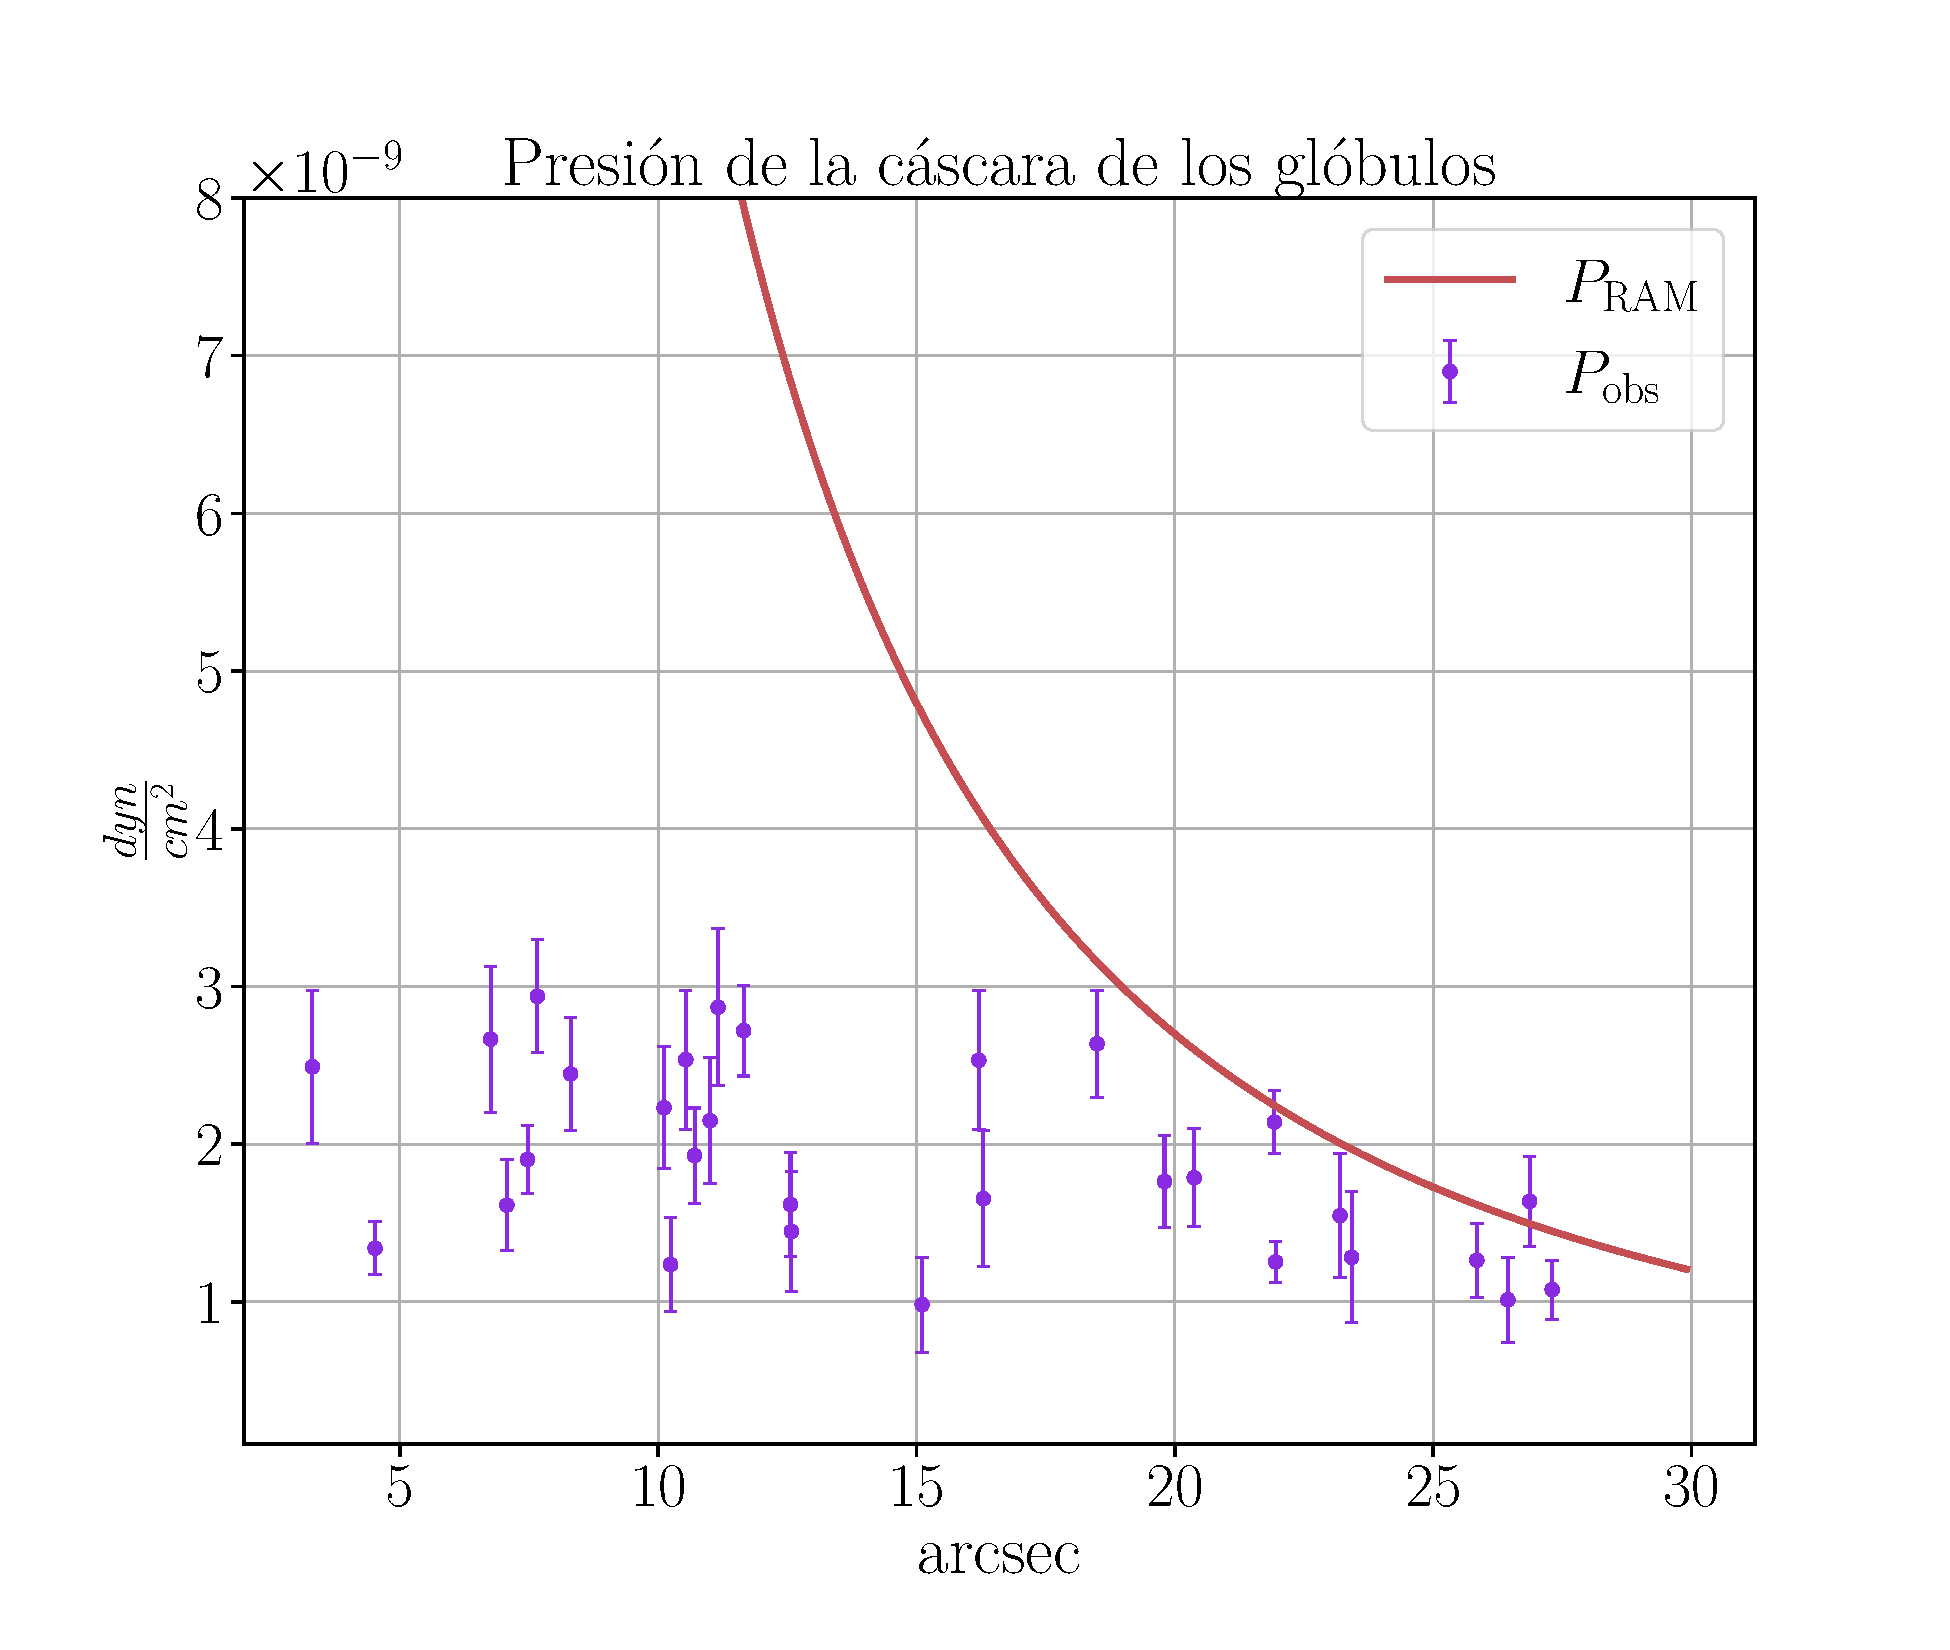
\includegraphics[width=\textwidth]{imagenes_corregidas/S_R.pdf}
    \caption{Shell pressures of the globules (purple circles) compared
      with the stellar-wind RAM pressure (red line), assuming the
      projected separation equals the true separation.}
    \label{graf_presion}
\end{figure}

If the globule is projected by an angle $i$ (see Figure
\ref{Ang proyeccion}), then
\begin{equation}
R\cos i=R_\mathrm{p},
\end{equation}\label{eq:sep_real}
where $R$ is the true separation from the star, $i$ the inclination
angle, and $R_\mathrm{p}$ the projected distance that we observe. Note
that the shell pressure equals the stellar-wind RAM pressure only
along the symmetry axis, and as seen in Section \ref{Subsec : EM}, off
the axis the shell pressure decreases by a factor of $\cos^{1/2}i$
\citep{Tarango:2018}. Thus, including this inclination factor, we have
\begin{equation}
    P_\mathrm{shell}(i)=\rho\cos^{1/2}(i) c_\mathrm{s}^2 \;\;\Rightarrow\;\;
    P_\mathrm{shell}(i)\cos^{-1/2}(i)=\rho c_\mathrm{s}^2,
\end{equation}
and therefore
\begin{equation}
P_\mathrm{shell}(i)\cos^{-1/2}(i)=\frac{\dot{M}v_\infty}{4\pi R^2}
\;\;\Rightarrow\;\;
P_\mathrm{shell}(i)=\frac{\dot{M}v_\infty}{4\pi R_\mathrm{p}^2}\cos^{5/2}i.
\end{equation}\label{eq:cos 5_2}

\begin{figure}[htb]
    \centering
    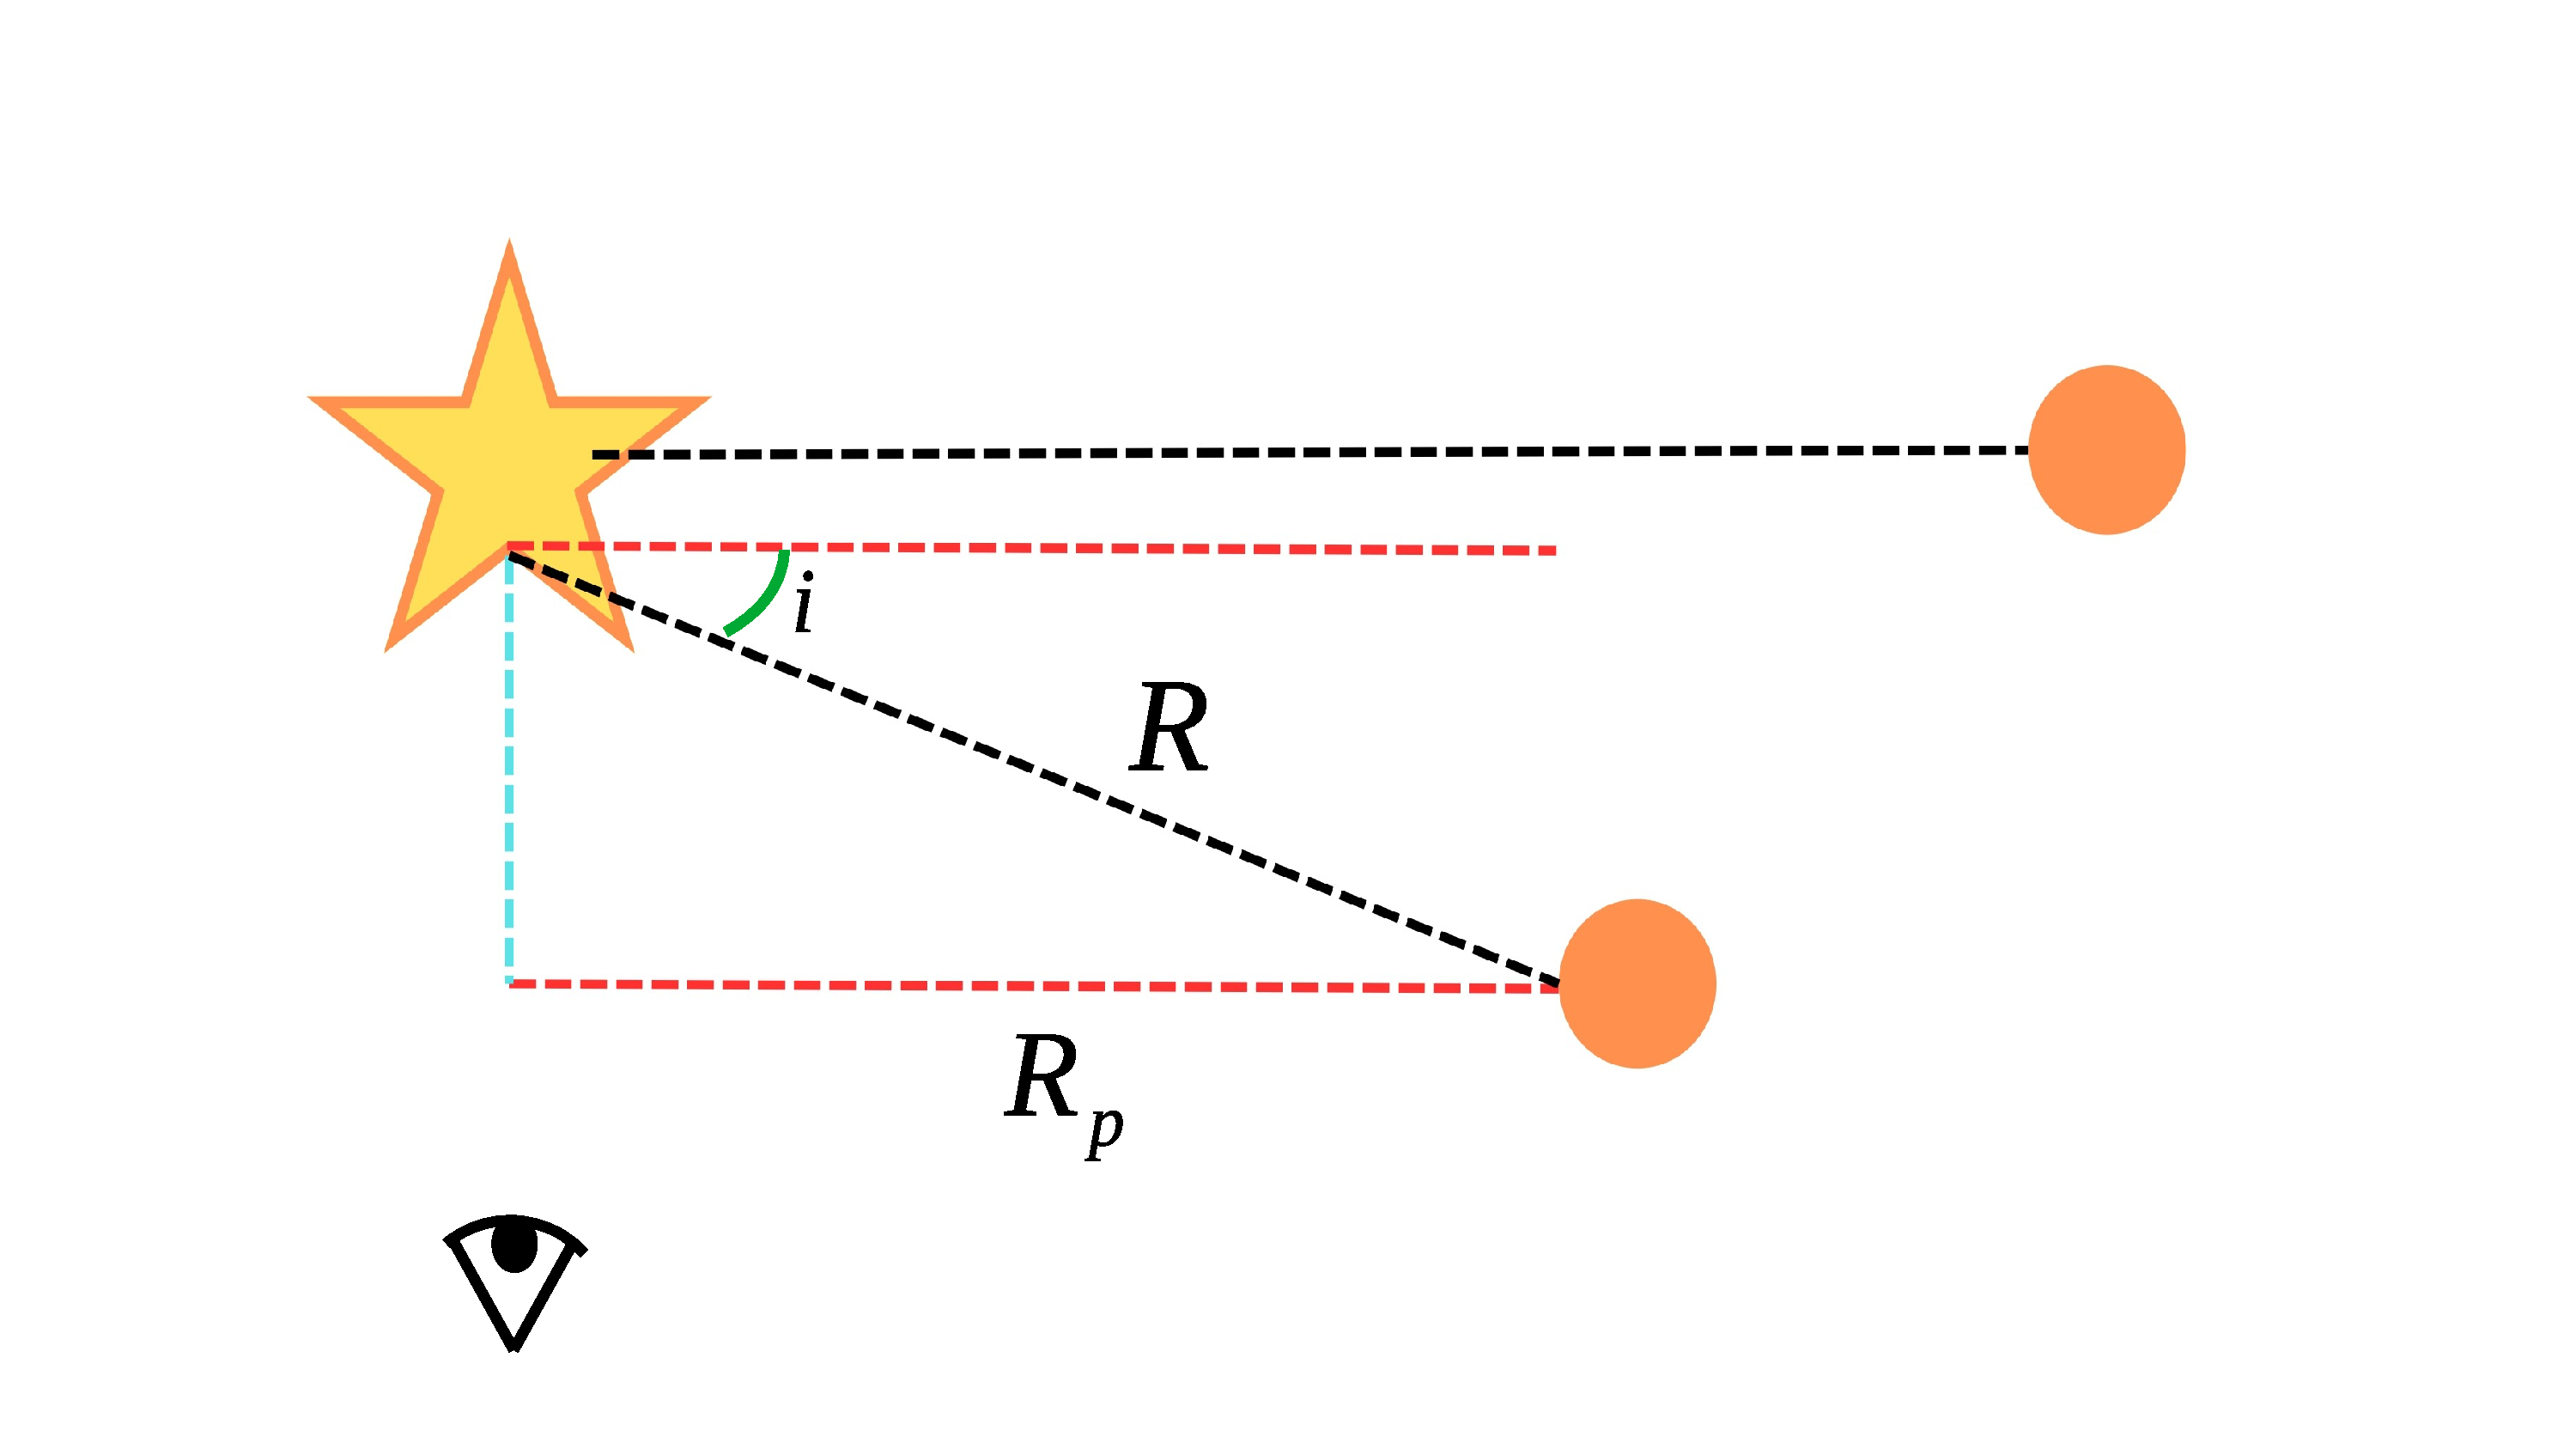
\includegraphics[width=\textwidth]{artesanales/ImgFi01-6.pdf}
    \caption{Illustration of how some globules are affected by an
      inclination angle relative to our line of sight. For the lower
      globule the true distance to the star is $R$, while we observe
      $R_\mathrm{p}$, the projected distance at angle $i$. The upper
      globule is not affected by projection.}
    \label{Ang proyeccion}
\end{figure}

With this equation we can determine $\cos i$, since we know both the
shell pressure and its projected separation. Substituting into
equation \ref{eq:sep_real} then yields the true separation of the
globule from the star, and thus the real distribution of globules by
distance.

In Figure \ref{graf_presion_ang} we see that the globule shell
pressures can be matched to the RAM pressure by adopting an inclination
angle $i$. From this we can determine the inclination angle for each
globule.

\begin{figure}[htb]
    \centering
    \includegraphics[width=\textwidth]{imagenes_corregidas/S_52.pdf}
    \caption{Examples showing how the inclination angle of each globule
      can be determined by adjusting the shell pressure (purple circles)
      so that it matches the stellar-wind RAM pressure (solid lines).}
    \label{graf_presion_ang}
\end{figure}

In Figure \ref{fig:ncos_2} the solid lines show the case where the
shell density does not decrease with angle, i.e.
$P_\mathrm{shell}(i)=\frac{\dot{M}v_\infty}{4\pi R_\mathrm{p}^2}\cos^2i$.
At small inclination angles the solid lines nearly coincide with the
dashed lines (where the density decreases with angle), so the
difference is small. At larger angles, however, the difference becomes
significant. We also note that at large distances the solid and dashed
lines converge, which may indicate that for globules farther from the
star the true and projected separations are nearly equal. We discuss
this further in the next chapter.

\begin{figure}[htb]
    \centering
    \includegraphics[width=\textwidth]{imagenes_corregidas/S_2.pdf}
    \caption{The solid red line shows the stellar-wind RAM pressure as
      a function of true distance. The other solid lines show shell
      pressures for different inclination angles $i$, assuming the
      shell density does not decrease with angle. The dashed lines
      show shell pressures assuming the density decreases with angle
      as $\cos^{-1/2}(i)$.}
    \label{fig:ncos_2}
\end{figure}

Table \ref{tab:mean_i} lists the mean values obtained when accounting
for the inclination angle, assuming that the density decreases with
angle. Since the mean value of $\cos(i)$ is 0.65, we can conclude that
we are indeed seeing projected separations for nearly all the
globules. In reality they are farther from the star than they appear
in the images. Figure \ref{fig:hist_sep_ryp} shows histograms of the
projected (orange bars) and true (blue bars) separations of the
globules. While many globules appeared close to the star, the true
separations are all greater than \SI{10}{\arcsecond}
(\SI{0.26}{pc}). There is also a concentration of globules at
$\sim$\SI{17}{\arcsecond} (\SI{0.44}{pc}).

\begin{table}[htb]
    \centering
    \begin{tabular}{c c}
        \toprule
        \multicolumn{2}{c}{Results with inclination angle} \\ \midrule
         cos(i) & 0.65$\pm$0.01 \\
         $R$ & 22.08$\pm$\SI{0.34}{\arcsecond}\\
         $n_\mathrm{shell}(i)$ & 1.81$\pm$\SI{0.05}{cm^{-3}}\\
         $P_\mathrm{shell}(i)$ & 1.89$\pm$\SI{.06e-9}{dyn.cm^{-2}} \\
         \bottomrule
    \end{tabular}
    \caption{Typical values of the results obtained when accounting
      for the inclination angle $i$.}
    \label{tab:mean_i}
\end{table}

\begin{figure}[htb]
    \centering
    \includegraphics[width=\textwidth]{ultimos/Hist_seprarcion(1).pdf}
    \caption{Histograms of the true separations (blue) and projected
      separations (orange) of the globules, measured in arcseconds.}
    \label{fig:hist_sep_ryp}
\end{figure}
\chapter{Discusión}\label{Chp:conclusiones}

Ahora vamos a discutir algunos problemas que que se presentaron al
momento de hacer los ajustes a los perfiles de brillos, así como
también algunas propiedades de los glóbulos, entre otras cosas. Debido
a que son varias cosas a discutir, vamos a dividir la discusión en
secciones.

Considerando que \cite{Zavala:2022} estima que la nebulosa
circunestelar se formó hace unos \SI{11.8e3}{a}, podríamos suponer que
las fases mencionadas en la Sección \ref{Sec:fluijos fotoevaporativos}
ya han pasado y esto es importante porque si estuviéramos en otra fase
como en la de implosión, los radios cambiarían además que las
presiones que consideramos podrían aún no estar en equilibrio. En el
caso de no estar aún en el equilibrio de presiones indicaría que esta
interacción entre el flujo fotoevaporativo y el viento estelar se
formó recientemente.

\section{Identificación de los glóbulos y sus cáscaras}\label{dis:casaras}

Si bien la presencia de estos glóbulos y su interacción con el viento
estelar se puede apreciar en las imágenes del JWST, no en todos los
casos es claro ya que hay algunos glóbulos que se encuentran en grupo
tal como se ve en la Figura \ref{globule_group}. En estos casos la
detección de la cáscara chocada es un poco difícil por las siguientes
razones. En la imagen de arriba de la Figura \ref{globule_group} vemos
un claro ejemplo de que cuando dos glóbulos estén muy cercanos se
pueden confundir con que sea un solo glóbulo, como es el caso de los
que están marcados con círculos azules. De esta manera nos podríamos
confundir en el tamaño de la parte neutra del glóbulo y sobrestimarla.
Detrás de estos glóbulos se encuentran otros dos glóbulos cercanos
(marcados con círculos negros), debido a la proyección en el cielo,
estos parecen estar en la estela de los glóbulos marcados con círculos
azules, por lo que en principio no podríamos detectar bien una cáscara
chocada. Por otro lado tenemos el glóbulo marcado con un círculo rojo.
Este glóbulo es más pequeño que los otros que están en el grupo y
aparentemente su cáscara chocada está muy cerca del glóbulo pero en
realidad esta cáscara parece ser del par de glóbulos marcados con
círculos azules. Algo similar pasa con el glóbulo marcado con el
círculo verde, el cual aparentemente no tiene una cáscara pero
pareciera estar en la cáscara chocada de algún otro glóbulo.

En la imagen inferior de la Figura \ref{globule_group} de igual manera
vemos un grupo de glóbulos, pero en esta ocasión están lo
suficientemente lejos como para no confundir sus respectivas cáscaras.
El problema aquí es que ahora las cáscaras están cerca la una de la
otra, por lo que la emisión de una afecta a otras. En este ejemplo en
particular, vemos que las cáscaras más grandes contaminan a las más
pequeñas en cuanto a su emisión.

\begin{figure}[htb]
    \centering
    \includegraphics[width=\textwidth]{imagenes_corregidas/n_gruops_globules.pdf}
    \caption{Estos son algunos ejemplos de los grupos de glóbulos que
      se encontraron en la nebulosa. En la imagen de arriba tenemos
      varios problemas, entre ellos identificar si es uno o más
      glóbulos para el caso de los que están muy cerca y saber de qué
      glóbulo viene cada cáscara chocada, en caso de detectarla. En la
      imagen de abajo vemos como la cercanía entre glóbulos hace que
      la emisión de una cáscara chocada se vea afectada por otra
      cercana.}
    \label{globule_group}
\end{figure}

\section{Masa de los glóbulos}\label{app:masa_glo}

Para la densidad del gas ionizado tenemos que \cite{Grosdidier:1998}
en su análisis a la nebulosa M1-67, encuentra unos puntos brillantes
de 0.2--\SI{0.3}{\arcsecond}, a los cuales les estima una densidad de
gas ionizado de 4800--\SI{12 000}{cm^{-3}}. Estos puntos brillantes
parecen ser en su mayoría nuestros glóbulos encontrados. Su estimación
de la densidad del gas ionizado de los glóbulos es congruente con
nuestras estimaciones, donde nosotros encontramos una densidad típica
de \SI{5e3}{cm^{-3}} (Tabla \ref{tab:mean}).

Para estimar la densidad en la parte neutra vamos a suponer un
equilibrio de presiones entre la parte neutra y la ionizada, por lo
que tendríamos que
\begin{equation}
    2 n_\mathrm{i,0}c_\mathrm{s,i}^2 = n_\mathrm{n}(c_\mathrm{s,n}^2+\frac{1}{2}v_\mathrm{A}^2),
\end{equation}
donde $n_\mathrm{i,0}, c_\mathrm{s,i}$ es la densidad y la velocidad,
respectivamente, en la parte ionizada, $n_\mathrm{n}, c_\mathrm{s,n}$
la densidad y la velocidad del sonido, respectivamente, en la parte
neutra y $v_\mathrm{A}$ la velocidad de Alfvén, la cual esta definida
como $v_\mathrm{A}=\frac{B}{\sqrt{4\pi \rho}}$, donde $B$ es el campo
magnético y $\rho$ la densidad. Como suponemos que la parte neutra está
dominada por el campo magnético, tenemos valores en el rango de
1--\SI{3}{km.s^{-1}} para la $v_\mathrm{A}$, esto considerando campos
magnéticos del orden de micro Gauss \citep{Bertoldi_1989}. Mientras
que la velocidad del sonido en la parte neutra es de
\SI{0.5}{km.s^{-1}} si consideramos una masa promedio de
1.3$m_\mathrm{p}$ y una temperatura de \SI{300}{K}. Así tenemos que la
razón entre la densidad neutra e ionizada
\begin{equation}
    \frac{n_\mathrm{n}}{n_\mathrm{i,0}}=\frac{2c_\mathrm{s,i}^2}{c_\mathrm{s,n}^2+\frac{1}{2}v_\mathrm{A}^2},
\end{equation}
está en el rango de 42--266. Por lo que para estimar la masa de los
glóbulos vamos a considerar que $n_\mathrm{n}=100n_\mathrm{i,0}$ ya
que se encuentra dentro de este rango, aunque claro, tendríamos una
gran incertidumbre por un factor de 2 aproximadamente. Tomando esto en
cuenta y que en el modelo estamos considerando que los glóbulos son
esféricos, entonces, la masa de cada glóbulo estaría dada por
\begin{equation}
    M_\mathrm{g} = \frac{4}{3}\pi r_0^3 100n_\mathrm{i,0} m_\mathrm{H}.
\end{equation}

Con estas densidades obtenidas para la parte neutra, tenemos un valor
promedio en la masa de \SI{4.5e-3}{\msun}. Si consideramos que todos
los glóbulos tienen esta masa promedio, entonces tendríamos que la
masa total de todos los glóbulos encontrados es
$168\times\SI{4.5e-3}{\msun}=$\SI{0.75}{\msun}\footnote{Como solo estamos
  estimando la masa de los glóbulos y no de sus cáscaras, vamos a
  tomar en cuenta los 168 glóbulos encontrados. }, la cual es menor
que la masa de gas ionizado que calcula \cite{Grosdidier:1998}, que es
de \SI{1.33}{\msun}.

%Masas y tasa de pérdida de masas 

\section{Distribución tridimensional de los glóbulos} \label{sec: distrtibucion}

\cite{Zavala:2022} utilizando espectroscopia de rendijas en ciertas
partes de la nebulosa midió las velocidades en estas regiones (ver
Figura \ref{fig:zavala_rendijas_nebula}). Una de las observaciones se
realizó en H$\alpha$ y además se realizó por donde están algunos glóbulos
que se encontraron en este trabajo.

En la Figura \ref{fig:zavala_nudos} vemos como los grupos de glóbulos
están en una elipse, lo que indica que están en una cáscara
esférica\footnote{En el Apéndice \ref{AP : PV} se da un poco de más
  detalle.}. En la rendija H es donde podemos ver el radio de estas
cáscaras en el eje vertical, que es la posición. En la misma rendija,
usando el eje horizontal que mide la velocidad, podemos ver que todas
estas cáscaras tienen una velocidad de \SI{40}{km.s^{-1}}. De esta
manera podemos obtener la separación real que hay entre los glóbulos y
la estrella. Por lo que conociendo su separación proyectada, que es la
que medimos directamente de las imágenes, y su separación real a
partir de estos espectro de rendija, podemos saber cuál debería ser su
ángulo de inclinación.

En la Figura \ref{fig:ang_Will} vemos como nuestras mediciones (puntos
rojos), obtenidos a partir de comparar la presión de la cáscara de los
glóbulos con la presión exterior del viento (Sección
\ref{Sec:proyeccion}) concuerdan con la mediciones realizada a partir
de espectros bidimensionales (puntos azules) (Henney, W., in prep.).
Estas dos mediciones son totalmente independientes y podemos ver una
clara anti-correlación entre el ángulo de inclinación y la separación
que observamos. En esta imagen no esperamos ver glóbulos con un ángulo
de inclinación de $\pm 90^\circ$ ya que estos estarían totalmente de
espaldas o de frente, en cualquier caso estos no los podríamos ver
porque se verían afectados por la emisión de la estrella WR ya que en
proyección estarían muy cerca de la estrella.

El grupo de glóbulos más cercanos a la estrellas parece estar a unos
\SI{15}{\arcsecond} (\SI{0.39}{pc}) según la Figura
\ref{fig:zavala_nudos}, los cuales coinciden con nuestras mediciones
que vemos en la Figura \ref{fig:hist_sep_ryp}. También en la Figura
\ref{fig:hist_sep_ryp} podemos ver que la separación real de muchos
glóbulos está cerca de \SI{18}{\arcsecond} (\SI{0.47}{pc}).

\begin{figure}[htb]
    \centering
    \includegraphics[width=\textwidth]{Nuevas imagenes finales/rendijas_zavala.pdf}
    \caption{Las lineas punteadas muestran donde \cite{Zavala:2022}
      realizaron espectroscopia de rendija larga en la nebulosa M1-67.
      Estas observaciones se realizaron en San Pedro Mártir. La línea
      continua en la esquina superior derecha representa
      \SI{20}{\arcsecond}.}
    \label{fig:zavala_rendijas_nebula}
\end{figure}

En la Figura \ref{fig:zavala_nudos} podemos apreciar que la mayoría de
los grupos de glóbulos están corridos al rojo y muy pocos están
corridos al azul, es decir, que la mayoría de los grupos de glóbulos
localizados en estas rendijas se están alejando de nosotros y solo
unos pocos se están acercando.

\begin{figure}[htb]
    \centering
    \includegraphics[width=\textwidth]{Nuevas imagenes finales/zavala-slit-spectra-select-annotated.pdf}
    \caption{Aquí vemos la espectroscopia de rendijas de
      \cite{Zavala:2022}, en la parte superior vemos la emisión de
      H$\alpha$ y en la parte inferior la emisión de NII. Los círculos
      amarillos representan donde se encuentran los grupos de glóbulos
      en cada rendija. Las elipses representan modelos cáscaras
      esféricas con radios de \SI{15}{\arcsecond} (elipses moradas),
      \SI{20}{\arcsecond} (elipses rosas), \SI{25}{\arcsecond}
      (elipses amarillas), \SI{30}{\arcsecond} (elipses verde claro) y
      \SI{35}{\arcsecond} (elipses verdes), todos con una velocidad de
      \SI{40}{km.s^{-1}}.}
    \label{fig:zavala_nudos}
\end{figure}

\begin{figure}[htb]
    \centering
    \includegraphics[width=\textwidth]{imagenes_corregidas/W.pdf}
    \caption{Los datos en color rojo son nuestras estimaciones de los
      ángulos de inclinación realizados en la sección
      \ref{Sec:proyeccion}, en la que suponemos que la presión de la
      cáscara está en equilibrio de presión con la presión externa del
      viento. Los datos en color azul son las estimaciones de los
      ángulos de inclinación usando los espectros bidimensionales de
      \cite{Zavala:2022}}
    \label{fig:ang_Will}
\end{figure}

\chapter{Conclusiones}

En esta tesis se ha propuesto un modelo hidrodinámico estacionario
para explicar la interacción que hay entre el flujo fotoevaporativo de
los glóbulos encontrados en la nebulosa M1-67 y el viento estelar por
parte de la estrella WR-124.

Estos glóbulos fueron posibles de detectar, así como su cáscara
chocada, gracias a las diferentes observaciones. De estas
observaciones fue posible encontrar diferentes parámetros físicos
haciendo un ajuste de dos gaussianas y una constante como vimos en el
capítulo \ref{Chapter : Ajuste}. Estos parámetros físicos fueron:

\begin{itemize}
    \item Separación proyectada entre el glóbulo y la estrella
    \item Radio de los glóbulos
    \item Radio de la cáscara
    \item Ancho de la cáscara chocada
    \item Brillo del glóbulo
    \item Brillo de la cáscara
\end{itemize}

Usando la EM calculamos la densidad en la cáscara chocada (Sección
\ref{Sec : estimacion de densidad}), y suponiendo que la cáscara
chocada está dominada por presión térmica, pudimos conocer la presión
de las cáscaras de los glóbulos.

En la Figura \ref{graf_presion} vemos que la presión de los glóbulos
es menor que la presión RAM del viento estelar, sin embargo, podemos
encontrar un ángulo de inclinación respecto al plano del cielo con el
cuál podemos tener un equilibrio de presiones entre la presión de la
cáscara y la presión RAM del viento estelar (Figura
\ref{graf_presion_ang}). Estas estimaciones de los ángulos de
inclinación en los que suponemos un equilibrio de presiones (Sección
\ref{Sec:proyeccion}), son consistentes con la mediciones hechas a
partir de espectros bidimensionales (Sección \ref{sec:
  distrtibucion}).

Además, usando las observaciones del HST, comparamos la razón de la
presión térmica de la cáscara entre la presión del flujo
fotoevaporativo en la base del glóbulo (Sección \ref{Sec :
  comparacion-modelo}). Afortunadamente, estas mediciones concuerdan
con nuestro modelo teórico como podemos ver en la Figura
\ref{Resultados_modelo}.

Por lo que podemos decir que este modelo sencillo es un buen modelo
para explicar la interacción del flujo fotoevaporativo de los glóbulos
y el viento estelar por parte de la estrella WR 124. Además, no
tenemos parámetros libres, por lo que la consistencia con otros
trabajos apoya nuestro modelo propuesto. Por lo que nuestras
suposiciones de que estos glóbulos ya han pasado por la fases
mencionadas en el Capítulo \ref{Capitulo 1:introduccion} y que estamos
en un equilibrio de ionización son ciertas.

Este modelo propuesto en un principio está puesto para un escenario
sencillo, un glóbulo que es radiado por una fuente, pero esto podría
ampliarse un poco más si tenemos varias fuentes que radian al glóbulo
y una de ellas es la que domina en cuanto al flujo de fotones
ionizantes.

\appendix

\chapter{Filtros de las observaciones}\label{App: Filtros}

En este apéndice vamos a dar más detalles acerca de los diferentes
filtros que se utilizaron en las observaciones.
\section{Filtro del HST}
Para el caso del HST solo se utilizaron las observaciones del filtro
f656n, en el cual podemos ver la emisión de H$\alpha$. Este filtro observa
desde \SI{6548.77}{A} hasta \SI{6674.27}{A} y está centrada en
\SI{6563.8}{A} como se puede ver en la Figura \ref{fig:filtro f656n}.

\begin{figure}
    \centering
    \includegraphics[width=\textwidth]{Appendices/f656n_filter.png}
    \caption{Transmisión del filtro f656n del HST}
    \label{fig:filtro f656n}
\end{figure}

\section{Filtros del JWST}\label{AP S:JWST}

Para el caso de las observaciones del JWST se utilizaron diferentes
filtros, tanto del NIRcam como del MIRI. El filtro f1130w es el único
filtro del MIRI y observa desde 10.953--\SI{11.667}{\mum} y está
centrado en \SI{11.3}{\mum}. En la Figura \ref{fig:filtos MIRI} vemos
la transmisión de este filtro.

\begin{figure}
    \centering
    \includegraphics[width=\textwidth]{Appendices/miri_img_pces_ETC4.0.png}
    \caption{Transmisión de los filtros de MIRI. El filtro f1130w está en azul.}
    \label{fig:filtos MIRI}
\end{figure}

Para los filtros del NIRcam tenemos a los filtros f090w, f150w, f444w,
f210m y f335m, en la tabla \ref{tab:filtros} podemos ver en que
longitudes de onda observa cada filtro. En la Figura \ref{fig:filtros
  JWST} vemos la transmisión de cada filtro.

En el filtro f090w podemos ver algunas líneas de emisión como
$[\mathrm{S \scriptstyle{III}}]$ en las longitudes de onda de .906 y
.935 $\mu$m, así como una línea de la serie de Paschen de
$\mathrm{H\scriptstyle{I}}$ en la longitud de onda de .954 $\mu$m. En el
filtro f150w se puede ver líneas de emisión de
$\mathrm{He\scriptstyle{I}}$ en las longitudes de onda de 1.34 y 1.5
$\mu$m, así como una línea de la serie de Brackett de
$\mathrm{H\scriptstyle{I}}$ en la longitud de onda de 1.64 $\mu$m. En el
filtro f210m podemos encontrar líneas de emisión como las de
$\mathrm{He\scriptstyle{I}}$ en la longitud de onda de 2.05 $\mu$m, una
línea de $\mathrm{H_2}$ en la longitud de onda de 2.12 $\mu$m y una
línea de la serie de Brackett de $\mathrm{H\scriptstyle{I}}$ en la
longitud de onda de 2.16 $\mu$m. En el filtro f333m podemos ver líneas
de emisión de PAHs en la longitud de onda de 3.3 $\mu$m, una línea de la
seria Pfund de $\mathrm{H\scriptstyle{I}}$ en la longitud de onda de
3.29 $\mu$m y una línea de $\mathrm{He\scriptstyle{I}}]$ en la longitud
de onda de 3.36 $\mu$m. En el filtro f444w podemos encontrar líneas de
emisión de $\mathrm{H\scriptstyle{I}}$ en las longitudes de onda de
4.05 y 4.65 $\mu$m, así como una línea de emisión de
$[\mathrm{Mg\scriptstyle{IV}}]$ en la longitud de onda de 4.48 $\mu$m.
Estas son algunas líneas de emisión que se pueden encontrar en los
diferentes filtros de acuerdo a la literatura.

\begin{table}[htb]
    \centering
    \begin{tabular}{c c c c}
        \toprule
        filtro & $\lambda_0$($\mu$m) & $\lambda_{min}$($\mu$m) & $\lambda_{max}$($\mu$m) \\ 
        \midrule
         f090w & .903 & .795 & 1.005\\
         f150w &1.501 &1.331 & 1.668\\
         f210m &2.096 &1.992 & 2.201\\
         f335m &3.362 &3.177 & 3.537\\
         f444w &4.401 &3.880 & 4.981\\
         \bottomrule
    \end{tabular}
    \caption{Rango en el que observa cada filtro utilizado para las
      observaciones utilizadas. $\lambda_0$ es la longitud de onda a la que
      está centrado cada filtro, $\lambda_\mathrm{min}$ es la longitud de
      onda mínima a la que observa y $\lambda _\mathrm{max}$ es la longitud
      de onda más grande a la que observa cada filtro.}
    \label{tab:filtros}
\end{table}

\begin{figure}
    \centering
    \includegraphics[width=\textwidth]{Appendices/multi_filter_plot_per_detector_May2024.png}
    \caption{Transmisión de los filtros de NIRcam. Los filtros f090w,
      f150w y f444w se encuentra en la segunda imagen, mientras que
      los filtros f210m y f335m se encuentran en la tercera imagen.}
    \label{fig:filtros JWST}
\end{figure}

\chapter{Estimación de fuerzas en el flujo fotoevaporativo ionizado}\chaptermark{Fuerzas en el flujo fotoevaporativo} \label{App:fuerzas}

En estas estimaciones de las diferentes fuerzas solo haremos
aproximaciones, por lo que para los cálculos vamos a usar los valores
típicos de los ajustes (tabla \ref{tab:mean} y \ref{tab:mean_i}).

Para comparar las distintas fuerzas es más conveniente comparar las
presiones o aceleraciones ya que estas son fuerza por unidad de área o
fuerza por unidad de masa, respectivamente.


Primero vamos a considerar la aceleración provocada por el gradiente
de presión, para esto tomamos la fuerza por unidad de masa la cual
está dada por
\begin{equation}
\rho a = \frac{dP}{dr}\Rightarrow a= \frac{1}{\rho}\frac{dP}{dr}=\frac{1}{\rho}\frac{\partial \rho}{\partial r}\frac{\partial P}{\partial\rho}=\frac{c_\mathrm{s}^2}{h}
\end{equation}
como estamos considerando un gas isotérmico, vemos que del lado
derecho tenemos los factores de la velocidad del sonido cuadrada y la
escala de altura $h$, la cual está definida por
\begin{equation}
h^{-1}=\Big|\frac{1}{\rho_0}\frac{\partial\rho}{\partial r}\Big|=\Big|\frac{d \ln \rho}{dr}\Big|
\end{equation}
usando las ecuaciones (\ref{eq : 2}) y (\ref{eq ; 3}) tenemos que 
\begin{equation}
\frac{\rho}{\rho_0}=e^{\frac{1-M^2}{2}}\Rightarrow\ln\frac{\rho}{\rho_0}=\frac{1-M^2}{2}
\end{equation}
\begin{equation}
\Rightarrow d\ln\frac{\rho}{\rho_0}=-M dM
\end{equation}
por otro lado usando que 
\begin{equation}
\frac{r}{r_0}=M^{-1/2}e^{\frac{M^2-1}{2}}
\end{equation}
tenemos que 
\begin{equation}
d\frac{r}{r_0}=e^{\frac{M^2-1}{4}}\Big(-\frac{M^{-3/2}}{2}+\frac{M}{2M^{1/2}}\Big)dM = \frac{e^{\frac{M^2-1}{4}}}{2}\Big(M^{1/2}(1-1/M^2) \Big)dM
\end{equation}
por lo que 
\begin{equation}
h^{-1}=\Big|\frac{2M}{e^{\frac{M^2-1}{4}}\Big(M^{1/2}-M^{-3/2}\Big)}\Big|
\end{equation}
que como podemos ver en la Figura \ref{fig:h} cuando $r/r_0\sim 1$
tenemos un valor del orden de 0.2\footnote{En la Figura \ref{fig:h}
  vemos que cuando $r=r_0$ $h\to 0$, por lo que tendríamos una
  aceleración infinita.}. Por lo que el gradiente de presión nos da
una aceleración de
\begin{equation}
a_\mathrm{p} \approx \frac{c_\mathrm{s}^2}{0.2 r_0} = \SI{3.8e-4}{cm.s^{-2}}
\end{equation}
a un radio típico $r_0\sim \SI{0.135}{\arcsecond}$. Como el modelo se
resolvió en el eje de simetría, tenemos que aquí los gradientes
transversales son cero, mientras que si consideramos el modelo a
cierto ángulo debemos considerar que el gradiente de densidad
transversal es más pequeño, por un factor de 10 aproximadamente.

\begin{figure}
    \centering
    \includegraphics[width=\textwidth]{imagenes_corregidas/h.pdf}
    \caption{Gráfica de $h$ con respecto al radio normalizado. Vemos que cerca de donde tenemos la emisión en $r/r_0$ el valor de $h$ es del orden de 0.1}
    \label{fig:h}
\end{figure}

\section{Fuerzas de gravedad} \label{F gravedad}

\cite{Hamann:2019} estima una masa de 20-$\SI{22}{\msun}$ para la
estrella WR 124, por lo que la fuerza de gravedad por parte de la
estrella nos da un aceleración de
\begin{equation}
a_*=\frac{GM_*}{R^2}\approx \SI{1.97e-9}{cm/s^2}
\end{equation}
con $R$ una distancia típica entre la estrella y el glóbulo de
\SI{14.96}{\arcsecond}. Si tomamos la distancia típica considerando el
ángulo de inclinación $i$ (Sección \ref{Sec:proyeccion}), vemos que
esta aceleración es todavía más pequeña.

Ahora vamos a considerar la aceleración por parte de la gravedad del
mismo glóbulo. Para esto, vamos a considerar la masa neutra del
glóbulo y la masa ionizada. En la sección \ref{app:masa_glo} hablamos
de como obtener la masa neutra de los glóbulos, para la masa ionizada
vamos a considerar la masa que se encuentra en la mitad de la cáscara
que hay entre $r_0$ y $r_\mathrm{shell}$, por lo que a masa ionizada
es
\begin{equation}
    M_\mathrm{i} = \rho_1 \frac{2\pi}{3}(r_\mathrm{shell}^3-r_0^3)
\end{equation}
donde $\rho_1$ es la densidad por unidad de masa en la parte ionizada. De
esta manera, tenemos que la masa del glóbulo a es
$M_\mathrm{g} = M_\mathrm{i} + M_\mathrm{n} \approx \SI{7.87e-4}{\msun}$
(considerando una $v_\mathrm{A}=\SI{1}{km.s^{-1}}$ para la parte
neutra) y la aceleración por parte de la fuerza de gravedad del mismo
glóbulo es de
\begin{equation}
a_\mathrm{g}=\frac{G M_\mathrm{g}}{r_\mathrm{shell}^2}\approx \SI{4.55e-11}{cm/s^2}.
\end{equation}
Si en esta estimación tomamos una $v_\mathrm{A}$ mayor, tendríamos una
aceleración un poco menor. De igual, si consideramos la densidad
ionizada de la tabla \ref{tab:mean_i}, esta aceleración no cambia
mucho. Para el caso de lo glóbulos que están en grupo, de igual manera
podemos despreciar la aceleración por parte de los demás glóbulos, ya
que por muy cercanos que estén, podemos considerar una distancia
mínima de $r_\mathrm{shell}$.

De esta manera tenemos que
\begin{equation}
a_\mathrm{g}<a_*\ll a_\mathrm{p}
\end{equation}
donde $a_\mathrm{g}$ es la aceleración provocada por la gravedad del
glóbulo, $a_*$ la aceleración provocada por la estrella WR 124 y
$a_\mathrm{p}$ la aceleración provocada por la diferencia de presiones
en la superficie del glóbulo.

\section{Presión de radiación}

Vamos a considerar la presión de radiación ya que podemos suponer que
todo el momento de los fotones ionizantes se va al flujo
fotoevaporativo, por lo que si consideramos que todo la radiación
ionizante es absorbida en el flujo fotoevaporativo entonces tenemos
que para la radiación ionizante $Q = \SI{1.25e49}{s^{-1}}$, según la
tabla \ref{tab:parametros WR-124}, tendríamos una intensidad de
\begin{equation}
\frac{Q h\nu}{4\pi R^2} = \frac{\SI{2.74e38}{erg.s^{-1}}}{4\pi R^2} \approx \SI{6.8}{erg.s^{-1}.cm^{-2}}
\end{equation}
para la frecuencia que corresponde a $\SI{1}{Ry}$, el cual es un
límite inferior para los fotones que son capaces de ionizar el gas
neutro, esto a una distancia típica de los glóbulos. Por lo que
tendríamos una presión de radiación de
$P_\mathrm{r}\approx \SI{2.26e-10}{dyn.cm^{-2}} < P_\mathrm{shell}$.

A pesar de que consideramos que el glóbulo esta soportado
principalmente por un campo magnético, no vamos a considerar presión
magnética en el gas ionizado ya que este sería despreciable con la
presión térmica \citep{Will:2009}.

\chapter{Predicciones del modelo fotoevaporativo para la densidad ionizada en el frente de ionización }\chaptermark{Densidad ionizada en el frente de ionización}\label{App : tasa de fotoionizacion}

En el modelo suponemos un estado estacionario y además, también
suponemos que no hay absorción por polvo, por lo que el flujo
incidente de fotones, $F_0$, debe ser igual a la suma de dos términos,
las recombinaciones por unidad de área y las nuevas ionizaciones
\begin{equation}\label{eq:flujo_io}
F_0 = n_\mathrm{i,0} u_\mathrm{i,0} +\int n^2\alpha_\mathrm{B}dr = n_\mathrm{i,0}u_\mathrm{i,0}+n_\mathrm{i,0}^2h_1\alpha_\mathrm{B}
\end{equation}
donde $F_0$ es la tasa de fotones ionizantes por unida de área,
$n_\mathrm{i,0}$ la densidad del gas ionizado, $u_0$ la velocidad del
gas ionizado y $h_1$ es la anchura efectiva de la capa ionizada que se
define como
\begin{equation}
n_0^2h_1=\int n^2dr,
\end{equation}
el cual se puede estimar usando las ecuaciones (\ref{eq : 1}),
(\ref{eq : 2}) y (\ref{eq ; 3}). Por lo que tendríamos que
\begin{equation}
h_1=\int_0^\infty \Big(\frac{n(r)}{n_0}\Big)^2dr=r_0\int_1^\infty\frac{exp(\frac{3}{4}(1-M^2))}{2}(M^{1/2}-M^{3/})dM\approx0.12r_0.\end{equation}

Tomando los valores de $F_0$ y $r_0$ de nuestros glóbulos, tenemos
que, el primer término del lado derecho de la Ecuación
(\ref{eq:flujo_io}) es muy pequeño en comparación con el segundo
término. Por lo que podemos despreciar este término.

\chapter{Combos de filtros}\label{AP: combos}

En este apéndice vamos a explicar como se obtuvieron los combos de gas
ionizado y gas neutro utilizando las diferentes observaciones del
JWST. Usamos estas combinaciones para hacer ajustes a los perfiles de
brillo y así obtener mediciones del radio del glóbulo, de la cáscara
chocada y su ancho.

Como usamos diferentes filtros, los cuales tienen diferente
resolución, hicimos una convolución para que todos tuvieran la misma
resolución y así poder combinar imágenes. En este caso convolucionamos
las imágenes para tener la misma resolución que el filtro f444w, el
cual tiene la menor resolución de los filtros usados. Una vez que
todas las imágenes tienen la misma resolución, normalizamos la emisión
de las estrellas, el gas ionizado y PAHs a la emisión en el filtro
f210m de sus respectivos mecanismos de emisión como se puede ver en la
Tabla \ref{tab:emision en filtros}. Como estos cocientes de imágenes
se realizaron visualmente, tomamos el error como el rango completo en
donde se encontraban estos cocientes.
\begin{table}[htb]
    \centering
    \begin{tabular}{l L L L}
        \toprule
        Filtro & \text{Estrellas} & \text{Gas ionizado}   & \text{PAHs} \\
        \midrule
         f090w & 0.4 \pm 0.15 & 0.57\pm 0.05 & 0.4\pm 0.3 \\
         f150w & 1.1\pm0.1 & 0.6\pm0.05 & 0.6\pm0.3 \\
         f210m & 1.0 & 1.0 & 1.0 \\
         f335m & 0.25\pm0.05 & 0.95\pm0.15 & 7.0\pm0.4\\
         f444w & 0.19\pm0.07 & 1.9\pm0.5 & 3.0\pm1.0 \\
         %$F_{H_\alpha}$ & \SI{3e-14}{erg.cm^{-2}.s^{-1}} & \cite{Grosdidier:1998}\\
         \bottomrule
    \end{tabular}
    \caption{Emisión de los diferentes componentes normalizados al filtro f210m.}
    \label{tab:emision en filtros}
\end{table}

De la Tabla \ref{tab:emision en filtros} podemos observar que la
emisión de gas ionizado y PAHs en el filtro f150w es igual, por lo que
con una simple combinación podemos tener solo la emisión de las
estrellas como se puede ver en la Tabla \ref{tab:emision en
  filtros_primera combinacion}. Combinando los filtro f335m y f210m se
pudo quitar la emisión de gas ionizado, de manera similar, combinando
los filtros f444w y f335m quitamos la emisión de los PAHs (ver Tabla
\ref{tab:emision en filtros_primera combinacion}).
\begin{table}[htb]
    \centering
    \begin{tabular}{l L L L L}
        \toprule
            &\text{Combinación} & \text{Estrellas} & \text{Gas ionizado} & \text{PAHs} \\
        \midrule
         A & \text{f150w} - 0.6 \, \text{f210m} & 0.5 \pm 0.1 & 0.00 \pm 0.05 & 0.00 \pm 0.30\\
         B &  \text{f335m} - 0.95 \, \text{f210m} & -0.70 \pm 0.05 & 0.00 \pm 0.15 & 6.05 \pm 0.40\\
         C &  \text{f444w} - 0.43 \, \text{f335m} & 0.08 \pm 0.07 & 1.49 \pm 0.50 & -0.01 \pm 1.01 \\
         %$F_{H_\alpha}$ & \SI{3e-14}{erg.cm^{-2}.s^{-1}} & \cite{Grosdidier:1998}\\
         \bottomrule
    \end{tabular}
    \caption{Primera combinación de filtros.}
    \label{tab:emision en filtros_primera combinacion}
\end{table}

Con la primer combinación de la Tabla \ref{tab:emision en
  filtros_primera combinacion} podemos quitar la emisión de las
estrellas en las otras combinaciones y así poder ver solo la emisión
de gas ionizado o de PAHs. En la primer combinación de la Tabla
\ref{tab:emision en filtros_segunda combinacion} vemos solo la emisión
de gas neutro y en la segunda combinación vemos solo la emisión de gas
ionizado.
\begin{table}[htb]
    \centering
    \begin{tabular}{L L L L}
        \toprule
        \text{Combinación} & \text{Estrellas} & \text{Gas ionizado} & \text{PAHs} \\
        \midrule
         1.4 \text{A}+\text{B} & 0.00 \pm 0.15 & 0.00 \pm 0.17 & 6.05 \pm 0.58\\
         \text{C}-0.16 \text{A} & 0.00 \pm 0.07 & 1.49 \pm 0.50 & -0.01 \pm 1.01 \\
         \bottomrule
    \end{tabular}
    \caption{Combinación de filtros para ver solo la emisión de gas ionizado y PAHs.}
    \label{tab:emision en filtros_segunda combinacion}
\end{table}

\chapter{Errores en $r_\mathrm{shell}$ y $H_\mathrm{s}$}\label{AP: errores r_s H_s}

Si consideramos que cada medición realizada en el gas ionizado en el
JWST , $x_\mathrm{J}^i$, y que cada medición en en H$\alpha$ en el HST,
$x_\mathrm{H}^i$, lo podemos ver como la medición real más un error,
es decir,
\begin{equation}
    x_\mathrm{J}^i=x+\epsilon_\mathrm{J}^i,  \qquad
    \qquad
    x_\mathrm{H}^i=x+\epsilon_\mathrm{H}^i
\end{equation}
donde $x$ es la medición real y que $\epsilon_\mathrm{J}^i$,
$\epsilon_\mathrm{H}^i$ son respectivamente los errores en las mediciones de
los dos telescopios. Entonces tenemos que
\begin{equation}
    x_\mathrm{J}^i-x_\mathrm{H}^i=\epsilon_\mathrm{J}^i-\epsilon_\mathrm{H}^i,
\end{equation}
donde estamos considerando que los errores en los dos telescopios son
independientes. Considerando que la varianza sobre toda la muestra
está dada como
\begin{equation}
    \mathrm{Var}(x_\mathrm{J}-x_\mathrm{H})=\frac{\sum_{i=1}^N ((x_\mathrm{J}^i-x_\mathrm{H}^i)-\mu)^2}{N}
\end{equation}
donde $N$ es el tamaño de la muestra y
$\mu = N^{-1} \sum_{i=1}^N (x_\mathrm{J}^i-x_\mathrm{H}^i)$ es la media. Si
las distribuciones son simétricas, esperamos que $\mu \approx 0$ para
$N$ grande, esto fue verificado para nuestras muestras. Entonces,
suponiendo que no hay correlación entre los errores
$\epsilon_\mathrm{J}^i$ y $\epsilon_\mathrm{H}^i$, tenemos que
\begin{equation}
    \mathrm{Var}(x_\mathrm{J}-x_\mathrm{H})=\mathrm{Var}(\epsilon_\mathrm{J})+\mathrm{Var}(\epsilon_\mathrm{J})=\sigma_\mathrm{J}^2+\sigma_\mathrm{H}^2,
\end{equation}
donde $\sigma_\mathrm{J}$ y $\sigma_\mathrm{H}$ son los promedios RMS de los
errores en las mediciones. Si además suponemos que
$\sigma_\mathrm{J} = \sigma_\mathrm{H} \equiv \sigma$, tenemos que
$\mathrm{Var}(x_\mathrm{J}-x_\mathrm{H})=2\sigma^2\Rightarrow\sigma=\sqrt{\mathrm{Var}(x_\mathrm{J}-x_\mathrm{H})}/\sqrt{2}$,
el cual usamos como el estimado del incertidumbre en estas mediciones
en la Sección~\ref{sec:error-shell}.


\chapter{Constante de conversión en las observaciones del HST}\chaptermark{constante de conversión} \label{AP : conversion EM}

En este Apéndice vamos a justificar la constante de conversión para
pasar de unidades del telescopio, $\unit{cuenta.s^{-1}.pix^{-1}}$, a
unidades físicas de brillo superficial,
$\unit{erg.cm^{-2}.s^{-1}.sr^{-1}}$, en las observaciones de H$\alpha$ en
el HST. Para esto vamos a utilizar la calibración de
\cite{Grosdidier:1998} en la cual calculó un flujo total de la
nebulosa de \SI{2.08e-10}{erg.s^{-1}.cm^{-2}} en las observaciones de
H$\alpha$ en el HST. En esta calibración quita la contaminación de la línea
$[\mathrm{N\scriptstyle{II}}]\,\lambda6548$ y del continuo. Por otro lado,
calculamos un flujo en unidades del telescopio al sumar las cuentas de
todos los píxeles de la nebulosa, después de aplicar una máscara para
eliminar la contribución de las estrellas, teniendo un valor de
\SI{64822.82}{cuenta.s^{-1}}. Esta máscara toma en cuenta a los
píxeles que se encuentra a una distancia mínima de \SI{1}{\arcsecond}
y a una distancia máxima de \SI{60}{\arcsecond} de la estrella WR 124,
así no estamos considerando la emisión por parte de la estrella, de
igual manera, no sumamos los píxeles que tuvieran un valor mayor a 3
para no incluir la emisión de las estrellas de campo. Además, tomamos
en cuenta el tamaño del píxel de
$\SI{0.1}{\arcsecond} \times \SI{0.1}{\arcsecond} = \SI{2.34e-13}{sr}$. Por
lo que nuestro factor de conversión está dado como
\begin{align}
    \nonumber
    \SI{1}{cuenta.s^{-1}.pix^{-1}}
    & =
    \frac{\num{2.08e-10}}{64822.82 \times \num{2.34e-13}} \;
    \unit{erg.cm^{-2}.s^{-1}.sr^{-1}} \\[\medskipamount]
    & \approx \SI{0.0137}{erg.cm^{-2}.s^{-1}.sr^{-1}}.
\end{align}




\chapter{Corrección en la estimación de los brillos}\label{App:brillos}

En la Sección \ref{Sec : comparacion-modelo} usamos los resultados
obtenidos a partir de las observaciones para comparar con el modelo.
Por lo que ahora vamos a calcular las correcciones a los brillos
estimados, tanto de la parte interna como de la cáscara, por efectos
instrumentales.

En el caso de la cáscara, vamos a ignorar estas correcciones debido a
que está bien resuelta y el brillo no se ve reducido por el PSF del
telescopio.

Por otro lado, para la parte interna tenemos un radio muy pequeño. De
hecho es casi un píxel en las observaciones del HST. Así que para esta
corrección vamos a considerar dos efectos instrumentales, uno por el
efecto del PSF y el otro por el tamaño del píxel.

Si asumimos que el perfil de brillo real tiene un perfil gaussiano
como función de la distancia $r$
\begin{equation}
B(r)= B_0 e^{-r^2/2\sigma_0}
\end{equation} 
tenemos que el flujo total está dado como 
\begin{equation}
F_0=\iint_{-\infty}^\infty B(r)dxdy=B_0 \pi r_\mathrm{eff}^2=B_02\pi \sigma_0^2.
\end{equation}

Para considerar estas correcciones por los dos efectos instrumentales,
vamos a asumir que estos también están dados por perfiles gaussianos.
De este modo, al convolucionar dos perfiles gaussianos con parámetros
$\sigma_1$ y $\sigma_2$, tenemos que
\begin{equation}
\sigma^2=\sigma_1^2+\sigma_2^2
\end{equation}
donde $\sigma$ sería el parámetro de los dos perfiles convolucionados.

En nuestro caso, lo que observamos es el perfil del brillo real
convolucionado con el perfil del PSF y el perfil de las rendijas de
los píxeles. Entonces
\begin{equation}
\sigma_\mathrm{obs}^2=\sigma_0^2+\sigma_\mathrm{PSF}^2+\sigma_\mathrm{pix}^2
\end{equation}
donde $\sigma_\mathrm{PSF}=\frac{W_\mathrm{PSF}}{2\sqrt{2\ln{2}}}$, siendo
$W_\mathrm{PSF}$ el ancho del PSF a la altura media, y
$\sigma_\mathrm{pix}=\frac{\Delta X_\mathrm{pix}}{\sqrt{2\pi}}$, siendo
$\Delta X_\mathrm{pix}$ el tamaño del píxel. Entonces, para comparar el los
brillos reales y los observados tenemos que
\begin{equation}
\frac{F_0}{F_\mathrm{obs}}=\frac{B_0\sigma_0^2}{B_\mathrm{obs}\sigma_\mathrm{obs}^2}=\frac{B_0}{B_\mathrm{obs}}\frac{\sigma_0^2}{\sigma_0^2+\sigma_\mathrm{PSF}^2+\sigma_\mathrm{pix}^2}
\end{equation} 
\begin{equation}
\Rightarrow \frac{B_0}{B_\mathrm{obs}}=1+\frac{\sigma_\mathrm{PSF}^2+\sigma_\mathrm{pix}^2}{\sigma_0^2}.
\end{equation}

Debido a que usamos un solo radio para todos los glóbulos, esta
corrección es solo una constante, y gracias a este valor, los datos
obtenidos a partir de las observaciones se ajustan muy bien al modelo
propuesto.


\chapter{Escalas de tiempo}

\section{Tiempo dinámico}

Usando los valores de la tabla \ref{tab:mean}, para el flujo
fotoevaporativo tenemos un tiempo dinámico
\begin{equation}
t_\mathrm{DF} = \frac{r_\mathrm{shell}}{v} = \frac{\SI{0.01}{pc}}{\SI{10}{km.s^{-1}}}\approx \SI{5.27e10}{s}  = \SI{1.67e3}{a}.
\end{equation}

\cite{Mancherko:2010} estima una velocidad de expansión para la
nebulosa de 42--\SI{46}{km.s^{-1}} por lo que para la nebulosa tenemos
un tiempo dinámico de
\begin{equation}
t_\mathrm{DN}= \frac{R_\mathrm{nebula}}{v_\mathrm{exp}}\approx\frac{\SI{1.5}{pc}}{\SI{46}{km.s^{-1}}}= \SI{1e12}{s}=\SI{3.18e4}{a}
\end{equation}

\section{Tiempo de recombinación}

Usando la densidad promedio de la tabla \ref{tab:mean} tenemos un
tiempo de recombinación
\begin{equation}
t_\mathrm{r} = \frac{1}{\alpha_\mathrm{B} n} \approx \SI{3.64e9}{s}= \SI{115.64}{a}
\end{equation}

Para el caso del tiempo de calentamiento-enfriamiento, vamos a
considerar que es de 3--5 veces menor que el tiempo de recombinación.
Esto considerando que
$t_\mathrm{c}=\frac{3P}{2\mathcal{L}}=\frac{3k_\mathrm{B}T}{\Lambda n}$ donde
$P=2nk_\mathrm{B}T$ es la presión y $\mathcal{L}=\Lambda n^2$, así tenemos que
$\frac{t_\mathrm{c}}{t_\mathrm{r}}=\frac{3k_\mathrm{B}T\alpha_\mathrm{B}}{\Lambda}$
y considerando que
$3k_\mathrm{B}T\approx\SI{4e-12}{erg},\;
\alpha_\mathrm{B}=\SI{2.6e-13}{cm^3.s^{-1}}$ y
$\Lambda\approx\SI{3e-24}{erg.cm^3.s^{-1}}$ entonces
\begin{equation}
    \frac{t_\mathrm{c}}{t_\mathrm{r}}\approx\frac{\SI{e-24}{erg.cm^3.s^{-1}}}{\SI{3e-24}{erg.cm^3.s^{-1}}}=\frac{1}{3}
\end{equation}

\section{Tiempo de vida de los glóbulos}

Para calcular el tiempo de vida de los glóbulos, primero vamos a
considerar que su tasa de pérdida de masa está dada por
\begin{equation}
    \dot{M} =\pi r_0^2n_\mathrm{i,0}c_\mathrm{s,i}m_\mathrm{H}
\end{equation}
usando los valores típicos de la tabla \ref{tab:mean}, tenemos que
$\dot{M} = \SI{4.91e-8}{\msun.a^{-1}}$. Por lo que el tiempo de vida
de los glóbulos es
\begin{equation}
    t_\mathrm{glo}=\frac{M_\mathrm{g}}{\dot{M}}=\SI{9.16e4}{a}
\end{equation}

\subsection{Comparación de las diferentes escalas de tiempo}

De lo anterior, tenemos que
\begin{equation}
    t_ \mathrm{cool} < t_\mathrm{r} \ll t_\mathrm{DF}  \ll t_\mathrm{DN} \sim t_\mathrm{glo}.
\end{equation}
Con lo que podemos asumir un equilibrio de ionización/recombinación,,
así como un equilibrio de calentamiento/enfriamiento dado que estos
dos procesos micro físicos ocurren en un tiempo de escala mucho menor
que los demás. También podemos justificar que el modelo propuesto es
estacionario ya que este tienen una escala de tiempo mucho menor que
la expansión de la nebulosa.

\chapter{Proyección de posición y velocidad}\label{AP : PV}

En la Sección \ref{sec: distrtibucion} analizamos las observaciones de
rendija larga de los glóbulos para poder determinar su distribución
tridimensional. A pesar de que no podemos medir directamente la
posición a lo largo de la vista de visión, si suponemos que los
glóbulos se alejan de la estrella WR 124 estrictamente de manera
radial a una velocidad $v(r)$, podemos usar la velocidad observada a
lo largo de la línea de visión para obtener esta componente espacial
que nos falta.

Consideremos un glóbulo (o un grupo de glóbulos) con coordenadas
cartesianas $(x,y,x)$, donde la estrella WR 124 se encuentra en el
origen. En este análisis vamos a considerar que el eje $y$ es paralelo
a nuestra línea de visión, por lo que las posiciones en $x$ y$z$ son
las posiciones en el plano del cielo, y las rendijas serán paralelas
al eje $z$. Por simplicidad vamos a usar las coordenadas
adimensionales $X=x/r$, $Y=y/r$ y $Z=z/r$, donde
$r = \left( x^2+y^2+z^2\right)^{1/2}$ es el radio. De esta manera, si
suponemos que el vector de velocidad, $(v_x,v_y,v_z)$, es paralelo al
vector de posición, entonces tenemos que $X=v_x/v$, $Y=v_y/v$ y
$Z=v_z/v$, donde $v = \left( v_x^2+v_y^2+v_z^2\right)^{1/2}$ es la
magnitud de la velocidad. La cual estamos considerando unicamente como
función del radio.

Considerando estas coordenadas adimensionales, en la Figura \ref{fig:
  ap PV rendija} podemos ver la esfera unitaria
\begin{equation}
X^2+Y^2+Z^2=1
\end{equation}
en el plano $(X,Z)$, el cual representa el plano del cielo en el que
vemos, y nuestra línea de visión sería el eje $Y$, el cual apunta
hacia adentro de la imagen. La línea azul paralela al eje $Z$
representa una de las rendijas usadas por \cite{Zavala:2022} en la
nebulosa. Notemos que si está rendija se encuentra en $X_0$, podemos
dibujar el círculo
\begin{equation}\label{eq : ap circulo}
 Y^2+Z^2=1-X_0^2 \equiv \xi^2
\end{equation}
en el plano paralelo a $(Y,Z)$ que pasa por $X_0$, como se ve en la
Figura \ref{fig:ap PV esfera3d}. Este círculo representa la posición
de la elipse tanto en posición como en velocidad. Mientras que las
elipses de la Figura \ref{fig:zavala_nudos} se caracterizan por los
semi-ejes en coordenadas físicas $\xi r$ en la dirección espacial a lo
largo de la rendija y $\xi v(r)$ en la velocidad a lo largo de la línea
de visión. En la Sección \ref{sec: distrtibucion} consideramos dos
casos limitantes para la velocidad. Un caso con una velocidad
constante $v(r)=\SI{46}{km.s^{-1}}$ y el caso donde la velocidad es
proporcional al radio
$v(r)=\SI{46}{km-s^{-1}}(r/\SI{20}{\arcsecond})$. Por lo que, si
tomamos $Z=z/r$ y $Y=v_y/v$ entonces el círculo dado por la Ecuación
(\ref{eq : ap circulo}) representa las elipses de la Figura
\ref{fig:zavala_nudos} pero normalizados.

Podemos observar también que el círculo $Y^2+Z^2=1-X_0^2$ tiene un
radio menor que la esfera unitaria para $X_0\neq0$ (ver Figura \ref{fig:
  ap PV modelo}), por lo que entre más lejos este $X_0$ del origen, el
círculo se hace más pequeño. Es por eso que las elipses de la Figura
\ref{fig:zavala_nudos} se van haciendo más pequeñas conforme la
rendija usada en la que se encuentran está más alejada de la estrella
WR 124.

Notemos que además que si $Z=0$, entonces tenemos el máximo en $Y$,
que es el radio del círculo $\sqrt{1-X_0^2}$. De igual manera para el
caso $Y=0$. Estas proyecciones son usadas para la discusión en la
Sección \ref{sec: distrtibucion}

\begin{figure}
    \centering
    \includegraphics[width=\textwidth]{imagenes_corregidas/PV 01.pdf}
    \caption{Visualización de como se vería una rendija que pasa en $X_0$ sobre la esfera unitaria. El plano $(X,Z)$ representa el plano en el cielo y nuestra línea de visión va en dirección del eje $Y$, hacia adentro de la imagen.}
    \label{fig: ap PV rendija}
\end{figure}

\begin{figure}
    \centering
    \includegraphics[width=\textwidth]{imagenes_corregidas/PV 02.pdf}
    \caption{El círculo $Y^2+Z^2=1-X_0^2$ con centro en $(0,0,X_0)$ esta sobre un plano paralelo al plano $(Y,Z)$.La flecha negra indica el vector de posición,o de velocidad ya que los estamos tomando como paralelos, y las flechas de colores son sus proyecciones en sus respectivos ejes.}
    \label{fig:ap PV esfera3d}
\end{figure}


\begin{figure}
    \centering
    \includegraphics[width=\textwidth]{imagenes_corregidas/PV 03.pdf}
    \caption{En la imagen de la izquierda vemos como se vería el esquema de Posición-Velocidad con los ejes normalizados a un radio $r$ y una velocidad $v(r)$, se puede apreciar que conforme $X_0$ se aleja del origen, nuestro círculo se hace cada vez más pequeños. Es por eso que en la imagen de la derecha las elipses se hacen más pequeñas conforme las rendijas están más alejadas de la rendija H, que es la que pasa por la estrella. }
    \label{fig: ap PV modelo}
\end{figure}


\chapter{Imágenes de ajustes}\label{App : ajustes}

En este Apéndice mostramos los ajustes realizados a los glóbulos. En
la parte izquierda mostramos el ajuste a los perfiles de brillo para
las observaciones del HST y a su lado la visualización de estos
ajustes en el filtro f656n del HST. Del lado derecho vemos el ajuste a
los perfiles de brillo para el gas ionizado usando los datos del JWST,
y a su lado la representación de estos ajustes en el filtro f090w del
JWST, ya que morfológicamente se parece a las imágenes del HST.

\begin{figure}[htb]
    \centering
    % Crear un nodo en la ubicación deseada
    \begin{tikzpicture}[overlay, remember picture]
        \node[anchor=south west, xshift=.2cm, yshift=3cm] at (current page.south west) {
            \includegraphics[width=1.7\textwidth]{Nuevas imagenes finales/Aj_01.pdf}
        };
    \end{tikzpicture}
    \caption{Visualización de los ajustes realizados a los glóbulos.}
    \label{fig:ajuestes_apendice}
\end{figure}

\newpage

\begin{tikzpicture}[overlay, remember picture]
  % La imagen se coloca en una posición específica
  \node[anchor=south west, xshift=1.3cm, yshift=.2cm] at (current page.south west) {
    \includegraphics[width=7.5in]{Nuevas imagenes finales/Aj_02.pdf}
  };
\end{tikzpicture}

\newpage

\begin{tikzpicture}[overlay, remember picture]
  % La imagen se coloca en una posición específica
  \node[anchor=south west, xshift=1.3cm, yshift=.2cm] at (current page.south west) {
    \includegraphics[width=7.5in]{Nuevas imagenes finales/Aj_03.pdf}
  };
\end{tikzpicture}

\newpage

\begin{tikzpicture}[overlay, remember picture]
  % La imagen se coloca en una posición específica
  \node[anchor=south west, xshift=1.3cm, yshift=.2cm] at (current page.south west) {
    \includegraphics[width=7.5in]{Nuevas imagenes finales/Aj_04.pdf}
  };
\end{tikzpicture}

\newpage

\begin{tikzpicture}[overlay, remember picture]
  % La imagen se coloca en una posición específica
  \node[anchor=south west, xshift=1.3cm, yshift=.2cm] at (current page.south west) {
    \includegraphics[width=7.5in]{Nuevas imagenes finales/Aj_05.pdf}
  };
\end{tikzpicture}

\newpage

\begin{tikzpicture}[overlay, remember picture]
  % La imagen se coloca en una posición específica
  \node[anchor=south west, xshift=1.3cm, yshift=.2cm] at (current page.south west) {
    \includegraphics[width=7.5in]{Nuevas imagenes finales/Aj_06.pdf}
  };
\end{tikzpicture}

\newpage

\begin{tikzpicture}[overlay, remember picture]
  % La imagen se coloca en una posición específica
  \node[anchor=south west, xshift=.5cm, yshift=5cm] at (current page.south west) {
    \includegraphics{Nuevas imagenes finales/Aj_07.pdf}
  };
\end{tikzpicture}


\bibliography{references}

\end{document}

%%% Local Variables:
%%% mode: LaTeX
%%% TeX-master: t
%%% End:
